% $Author$
% $Date$
% $Revision$

% HISTORY:

%=================================================================
% This is the main file for the Pharo By Example book.
% The individual chapters can also be latexed by themselves.
% Note that the \end{document} marker occurs near the
% middle of this file, to leave out additional material
% for a future version of the book.
%=================================================================



\documentclass[a4paper,10pt,twoside]{book}
\usepackage[
	papersize={6.13in,9.21in},
	hmargin={.75in,.75in},
	vmargin={.75in,1in},
	ignoreheadfoot
]{geometry}
\input{common.tex}
\setboolean{lulu}{true}
%=================================================================
% Add the path for the figures of each chapter here:
\graphicspath{
	{figures/}
	{Monticello/figures/}
	{Glamour/figures/}
	{Profiling/figures/}
	{Regex/figures/}
	{ZeroConf/figures/}
	{Exceptions/figures/}
	{Roassal/figures/}
	{Mondrian/figures/}
	{Metacello/figures/}
	{LittleNumbers/figures/}
	{Sockets/figures/}
	{Settings/figures/}
	{Gofer/figures/}
	{Block/figures/}
	{LittleNumbers/figures/}
	{FileSystem/figures/}
	{PetitParser/figures/}
	{Lint/figures/}
}
%=================================================================
\let\wholebook=\relax
\makeindex
\makeglossary
%=================================================================
\renewcommand{\nnbb}[2]{} % Disable editorial comments
%=================================================================
\begin{document}
\frontmatter
%=================================================================
\setcounter{page}{1}
\pagestyle{headings}
%=================================================================
\author{
	Alexandre Bergel\quad 
	Damien Cassou\quad \\
	St\'ephane Ducasse\quad 
	Jannik Laval\\ with O. Nierstrasz}
\title{\Huge\bf Deep into Pharo}
\isodate
\date{\emph{Version of \today}}
\maketitle
%=================================================================
\tableofcontents
% \listoffigures
% \listoftables
% \lstlistoflistings
\sloppy % To avoid LaTeX's annoying habit of letting lines stick over the margins!
\mainmatter


%%%%%%%
% TODO:
%%%%%%%
% lulu -> figures in .png / to see: macros
%%Encoding -> see Henrik
% fix \chapterauthor on each chapter

%=================================================================
% $Author:  $
% $Date: 2009-07-06 10:21:47 +0200 (Mon, 06 Jul 2009) $
% $Revision: 27886 $
% HISTORY:

%=================================================================
\ifx\wholebook\relax\else
% --------------------------------------------
% Lulu:
	\documentclass[a4paper,10pt,twoside]{book}
	\usepackage[
		papersize={6.13in,9.21in},
		hmargin={.75in,.75in},
		vmargin={.75in,1in},
		ignoreheadfoot
	]{geometry}
	\input{../common.tex}
	\pagestyle{headings}
	\setboolean{lulu}{true}
% --------------------------------------------
% A4:
%	\documentclass[a4paper,11pt,twoside]{book}
%	\input{../common.tex}
%	\usepackage{a4wide}
% --------------------------------------------
    \graphicspath{{figures/} {../figures/}}
	\begin{document}
	% \renewcommand{\nnbb}[2]{} % Disable editorial comments
	\sloppy
	\frontmatter
\fi
%=================================================================
\chapter{Preface}\chalabel{intro}

Pharo by Example (freely available at \ct{http://pharobyexample.org}) is an important book to help newcomers to feel confident with Pharo. 
The current book, Deep into Pharo, proposes to the reader a deeper travel into important parts of Pharo. It covers new libraries such as FileSystem, frameworks such as Roassal, under documented aspects such as exceptions or blocks. 

The first part of the book covers system aspects of Pharo with FileSystem a new file library, Settings a new architecture to manage preferences, zero configuration scripts, sockets and regular expressions. The second part focuses on the package system of Pharo: it presents Monticello for source code versioning, Gofer to script it and Metacello to build large projects and specify their dependencies. 

%=================================================================
\section*{Acknowledgments}

We would like to thank various people who have contributed to this book. In particular, we would like to thank:
\begin{itemize}
\item Oscar Nierstrasz for writing and co-editing some chapters such as Regex and Monticello.
\item Lukas Renggli for PetitParser and his work on the refactoring engine and smallLint rules. 
\item Colin Putney for the initial version of FileSystem and Camillo Bruni for his review of FileSystem and his rewrite of the Pharo Core.
\item Alain Plantec for the Settings framework and its effort to integrate it into Pharo. 
\item Doru Girba for Glamour and the first documentation.
\end{itemize}

We would like to thanks Hernan Wilkinson and Carlos Ferro for their reviews, Nicolas Cellier for the feedback on the number chapter, and Vassili Bykov for permission to adapt his Regex documentation.

We thank Inria Lille Nord Europe for supporting this open-source project and for hosting the web site of this book.

We also thank the Pharo community for their enthusiastic support of this project, and for informing us of the errors found in the first edition of this book.



%=============================================================
\ifx\wholebook\relax\else
   \bibliographystyle{jurabib}
   \nobibliography{scg}
   \end{document}
\fi
%=============================================================

%% Stef: pass done.
%% Ja: pass done.
%=================================================================

\part{Libraries}

% $Author: Benjamin $
% $Date: 2011-12-21 14:28:33 +0200 $
% $Revision: 28563 $

%=================================================================
\ifx\wholebook\relax\else
% --------------------------------------------
% Lulu:
	\documentclass[a4paper,10pt,twoside]{book}
	\usepackage[
		papersize={6.13in,9.21in},
		hmargin={.75in,.75in},
		vmargin={.75in,1in},
		ignoreheadfoot
	]{geometry}
	\input{../common.tex}
	\setboolean{lulu}{true}
    \newcommand{\cb}[1]{\nnbb{Camillo}{#1}} % Camillo Bruni
% --------------------------------------------
% A4:
%	\documentclass[a4paper,11pt,twoside]{book}
%	\input{../common.tex}
%	\usepackage{a4wide}
% --------------------------------------------
    \graphicspath{{figures/} {./figures/}}
	\begin{document}
\fi
%=================================================================
%\renewmessage{\nnbb}[2]{} % Disable editorial comments
\sloppy
%=================================================================

\chapter{Pharo Zero Conf}


Weren't you fed up not be able to launch Pharo from a single command line? 
Using a nice debugger and an interactive environment development does not 
mean that Pharo developers do not value automatic scripts and love command line.
Since Pharo 2.0, Pharo supports a really nice way to define and handle command line argument. 
We will present that in this chapter. 

Did you ever want to have one single command to install the latest Pharo version on your machine?
We really wanted it to free our mind of retaining arbitrary information. 
A zero configuration is then a script that automatically download everything you need to get started. 

In this chapter we will show how to get the zeroConf scripts family for Pharo as well as how you can 
pass argument to the environment from the command-line.



\section{Getting the latest VM and the Image}
First here is a way to download a zero configration script that downloads the latest 2.0 Pharo image and vm. 

\begin{code}{}
wget http://files.pharo.org/script/ciPharo20PharoVM.sh
\end{code}

To execute the script you should change its right accesses using \ct{chmod a+x}  or invoke it via bash as follows. Here we just want to have a look at the help of the script.

\begin{code}{}
bash ./ciPharo20PharoVM.sh --help 
\end{code}

What the help mentions is that the script will download the current vm and put it into the vm folder, a script to launch the system, the image and its associated changes. 

\begin{code}{}
This script will download the latest Pharo 2.0 image and VM

Result in the current directory:
    vm               VM directory
    vm.sh            Script forwarding to the VM in vm
    Pharo.image      The latest pharo image
    Pharo.changes    The corresponding pharo changes
\end{code}


\paragraph{Grabbing it and executing it}

\begin{code}{}
curl http://files.pharo.org/script/ciPharo20PharoVM.sh | bash
\end{code}

\begin{code}{}
curl http://pharo.gforge.inria.fr/ci/script/ciPharo20PharoVM.sh | bash
\end{code}


\section{Getting the latest VM only}

\begin{code}{}
wget http://pharo.gforge.inria.fr/ci/script/ciPharoVM.sh
\end{code}

\begin{code}{}
bash ciPharoVM.sh --help


This script will download the latest Pharo VM

Result in the current directory:
    vm               directory containing the VM
    vm.sh            script forwarding to the VM inside vm
\end{code}





\section{The scripts}

\begin{figure}[!h]
	\centering
	\includegraphics[width=\textwidth]{webSite}
	\caption{All the scripts are available at \ct{http://pharo.gforge.inria.fr/ci/script/} \label{fig:website}.}
\end{figure}
	



\paragraph{ciPharo20PharoVM.sh.}

\begin{scriptsize}
\begin{verbatim}
#!/bin/bash

# stop the script if a single command fails
set -e 

# ARHUMENT HANDLING ===========================================================

if { [ "$1" = "-h" ] || [ "$1" = "--help" ]; }; then
    echo "This script will download the latest Pharo 2.0 image and VM

Result in the current directory:
    vm               VM directory
    vm.sh            Script forwarding to the VM in vm
    Pharo.image      The latest pharo image
    Pharo.changes    The corresponding pharo changes"
    exit 0
elif [ $# -gt 0 ]; then
    echo "--help is the only argument allowed"
    exit 1
fi

# FETCH DATA ==================================================================
wget --quiet -qO - http://pharo.gforge.inria.fr/ci/script/ciPharoVM.sh | bash
wget --quiet -qO - http://pharo.gforge.inria.fr/ci/script/ciPharo20.sh | bash
\end{verbatim}
\end{scriptsize}

\section{Scripting the Image from the commandLine}


\subsection{How to find our way}

\begin{code}{}
./vm.sh Pharo.image --help
\end{code}

\begin{code}{}
Usage: [<subcommand>] [--help] [--copyright] [--version] [--list]
	--help       print this help message
	--copyright  print the copyrights
	--version    print the version for the image and the vm
	--list       list a description of all active command line handlers
	<subcommand> a valid subcommand in --list
	
Documentation:
A DefaultCommandLineHandler handles default command line arguments and options.
The DefaultCommandLineHandler is activated before all other handlers. 
It first checks if another handler is available. If so it will activate the found handler.
\end{code}

\begin{code}{}
./vm.sh Pharo.image --version
M:    NBCoInterpreter NativeBoost-CogPlugin-IgorStasenko.15 uuid: 44b6b681-38f1-4a9e-b6ee-8769b499576a Dec 18 2012
NBCogit NativeBoost-CogPlugin-IgorStasenko.15 uuid: 44b6b681-38f1-4a9e-b6ee-8769b499576a Dec 18 2012
git://gitorious.org/cogvm/blessed.git Commit: 452863bdfba2ba0b188e7b172e9bc597a2caa928 Date: 2012-12-07 16:49:46 +0100 By: Esteban Lorenzano <estebanlm@gmail.com> Jenkins build #5922
\end{code}


\begin{code}{}
./vm.sh Pharo.image --list
Currently installed Command Line Handlers:
    st              handles .st source files
    Fuel            Handles fuel files
    config          Install and inspect Metacello Configurations from the command line
    save            Rename the image and changes file
    test            A command line test runner
    update          load updates
    printVersion    Print image version
    eval            directly evaluates passed in one line scripts
\end{code}    
    

\subsection{Evaluating Pharo Expressions}

\begin{code}{}
./vm.sh Pharo.image eval '1+2'
\end{code}


\begin{code}{}
./vm.sh Pharo.image eval --help 
Usage: eval [--help] <smalltalk expression>
	--help    list this help message
	<smallltalk expression>  a valid Smalltalk expression which is evaluated and 
	                         the result is printed on stdout

Documentation:
A CommandLineHandler that reads a string from the command line, outputs the evaluated result and quits the image. 

This handler either evaluates the arguments passed to the image:
	$PHARO_VM my.image eval  1 + 2
	
or it can read directly from stdin:

	echo "1+2" | $PHARO_VM my.image eval 
\end{code}


\subsection{Loading Metacello Configuration}

\begin{code}{}
./vm.sh Pharo.image config --help
Usage: config [--help] <repository url> [<configuration>] [--install[=<version>]] [--group=<group>] [--username=<username>] [--password=<password>]
	--help              show this help message
	<repository url>    A Monticello repository name 
	<configuration>     A valid Metacello Configuration name
	<version>           A valid version for the given configuration
	<group>             A valid Metacello group name
	<username>          An optional username to access the configuration's repository
	<password>          An optional password to access the configuration's repository
	
Examples:
	# display this help message
	$PharoVM My.image config
	
	# list all configurations of a repository
	$PharoVM My.image config $MC_REPOS_URL
	
	# list all the available versions of a confgurtation
	$PharoVM My.image config $MC_REPOS_URL ConfigurationOfFoo
	
	# install the stable version
	$PharoVM My.image config $MC_REPOS_URL ConfigurationOfFoo --install
	
	#install a specific version '1.5'
	$PharoVM My.image config $MC_REPOS_URL ConfigurationOfFoo --install=1.5
	
	#install a specific version '1.5' and only a specific group 'Tests'
	$PharoVM My.image config $MC_REPOS_URL ConfigurationOfFoo --install=1.5 --group=Tests
\end{code}

\section{Using Zero conf on Jenkins}

For example here is the configuration for Athens.

\begin{code}{}
wget --quiet -qO - http://pharo.gforge.inria.fr/ci/script/ciPharo20NBCogVM.sh | sh
wget http://pharo.gforge.inria.fr/ci/image/PharoV10.sources

./vm.sh Pharo.image save $JOB_NAME --delete-old

REPO=http://squeaksource.com/Athens
./vm.sh $JOB_NAME.image config $REPO ConfigurationOfAthens --install=last
./vm.sh $JOB_NAME.image test --junit-xml-output "Athens-.*"

zip -r $JOB_NAME.zip $JOB_NAME.image $JOB_NAME.changes
\end{code}

\begin{figure}[!h]
	\centering
	\includegraphics[width=\textwidth]{Jenkins}
	\caption{ZeroConf \label{fig:jenkins}.}
\end{figure}


\section{Conclusion}
As conclusion, you have now tools to quickly create UIs and to reuse them. Since the reuse is really a strong value for specs, keep in mind that your tools can be reused. So do not forget to provide a proper API for it.

%=========================================================
\ifx\wholebook\relax\else
   \bibliographystyle{jurabib}
   \nobibliography{scg}
   \end{document}
\fi

%=================================================================
\ifx\wholebook\relax\else\end{document}\fi
%=================================================================

%-----------------------------------------------------------------

%%% Local Variables:
%%% coding: utf-8
%%% mode: latex
%%% TeX-master: t
%%% TeX-PDF-mode: t
%%% ispell-local-dictionary: "english"
%%% End:
%% Stef ok
%% Ja ok

% $Author: ducasse $
% $Date: 2009-08-24 10:17:33 +0200 (Mon, 24 Aug 2009) $
% $Revision: 28563 $

% HISTORY:
% 2008-01-19 - Stef started
% 2008-12-26 - Jannick Menanteau added text
% version of max
% 2011-09-11 - Migrated to PharoBox: svn checkout https://XXX@scm.gforge.inria.fr/svn/pharobooks/PharoByExampleTwo-Eng
%% to do check the difference between the previous version and what max did
% 2011-09-12 - Stef checked max changes and did a large pass.

%=================================================================
\ifx\wholebook\relax\else
% --------------------------------------------
% Lulu:
	\documentclass[a4paper,10pt,twoside]{book}
	\usepackage[
		papersize={6.13in,9.21in},
		hmargin={.75in,.75in},
		vmargin={.75in,1in},
		ignoreheadfoot
	]{geometry}
	\input{../common.tex}
	\setboolean{lulu}{true}
% --------------------------------------------
% A4:
%	\documentclass[a4paper,11pt,twoside]{book}
%	\input{../common.tex}
%	\usepackage{a4wide}
% --------------------------------------------
    \graphicspath{{figures/} {../figures/}}
	\begin{document}
\fi
%=================================================================
%\renewmessage{\nnbb}[2]{} % Disable editorial comments
\sloppy
%=================================================================
\chapter{Files with FileSystem }\chalabel{filesystem}
\chapterauthor{Max Leske}

Filesystem is the new file system library for Pharo. It is integrated in the system since Pharo 2.0. 
Filesystem has been originally developed by Colin Putney. Camillo Bruni made some changes to the original design or API and integrated it into Pharo with the help of Esteban Lorenzano and Guillermo Polito - This is this version that we describe in this chapter. This chapter is a quick start that shows how to get started. 

\section{Getting started}
The framework supports different kinds of filesystems that can be used interchangeably and that can transparently work with each other. The most obvious one is the filesystem on your hard disk. We are going to work with that one for now. 
\ct{FileSystem} is the factory to access different filesystem. 

Sending the message \mthind{FileSystem}{disk} to \ct{FileSystem}, returns a file system as on your physical hard-drive. Another less used possibility is \ct{memory} to create a file system at the system of the image. 

\begin{code}{}
| working |
working := FileSystem disk workingDirectory.
--> /Users/ducasse/Workspace/FirstCircle//Pharo/20

working := FileSystem disk workingDirectory class 
--> FileReference
\end{code} 

The message \mthind{FileReference}{workingDirectory} above returns a reference to the working directory. References are instances of the class \ct{FileReference}.  As we will see references are the central objects of the framework and provide the primary mechanisms for working with files and directories. 

Filesystem defines four classes that are important for the end-user: \ct{FileSystem}, \ct{FileReference}, \ct{FileLocator}, and \ct{FileSystemDirectoryEntry}. These classes are grouped in the 'FileSystem-Core-Public' category.

You should do not use platform specific classes such as \ct{UnixStore} or \ct{WindowsStore}, these are internal classes. All code snippets below work on \ct{FileReference} instances.


\section{Navigating the Filesystem}

Now let's do some more interesting things. To list the immediate children of your working directory, execute the following expression:

\begin{code}{}
| working |
working := FileSystem disk workingDirectory.
working children.
--> anArray(file:///Users/ducasse/Workspace/FirstCircle/Pharo/20/.DS_Store file:///Users/ducasse/Workspace/FirstCircle/Pharo/20/ASAnimation.st ...)
\end{code} 

Notice that \mthind{FileReference}{children} returns the direct files and folders. 
To recursively access all the children of the current directory you should use the message \mthind{FileReference}{allChildren} as follows:

\begin{code}{}
working allChildren.
\end{code}

To find all st files in the working directory, simply execute:

\begin{code}{}
working allChildren select: [ :each | each basename endsWith: 'st' ]
\end{code} 
 
Use the slash operator to obtain a reference to a specific file or directory within your working directory:

\begin{code}{}
| working cache |
working := FileSystem disk workingDirectory.
cache := working / 'package-cache'.
\end{code} 

Navigating back to the parent is easy using the \mthind{FileReference}{parent} message:

\begin{code}{}
| working cache |
working := FileSystem disk workingDirectory.
cache := working / 'package-cache'.
parent := cache parent.
parent = working			
--> true
\end{code}

You can check for various properties of the cache directory by executing the following expressions:

\begin{code}{}
cache exists.				--> true
cache isSymLink.				--> false
cache isFile.				--> false
cache isDirectory.			--> true
cache basename.			--> 'package-cache'
cache fullName           
  --> '/Users/ducasse/Workspace/FirstCircle/Pharo/20/package-cache'
cache parent fullName    
  --> '/Users/ducasse/Workspace/FirstCircle/Pharo/20/'
\end{code}
 


The methods \mthind{FileReference}{exists}, \mthind{FileReference}{isFile}, \mthind{FileReference}{isDirectory}, and  \mthind{FileReference}{basename} are defined on the \ct{FileReference} class. Notice that there is no message to get 
the path without the basename and that the idiom is to use \ct{parent fullName} to obtain it.
The message \ct{path} returns a Path object which is internally used by FileSystem. You normally do not to use such objects. 
  
Note that FileSystem does not really distinguish between files and folders which often leads to cleaner code and can be seen as an application of the composite design patterns.   
  
\paragraph{Querying file entry status.}
To get additional information about a filesystem entry, we should get an \ct{FileSystemDirectoryEntry} using the message \mthind{FileSystemDirectoryEntry}{entry}. Note that you can access the file permissions. Here are some examples:

\begin{code}{}
cache entry creation.		-->  2012-04-25T15:11:36+02:00
cache entry creationTime -->  2012-04-25T15:11:36+02:00
cache entry creationSeconds -->  3512812296 2012-08-02T14:23:29+02:00
cache entry modificationTime -->  2012-08-02T14:23:29+02:00
cache entry size.			--> 0 (directories have size 0)
cache entry permissions		-->  rwxr-xr-x
cache entry permissions class		-->  FileSystemPermission
cache entry permissions isWritable --> true
cache entry isFile			--> false
cache entry isDirectory 		--> true
\end{code} 


\paragraph{Locations.}
The framework also supports locations, late-bound references that point to a file or directory. When asking to perform a concrete operation, a location behaves the same way as a reference. Here are some  locations.

\begin{code}{}
FileLocator desktop.
FileLocator home.
FileLocator imageDirectory.
FileLocator vmDirectory.
\end{code} 

If you save a location with your image and move the image to a different machine or operating system, a location will still resolve to the expected directory or file. Note that some of them are still in flux because depending on specific VM functionalities. 

\section{Opening read and write Streams}
To open a file-stream on a file, just ask the reference for a read- or write-stream using the message \ct{writeStream} or \ct{readStream} as follows:

\begin{code}{}
| working stream |
working := FileSystem disk workingDirectory.
stream := (working / 'foo.txt') writeStream.
stream nextPutAll: 'Hello World'.
stream close.
stream := (working / 'foo.txt') readStream.
stream contents.			--> 'Hello World'
stream close.
\end{code}

Please note that \ct{writeStream} overrides any existing file and \ct{readStream} throws an exception if the file does not exist. There are also short forms available that eliminate the need to close a stream manually:

\begin{code}{}
| working  |
working := FileSystem disk workingDirectory.
working / 'foo.txt' writeStreamDo: [ :stream | stream nextPutAll: 'Hello World' ].
working / 'foo.txt' readStreamDo: [ :stream | stream contents ].
\end{code}


\begin{code}{}
| stream |
stream := FileSystem disk openFileStream: 'authors.txt' writable: true.
stream nextPutAll: 'stephane alexandre damien jannik'.
	
| working |
working := FileSystem disk workingDirectory.
working / 'authors.txt' readStreamDo: [ :stream | stream contents ]. 
   --> 'stephane alexandre damien jannik'
   
FileSystem disk workingDirectory / 'authors.txt' 
	writeStreamDo: [ :stream | stream nextPutAll: 'andrew oscar'].

| working |
working := FileSystem disk workingDirectory.
working / 'authors.txt' readStreamDo: [ :stream | stream contents ]. 
	--> 'andrew oscarxandre damien jannik'
\end{code}

Have a look at the streams protocol of \ct{FileReference} for other convenience methods.

\section{Renaming, Copying and Deleting Files and Directories}

You can also copy and rename files using the methods \ct{copyTo:} and \ct{renameTo:}.

\begin{code}{}
| working |
working := FileSystem disk workingDirectory.
working / 'foo.txt' writeStreamDo: [ :stream | stream nextPutAll: 'Hello World' ].
working / 'foo.txt' copyTo: (working / 'bar.txt').

| working  |
working := FileSystem disk workingDirectory.
working / 'bar.txt' readStreamDo: [ :stream | stream contents ].
-->  'Hello World'

| working |
working := FileSystem disk workingDirectory.
working / 'foo.txt' !\textbf{renameTo:}! 'skweek.txt'.

| working  |
working := FileSystem disk workingDirectory.
working / 'skweek.txt' readStreamDo: [ :stream | stream contents ]. 
-->  'Hello World'
\end{code} 



To create a directory use the message \mthind{FSReference}{createDirectory}:

\begin{code}{}
| working  |
working := FileSystem disk workingDirectory.
backup := working / 'cache-backup'.
backup createDirectory.
backup isDirectory.
	--> true
back children.
	--> #()
\end{code} 

To then you can  copy the contents of the complete package-cache to that directory simply use \mthind{FileReference}{copyAllTo:}:

\begin{code}{}
cache copyAllTo: backup.
\end{code}

Note that the target directory will be automatically created if it was not there before.


To delete a single file, use the message \mthind{FileReference}{delete}:
\begin{code}{}
 (working / 'bar.txt') delete.
\end{code}

To delete a complete directory tree use \mthind{FileReference}{deleteAll}. Be careful with that one though.

\begin{code}
backup deleteAll.
\end{code}

\section{FileReference}

FileReference offers a set of operations to manipulate files. We saw some of them until now and here is a more complete list of operations.

\paragraph{Accessing.}
First given a file reference you can access usual information using methods \ct{basename}, \ct{base}, \ct{extensions}...



\begin{code}{}
| pf |
pf := (FileSystem disk workingDirectory / 'package-cache' ) children second.
  -->  /Users/ducasse/Pharo/PharoHarvestingFixes/20/package-cache/AsmJit-IgorStasenko.66.mcz
pf fullName.
  --> '/Users/ducasse/Pharo/PharoHarvestingFixes/20/package-cache/AsmJit-IgorStasenko.66.mcz'
pf basename.
  --> 'AsmJit-IgorStasenko.66.mcz'  
pf basenameWithoutExtension. 
  -->	'AsmJit-IgorStasenko.66'
pf base 
	--> 'AsmJit-IgorStasenko'
pf extension 'mcz'
    -->
pf extensions
	--> an OrderedCollection('66' 'mcz')
\end{code}

\begin{code}{}
pf  basenameWithIndicator  
	--> 'AsmJit-IgorStasenko.66.mcz'
pf parent  basename 
	--> 'package-cache'
pf parent basenameWithIndicator  
	--> 'package-cache/'
\end{code}



\begin{code}{}
pf pathSegments  
	-->  #('Users' 'ducasse' 'Pharo' 'PharoHarvestingFixes' '20' 'package-cache' 'AsmJit-IgorStasenko.66.mcz')
pf path
    -->  Path / 'Users' / 'ducasse' / 'Pharo' / 'PharoHarvestingFixes' / '20' / 'package-cache' / 'AsmJit-IgorStasenko.66.mcz'
\end{code}



\begin{code}{}
| pf |
pf := (FileSystem disk workingDirectory / 'package-cache' ) children second.
pf humanReadableSize 
	--> '182.78 kB'
pf size 
	--> 182778
\end{code}  


You can get limited information about the file entry itself using creationTime, permissions

To get the full information you should access the entry itself.

\begin{code}{}
| pf |
pf := (FileSystem disk workingDirectory / 'package-cache' ) children second.
pf creationTime.
	--> 2012-06-10T10:43:19+02:00
pf modificationTime.
	-->  2012-06-10T10:43:19+02:00
pf permissions
	-->  rw-r--r--
\end{code}

\begin{code}{}
| pf |
pf := (FileSystem disk workingDirectory / 'package-cache' ) children second.
pf entry


pf parent entries
	"returns all the entries of the children of the receiver"
\end{code}


\paragraph{Operating on files.}
\sd{here so far}

delete (deletes the file if it is present else raise an error, deleteAll, deleteAllChildren, deleteIfAbsent: 
ensureDeleted (which makes sure that the file will be deleted), 


ensureDirectory does not raise an error while createDirectory does it.

\begin{code}{}
(FileSystem disk workingDirectory / 'paf' ) delete.
(FileSystem disk workingDirectory / 'paf' ) createDirectory.
[(FileSystem disk workingDirectory / 'paf' ) createDirectory] on: DirectoryExists do: [:ex| true].
	--> true
(FileSystem disk workingDirectory / 'paf' ) delete.
(FileSystem disk workingDirectory / 'paf' ) delete.
(FileSystem disk workingDirectory / 'paf' ) ensureDirectory.
(FileSystem disk workingDirectory / 'paf' ) ensureDirectory.
(FileSystem disk workingDirectory / 'paf' ) isDirectory.
  --> true
\end{code}



ensureFile

\sd{what is the difference between deleteAll and deleteAllChildren}
\sd{what is the difference between delete and ensureDeleted? since delete sent to a non existing file does not raise error}


\subsection{Reference}
Paths and filesystems are the lowest level of the FileSystem API. A \ct{FileReference} combines a path and a filesystem into a single object which provides a simpler protocol for working with files. It implements the same operations as \ct{FileSystem}, but without the need to track paths and filesystem separately:

\begin{code}{}
fs := Filesystem memory.
griffle := fs referenceTo: (Path / 'plonk' / 'griffle').
nurp := fs referenceTo: (Path * 'nurp').
    
griffle isFile.				--> false
griffle isDirectory. 		--> false
    
griffle parent ensureDirectory.
griffle writeStreamDo: [ :stream | ].
griffle exists & griffle isFile		--> true
griffle copyTo: nurp
nurp exists.				--> true
griffle delete              
\end{code}    

References also implement the path protocol with methods like \ct{/}, \ct{parent} and \ct{resolve:}.

\subsection{Locator}

Locators can be considered late-bound references. They're left deliberately fuzzy, and are only resolved to a concrete reference when some file operation needs to be performed. Instead of a filesystem and path, locators are made up of an origin and a path. An origin is an abstract filesystem location, such as the user's home directory, the image file, or the VM executable. When it receives a message like \ct{isFile}, a locator will first resolve its origin, then resolve its path against the origin.

Locators make it possible to specify things like "an item named 'package-cache' in the same directory as the image file" and have that specification remain valid even if the image is saved and moved to another directory, possibly on a different computer.

\begin{code}{}
    locator := FileLocator imageDirectory / 'package-cache'.
    locator printString.             --> ' {imageDirectory}/package-cache'
    locator resolve.                 -->  /Users/ducasse/Pharo/PharoHarvestingFixes/20/package-cache
    locator isFile.                  --> false
    locator isDirectory.             --> true
\end{code}	

The following origins are currently supported:

\begin{itemize}
\item \ct{imageDirectory} - the directory in which the image resides in
\item\ct{image} - the image file
\item\ct{changes} - the changes file
\item\ct{vmBinary} - the executable for the running virtual machine
\item\ct{vmDirectory} - the directory containing the VM application (may not be the parent of \ct{vmBinary})
\item\ct{home} - the user's home directory
\item\ct{desktop} - the directory that hold the contents of the user's desktop
\item\ct{documents} - the directory where the user's documents are stored (e.g. '/Users/colin/Documents')
\end{itemize}

Applications may also define their own origins, but the system will not be able to resolve them automatically. Instead, the user will be asked to manually choose a directory. This choice is then cached so that future resolution requests will not require user interaction.


\subsection{Filesystem}

A filesystem is an interface to access hierarchies of directories and files. "The filesystem," provided by the host operating system, is represented by \ct{FSDiskFilesystem} and its platform-specific subclasses. However, the user should not access them directly but using \ct{FSFilesystem} as we show previously. Other kinds of Filesystems are also possible. The memory filesystem provides a RAM disk filesystem where all files are stored as ByteArrays in the image. The zip filesystem represents the contents of a zip file.

Each filesystem has its own working directory, which it uses to resolve any relative paths that are passed to it. Some examples:

\begin{code}{}
fs := FSFilesystem memory.
fs workingDirectoryPath: (FSPath / 'plonk').
griffle := FSPath / 'plonk' / 'griffle'.
nurp := FSPath * 'nurp'.
    
fs resolve: nurp.            --> /plonk/nurp
    
fs createDirectory: (FSPath / 'plonk').  --> "/plonk created"
(fs writeStreamOn: griffle) close.  --> "/plonk/griffle created"
fs isFile: griffle.         --> true
fs isDirectory: griffle.         --> false
fs copy: griffle to: nurp.       --> "/plonk/griffle copied to /plonk/nurp"
fs exists: nurp.             --> true
fs delete: griffle.          --> "/plonk/griffle" deleted
fs isFile: griffle.          --> false
fs isDirectory: griffle.         --> false
\end{code}
	



\section{Looking at FileSystem internals}
\sd{put an uml diagram?}
Now we explain the key classes of Filesystem. 






\subsection{Path}
Paths are the most fundamental element of the Filesystem API. They represent filesystem paths in a very abstract sense, and provide a high-level protocol for working with paths without having to manipulate strings. Here are some examples showing how to 
define absolute paths (\mthind{FSPath}{/}), relative paths (\mthind{FSPath}{*}), file extension (\mthind{FSPath}{,}), parent navigation (\mthind{FSPath}{parent})

\begin{code}{}
"absolute path"
FSPath / 'plonk' / 'feep'       --> /plonk/feep
    
"relative path"
FSPath * 'plonk' / 'feep'       --> plonk/feep

"relative path with extension"
FSPath * 'griffle' , 'txt'      --> griffle.txt
    
"changing the extension"
FSPath * 'griffle.txt' , 'jpeg'     --> griffle.jpeg
    
"parent directory"
(FSPath / 'plonk' / 'griffle') parent   --> /plonk
    
"resolving a relative path"
(FSPath / 'plonk' / 'griffle') resolve: (FSPath * '..' / 'feep')
                   --> /plonk/feep
    
"resolving an absolute path"
(FSPath / 'plonk' / 'griffle') resolve: (FSPath / 'feep')
                   --> /feep
                                           
"resolving a string"
(FSPath * 'griffle') resolve: 'plonk'   --> griffle/plonk
                        
"comparing"
(FSPath / 'plonk') contains: (FSPath / 'griffle' / 'nurp')
                     --> false
\end{code}

Note that some of the path protocol (messages like \ct{/}, \ct{parent} and \ct{resolve:}) are also available on references --- references are a combination of path and filesystem. 

\subsection{Enumeration}

References and Locators also provide simple methods for dealing with whole directory trees:

\begin{description}
\item[allChildren.]

This will answer an array of references to all the files and directories in the directory tree rooted at the receiver. If the receiver is a file, the array will contain a single reference, equal to the receiver.

\item[allEntries.]
This method is similar to \ct{allChildren}, but it answers an array of \ct{FSDirectoryEntries}, rather than references.

\item[copyAllTo: aReference.]

This will perform a deep copy of the receiver, to a location specified by the argument. If the receiver is a file, the file will be copied; if a directory, the directory and its contents will be copied recursively. The argument must be a reference that doesn't exist; it will be created by the copy.

\item[deleteAll.]

This will perform a recursive delete of the receiver. If the receiver is a file, this has the same effect as \ct{delete}.
\end{description}

\subsection{Visitors}

The above methods are sufficient for many common tasks, but application developers may find that they need to perform more sophisticated operations on directory trees.

The visitor protocol is very simple. A visitor needs to implement \ct{visitFile:} and \ct{visitDirectory:}. The actual traversal of the filesystem is handled by a guide. A guide works with a visitor, crawling the filesystem and notifying the visitor of the files and directories it discovers. There are three Guide classes, \ct{FSPreorderGuide}, \ct{FSPostorderGuide} and \ct{FSBreadthFirstGuide} , which traverse the filesystem in different orders. To arrange for a guide to traverse the filesystem with a particular visitor is simple. Here's an example:

\begin{code}{}
    FSBreadthFirstGuide show: aReference to: aVisitor
\end{code}	

The enumeration methods described above are implemented with visitors; see \ct{FSCopyVisitor}, \ct{FSDeleteVisitor}, and \ct{FSCollectVisitor} for examples.



%=========================================================
\ifx\wholebook\relax\else
   \bibliographystyle{jurabib}
   \nobibliography{scg}
   \end{document}
\fi
%-----------------------------------------------------------------

%%% Local Variables:
%%% coding: utf-8
%%% mode: latex
%%% TeX-master: t
%%% TeX-PDF-mode: t
%%% ispell-local-dictionary: "english"
%%% End: 
%% Stef major pass done
%% Ja: pass done.
%% Addressing some points wednesday with camillo.
% add a list of important points in the conclusion

% $Author$
% $Date$
% $Revision$
% 2011-09-11 - Migrated to PharoBox: svn checkout https://XXX@scm.gforge.inria.fr/svn/pharobooks/PharoByExampleTwo-Eng
% could change returns by answers 
% 2012-11-29 - answering stef comments. Add texts about SocketStream
 

%=================================================================
\ifx\wholebook\relax\else
% --------------------------------------------
% Lulu:
	\documentclass[a4paper,10pt,twoside]{book}
	\usepackage[
		papersize={6in,9in},
		hmargin={.75in,.75in},
		vmargin={.75in,1in},
		ignoreheadfoot
	]{geometry}
	\input{../common.tex}
	\pagestyle{headings}
	\setboolean{lulu}{true}
% --------------------------------------------
% A4:
%	\documentclass[a4paper,11pt,twoside]{book}
%	\input{../common.tex}
%	\usepackage{a4wide}
% --------------------------------------------
    \graphicspath{{figures/} {../figures/}}
	\begin{document}
	%\renewcommand{\nnbb}[2]{} % Disable editorial comments
	\sloppy
\fi
%=================================================================
%Noury's commands
\newcommand{\noury}[1]{\nnbb{Noury}{#1}}

%=================================================================

\chapter{Sockets}\label{cha:sockets}

\emph{Written by N. Bouraqadi Sa\^adani and L. Fabresse}

Modern software often involve multiple devices that collaborate through a network.
The basic approach to set up such collaborations is to use \textit{sockets}. A typical use is in the World Wide Web. Browsers and servers interact through sockets that carry HTTP requests and responses.

The concept of socket was first introduced by researchers from Berkeley University in the 1960s. They defined the first socket API for the C programming language in the context of Unix operating systems. Since then, the concept of socket spread out to other operating systems. Its API was ported to almost all programming languages.

In this chapter, we present the API of sockets in the context of Pharo.
We first show through some examples how to use sockets for building both clients and servers. The notion of client and server are inherent to sockets: a server waits for requests emitted by clients.
Then, we introduce \ct!SocketStream! and how to use it.
In practice, one is likely to use \ct!SocketStream! instead of plain sockets.
The chapter ends with a description of some unix networking utilities that are useful for experimenting.

\section{Basic Concepts}
\subsection{Socket}
A remote communication involves at least two system processes exchanging some data bytes through a network. Each process accesses the network through at least one socket (see Figure~\ref{fig:socketConcept}).
A socket can then be defined as a \textit{plug on a communication network}.

\begin{figure}[ht]\centering
	\includegraphics[width=.75\linewidth]{socketConcept}
	\caption{Inter-Process Remote Communication Through Sockets}
	\label{fig:socketConcept}
\end{figure}

Sockets are used to establish a bidirectional communication: they allow both sending and receiving data. 
Such interaction can be done according to communication protocols which are encapsulated by sockets. On the Internet and other networks such as ethernet LANs\footnote{Local Area Networks.}, two basic protocols widely used are \textit{TCP/IP} and \textit{UDP/IP}.

\subsection{TCP/IP vs. UDP/IP}
TCP/IP stands for \textit{Transmission Control Protocol / Internet Protocol} (TCP for short).
TCP use guarantees a reliable communication (no data loss). It requires that applications involved in the communication get connected before actually communicating. 
Once a connection is established interacting parties can send and receive an arbitrary amount of bytes. This is often referred to as a \textit{stream communication}.
Data reach the destination in the same order of their sending.

UDP/IP stands for \textit{User Datagram Protocol / Internet Protocol} (UDP for short).
Datagrams are chunks of data which size cannot exceed 64KB. UDP is an unreliable protocol because of two reasons. First, UDP does not guarantee that  datagrams will actually reach their destination.
The second reason is that the reception order of multiple datagrams from a single sender to the receiver may arrive in an arbitrary order.
Nevertheless, UDP is faster than TCP since no connection is required before sending data.
A typical use of UDP is  ``heart-beating'' as used in server-based social application, where clients need to notify the server their status (\eg Requesting interactions, or Invisible).

% In a future version we will present UDP. But, so  far UDP does not work in \pharo.
In the remainder of this chapter we will focus on TCP Sockets.
First, we show how to create a client socket, connect it to a server, exchange data and close the connection (Section~\ref{sec:clientTcpSocket}).
This lifecycle is illustrated using examples showing the use of client sockets to interact with a web server. 
Next, Section~\ref{sec:serverTcpSocket} presents server sockets.
We describe their life-cycle and how to use them to implement a server that can handle concurrent connections.
Last, we introduce in Section~\ref{sec:socketStream} socket streams.
We give an overview of their benefits by describing their use on both client and server side.
 
\section{TCP Client}
\label{sec:clientTcpSocket}
We call \textit{TCP client}  an application that initiates a TCP connection to exchange data with another application: the \textit{server}.
It is important to mention that the client and the server may be developed in different languages.
The life-cycle of such a client in \pharo decomposes into 4 steps:
\begin{enumerate}
\item Create a TCP socket.
\item Connect the socket to a server.
\item Exchange data with the server through the socket.
\item Close the socket.
\end{enumerate}

\subsection{Create a TCP Socket}
\pharo provides a single socket class.
It has one creation method per socket type (TCP or UDP).
To create a TCP socket, you need to evaluate the following expression:
\begin{code}{}
Socket newTCP
\end{code}

\subsection{Connect a TCP Socket to some Server}
To connect a TCP Socket to a server, you need to have the object representing the IP address of that server. This address is an instance of \ct!SocketAddress!.
A handy way to create it is to use \ct!NetNameResolver! that  provides IP style network name lookup and translation facilities.

\Scrref{creatingSocketAddress} provides two examples of socket address creation.
The first one creates an address from a string describing the server name (\ct!'www.esug.org'!), while the second does the creation from a string representing the  IP address of the server (\ct!'127.0.0.1'!).
Note that to use the \ct!NetNameResolver! you need to have your machine connected to a network with a DNS\footnote{\emph{Domain Name System}: basically a directory that maps device names to their IP address.}, which should probably be the case.
The only exception is for retrieving the local host address, i.e. \ct!127.0.0.1! which is the generic address to refer to the machine that runs your software (\pharo here).

% There are dedicated methods for retrieving the localhost address but they are buggy at the time of writing this text.
% The NameLookupFailure exception is used ONLY in NetNameResolver class>>addressForName:timeout:. It should be more widely used.

\begin{script}[creatingSocketAddress]{Creating a Socket Address}
| esugAddress localAddress |
esugAddress := NetNameResolver addressForName: 'www.esug.org'.
localAddress := NetNameResolver addressForName: '127.0.0.1'.
\end{script}

Now we can connect our TCP socket to the server as shown in \Scrref{connectingTcpSocket}.
Message \ct!connectTo:port:! attempts to connect the socket to the server using the server address and port provided as parameters.
% SocketAddress can also store the port of the server. 
% But, NetNameResolver does NOT support building socket address WITH port.
The server address refers to the address of the network interface (e.g. ethernet, wifi) used by the server.
The port refers to the communication endpoint on the network interface. 
Each network interface has for each IP transport protocol (e.g. TCP, UDP) a collection of ports that are numbered from 0 to 65535.
For a given protocol, a port number on an interface can only be used by a single process.

\begin{script}[connectingTcpSocket]{Connecting a TCP Socket to ESUG Server.}
| clientSocket serverAddress |
clientSocket := Socket newTCP.
serverAddress := NetNameResolver addressForName: 'www.esug.org'.
clientSocket 
	connectTo: serverAddress port: 80;
	waitForConnectionFor: 10.
clientSocket isConnected
--> true
\end{script}

The \ct!connectTo:port:!  message returns immediately after issuing to the system (through a primitive call) the request to connect the socket.
Message \ct!waitForConnectionFor: 10! suspends the current process until the socket is connected to the server.
It waits at most \ct!10! seconds as requested by the parameter.
If the socket is not connected after 10 seconds, the \ct!ConnectionTimedOut! exception is signaled. 
Otherwise, the execution can proceed by evaluating the expression \ct!clientSocket isConnected! which obviously answers \ct!true!.



\subsection{Exchange Data with Server}
\label{sec:exchangeData}
Once the connection is established, the client can exchange (send/receive) instances of \ct!ByteString! with the server.
Typically, the client sends some request to the server and then expects for a response.
Web browsers act according to this schema.
A web browser is a client that issues a request to some web server identified by the URL.
Such request is often the path to some resource on the server such as a html file or a picture.
Then, the browser awaits the server response (\eg html code, picture bytes).

\begin{script}[dataExhangeWithTcpSocket]{Exchanging Data with some Server through a TCP Socket.}
| clientSocket data |
... "create and connect the TCP clientSocket"
clientSocket sendData: 'Hello server'.
data := clientSocket receiveData.
... "Process data"
\end{script}

\Scrref{dataExhangeWithTcpSocket} shows the protocol to send and receive data through a client socket.
Here, we send the string \ct-'Hello server!'- to the server using the \ct!sendData:! message.
Next, we send the \ct{receiveData} message to our client socket to read the answer. Note that reading the answer is \emph{blocking}, meaning \ct{receiveData} returns when a response has been read. Then, the contents of variable \ct{data} is processed.

\begin{script}[dataReceptionTimeOut]{Bounding the Maximum Time for Data Reception.}
|clientSocket data|
... "create and connect the TCP clientSocket"
[data := clientSocket receiveDataTimeout: 5.
... "Process data"
   ] on: ConnectionTimedOut 
   do: [ :timeOutException |
	 	self 
			crLog: 'No data receivedBANG';
			crLog: 'Network connection is too slow or server is down.']
\end{script}

%Timeout
Note that by using  \ct!receiveData!, the client waits until the server either sends no more data, or closes the connection.
This means that the client may wait indefinitely.
An alternative is to have the client signal a \ct!ConnectionTimedOut! exception if it had waited too much as shown in \Scrref{dataReceptionTimeOut}.
We use message \ct!receiveDataTimeout:! to ask the client socket to wait for 5 seconds.
If data is received during this period of time, it is processed silently.
But if no data is received during the 5 seconds, a \ct!ConnectionTimedOut! is signaled.
In the example we log a description of what happened.

\subsection{Close a Socket}
A TCP socket remains alive while devices at both ends are connected.
A socket is closed by sending the message \ct{close} to it.
The socket remains connected until the other side closes it.
This may last indefinitely when there is a network failure or when the other side is down.
This is why sockets also accept the \ct{destroy} message, which frees system resources 
required by the socket.

In practice we use \ct{closeAndDestroy}. It first attempts to close the socket by sending the \ct{close} message. Then, if the socket is still connected after a duration of 20 seconds, the socket is destroyed.
Note that there exist a variant \ct{closeAndDestroy: seconds} which takes as a parameter the duration to wait before destroying the socket.

\begin{script}[script:closeAndDestroy]{Interaction with a Web Site and Cleanup.}
| clientSocket serverAddress httpQuery htmlText |
httpQuery := 'GET / HTTP/1.1', String crlf, 
	'Host: www.esug.org:80', String crlf, 
	'Accept: text/html', String crlfcrlf.
serverAddress := NetNameResolver addressForName: 'www.esug.org'.
clientSocket := Socket newTCP.
[ clientSocket 
	connectTo: serverAddress port: 80;
	waitForConnectionFor: 10.
 clientSocket sendData: httpQuery.
 htmlText := clientSocket receiveDataTimeout: 5.
 htmlText crLog ] ensure: [clientSocket closeAndDestroy].
\end{script}

To summarize all steps described so far, we use the example of getting a web page from a server in 
\Scrref{script:closeAndDestroy}.
First, we forge a HTTP\footnote{HyperText Transfer Protocol used for web communications.} query.
The string corresponding to our query starts with the \ct!GET! keyword, followed by a slash saying that we are requesting the root file of the server.
Follows the protocol version \ct!HTTP/1.1!.
The second line includes the name of the web server and its port.
The third and last line of the HTTP query refers to format accepted by our client. 
Since, we intend to display the result of our query on the \ct!Transcript!, we state in the HTTP query (see line beginning with \ct!Accept:!) that our client accepts texts with html format.

Next, we retrieve the IP address of the \url{www.esug.org} server.
Then, we create a TCP socket and connect it to the server.
We use the IP address we get in the previous step and the default port for web servers: 80.
The connection should be established in less than 10 seconds (\ct!waitForConnectionFor: 10!), otherwise we get a \ct!ConnectionTimedOut! exception.

After sending the http query (\ct!clientSocket sendData: httpQuery!), we read form the socket the 
received html text that we display. Note that the we ask the socket to wait at most 5 seconds for the answer of the server (\ct!clientSocket receiveDataTimeout: 5!).
On timeout, the socket answers an empty socket.

Finally, we  close the socket and free related resources (\ct!clientSocket closeAndDestroy!).
We ensure the clean up by means of the \ct!ensure:! message sent to the block that performs socket connection and data exchange with the web server.

\section{TCP Server}
\label{sec:serverTcpSocket}
Now, let us build a simple TCP server. A \textit{TCP Server} is an application that awaits TCP connections from TCP clients. Once connection established, both the server and the client can send a receive data in any order. 
A big difference between the server and the client is that the server uses at least two sockets.
One socket is used for handling client connections, while the second serves for exchanging data with a particular client. 

% \ins{Without having two sockets, the server could not handle more than one request. Even if you design a server that is supposed to receive one request, using two sockets is considered a good practice and avoid one to mess up with socket timeout.} \ja{i am not sure of that.}

\subsection{TCP Socket Server Life-cycle}
The life-cycle of a TCP server has 5 steps:
\begin{enumerate}
\item Create a first TCP socket labelled \textit{connectionSocket}.
\item Wait for a connection by making \textit{connectionSocket} listen on a port.
\item Accept a client request for connection. As a result, \textit{connectionSocket} will build a second socket labelled \textit{interactionSocket}.
\item Exchange data with the client through \textit{interactionSocket}. In the meanwhile, \textit{connectionSocket} can continue to wait for a new connection, and possibly create new sockets to exchange data with other clients. 
\item Close \textit{interactionSocket}.
\item Close \textit{connectionSocket} when we decide to kill the server and stop accepting client connections.
\end{enumerate}


\begin{figure}[ht]\centering
	\includegraphics[width=.75\linewidth]{tcpSocketServerLifeCycle}
	\caption{Socket Server Concurrently Servers Multiple Clients}
	\label{fig:socketServerLifeCycle}
\end{figure}

Concurrency of this life-cycle is made explicit on~Figure \ref{fig:socketServerLifeCycle}.
The server listens for incoming client connection requests through \textit{connectionSocket}, while exchanging data with possibly multiple clients through multiple \textit{interactionSockets} (one per client).
In the following, we first illustrate the socket serving machinery.
Then, we describe a complete server class and explain the server life-cycle and related concurrency issues.

\subsection{Serving Basic Example}
We illustrate the serving basics through a simple example of an echo TCP server that accepts a single client request.
It sends back to clients whatever data it received and quits.
The code is provided by \Scrref{servingBasicExample}.

\begin{script}[servingBasicExample]{Basic Echo Server.}
| connectionSocket interactionSocket receivedData |
"Prepare socket for handling client connection requests"
connectionSocket := Socket newTCP.
connectionSocket listenOn: 9999 backlogSize: 10.

"Build a new socket for interaction with a client which connection request is accepted"
interactionSocket := connectionSocket waitForAcceptFor: 60.

"Get rid of the connection socket since it is useless for the rest of this example"
connectionSocket closeAndDestroy.

"Get and display data from the client"
receivedData := interactionSocket receiveData.
receivedData crLog.

"Send echo back to client and finish interaction"
interactionSocket sendData: 'ECHO: ', receivedData.
interactionSocket closeAndDestroy.
\end{script}

First, we create the socket that we will use for handling incoming connections.
We configure it to listen on port 9999.
The \ct!backlogSize! is set to 10, meaning that we ask the Operating System to allocate a buffer for 10 connection requests. 
This backlog will not be actually used in our example.
But, a more realistic server will have to handle multiple connections and then store pending connection requests into the backlog.

Once the connection socket (referenced by variable \ct!connectionSocket!) is set up, it starts listening for client connections.
The \ct!waitForAcceptFor: 60! message makes the socket wait connection requests for 60 seconds.
If no client attempts to connect during these 60 seconds, the message answers \ct!nil!.
Otherwise, we get a new socket \ct!interactionSocket! connected the client's socket.
At this point, we do not need the connection socket anymore, so we can close it (\ct!connectionSocket closeAndDestroy! message).

Since the interaction socket is already connected to the client, we can use it to exchange data.
Messages \ct!receiveData! and \ct!sendData:! presented above (see \secref{exchangeData}) can be used to achieve this goal.
In our example, we wait for data from the client, next we display it on the \ct!Transcript!, and last we send it back to the client prefixed with the \ct!'ECHO: '! string.
Last, we finish the interaction with the client by closing the interaction socket.

There are different options to test the server of \Scrref{servingBasicExample}.
The first simple one is to use the \ct{nc} (netcat) utility discussed in \secref{netcat}.
First run the server script in a workspace.
Then, in a terminal, evaluate the following command line: 
\begin{code}[]
	echo "Hello Pharo" | nc localhost 9999
\end{code}

As a result, on the \ct{Transcript} of the \pharo image, the following line should be displayed:
\begin{code}[]
	Hello Pharo
\end{code}

On the client side, that is the terminal, you should see:
\begin{code}[]
	ECHO: Hello Pharo
\end{code}

A pure \pharo alternative relies on using two different images: one that runs the server code and the other for client code. 
Indeed, since our examples run within the user interaction process, the \pharo UI will be frozen at some points, such as during the \ct!waitForAcceptFor:!.
\Scrref{echoClient} provides the code to run on the client image.
Note that you have to run the server code first.
Otherwise, the client will fail.
Note also that after the interaction, both the client and the server terminate.
So, if you want to run the example a second time you need to run again both sides.

\begin{script}[echoClient]{Echo Client.}
| clientSocket serverAddress echoString |
serverAddress := NetNameResolver addressForName:'127.0.0.1'.
clientSocket := Socket newTCP.
[ clientSocket 
	connectTo: serverAddress port: 9999;
	waitForConnectionFor: 10.
 clientSocket sendData: 'Hello PharoBANG'.
 echoString  := clientSocket receiveDataTimeout: 5.
 echoString crLog.
] ensure: [ clientSocket closeAndDestroy ].
\end{script}
%An alternative to running your own Smalltalk client socket is to use an existing one.
%On Unix machines, the \ct{nc}\footnote{\ct{nc} stands for \ct{netcat}.} utility is very handy for experimenting with sockets.
%It can play either a client or a server role for both TCP and UDP.
%To run an \ct{nc}-based client for our server, evaluate the following expression on terminal:
%\begin{code}{}
%cat | nc localhost 9999
%\end{code}
%
%The \ct{cat} command allows you to type-in some text.
%Once you're done, type \ct{ctrl-D}.
%The pipe connects the output of \ct{cat} to the input of \ct{nc}.
%Here, we use \ct{nc} as client that sends the text we provided to a server on the local host, listening on port 9999.

\subsection{Echo Server Class}\label{sec:echoServerClass}
We define here the \ct{EchoServer} class that deals with concurrency issues.
It handles concurrent client queries and it does not freeze the UI.
Figure~\ref{fig:echoServerConcurrency} shows an example of how the \ct!EchoServer! handles two clients. 

\begin{figure}[ht]\centering
	\includegraphics[width=.75\linewidth]{echoServerConcurrency}
	\caption{Echo Server Concurrently Serving Two Clients}
	\label{fig:echoServerConcurrency}
\end{figure}

As we can see in the definition labelled \clsref{echoServerClassDef}, the \ct!EchoServer! declares three instance variables.
The first one (\ct!connectionSocket!) refers to the socket used for listening to client connections.
The two last instance variables (\ct!isRunning! holding a boolean and \ct!isRunningLock! holding a \ct!Mutex!) are used to manage the server process life-cycle while dealing with synchronization issues. 
 
\begin{classdef}[echoServerClassDef]{\ct!EchoServer! Class Definition}
Object subclass: #EchoServer
	instanceVariableNames: 'connectionSocket isRunning isRunningLock'
	classVariableNames: ''
	poolDictionaries: ''
	category: 'SimpleSocketServer'
\end{classdef}


The \ct!isRunning! instance variable is a flag that is set to \ct!true! while the serving is running.
As we will see below, it can be accessed by different processes.
Therefore, we need to ensure that read accesses to the flag get a coherent value even if there are concurrent write accesses.
This is achieved using a lock (\ct!isRunningLock! instance variable) that guarantees that \ct!isRunning! is accessed by only by a single process each time.

\begin{method}[meth:isRunningRead]{The \ct!EchoServer>>>isRunning! Read Accessor}
EchoServer>>>isRunning
	^ isRunningLock critical: [ isRunning ]
\end{method}

\begin{method}[meth:isRunningWrite]{The \ct!EchoServer>>>isRunning:! Write Accessor}
EchoServer>>>isRunning: aBoolean
	isRunningLock critical: [ isRunning := aBoolean ]
\end{method}

Accesses to the flag are only possible through accessor methods (\mthref{meth:isRunningRead} and \mthref{meth:isRunningWrite}).
Thus, \ct!isRunning! is read and wrote inside blocks that are arguments of message \ct!critical:! sent to \ct!isRunningLock!.
This lock is an instance of \ct!Mutex! (see \mthref{meth:serverInitialize}).
When receiving a \ct!critical:! message, a mutex evaluates the argument (a block).
During this evaluation, other processes that send a \ct!critical:! message to the same mutex are suspended.
Once the first block is done, the mutex resumes a suspended process (the one that was first suspended).
This cycle is repeated until there are no more suspended processes.
Thus, the mutex ensures that the \ct!isRunning! flag is read and wrote sequentially.

\begin{method}[meth:serverInitialize]{The \ct!EchoServer>>>initialize! Method}
EchoServer>>>initialize 
	super initialize.
	isRunningLock := Mutex new.
	self isRunning: false
\end{method}

To manage the life-cycle of our server, we introduced two methods \ct!EchoServer>>>start! and \ct!EchoServer>>>stop!.
We begin with the simplest one \ct!EchoServer>>>stop! which definition is provided as \mthref{meth:stop}.
It simply sets the \ct!isRunning! flag to \ct!false!.
This will have the consequence of stopping the serving loop in method \ct!EchoServer>>>serve! (see \mthref{meth:serve}). 

\begin{method}[meth:stop]{The \ct!EchoServer>>>stop! Method}
EchoServer>>>stop
	self isRunning: false
\end{method}

\begin{method}[meth:serve]{The \ct!EchoServer>>>serve! Method}
EchoServer>>>serve
	[ [ self isRunning ]
		whileTrue: [ self interactOnConnection ] ]
		ensure: [ connectionSocket closeAndDestroy ]
\end{method}

The activity of the serving process is implemented in the \ct!serve! method (see \mthref{meth:serve}).
It interacts with clients on connections while the \ct!isRunning! flag is \ct!true!.
After a \ct!stop!, the serving process terminates by destroying the connection socket.
The \ct!ensure:! message guarantees that this destruction is performed even if the serving process is terminated abnormally. 
Such termination may occur because of an exception (\eg network disconnection) or a user action (\eg through the process browser).   

\begin{method}[meth:start]{The \ct!EchoServer>>>start! Method}
EchoServer>>>start
	isRunningLock critical: [
		self isRunning ifTrue: [ ^ self ].
		self isRunning: true].
	connectionSocket := Socket newTCP.
	connectionSocket listenOn: 9999 backlogSize: 10.
	[ self serve ] fork
\end{method}

The creation of the serving process is the responsibility of method \ct!EchoServer>>>start! (see the last line of \mthref{meth:start}).
The \ct{EchoServer>>>start} method first checks wether the server is already running.
It returns if the \ct!isRunning! flag is set to \ct!true!.
Otherwise, a TCP socket dedicated to connection handling is created and made to listen on port 9999.
The backlog size is set to 10 that is -as mentioned above- the system allocates a buffer for storing 10 pending client connection requests.
This value is a trade-off that depends on how fast the server is (depending on the VM and the hardware) and the maximum rate of client connections requests.
The backlog size has to be large enough to avoid losing any connection request, but not too big to avoid wasting memory.
Finally \ct!EchoServer>>>start! method creates a process by sending the \ct!fork! message to the \ct![ self serve ]! block.
The created process has the same priority as the creator process (i.e., the one that performs the \ct!EchoServer>>>start! method, the UI process if you have executed it from a workspace).


\begin{method}[meth:interactOnConnection]{The \ct!EchoServer>>>interactOnConnection! Method}
EchoServer>>>interactOnConnection
	| interactionSocket |
	interactionSocket := connectionSocket waitForAcceptFor: 1 ifTimedOut: [^self].
	[self interactUsing: interactionSocket] fork
\end{method}

Method \ct!EchoServer>>>serve! (see \mthref{meth:serve}) triggers interactions with connected clients.
This interaction is handled in the \ct!EchoServer>>>interactOnConnection! method (see \mthref{meth:interactOnConnection}).
First, the connection socket waits for client connections for one second.
If no client attempts to connect during this period we simply return.
Otherwise, we get as result another socket dedicated to interaction.
To process other client connection requests, the interaction is performed in another process, hence the \ct!fork! in the last line.

\begin{method}[meth:interactUsing]{The \ct!EchoServer>>>interactUsing:! Method}
EchoServer>>>interactUsing: interactionSocket
	| receivedData |
	[ receivedData := interactionSocket receiveDataTimeout: 5.
	 receivedData crLog.
	 interactionSocket sendData: 'ECHO: ', receivedData
	] ensure: [
	 interactionSocket closeAndDestroy ]
\end{method}

The interaction as implemented in method \ct!EchoServer>>>interactUsing:! (see \mthref{meth:interactUsing}) with a client boils down to reading data provided by the client and sending it back prefixed with the \ct!'ECHO: '! string.
It is worth noting that we ensure that the interaction socket is destroyed, whether we have exchanged data or not (timeout).


\section{SocketStream} 
\label{sec:socketStream}
\ct!SocketStream! is a read-write stream that encapsulates a TCP socket.
It eases the data exchange by providing buffering together with a set of facility methods. It provides an easy-to-use API on top of \ct{Socket}. 


\begin{figure}[ht]\centering
	\includegraphics[width=.75\linewidth]{socketStream}
	\caption{SocketStream allows to use Socket in an easy way.}
	\label{fig:socketStream}
\end{figure}

A SocketStream can be created using the method \ct!SocketStream class>>openConnectionToHost:port:!. By providing the host address or name and the port, it initialises a new Socket with the default parameter of the system.
But, you can build a SocketStream on top of an existing Socket with the method \ct!SocketStream class>>on:!, which allows you to send data on a socket you have already configured. 

With your new \ct{SocketStream}, you can receive data with the useful methods \ct!receiveData!, which waits data until a timeout, or \ct!receiveAvailableData!, which receives data but does not wait for more to arrive. The method \ct!isDataAvailable! allows you to check if data is available on the stream before receiving it.

You can send data using the methods \ct!nextPut:!, \ct!nextPutAll:!, or \ct!nextPutAllFlush:! that put data in the stream. The method \ct!nextPutAllFlush:! flushes the other pending data before putting the data in the stream.

Finally, when the SocketStream is finished to use, send the message \ct!close! to finish and close the associated socket. Other useful methods of \ct{SocketStream} are explained below in the chapter.

\subsection{SocketStream at Client Side}
We illustrate socket stream use at client side with the following code snippet (\Scrref{script:streamGetLine}).
It shows how the client uses a socket stream to get the first line of a webpage.

\begin{script}[script:streamGetLine]{Getting the first line of a web page using \ct!SocketStream!.}
	| stream httpQuery result |
	stream := SocketStream 
			openConnectionToHostNamed: 'www.pharo-project.org' 
			port: 80.
	httpQuery := 'GET / HTTP/1.1', String crlf, 
		'Host: www.pharo-project.org:80', String crlf, 
		'Accept: text/html', String crlf.
	[ stream sendCommand: httpQuery.
	stream nextLine crLog ] ensure: [ stream close ]
\end{script}

The first line creates a stream that encapsulates a newly created socket connected to the provided server.
It is the responsibility of message \ct!openConnectionToHostNamed:port:!.
It suspends the execution until the connection with the server is established.
If the server does not respond, the socket stream signals a \ct!ConnectionTimedOut! exception.
This exception is actually signaled by the underlying socket.
The default timeout delay is 45 seconds (defined in method \ct!Socket class>>>standardTimeout!).
One can choose a different value using the \ct!SocketStream>>>timeout:! method.

Once our socket stream is connected to the server, we forge and send an HTTP GET query.
Notice that compared to \scrref{script:closeAndDestroy} (page~\pageref{scr:script:closeAndDestroy}) we skipped here (\Scrref{script:streamGetLine}) one final \ct!String crlf!.
This is because the \ct!SocketStream>>>sendCommand:! method automatically inserts CR and LF characters after sent data to mark line ending.

Reception of the requested web page is triggered by sending the \ct!nextLine! message to our socket stream.
It will wait for a few seconds until data is received.
Data is then displayed on the transcript.
We safely ensure that the connection is closed.

In this example, we only display the first line of response sent by the server.
We can easily display the full response including the html code by sending the \ct!upToEnd! message to our socket stream.
Note however that you will have to wait a bit longer compared to displaying a single line.

\subsection{SocketStream at Server Side}
SocketStreams may also be used at server side to wrap the interaction socket as shown in \Scrref{script:streamSimpleServer}.

\begin{script}[script:streamSimpleServer]{Simple Server using \ct!SocketStream!.}
| connectionSocket interactionSocket interactionStream |
connectionSocket := Socket newTCP. 
[
	connectionSocket listenOn: 12345 backlogSize: 10. 
	interactionSocket := connectionSocket waitForAcceptFor: 30. 
	interactionStream := SocketStream on: interactionSocket.
	interactionStream sendCommand: 'Greetings from Pharo Server'.
	interactionStream nextLine crLog.
] ensure: [
	connectionSocket closeAndDestroy.
	interactionStream ifNotNil: [interactionStream close]
]
\end{script}

A server relying on socket streams still uses a socket for handling incoming connection requests.
Socket streams come into action once a socket is created for interaction with a client.
The socket is wrapped into a socket stream that eases data exchange using messages such as \ct!sendCommand:! or \ct!nextLine!.
Once we are done, we close and destroy the socket handling connections and we close the interaction socket stream.
This latter will take care of closing and destroying the underlying interaction socket.

\subsection{Binary vs. Ascii mode}
Data exchanged can be treated as bytes or characters. When a socket stream is configured to exchange bytes using \ct!binary!, it sends and receives data as byte arrays.
Conversely, when a socket stream is configured to exchange characters (default setting) using message \ct!ascii!, it sends and receives data as Strings.

Suppose we have an instance of the \ct!EchoServer! (see Section~\ref{sec:echoServerClass}) started by means of the following expression
\begin{code}{}
server := EchoServer new.
server start.
\end{code}

The default behavior of socket stream is to handle ascii strings on sends and receptions.
We show instead in \Scrref{script:binarySocketStream} the behavior in binary mode.
The \ct!nextPutAllFlush:! message receives a byte array as argument.
It puts all the bytes into the buffer then immediately triggers the sending (hence the \ct{Flush} in the message name).
The \ct!upToEnd! message answers an array with all bytes sent back by the server.
Note that this message blocks until the connection with the server is closed.


\begin{script}[script:binarySocketStream]{A \ct!SocketStream! Interacting in Binary Mode.}
interactionStream := SocketStream 
									openConnectionToHostNamed: 'localhost' 
									port: 9999.  
interactionStream binary.
interactionStream nextPutAllFlush: #[65 66 67].
interactionStream upToEnd.
\end{script}

Note that whether the client manages strings (ascii mode) or byte arrays (binary mode) has no impact on the server.
Indeed, in ascii mode, the socket stream handles instances of \ct!ByteString!.
So, each character maps to a single byte. 

\subsection{Delimiting Data}
SocketStream acts simply as a gateway to some network. 
It sends or reads bytes without giving them any semantics.
The semantics, that is the organization and meaning of exchanged data should be handled by other objects.
Developers should decide a protocol to use and to enforce on both interacting sides to have correct interaction.

A good practice is to \emph{reify} a protocol, that is to materialize it as an object which wraps a socket stream. 
The protocol object analyzes exchanged data and decides accordingly which messages to send to the socket stream.
Involved entities in any conversation need a protocol that defines how to organize data into sequence of bytes or characters.
Senders should conform to this organization to allow receivers to extract valid data from received sequence of bytes.
 
One possible solution is to have a set of delimiters inserted between bytes or characters corresponding to each data.
An example of delimiter is the sequence of ASCII characters CR and LF.
This sequence is considered so useful that the developers of the \ct!SocketStream! class introduced the \ct!sendCommand:! message.
This method (illustrated in \scrref{script:closeAndDestroy}) appends CR and LF after sent data.
When reading CR followed by LF the receiver knows that the received sequence of characters is complete and can be safely converted into valid data.
A facility method \ct!nextLine! (illustrated in \scrref{script:streamGetLine}) is implemented by \ct!SocketStream! to perform reading until the reception of CR+LF sequence.
One can however use any character or byte as a delimiter.
Indeed, we can ask a socket stream to read all characters/bytes up to some specific one using the \ct!upTo:! message.

%\sd{is CRLF specific to squeak? because it looks brittle. What are the other protocols in use today?}
%\ja{it is not specific to squeak. the bufferedReader in Java use it too. Depending to the OS, it can be CR (maces), LF (linux) or CRLF (windows). In Pharo, the method nextLine uses by default CRLF. }


The advantage of using delimiters is that it handles data of arbitrary size.
The cons is that we need to analyze received bytes or characters to find out the limits, which is resource consuming.
An alternative approach is to exchange bytes or characters organized in chunks of a fixed size.
A typical use of this approach is for streaming audio or video contents.

\begin{script}[script:streamNextPutAllStartingAt]{A content streaming source sending data in chunks.}
interactionStream := "create an instance of SocketStream". 
contentFile := FileStream fileNamed: '/Users/noury/Music/mySong.mp3'.
contentFile binary.
content := contentFile upToEnd.
chunkSize := 3000.
chunkStartIndex := 1.
[chunkStartIndex < content size] whileTrue: [
	interactionStream next: chunkSize putAll: content startingAt: chunkStartIndex.
	chunkStartIndex := chunkStartIndex + chunkSize.
]
interactionStream flush.
\end{script}

\Scrref{script:streamNextPutAllStartingAt} gives an example of a script streaming an mp3 file.
First we open a binary (mp3) file and retrieve all its content using the message \ct!upToEnd:!.
Then we loop, sending data in chunks of 3000 bytes.
We rely on the \ct!next:putAll:startingAt:! message that takes three arguments: the size (number of bytes or characters) of the data chunk,
the data source (a sequenceable collection) and the index of the first element of the chunk.
In this example, we make the assumption that the size of the content collection is a multiple of the chunk size.
Of course, in a real setting, this assumption does not hold and one needs to deal with the last part of data that is smaller than a chunk. A possible solution is to replace missing bytes with zeros. In addition, loading everything in memory first is often not a practical solution and streaming approaches are usually used instead.

\begin{script}[script:socketStreamNext]{Reading data in chunks using \ct!SocketStream!.}
	| interactionStream chunkSize chunk |
	interactionStream := SocketStream 
											openConnectionToHostNamed: 'localhost' 
											port: 9999.
	interactionStream isDataAvailable ifFalse: [(Delay forMilliseconds: 100) wait].
	chunkSize := 5.
	[interactionStream isDataAvailable] whileTrue: [
		chunk  :=  interactionStream next: chunkSize.
		chunk crLog.
	].
	interactionStream close.
	'DONE' crLog.
\end{script}


To read data in chunks, \ct!SocketStream!  responds to the \ct!next:! message as illustrated by \scrref{script:socketStreamNext}.
We consider that we have a server running at port 9999 of our machine that sends a string which size is a multiple of 5.
Right after the connection, we wait 100 milliseconds until the data is received.
Then, we read data in chunks of 5 characters that we display on the Transcript.
So, if the server sends a string with 10 characters \ct!'HelloWorld'!, we will get on the Transcript \ct!Hello! on one line and \ct!World! on a second line.

\section{Tips for Networking Experiments}
In sections related to client-side sockets and socket streams, we used interactions with a web server as an example. So, we forged an HTTP Get query and send it to the server.
We chose these examples to make experiments straightforward and platform agnostic.
In real scale applications, interactions involving HTTP should be coded using a higher level library such as Zinc HTTP Client/Server library that is part of the default Pharo distribution\footnote{\url{http://zn.stfx.eu/zn/index.html}}.

Network programming can easily scale up in complexity. Using a toolbox outside Pharo is often necessary to identify what is the source of an odd behavior. This section lists a number of Unix utilities to deal with low level network operations.
Readers with a Unix machine (Linux, Mac OS X) or with Cygwin (for Windows) can use \ct!nc! (or netcat), \ct!netstat! and \ct!lsof! for their tests.

\subsection{\ct!nc! (netcat)}\label{sec:netcat}
\ct!nc! allows one to set up either a client or a server for both TCP (default protocol) and UDP.
It redirects the content of its \ct!stdin! to the other side.
The following snippet show how to send \ct!'Hello from a client'! to a server on the local machine listening on port 9090.
\begin{code}{}
echo Hello from a client | nc 127.0.0.1 9090 
\end{code}

The command line below starts a server listening on port 9090 that sends \ct!'Hi from server'! to the first client to connect.
It terminates after the interaction.
\begin{code}{}
echo Hi from server | nc -l 9090 
\end{code}

You can keep the server running by means of option \ct!-k!.
But, the string produced by the preceding \ct!echo! is sent only to the first client to connect.
An alternative solution is to make the \ct!nc! server send text while you type.
Simply evaluate the following command line:
\begin{code}{}
echo nc -lk 9090 
\end{code}

Type in some text in the same terminal where you started the server.
Then, run a client in another terminal.
Your text will be displayed on the client side.
You can repeat these two last actions (type text at the server side, then start client) as many times as needed.

You can even go more interactive by making the connection between a client and a server more persistent.
By evaluating the following command line, the client sends every line (ended with "Enter").
It will terminate when sending the EOF signal (ctl-D).
\begin{code}{}
echo cat | nc -l 9090 
\end{code}


\subsection{\ct!netstat!}
This command provides various information on network interfaces and sockets of your computer.
It provides many statistics so one needs to use appropriate options to filter out useful information.
The following command line allows displaying status of tcp sockets and their addresses.
Note that the port numbers and addresses are separated by a dot.
\begin{code}{}
netstat -p tcp -a -n
\end{code}
 
\subsection{\ct!lsof!}
The \ct!lsof! command lists all files open in your system.
This of course includes sockets, since everything is a file in Unix.
Why \ct!lsof! is useful, would you say, if we already have \ct!netstat!?
The answer is that \ct!lsof! shows the link between processes and sockets.
So, you can find out sockets related to your program.

The example provided by following command line lists TCP sockets.
The \ct!n! and \ct!P! options force \ct!lsof! to display host addresses and ports as numbers. 
\begin{code}{}
lsof -nP -i tcp
\end{code}


\section{Chapter summary}
This chapter introduces the use TCP sockets and socket streams to develop both network clients and servers. It has reviewed the survival kit of network programming:

\begin{itemize}
\item Sockets are low-level bi-directional communication gateways instances of class \ct{Socket}.
\item Socket-based programming always involves one server and one or more clients.
\item A server waits for requests emitted by clients.
\item Messages \ct{sendData:} and \ct{receiveData} are the socket primitives to send and receive data.
\item A maximum waiting time can be set using \ct{receiveDataTimeout:}.
\item \ct{SocketStream} is a buffered read-write stream that encapsulates a TCP socket.
\item Network DNS is accessible through the class \ct{NetNameResolver}, which converts device names into numerical internet addresses.
\item Unix does provide some networking utilities that are useful for debugging and testing purposes.
\end{itemize}

As mentioned in the introduction, we recommend to use socket streams which are of higher level and provide facility methods.
They were successfully used in projects such as Swazoo and Kom web servers used respectively by AidaWeb and Seaside web frameworks.

Nevertheless, socket streams remain still low-level if you have an application involving different objects distributed over communicating images.
In a such software, developers need to deal with message passing between remote objects by serializing arguments and results.
They will have also to take care of distributed garbage-collection.
An object should not be destroyed if it is referenced by a remote one.
These recurrent not trivial issues are solved by Object-Request Brokers (ORB) such as rST\footnote{http://www.squeaksource.com/rST.html}.
An ORB frees the developer from networking issues and thus allows expressing remote communications simply using messages exchanged between remote objects.

% Noury: Pour pousser le message "Utilisez les SocketStream", est-ce Ben tu pourras remplacer les socket par des SocketStream dans ton code ?
% Reference to a chat instant messages:  on Squeaksource: http://www.squeaksource.com/PharoInstantMessenge \ben{maybe it should be moved in another repo}. You can load it using Monticello (Chapter \ja{numChapter}).

%=================================================================
\ifx\wholebook\relax\else\end{document}\fi
%=================================================================

%FINISHED

\input{Settings/Settings.tex}
%FINISHED: Stef pass ok fixed + add summary at the end

\input{Regex/Regex.tex}
%FINISHED Stef: fix some typos.


\part{Source Management}
\input{Monticello/Monticello.tex}
%FINISHED

\input{Gofer/Gofer.tex}
%FINISHED

% $Author: ducasse $
% $Date: 2009-08-24 10:17:33 +0200 (Mon, 24 Aug 2009) $
% $Revision: 28563 $

% 2011-08-23 - Memento addition Stef chating with dale at ESUG.
% 2011-09-11 - Migrated to PharoBox: svn checkout https://XXX@scm.gforge.inria.fr/svn/pharobooks/PharoByExampleTwo-Eng

%% todo: Stef should go over all the text with the memento in mind and verify all the snippets and stress the right usage in the text

%%%%
% should integrate that.
%%The #blessing: is different from the #version:. For blessings there are only three values that have meaning:
%
%- #baseline - declaring a baseline version
%- #development - meaning the the version definition is in 
%  flux and may change over time. With any other value 
%  of blessing, the spec should never be changed.
%- #broken - meaning that the version is simply ignored ...
%
%No other blessing values have meaning within Metacello, so #release or #stable may be used

%
%
%
%
%
%=================================================================
\ifx\wholebook\relax\else
% --------------------------------------------
% Lulu:
       \documentclass[a4paper,10pt,twoside]{book}
       \usepackage[
              papersize={6.13in,9.21in},
              hmargin={.75in,.75in},
              vmargin={.75in,1in},
              ignoreheadfoot
       ]{geometry}
       \input{../common.tex}
       \setboolean{lulu}{true}
% --------------------------------------------
% A4:
%       \documentclass[a4paper,11pt,twoside]{book}
%       \input{../common.tex}
%       \usepackage{a4wide}
% --------------------------------------------
     \graphicspath{{figures/} {../figures/}}
       \begin{document}
\fi
%=================================================================
%\renewmessage{\nnbb}[2]{} % Disable editorial comments
\sloppy

%=================================================================
%\renewcommand{\nnbb}[2]{#2} % Disable editorial comments


\chapter{Managing projects with Metacello}
\chalabel{metacello}
\chapterauthor{\authordale{} \\ \authormariano{}}

\noindent
Have you ever had this problem when trying to load a project: you get an error because a package that you were not even aware of is missing?  Or worse\,---\,it is present, but you have the wrong version? This situation can easily occur, even though the project loads fine for its developers, when the developers are working in a context that is different from yours. 

The solution is for the project developers to use a \emph{package management system} to explicitly manage the dependencies between the packages that make up a project.  
This chapter shows you how to use Metacello, Pharo's package management system, and the benefits of using it. 

\section{Introduction}

We say that Metacello is a \emph{package management system} for Monticello. 
But what, exactly, does that mean?
A package management system is a collection of tools that automate the process of installing, upgrading, configuring, and removing \emph{sets} of software packages. Metacello groups packages to simplify things for the user, and manages dependencies, \ie which versions of what components should be loaded to make sure that the whole set of packages is coherent. 

A package management system provides a consistent way to install packages. 
Indeed, package management systems are sometimes incorrectly referred to as installers. This can lead to confusion, because a package management system does a lot more than install software.  You may have used package management systems in other contexts: examples include Envy (in VisualAge Smalltalk), Maven (in Java), and apt-get/aptitude (in Debian and Ubuntu).

One of the key features of a package management system is that it should \emph{correctly load any package}: you should never need to manually install anything.  To make this possible, each dependency, and the dependencies of the dependencies, and so on, must be specified in the description of the package, with enough information to allow the package management tools to load them in the correct order. 

As an example of the power of Metacello, you can take a PharoCore image, and load {\em any} package of {\em any} project without any problems with dependencies. Of course, Metacello does not do magic: this only works as long as the package developers have properly defined the dependencies.

% The software is often downloaded from a number of software repositories. It is also common to have a central repository where all the software is submitted but this is totally orthogonal issue.

\section{One tool for each job}

Pharo provides three tools for managing software packages; they are closely related, but each has its own purpose. The tools are Monticello, which manages versions of source code, Gofer, which is a scripting interface for Monticello, and Metacello, which is a package management system.
% it might make sense to talk about Monticello as a Source Code Management system or SCM here? %


%As a principle, we have to know that we need {\em a tool for each job}. A tool cannot do everything. Each tool satisfies a limited amount of problems and it will probably delegate to another tool to do certain tasks. If you read the first Pharo By Example book you may noticed that this concept is quite similar to Object-Oriented Design: we don't want to have only one object that does everything and we rather to have multiple objects where each object has certain behavior and they collaborate together to do a specific task. 
%So we have 

\begin{description}

\item[Monticello: source code versioning.]
Source code versioning is the process of assigning unique versions to particular software states.  It is also called revision control.  
In particular, source code versioning incrementally keeps track of different versions, also known as revisions, of ``pieces of software''. 
In object-oriented programming, these ``pieces of software'' are methods, classes or packages. A source code versioning system lets you commit a new version, update to a new version committed by someone else, merge changes, look at the differences between versions,  revert to an older version, etc. 

Pharo uses the Monticello source code versioning system, which manages Monticello packages.  Monticello lets us do all of the above operations on individual packages, but Monticello does not provide a good way to easily specify dependencies \emph{between} packages, identify stable versions of a package, or group packages into meaningful units. \charef{Monticello} describes it. 

\item[Gofer: Monticello's scripting interface.]
Gofer is a small tool that sits on top of Monticello: it is used to load, update, merge, difference, revert, commit, recompile and unload groups of Monticello packages. Gofer also makes sure that these operations are performed as cleanly as possible. 
For more information, see \charef{gofer}.



\item[Metacello: package management.] Metacello introduces the notion of a project as a set of related Monticello packages, and is used to manage projects,   their dependencies, and their metadata. 
Metacello also manages dependencies between packages.
\end{description}




\section{Metacello features}

Metacello is consistent with the important features of Monticello. It is based on the following ideas.

\begin{description}
\item[Declarative project descriptions.] A Metacello project has named versions consisting of lists of Monticello package \emph{versions}. Dependencies are explicitly expressed in terms of named versions of required projects. A \emph{required project} is a reference to another Metacello project.  Collectively, all of these descriptions are called the project metadata.

\item[Project metadata are versioned.] Metacello project metadata is represented as instance methods in a class. Managing such metadata as code brings a lot of power in comparison to XML, which is what most package management systems use. Metacello project metadata can themselves be stored as a Monticello package, and are thus subject to version control. 
% As a result, it is easy for distributed groups of developers to collaborate on ad-hoc projects.
% apb --- this doesn't seem like a result to me!  Whether the distributed group can collaborate easily seems to depend on a lot more, like, do they share the same values and goals, speak the same language ...
As a result,
concurrent updates to the project metadata can be managed easily: parallel versions of the metadata can be merged just like parallel versions of the code base itself. 


%\ab{These last two ideas seem like the same idea to me.  But there is an important idea --- that project descriptions should themselves be under version control --- that shows through only implicitly.  Maybe this section should be refactored?}
% So: I refactored it.  Does it make sense to you?  Is there a third idea that's missing?

\end{description}

Metacello has the following features:

\begin{description}
\item[Cross-platform:] Metacello  runs on all platforms that support Monticello, which currently means Pharo, Squeak and GLASS.

\item[Conditional package loading:] to enable projects to run on multiple platforms, Metacello supports conditional loading of platform-specific Monticello packages. 

\item[Configurations:] Metacello manages \emph{configurations of projects}.  Large projects frequently have multiple variations with different sets of packages and projects required for each platform.  Each unique configuration is labeled with a version string.

% Pulled out the following sentence ... it is starting to introduce the idea of symbolic versions but if we're introducing symbolic versions now, I think it is worth going into more detail ...
  
% Moreover, there might be stable, released configurations as well as experimental configurations that have cool new features but also more bugs.

\end{description}



Metacello supports the definition of two kinds of entities (represented as methods): \emph{baselines} and \emph{versions}.

\begin{description}
\item[Baselines.] A baseline defines the basic structure of a project. The baseline lists the packages and required projects that compose the project. The baseline defines the order in which packages are to be loaded and the repositories from which the packages are to be loaded.

\item[Versions.] A version identifies the exact version of each package and project that should be loaded. A version is based upon a baseline version. For each package in the baseline version, the Monticello file name (e.g., Metacello-Base-dkh.152) is specified. For each project in the baseline version, the Metacello version number is specified. 

\end{description}


 
\begin{figure}
\begin{center}
\includegraphics[width=0.8\linewidth]{configurations}
\caption{Configurations: groups of baselines and versions with dependencies.\label{configurations}}
\end{center}
\end{figure} 


ConfigurationOfProjectA (See Figure~\ref{configurations}) contains two baselines (baseline 0.4 and 0.5) and four versions (version 0.4, 0.4.1, 0.5, and 0.6). Baseline 0.4 is composed of two packages (PackageA and PackageB). Version 0.4 is based on baseline 0.4 and specifies the version for each of the packages (PackageA-version.5 and PackageB-version.3). Version 0.4.1 is also based on baseline 0.4, but specifies different a different version for PackageA (Package-version.7).

Baseline 0.5 is composed of 3 packages (PackageA, PackageB, and PackageC) and it depends on an external project (ProjectB). A new package (PackageC) and a project dependency (ProjectB) was added to the project so a new baseline version reflecting the new structure needed to be created. Version 0.5 is based on baseline 0.5 and specifies the versions of the packages (PackageA-version.6, PackageB-version.4 and PackageC-version.1) and version of the dependent project (ProjectB-version3).



\section{A Simple Case Study}

In this example we start with a really simple configuration expressed only with versions and then we gradually add baselines. In normal life, it is better to start by definining a baseline followed by the version.

Let's start using Metacello to manage a software project called \emph{CoolBrowser}. The first step is to create a Metacello configuration for the project by simply copying the class \ct{MetacelloConfigTemplate} and naming it \ct{ConfigurationOfCoolBrowser}. A configuration is a class that describes the currently available configurations of a project (set of baselines and versions), \ie what we previously called metadata. A configuration represents different versions of projects so that you can load a project in a different environment or in different versions of Pharo. 
By convention, the name of a Metacello configuration is constructed by prefixing the name of the project with \ct{'ConfigurationOf'}. To do this, find the class \ct{MetacelloConfigTemplate} in the system browser, right click on the class name, and select the option \menu{copy}. 

This is the class definition:
\begin{code}{}
Object subclass: #ConfigurationOfCoolBrowser
       instanceVariableNames: 'project'
       classVariableNames: 'LastVersionLoad'
       poolDictionaries: "
       category: 'Metacello-MC-Model'
\end{code}

You will notice that \ct{ConfigurationOfCoolBrowser} has some instance- and class-side methods; we will explain later how they are used. Notice also that this class inherits from \ct{Object}.  This is deliberate: it's important that Metacello configurations can be loaded without any prerequisites, including Metacello itself, so Metacello configurations cannot rely on a common superclass.

Now imagine that the project \ct{CoolBrowser} has several versions, for example, 1.0, 1.0.1, 1.4, and 1.67. 
With Metacello, you create configuration methods, instance-side methods that describe the contents of each version of the project. Method names for version methods are unimportant as long as the method is annotated with the \ct{<version: >} pragma (method tagging or annotations for Pharo), as shown below.  However, there is a  convention that  version methods are named \ct{versionXXX:}, where \ct{XXX} is the version number with illegal characters (like '.') removed.


\begin{figure}
\begin{center}
\includegraphics[width=0.6\linewidth]{version01}
\caption{Simple version.\label{version01}}
\end{center}
\end{figure}

Suppose for the moment that the project \ct{CoolBrowser} contains two packages: \ct{CoolBrowser-Core} and \ct{CoolBrowser-Tests} (see Figure~\ref{version01}). A configuration method (here a version) method might look like the following one.

\begin{code}{}
ConfigurationOfCoolBrowser>>version01: spec 
	!\textbf{<version:}! '0.1'!\textbf{>}!
       
	spec for: !\textbf{\#common}! do: [
    spec !\textbf{blessing:}! #release.
		spec !\textbf{repository:}! 'http://www.example.com/CoolBrowser'.
		spec 
		    !\textbf{package:}! 'CoolBrowser-Core'  !\textbf{with:}! 'CoolBrowser-Core-BobJones.10';
			package: 'CoolBrowser-Tests' with: 'CoolBrowser-Tests-JohnLewis.3' ]
\end{code}

\noindent
The  method \ct{version01: spec} builds a description of version 0.1 of the project in the object \ct{spec}.
The common code for version \ct{0.1} (specified using the message \ct{for:do:}) consists of particular versions of the packages named \ct{'CoolBrowser-Core'} and \ct{'CoolBrowser-Tests'}.
These are specified with the message \ct{package:} \emph{packageName} \ct{with:} \emph{versionName}.
These versions are available in the Monticello repository \ct{'http://www.example.com/CoolBrowser'}, which is specified using the message \ct{repository:}. The  \ct{blessing:} method is used to denote that this is a released version and that the specification will not be changed in the future. The blessing \#development should be used when the version has not stabilized.

Now let us look at more details.

\begin{itemize}
\item Immediately after the method selector you see the pragma definition:  \ct{<version: '0.1'>}. The pragma \ct{version:} indicates that the version created in this method should be associated with version 0.1 of the CoolBrowser project. That's why we said that the name of the method is not that important. Metacello uses the pragma, not the method name, to identify the version being defined.

\item The argument of the method, \ct{spec}, is the only variable in
the method and it is used as the receiver of four different messages: \ct{for:do:}, \ct{blessing:},    \ct{package:with:}, and  \ct{repository:}.

\item Each time a block is passed as argument of the messages (\ct{for:do:}, \ct{package:with:}\dots) a new object is pushed on a stack and the messages within the block are sent to the object on the top of the stack.

\item The symbol \ct{#common} indicates that this project version is common to all platforms.  In addition to \ct{#common}, there are pre-defined attributes for each of the platforms on which Metacello runs (\ct{#pharo}, \ct{#squeak}, \ct{#gemstone}, \ct{#squeakCommon}, \ct{#pharo}, \ct{#pharo1.3.x}, etc.). In Pharo, the method \mthind{metacelloPlatformAttributes}{metacelloPlatformAttributes} defines the attribute values that you can use. 
\end{itemize}

\paragraph{About passwords.} Sometimes, a Monticello repository requires a username and password. In this case,  you can use the message \mthind{repository:username:password:}{repository:username:password:} instead of \mthind{repository:}{repository:},.

\begin{code}{}
         spec repository: 'http://www.example.com/private' username: 'foo' password: 'bar' 
\end{code}

%\ab{Leave the above until later?  Or to a reference section?}

\paragraph{Specification objects.}
A spec object is an object representing all the information about a given version. A version is just a number 
while the specification is the object. You can access (normally this is not needed) the specification using the \ct{spec} message. 

\begin{code}{}
	(ConfigurationOfCoolBrowser project version: '0.1') spec
\end{code}

This  answers an object (instance of class \ct{MetacelloMCVersionSpec}) that contains exactly the information of the method that defines version '0.1'.


%\ab{At this point, I'm also a bit confused by the nomenclature.  The Class ``ConfigurationOfCoolBrowser'' seems to define ALL of the possible CoolBrowsers, so it really represents the project, not a particular configuration of the project.  Of course, we then get teh normal class-instance dichotomy, so an Instance of ConfigurationOfCoolBrowser does indeed describe a single configuration (called a version??)}\sd{I added some text to clarify that}



\paragraph{Creating a new version.}
Let us assume that version \ct{0.2} of our project consists of the package versions \mbox{\ct{'CoolBrowser-Core-BobJones.15'}} and \mbox{\ct{'CoolBrowser-Tests-JohnLewis.8'}} and a new package \ct{'CoolBrowser-Addons'} with version \ct{'CoolBrowser-Addons-JohnLewis.3'}. We specify this new configuration by creating the following method named \ct{version02:}.

\begin{code}{}
ConfigurationOfCoolBrowser>>version02: spec 
      <version: '0.2'>
       
      spec for: #common do: [
            spec repository: 'http://www.example.com/CoolBrowser'.
            spec 
                  package: 'CoolBrowser-Core' with: 'CoolBrowser-Core-BobJones.15';
                  package: 'CoolBrowser-Tests' with: 'CoolBrowser-Tests-JohnLewis.8';
                  package: 'CoolBrowser-Addons' with: 'CoolBrowser-Addons-JohnLewis.3']
\end{code}
 
\begin{figure}
\begin{center}
\includegraphics[width=0.6\linewidth]{version02}
\caption{Two versions of a project.}
\end{center}
\end{figure} 
 

\paragraph{Naming your Configuration.}

Previously, we learned the convention to name configuration classes. In our example, \ct{ConfigurationOfCoolBrowser}. There is also a convention to create a Monticello package with the same name as the configuration class, and to put the class in that package. So in this example you will create a package \ct{ConfigurationOfCoolBrowser} containing exactly one class, \ct{ConfigurationOfCoolBrowser}. 

By making the package name and the configuration class name the same, and by starting them with the string \ct{ConfigurationOf},  we make it easy to scan through a repository listing the available projects. It is also very convenient to have the configurations stored in their own Monticello repository. 
%That is why the repositories \ct{http://www.squeaksource.com/Pharo10MetacelloRepository} and \ct{http://www.squeaksource.com/Pharo11MetacelloRepository} exist: they contain the configurations of various tools and applications, making them easy to find. 
%\mmp{well, the truth is that so far those repos has nothing, everything is in MetacelloRepository}

%Having all configurations in the same place has several advantages:
%\begin{itemize}
%\item Finding the configuration package is easier in the Monticello browser package list.
%\item Do not have any conflict with Monticello package naming (for example, you can have the %CoolBrowser package and this might conflict with the CoolBrowserConfiguration).
%\item When you have to manage multiple Configurations in the PackageBrowser.
%\item Given that the name is slightly counter intuitive, it also has very few chances to %collide with other names.
%\end{itemize}

As a general practice, we suggest that initially you save the Configuration package in your working project. When you decide it is ready for release, you can copy it into the MetacelloRepository. A process for publishing configurations in specific distribution repositories (like the previously mentioned) is currently being defined.



\section{Loading a Metacello Configuration}
Of course, the point of specifying project configurations in Metacello is to be able to load exactly that configuration into your image, and thus to be sure that you have a coherent set of package versions. 
To load versions, you send the message \ct{load} to a version. Here are some examples for loading versions of the CoolBrowser: 

\begin{code}{}
  (ConfigurationOfCoolBrowser project version: '0.1') load.
  (ConfigurationOfCoolBrowser project version: '0.2') load.
\end{code}

Note that in addition, if you print the result of each expression, you get a list of packages \emph{in load order}: Metacello manages not only which packages are loaded, but also the order. It can be handy to debug configurations.

\paragraph{Selective Loading.} By default, the \mthind{load}{load} message loads all the packages associated with the version (as we will se later, we can change that by defining a particular group called 'default'). If you want to load a subset of the packages in a project, you should list 
the names of the packages that you are interested in as an argument to the \ct{load:} method:

\begin{code}{}
  (ConfigurationOfCoolBrowser project version: '0.2') load: 
  		{ 'CoolBrowser-Core' . 
  		'CoolBrowser-Addons' }.
\end{code}


\paragraph{Debugging Configuration.}
If you want to simulate the loading of a configuration, without actually loading it, you should use \ct{record:} instead of \ct{load:}. Then to get the result of the simulation, you should send it the message \mthind{loadDirective}{loadDirective} as follows:

\begin{code}{}
  ((ConfigurationOfCoolBrowser project version: '0.2') !\textbf{record:}! 
  		{ 'CoolBrowser-Core' .
		'CoolBrowser-Addons' }) !\textbf{loadDirective}!.
\end{code} 

Apart from \ct{load:} and \ct{record:}, there is also another useful method  which is \ct{fetch}. As explained, \ct{record:} simply records which Monticello files should be downloaded and in which order. \ct{fetch:}  accesses and downloads all the needed Monticello files. Just for the record, in the implementation \ct{load:} first does a \ct{fetch:} and then a \ct{doLoad}. 

\section{Managing Dependencies between Packages}

A project is generally composed of several packages, which often have dependencies to other packages.  It is also likely that a certain package depends on a specific version of another package. Handling dependencies correctly is really important and  is one of the major benefits of Metacello. There are two types of dependencies:
\begin{description}
\item[Internal dependencies.] There are several packages inside a project; some of them depend on other packages of the same project. 
\item[Dependencies between projects.] it is common for a project to depend on another project, or on some packages from another project. 
For example, Pier (a meta-described content management system depends on Magritte (a metadata modeling framework) and Seaside (a framework for web application development).
\end{description}



\paragraph{Internal Dependencies.} Let us focus on internal dependencies for now: imagine that the packages \ct{CoolBrowser-Tests} and \ct{CoolBrowser-Addons} both depend on \ct{CoolBrowser-Core} as described in \figref{version03}. The specifications for versions 0.1 and 0.2 did not capture this dependency. Here is a new configuration that does:

\begin{code}{}
ConfigurationOfCoolBrowser>>version03: spec 
       <version: '0.3'>
       
       spec for: #common do: [
              spec repository: 'http://www.example.com/CoolBrowser'.
              spec 
                     package: 'CoolBrowser-Core' with: 'CoolBrowser-Core-BobJones.15';
                     package: 'CoolBrowser-Tests' with: [
                            spec 
                                   file: 'CoolBrowser-Tests-JohnLewis.8';
                                   !\textbf{requires:}! 'CoolBrowser-Core' ];
                     package: 'CoolBrowser-Addons' with: [
                            spec 
                                   file: 'CoolBrowser-Addons-JohnLewis.3';
                                   !\textbf{requires:}! 'CoolBrowser-Core' ]].
\end{code}

\noindent
In \ct{version03:} we've added dependency information using the \ct{requires:} directive.

We have also introduced the \ct{file:} message \sd{dale could we rename this file: into package:?}, which refers to a specific version   of the package. Both \ct{CoolBrowser-Tests} and  \ct{CoolBrowser-Addons} require \ct{CoolBrowser-Core}, which must be loaded before they are loaded. 
Notice that we did not specify the exact version of \ct{Cool-Browser-Core} on which they depend.  This can cause problems\,---\,but don't worry, we'll address this deficiency soon!.

\begin{figure}
\begin{center}
\includegraphics[width=0.6\linewidth]{version03}
\caption{Version \ct{0.3} expresses internal dependencies between packages in the same project.\label{fig:version03}}
\end{center}
\end{figure} 


With this version we are mixing structural information (required packages and repository) with version information (the exact number version). 
We can expect that, over time, the version information will change frequently while the structural information will remain more or less the same. 
To capture this, Metacello introduces the concept of \emph{Baselines}.


\section{Baselines}
A baseline represents the skeleton or architecture of a project in terms of the structural dependencies between packages or projects. A baseline defines the structure of a project using just package names. When the structure changes, the baseline should be updated. In the absence of structural changes, the changes are limited to picking specific versions of the packages in the baseline.

Now, let's continue with our example. First we modify it to use baselines: we create one method for our baseline.
\dc{I wrote the following, is it correct? The version pragma must be used so that versions can depend on a particular baseline}. Note that the method name and the version pragma can take any form. Still, for readability purposes, we add 'baseline' to both of them.
It is the argument of the \mthind{blessing:}{blessing:} message that is mandatory and defines a baseline. 
\needspace{17ex}
\begin{code}{}
ConfigurationOfCoolBrowser>>baseline04: spec 				"convention"
       <version: '0.4-baseline'> 					              		"convention"
       
       spec for: #common do: [
              spec !\textbf{blessing: \#baseline.}!    "mandatory to declare a baseline"
              spec repository: 'http://www.example.com/CoolBrowser'.
              spec 
                  package: 'CoolBrowser-Core';
                  package: 'CoolBrowser-Tests' with: [ spec requires: 'CoolBrowser-Core'];
                  package: 'CoolBrowser-Addons' with: [ spec requires: 'CoolBrowser-Core']]
\end{code}

The method \ct{baseline04:} defines the structure of \ct{'0.4-baseline'},
which may be used by several versions. For example, the version \ct{'0.4'} defined below uses it, as shown in \figref{version04}.  The baseline specifies a repository, the packages, and the  dependencies between those packages, but it does not specify the specific versions of the packages.  

\begin{figure}
\begin{center}
\includegraphics[width=0.6\linewidth]{version04}
\caption{Version 0.4 now imports a baseline that expresses the dependencies between packages.\label{fig:version04}}
\end{center}
\end{figure} 

To define a version in terms of a baseline, we use the pragma \mbox{\ct{<version:imports:>}}, as follows:

\begin{code}{}
ConfigurationOfCoolBrowser>>version04: spec 
      !\textbf{<version: '0.4' imports:}! #('0.4-baseline')>
       
      spec for: #common do: [
             spec 
                   package: 'CoolBrowser-Core' with: 'CoolBrowser-Core-BobJones.15';
                   package: 'CoolBrowser-Tests' with: 'CoolBrowser-Tests-JohnLewis.8';
                   package: 'CoolBrowser-Addons' with: 'CoolBrowser-Addons-JohnLewis.3' ].
\end{code}

In the method \ct{version04:}, we specify the specific versions of the packages. The pragma \ct{version:imports:} specifies the list of versions that this version (version '0.4') is based upon. Once a specific version is specified, it is loaded in the same way as before, regardless of the fact that it uses a baseline.

\begin{code}{}
(ConfigurationOfCoolBrowser project version: '0.4') load.
\end{code}

\subsection{Loading Baselines}
Even though version \ct{'0.4-baseline'} does not contain explicit package version information, you can still load it!   
\begin{code}{}
(ConfigurationOfCoolBrowser project version: '0.4-baseline') load.
\end{code}
\noindent
When the loader encounters a package without version information, it attempts to load the most recent version of the package from the repository.

Sometimes, especially when several developers are working on a project, it may be useful to load a \emph{baseline} version to access the most recent work of all of the developers.  In such a case, the \ct{baseline} version is really the ``bleeding edge'' version.

\paragraph{Declaring a new version.}
Now suppose that we want to create a new version of our project, version \ct{'0.5'}, that has the same structure as version \ct{'0.4'}, but contains different  versions of the packages.  We can capture this intent by importing the same baseline; this relationship is depicted in \figref{version05}.


\begin{code}{} 
ConfigurationOfCoolBrowser>>version05: spec 
       <!\textbf{version: '0.5' imports: \#('0.4-baseline')}>!
       
      spec for: #common do: [
            spec 
                  package: 'CoolBrowser-Core' with: 'CoolBrowser-Core-BobJones.20';
                  package: 'CoolBrowser-Tests' with: 'CoolBrowser-Tests-JohnLewis.8';
                  package: 'CoolBrowser-Addons' with: 'CoolBrowser-Addons-JohnLewis.6' ].
\end{code}

\begin{figure}
\begin{center}
\includegraphics[width=0.6\linewidth]{version05}
\caption{A second version (0.5) imports the same baseline as version 0.4.}\label{fig:version05}
\end{center}
\end{figure} 

Creating a baseline for a big project will often require some time and effort, since it must capture all the dependencies of all the packages, as well as some other things that we will look at later.
However, once the baseline is defined, creating new versions of the project is greatly simplified and takes very little time. 

\section{Groups}
Suppose that now that the CoolBrowser project grows, a developer writes some tests for \ct{CoolBrowser-Addons}.  These constitute a new package named \ct{'CoolBrowser-AddonsTests'}, which naturally depends on \ct{'CoolBrowser-Addons'} and \ct{'CoolBrowser-Tests'}, as shown in \figref{version06}.

We may want to load projects with or without tests. In addition, it would be convenient to be able to load all of the tests with a simple expression like:

\begin{code}{}
(ConfigurationOfCoolBrowser project version: '0.6') load: 'Tests'.
\end{code}

instead of having to explicitly list all of the test packages, like this:
 
\begin{code}{} 
(ConfigurationOfCoolBrowser project version: '0.6') 
       load: #('CoolBrowser-Tests' 'CoolBrowser-AddonsTests').
\end{code}
 
Metacello provides the notion of \emph{group}. A group is a collection of items; each item may be a package, a project, or even another group.  
 
Groups are useful because they let you name sets of items for various purposes. Maybe you want to offer the  user the possibility of installing just the core, or the core with add-ons and development features: you can make this easy be defining appropriate groups.  Let's go back to our example, and look at how we might define a new baseline, \ct{'0.6-baseline'} that defines 6 groups, as shown in \figref{version06}. In this example, we create a group called \ct{'Tests'} that comprises \ct{'CoolBrowser-Tests'} and \ct{'CoolBrowser-AddonsTests'}. 


\begin{figure}
\begin{center}
\includegraphics[width=0.9\linewidth]{version06}
\caption{A baseline with six groups: default, Core, Extras, Tests, CompleteWithoutTests and CompleteWithTests.\label{fig:version06}}
\end{center}
\end{figure} 


To define a group we use the method \mbox{\ct{group: groupName with: group elements}.} The \ct{with:} argument can be a package name, a project, another group, or a collection of those things.  Here is the code corresponding to \figref{version06}.

 
\begin{code}{}
ConfigurationOfCoolBrowser>>baseline06: spec 
     <version: '0.6-baseline'>
     spec for: #common do: [
          spec blessing: #baseline.
          spec repository: 'http://www.example.com/CoolBrowser'.
          spec 
                 package: 'CoolBrowser-Core';
                 package: 'CoolBrowser-Tests' with: [ spec requires: 'CoolBrowser-Core' ];
                 package: 'CoolBrowser-Addons' with: [ spec requires: 'CoolBrowser-Core' ] ;
                 package: 'CoolBrowser-AddonsTests' with: [ 
                      spec requires: #('CoolBrowser-Addons' 'CoolBrowser-Tests' ) ].
          spec 
                 !\textbf{group: 'default' with: \#('CoolBrowser-Core' 'CoolBrowser-Addons')}!;
                 group: 'Core' with: #('CoolBrowser-Core');
                 group: 'Extras' with: #('CoolBrowser-Addons');
                 group: 'Tests' with: #('CoolBrowser-Tests' 'CoolBrowser-AddonsTests');
                 group: 'CompleteWithoutTests' with: #('Core' 'Extras');
                 group: 'CompleteWithTests' with: #('CompleteWithoutTests' 'Tests')
               ].
\end{code}


 
We are defining the groups in the baseline version, since a group is a structural component. Note that the default group will be used in the subsequent sections. Here the default group mentions that the two packages 'CoolBrowser-Core' and 'CoolBrowser-Addons' will be loaded when the method \ct{load} is used.

Using this baseline, we can now define version \ct{0.6} to be the same as version\ct{0.5}, except for the addition of the new package \ct{CoolBrowser-AddonsTests}.
 
\begin{code}{}
ConfigurationOfCoolBrowser>>version06: spec 
       <!\textbf{version: '0.6' imports: \#('0.6-baseline')}!>
!\vspace{-0.7ex}!
      spec for: #common do: [
            spec 
                  package: 'CoolBrowser-Core' with: 'CoolBrowser-Core-BobJones.20';
                  package: 'CoolBrowser-Tests' with: 'CoolBrowser-Tests-JohnLewis.8';
                  package: 'CoolBrowser-Addons' with: 'CoolBrowser-Addons-JohnLewis.6' ;
                  package: 'CoolBrowser-AddonsTests' with: 'CoolBrowser-AddonsTests-JohnLewis.1' ].
\end{code}

 

\paragraph{Examples.} Once you have defined a group, you can use its name anywhere you would use the name of a project or package. The \ct{load:}  method takes as parameter the name of a package, a project, a group, or a collection of those items.  So all of the following statements are possible:

 
\begin{code}{}
(ConfigurationOfCoolBrowser project version: '0.6') load: 'CoolBrowser-Core'. 
       "Load a single package"

(ConfigurationOfCoolBrowser project version: '0.6') load: 'Core'. 
       "Load a single group"

(ConfigurationOfCoolBrowser project version: '0.6') load: 'CompleteWithTests'.  
       "Load a single group"
 
(ConfigurationOfCoolBrowser project version: '0.6') 
       load: #('CoolBrowser-Core' 'Tests').    
       "Loads a package and a group"

(ConfigurationOfCoolBrowser project version: '0.6') 
       load: #('CoolBrowser-Core' 'CoolBrowser-Addons' 'Tests'). 
       "Loads two packages and a group" 

(ConfigurationOfCoolBrowser project version: '0.6') 
       load: #('CoolBrowser-Core' 'CoolBrowser-Tests').
       "Loads two packages"
  
(ConfigurationOfCoolBrowser project version: '0.6') load: #('Core' 'Tests'). 
       "Loads two groups"
\end{code}


\paragraph{The groups \lct{'default'} and \lct{'ALL'}.} 
The \ct{'default'} group is special one.  The \ct{load} message loads the members of the \ct{'default'} groups while the group \ct{'ALL'} 
will load all the packages. Moreover, by default, 'default' loads 'ALL'!

    
\begin{code}{}
(ConfigurationOfCoolBrowser project version: '0.6') load.
\end{code}

\noindent
loads just \ct{'CoolBrowser-Core'} and \ct{'CoolBrowser-Addons'}.

In the presence of a \ct{'default'} group, how do you load all the packages of a project?  You use the predefined group \ct{'ALL'} \index{ALL}, as shown below: 

\begin{code}{}
(ConfigurationOfCoolBrowser project version: '0.6') load: 'ALL'.
\end{code}
 

\section{Dependencies Between Projects}

In the same way that a package can depend on other packages, a project can depend on other projects.  For example, Pier, which is a content management system that uses meta-description, depends on Magritte and Seaside.  A project can depend on the entirety of one or more other projects, on a group of packages from another project, or on just one or two packages from another project.

How we describe project dependencies depends on whether or not the other projects are described using Metacello. 

\subsection{Depending on a project \emph{without} a Metacello description}

Suppose that package A from Project X depends on package B from project Y, and that project Y has not been described using Metacello (this might be because there is only one package in project Y). 
In this case we can describe the dependency as follows:

\begin{code}{}
      "In a baseline method"
      spec 
             package: 'PackageA' with: [  spec requires: #('PackageB')];
             package: 'PackageB' with: [  spec 
                   repository: 'http://www.squeaksource.com/ProjectB' ].       
\end{code}

\begin{code}{}
      "In the version method"
      package: 'PackageB' with: 'PackageB-JuanCarlos.80'.
\end{code}

This works, up to a point.  The shortcoming of this approach is that because  project B is not described by a Metacello configuration the dependencies of B are not managed. 
That is, any dependencies of package B will not be loaded. So, our recommendation is that in this case, you take the time to create a configuration for the project B.

\subsection{Depending on a project \emph{with} a Metacello configuration}
Now let us look at the case where the projects on which we depend are described using Metacello.
Let's introduce a new project called \ct{CoolToolSet} that uses the packages from the \ct{CoolBrowser} project.  Its configuration class is called \ct{ConfigurationOfCoolToolSet}.   Suppose that there are two packages in \ct{CoolToolSet} called \ct{CoolToolSet-Core} and \ct{CoolToolSet-Tests}. These packages depend on packages from \ct{CoolBrowser}. 

Version \ct{'0.1'} of \ct{CoolToolSet} is just a normal version that imports a baseline:
\begin{code}{}
ConfigurationOfCoolToolSet>>version01: spec 
       <version: '0.1' imports: #('0.1-baseline')>
       spec for: #common do: [
              spec 
                     package: 'CoolToolSet-Core' with: 'CoolToolSet-Core-AlanJay.1';
                     package: 'CoolToolSet-Tests' with: 'CoolToolSet-Tests-AlanJay.1'.].       
\end{code}       

\noindent
If the project you depend on followed the  conventions (\ie class \ct{ConfigurationOfCoolBrowser} in package \ct{ConfigurationOfCoolBrowser}), the definition of the baseline is simple. By default you just need to specify the version (using \mthind{versionString:}{versionString:}) you want to load and the project repository (using \mthind{repository:}{repository:}).

\begin{code}{}
ConfigurationOfCoolToolSet >>baseline01: spec 
       <version: '0.1-baseline'>
       spec for: #common do: [
              spec repository: 'http://www.example.com/CoolToolSet'.
              spec project: 'CoolBrowser ALL' with: [
                            spec 
                                 !\textbf{repository:}! 'http://www.example.com/CoolBrowser';
                                 !\textbf{versionString:}! '2.5' ]
              spec 
                     package: 'CoolToolSet-Core' with: [ spec !\textbf{requires:}! 'CoolBrowser ALL' ];
                     package: 'CoolToolSet-Tests' with: [ spec requires: 'CoolToolSet-Core' ]].
\end{code}
\dc{shouldn't we use a version we defined previously instead of 2.5? The last one is 0.6.}


We've named the project reference 'CoolBrowser ALL'. The name of the project reference is arbitrary, you can select the name you want, although is it recommended to put a name that makes sense to that project reference.  In the specification for the 'CoolToolSet-Core' package, we've specified that 'CoolBrowser ALL' is required. As will be explained later, the message \ct{project:with:} allows one to specify the exact version of the project you want to load.

Now we can now load \ct{CoolToolSet} like this:

\begin{code}{}
(ConfigurationOfCoolToolSet project version: '0.1') load.
\end{code}


\subsection{For unconventional projects}

Now if the project you depend on does not follow the default convention you will have to provide more information to identify
the configuration. Let's assume that the configuration is store in a class \ct{ConfigurationOfCoolBrowser} that is stored in a Monticello package called \ct{CoolBrowser-Metacello} instead of the recommended \ct{ConfigurationOfCoolBrowser}.


\begin{code}{}
ConfigurationOfCoolToolSet >>baseline01: spec 
       <version: '0.1-baseline'>
       spec for: #common do: [
              spec repository: 'http://www.example.com/CoolToolSet'.
              spec project: 'CoolBrowser ALL' with: [
                            spec 
                                   !\textbf{className:}! 'ConfigurationOfCoolBrowser';
                                   loads: #('ALL' );
                                   !\textbf{file:}! 'CoolBrowser-Metacello';
                                   !\textbf{repository:}! 'http://www.example.com/CoolBrowser' ].
              spec 
                     package: 'CoolToolSet-Core' with: [ spec requires: 'CoolBrowser ALL' ];
                     package: 'CoolToolSet-Tests' with: [ spec requires: 'CoolToolSet-Core' ]].
\end{code}       

\begin{itemize}
\item The message \ct{className:} specifies the name of the class that contains the project metadata; in this case \ct{'ConfigurationOfCoolBrowser'}.

\item The messages \ct{file:} and \ct{repository:} give Metacello the information  that it might need to search for and load class \ct{'ConfigurationOfCoolBrowser'}, if it is not present in the image.  The argument of \ct{file:} is the name of the Monticello package that contains the metadata class, and the argument of \ct{repository:} is the URL of the Monticello repository that contains that package.
If the Monticello repository is protected, then you should use the message: \ct{repository:username:password:} instead.
%\ab{I've taken a guess at the meaning of \ct{file:}.  If I'm right, then the name of this message should be changed to \ct{package:}.}
%\sd{I agree. Dale could we change file: into package:?}
%\mmp{I have already asked this one year ago. You can read the answer here: http://forum.world.st/I-think-file-is-quite-confusing-td1471992.html}\sd{we should change it.}
In this example, it is mandatory to specify the package name with \ct{file:} because \ct{'ConfigurationOfCoolBrowser'} is not placed according to the convention (it is in a package called 'CoolBrowser-Metacello' rather than 'ConfigurationOfCoolBrowser'). If you follow the convention, then it is not necessary to specify it using \ct{file:}.

\item The message \ct{loads:} specify which packages or groups to load.  The parameter of \ct{loads:} can be the same as \ct{load}, \ie name of a package, or the name of a group, or a collection of these things. Notice that \ct{loads:} is optional, you only need it if you want to load something different from the default. 

\ab{So I could have said \ct{loads: 'ALL';} and that would have meant the same thing?  If so, why didn't I?  And why is this message \ct{loads:} rather than \ct{load:} like the others?}

\end{itemize}

Pay attention that when you have multiple dependencies you should specify them using something like \ct{spec package: 'CoolToolSet-Core' with: [ spec requires: #('CoolBrowser ALL' 'XML') ]}.
It is not equivalent to \ct{spec requires: 'CoolBrowser ALL'; requires: 'XML'}
The example in the next section shows such use.


Now we can now load \ct{CoolToolSet} like this:

\begin{code}{}
(ConfigurationOfCoolToolSet project version: '0.1') load.
\end{code}

                

\begin{figure}
\begin{center}
\includegraphics[width=0.9\linewidth]{version07}
\caption{Dependencies between configurations.\label{fig:version07}}
\end{center}
\end{figure} 



\subsection{Depending on Multiple Projects}

Using 'ALL' will cause the entire \ct{CoolBrowser} project to be loaded before \ct{'CoolToolSet-Core'}. 
If we wanted to specify dependencies on CoolBrowser's test package separately from those on the core package, we might define this baseline:

\begin{code}{}
ConfigurationOfCoolToolSet >>baseline02: spec 
       <version: '0.2-baseline'>
       spec for: #common do: [
              spec blessing: #baseline.
              spec repository: 'http://www.example.com/CoolToolSet'.
              spec
                    project: 'CoolBrowser default' with: [
                            spec
                                   className: 'ConfigurationOfCoolBrowser'; ''this is optional''
                                   loads: #('default');  ''this is optional''
                                   repository: 'http://www.example.com/CoolBrowser' ].
                    project: 'CoolBrowser Tests' with: [
                            spec
                                   loads: #('Tests' ); 
                                   repository: 'http://www.example.com/CoolBrowser' ].
              spec 
                     package: 'CoolToolSet-Core' with: [ spec requires: 'CoolBrowser default' ];
                     package: 'CoolToolSet-Tests' with: [ 
                            spec !\textbf{requires: \#('CoolToolSet-Core'  'CoolBrowser Tests')}! ].].                     
\end{code}

This baseline creates \emph{two} project references: the reference named \ct{'CoolBrowser default'} loads the 'default' group and the reference named 'CoolBrowser Tests'  loads the 'Tests' group of the configuration of CoolBrowser. We declared that \ct{'CoolToolSet-Core'} requires \ct{'CoolBrowser default'} and \ct{'CoolToolSet-Tests'} require \mbox{\ct{'CoolToolSet-Core'}} and \ct{'CoolBrowser Tests'}. Note also the use of \ct{requires:} with a collection of dependent projects.

Now it is possible to load just the core packages:

\begin{code}{}
(ConfigurationOfCoolToolSet project version: '0.2') load: 'CoolToolSet-Core'.
\end{code}

\noindent
or the tests (which will also load the core):
\begin{code}{}
  (ConfigurationOfCoolToolSet project version: '0.2') load: 'CoolToolSet-Tests'.
\end{code}

As we did for internal dependencies, baseline \ct{02-baseline} (and also in \ct{01-baseline}) does not specify the version of the project it depends on. Instead, we do this in the version method using the message \mthind{project:with:}: 
\sd{It would be nice to have a clear message that project: with: may  be project:version: and to rename versionString: as version:}
\begin{code}{}
ConfigurationOfCoolToolSet>>version02: spec 
       <version: '0.2' imports: #('0.2-baseline' )>
       spec for: #common do: [
              spec blessing: #beta.
              spec 
                     package: 'CoolToolSet-Core' with: 'CoolToolSet-Core-AlanJay.1';
                     package: 'CoolToolSet-Tests' with: 'CoolToolSet-Tests-AlanJay.1';
                     !\textbf{project:}! 'CoolBrowser default' !\textbf{with:}! '1.3';
                     !\textbf{project:}! 'CoolBrowser Tests' !\textbf{with:}! '1.3'].
\end{code}

\subsection{Loading specific packages}

In addition to baseline methods, version methods can specify
which packages to load. Here in the \ct{ConfigurationOfSoup}, we say
that we want to load in the version 1.2 the packages 'XML-Parser' and
'XML-Tests-Parser'.

\begin{code}{}
ConfigurationOfSoup>>version10: spec 
	<version: '1.0' imports:  #('1.0-baseline')>
	 
	spec for: #common do: [	
		spec 
			project: 'XMLSupport' 
			with: [spec 
						!\textbf{loads: \#('XML-Parser' 'XML-Tests-Parser'); }!
						!\textbf{versionString: '1.2.0'}!].
	
		spec 
			package: 'Soup-Core' with: 'Soup-Core-sd.11'; 
			package: 'Soup-Tests-Core' with: 'Soup-Tests-Core-sd.3';
			package: 'Soup-Help' with: 'Soup-Help-StephaneDucasse.2' ].
\end{code}


\dc{I don't understand what follows and how it is different from above} What you can also do is to use the \ct{loads:} message in the project reference to specify which packages of the project you want to load. Such solution is nice because you factor the information in the project reference and you do not have to duplicate it in all the versions.

\begin{code}{}
ConfigurationOfSoup>>version10: spec 
	<version: '1.0' imports:  #('1.0-baseline')>
	 
	spec for: #pharo do: [	
		spec project: 'XMLSupport' with: [
                       spec 
                          versionString: #stable;
                          !\textbf{loads:}! #('XML-Parser' 'XML-Tests-Parser') 
                          repository: 'http://www.squeaksource.com/XMLSupport' ].

	spec 
			package: 'Soup-Core' with: 'Soup-Core-sd.11'; 
			package: 'Soup-Tests-Core' with: 'Soup-Tests-Core-sd.3';
			package: 'Soup-Help' with: 'Soup-Help-StephaneDucasse.2' ].
\end{code}



\paragraph{Version in Baselines.} Even if this is not recommended, nothing prevents you from specifying versions from baselines. The same happens with project references. So, in addition to messages like \ct{file:}, \ct{className:}, \ct{repository:}, etc., there is a message called \ct{versionString:} which lets you specify the version of the project directly in the project reference. Example:

\begin{code}{}
ConfigurationOfCoolToolSet >>baseline011: spec 
       <version: '0.1.1-baseline'>
       spec for: #common do: [
              spec repository: 'http://www.example.com/CoolToolSet'.
              spec project: 'CoolBrowser ALL' with: [
                            spec 
                                   className: 'ConfigurationOfCoolBrowser';
                                   loads: #('ALL' );
                                   !\textbf{versionString:}! '0.6' ;
                                   file: 'CoolBrowser-Metacello';
                                   repository: 'http://www.example.com/CoolBrowser' ].
              spec 
                     package: 'CoolToolSet-Core' with: [ spec requires: 'CoolBrowser ALL' ];
                     package: 'CoolToolSet-Tests' with: [ spec requires: 'CoolToolSet-Core' ]].
\end{code}       

If we don't define a version for the references \ct{'CoolBrowser default'}  and \ct{'CoolBrowser Tests'} in the version method, then the version specified in the baseline (using \ct{versionString:}) is used.  If there is no version specified in the baseline method, then Metacello loads the most recent version of the project.


In general this is not a good idea to add version information in a baseline. Now you can override the information into the version. Imagine that Kozen depends on Citezen. Citezen has two versions one stable and one under development. Now Kozen has a stable version and you want to build the development 
version and turn both development versions into stable ones. If you specify the baseline as follow.

\begin{code}{}
ConfigurationOfKozen>>baseline103: spec
	<version: '1.3-baseline'>
 	
 	spec for: #common do: [
 		spec blessing: #baseline.
 		spec repository: 'http://ss3.gemstone.com/ss/Kozen'.
 		spec package: 'Kozen'.
 		spec package: 'KoCizen' with: [spec requires: 'Citezen'].
 				
 		spec group: 'default' with: #('Kozen').
 		spec group: 'full' with: #('Kozen' 'KoCizen').
 		
 	spec project: 'Citezen' with: [
 			spec 
 			   versionString: #stable;
 			   loads: #('NoWeb' );
 			   repository: 'http://ss3.gemstone.com/ss/citezen'.	]].
\end{code}

In the version you 
\begin{code}{}
ConfigurationOfKozen>>version12: spec
       <version: '1.2' imports: #('1.3-baseline')>

       spec for: #common do: [
               spec description: 'Honoring hooks (defaultTitle -> title)'.
               spec blessing: #release.
               spec author: 'StephaneDucasse'.
               spec timestamp: '12/03/2012 21:45'.
			  !\textbf{spec project: 'Citezen' with: \#'develoment'.}!
               spec 
                       package: 'Kozen' with: 'Kozen-StephaneDucasse.32';
                       package: 'KoCizen' with: 'KoCizen-StephaneDucasse.6'.]
\end{code}



\paragraph{Reusing information.}
As you can see, in \ct{baseline02:} information is duplicated in the two project references. To remove that duplication, we can use the \ct{project:copyFrom:with:} method.  For example:

\begin{code}{}
ConfigurationOfCoolToolSet >>baseline02: spec 
       <version: '0.2-baseline'>
       spec for: #common do: [
              spec blessing: #baseline.
              spec repository: 'http://www.example.com/CoolToolSet'.
              spec
                    project: 'CoolBrowser default' with: [
                            spec
                                   loads: #('default');
                                   repository: 'http://www.example.com/CoolBrowser';
                                   file: 'CoolBrowser-Metacello']
                    project: 'CoolBrowser Tests' 
                            !\textbf{copyFrom:}! 'CoolBrowser default' 
                            !\textbf{with:}! [ spec loads: #('Tests').].
              spec 
                     package: 'CoolToolSet-Core' with: [ spec requires: 'CoolBrowser default' ];
                     package: 'CoolToolSet-Tests' with: [ 
                            spec requires: #('CoolToolSet-Core' 'CoolBrowser Tests') ].].                                   
\end{code}



\section{Executing code before and after installation}
Occasionally, you may find that you need to execute some code either before or after a package or project is loaded. For example, if you are installing a System Browser it would be a good idea to register it as default after it is loaded. Or maybe you want to open some workspaces after the installation. 

Metacello provides this feature by means of the messages \ct{preLoadDoIt:} and \ct{postLoadDoIt:}.  The arguments to these messages are selectors of methods defined on the configuration class as shown below. For the moment, these pre- and post-scripts can be defined for a single package or for an entire project. 
%Revisar cuando Dale soporte esto en grupos o a referencias de projectos. 

Continuing with our example:

\begin{code}{}
ConfigurationOfCoolBrowser>>version08: spec 
       <version: '0.8' imports: #('0.7-baseline')>
       
       spec for: #common do: [
              spec 
                     package: 'CoolBrowser-Core' with: [
                            spec 
                                   file: 'CoolBrowser-Core-BobJones.20';
                                   !\textbf{preLoadDoIt:}! #preloadForCore;
                                   !\textbf{postLoadDoIt:}! #postloadForCore:package: ];
                     ....
                     package: 'CoolBrowser-AddonsTests' with: 'CoolBrowser-AddonsTests-JohnLewis.1' ].
\end{code}

\begin{code}{}
ConfigurationOfCoolBrowser>>preloadForCore
         Transcript show: 'This is the preload script. Sorry I had no better idea'. 
\end{code}

\begin{code}{}
ConfigurationOfCoolBrowser>>postloadForCore: loader package: packageSpec
       Transcript cr; 
              show: '#postloadForCore executed, Loader: ', loader printString, 
                     ' spec: ', packageSpec printString.
       
       Smalltalk at: #SystemBrowser ifPresent: [:cl | cl default: (Smalltalk classNamed: #CoolBrowser)].
\end{code}

As you can notice there, both methods, \ct{preLoadDoIt:} and \ct{postLoadDoIt:} receive a selector that will be performed before or after the load. You can also note that the method  \ct{postloadForCore:package:} takes two parameters. The pre/post load methods may take 0, 1 or 2 arguments. The {\em loader} \sd{should explain that} is the first optional argument and the loaded packageSpec is the second optional argument. Depending on your needs you can choose which of those arguments do you want.

These pre and post load scripts can be used not only in version methods but also in baselines. If a script depends on a version, then you can put it there. If it is likely not to change among different versions, you can put it in the baseline method exactly in the same way.

As we said before, these pre and post it can be at package level, but also at project level. For example, we can have the following configuration:

\begin{code}{} 
ConfigurationOfCoolBrowser>>version08: spec 
       <version: '0.8' imports: #('0.7-baseline')>
       
       spec for: #common do: [
              spec blessing: #release.
              
              spec !\textbf{preLoadDoIt:}! #preLoadForCoolBrowser.
              spec !\textbf{postLoadDoIt:}! #postLoadForCoolBrowser.
       
              spec 
                     package: 'CoolBrowser-Core' with: [
                            spec 
                                   file: 'CoolBrowser-Core-BobJones.20';
                                   preLoadDoIt: #preloadForCore;
                                   postLoadDoIt: #postloadForCore:package: ];
                     package: 'CoolBrowser-Tests' with: 'CoolBrowser-Tests-JohnLewis.8';
                     package: 'CoolBrowser-Addons' with: 'CoolBrowser-Addons-JohnLewis.6' ;
                     package: 'CoolBrowser-AddonsTests' with: 'CoolBrowser-AddonsTests-JohnLewis.1' ].
\end{code}

In this example, we added pre and post load scripts at project level. Again, the selectors can receive 0, 1 or 2 arguments. 

%Mostrar ejemplos con scripts a nivel de projecto o referencia a projectos.

\section {Platform specific package}

Suppose that we want to have different packages loaded depending on the platform the configuration is loaded in. In the context of our example our Cool Browser we can have a package called \ct{CoolBrowser-Platform}. There we can define abstract classes, APIs, etc. And then, we can have the following packages: \ct{CoolBrowser-PlatformPharo}, \ct{CoolBrowser-PlatformGemstone}, etc.

Metacello \emph{automatically loads the package of the used platform}. But to do that, we need to specify platform specific information using the method \ct{for:do:} as shown in the following example. Here we define that different package version will be loaded depending on the platform. The platform specific packages will be loaded in addition to the common ones depending on which system you are executing the script. 

\begin{code}{} 
ConfigurationOfCoolBrowser>>version09: spec 
       <version: '0.9' imports: #('0.9-baseline')>
       
       !\textbf{spec for: \#common do: [}!
              ...
              spec 
                 ...
                     package: 'CoolBrowser-AddonsTests' with: 'CoolBrowser-AddonsTests-JohnLewis.1' ].
       
       !\textbf{spec for: \#gemstone do: [}!
              spec package: 'CoolBrowser-Platform' with: 'CoolBrowser-PlatformGemstone-BobJones.4'.].
       !\textbf{spec for: \#pharo do: [}!
              spec package: 'CoolBrowser-Platform' with: 'CoolBrowser-PlatformPharo-JohnLewis.7'.].
\end{code}

Specifying versions is one aspect, you should also specify baseline specific information. 

\begin{code}{}
ConfigurationOfCoolBrowser>>baseline09: spec 
      <version: '0.9-baseline'>
      
      !\textbf{spec for: \#common do: [}!
            spec blessing: #baseline.
            spec repository: 'http://www.example.com/CoolBrowser'.
            
            spec 
                  package: 'CoolBrowser-Core';
                  package: 'CoolBrowser-Tests' with: [ spec requires: 'CoolBrowser-Core' ];
                  package: 'CoolBrowser-Addons' with: [ spec requires: 'CoolBrowser-Core' ];
                  package: 'CoolBrowser-AddonsTests' with: [ 
                        spec requires: #('CoolBrowser-Addons' 'CoolBrowser-Tests' ) ].
            spec 
                  group: 'default' with: #('CoolBrowser-Core' 'CoolBrowser-Addons' );
                  group: 'Core' with: #('CoolBrowser-Core' 'CoolBrowser-Platform' );
                  group: 'Extras' with: #('CoolBrowser-Addon');
                  group: 'Tests' with: #('CoolBrowser-Tests' 'CoolBrowser-AddonsTests' );
                  group: 'CompleteWithoutTests' with: #('Core', 'Extras' );
                  group: 'CompleteWithTests' with: #('CompleteWithoutTests', 'Tests' )].
                  
      !\textbf{spec for: \#gemstone do: [}!
            spec package: 'CoolBrowser-Platform' with: 'CoolBrowser-PlatformGemstone'].
      !\textbf{spec for: \#pharo do: [}!
            spec package: 'CoolBrowser-Platform' with: 'CoolBrowser-PlatformPharo'].
\end{code}

Notice that we add the package \ct{CoolBrowser-Platform} in the \ct{Core} group. As you can see, we can manage this package as any other and in a uniform way. Thus, we have a lot of flexibility. At runtime, when you load CoolBrowser, Metacello automatically detects in which dialect the load is happening and loads the specific package for that dialect. The \ct{for:do:} is not only for dialects but also for specific versions of those dialects. For example, we can have:

\begin{code}{}
ConfigurationOfCoolBrowser>>baseline09: spec 
      <version: '0.9-baseline'>
      
      !\textbf{spec for: \#common do: [}!
            spec blessing: #baseline.
            spec repository: 'http://www.example.com/CoolBrowser'.
            
            spec 
                  package: 'CoolBrowser-Core';
                  package: 'CoolBrowser-Tests' with: [ spec requires: 'CoolBrowser-Core' ];
                  package: 'CoolBrowser-Addons' with: [ spec requires: 'CoolBrowser-Core' ];
                  package: 'CoolBrowser-AddonsTests' with: [ 
                        spec requires: #('CoolBrowser-Addons' 'CoolBrowser-Tests' ) ].
            spec 
                  group: 'default' with: #('CoolBrowser-Core' 'CoolBrowser-Addons' );
                  group: 'Core' with: #('CoolBrowser-Core' 'CoolBrowser-Platform' );
                  group: 'Extras' with: #('CoolBrowser-Addon');
                  group: 'Tests' with: #('CoolBrowser-Tests' 'CoolBrowser-AddonsTests' );
                  group: 'CompleteWithoutTests' with: #('Core', 'Extras' );
                  group: 'CompleteWithTests' with: #('CompleteWithoutTests', 'Tests' )].
                  
      !\textbf{spec for: \#gemstone do: [}!
            spec package: 'CoolBrowser-Platform' with: 'CoolBrowser-PlatformGemstone'].
      !\textbf{spec for: \#pharo do: [}!
            spec package: 'CoolBrowser-Platform' with: 'CoolBrowser-PlatformPharo'].
\end{code}



\paragraph{Loading order.}
\sd{dale is it correct?} Notice that if you 
in a system where the platform attributes are (\ct{#common} \ct{#squeakCommon} \ct{#pharo} \ct{#'pharo2.x'} \ct{#'pharo2.0.x'}) (you can obtain this information doing \ct{ConfigurationOf project attributes}) and you have specified three sections such as \ct{#common}, \ct{#pharo} and \ct{#pharo2.0.x}, these sections will loaded one after the other.

\begin{code}{}
ConfigurationOfCoolBrowser>>baseline09: spec 
      <version: '0.9-baseline'>
      
      !\textbf{spec for: \#common do: [}!
            spec blessing: #baseline.
            spec repository: 'http://www.example.com/CoolBrowser'.
            
            spec 
                  package: 'CoolBrowser-Core';
                  package: 'CoolBrowser-Tests' with: [ spec requires: 'CoolBrowser-Core' ];
                  package: 'CoolBrowser-Addons' with: [ spec requires: 'CoolBrowser-Core' ];
                  package: 'CoolBrowser-AddonsTests' with: [ 
                        spec requires: #('CoolBrowser-Addons' 'CoolBrowser-Tests' ) ].
            spec 
                  group: 'default' with: #('CoolBrowser-Core' 'CoolBrowser-Addons' );
                  group: 'Core' with: #('CoolBrowser-Core' 'CoolBrowser-Platform' );
                  group: 'Extras' with: #('CoolBrowser-Addon');
                  group: 'Tests' with: #('CoolBrowser-Tests' 'CoolBrowser-AddonsTests' );
                  group: 'CompleteWithoutTests' with: #('Core', 'Extras' );
                  group: 'CompleteWithTests' with: #('CompleteWithoutTests', 'Tests' )].
                  
      !\textbf{spec for: \#gemstone do: [}!
            spec package: 'CoolBrowser-Platform' with: 'CoolBrowser-PlatformGemstone'].
      !\textbf{spec for: \#pharo do: [}!
            spec package: 'CoolBrowser-Platform' with: 'CoolBrowser-PlatformPharo'].
      !\textbf{spec for: \#pharo2.0.x do: [}!
            spec package: 'CoolBrowser-Addons' with: 'CoolBrowser-Core20'].
\end{code}    
    

Finally, note that the method \ct{for:do:} is not only used to specify a platform specific package, but also for anything that has to do with different dialects. You can put whatever you want from the configuration inside that block. So, for example, you can define, change and customize groups, packages, repositories, etc, for each dialect dialect. For example, you can do this:


  \begin{code}{}
 ConfigurationOfCoolBrowser>>baseline010: spec 
       <version: '0.10-baseline'>
       
       spec for: #common do: [
              spec blessing: #baseline.].
       
       spec for: #pharo do: [
              spec repository: 'http://www.pharo.com/CoolBrowser'.
              
              spec 
                     ...
              spec 
                     group: 'default' with: #('CoolBrowser-Core' 'CoolBrowser-Addons' );
                     group: 'Core' with: #('CoolBrowser-Core' 'CoolBrowser-Platform' );
                     group: 'Extras' with: #('CoolBrowser-Addon');
                     group: 'Tests' with: #('CoolBrowser-Tests' 'CoolBrowser-AddonsTests' );
                     group: 'CompleteWithoutTests' with: #('Core', 'Extras' );
                     group: 'CompleteWithTests' with: #('CompleteWithoutTests', 'Tests' )].
                     
       spec for: #gemstone do: [
              spec repository: 'http://www.gemstone.com/CoolBrowser'.
              
              spec 
                     package: 'CoolBrowser-Core';
                     package: 'CoolBrowser-Tests' with: [ spec requires: 'CoolBrowser-Core' ];
              spec 
                     group: 'default' with: #('CoolBrowser-Core' 'CoolBrowser-Addons' );
                     group: 'Core' with: #('CoolBrowser-Core' 'CoolBrowser-Platform' )].                     

\end{code}       
       
In this example, for Pharo we use a different repository than for Gemstone. However, this is not mandatory, since both can have the same repository and differ in other things like versions, post and pre code executions, dependencies, etc. 

In addition, the addons and tests are not available for Gemstone, and thus, those packages and groups are not included. So, as you can see, all what we have been doing inside the \ct{for: #common: do:} can be done inside another \ct{for:do:} for a specific dialect. 


\section{Symbolic Versions}
In any large evolving application, it is difficult to know which version of a configuration to use with a specific version. 
\ct{ConfigurationOfOmniBrowser} provides a good example of the problem: version 1.1.3 is used in the Pharo1.0 one-click image,  version 1.1.3 cannot be loaded into Pharo1.2, version 1.1.5 is for Pharo1.1, version 1.2.3 is for Pharo1.2, and it cannot load in Pharo1.0, etc. 

Metacello introduces \emph{symbolic versions} to describe versions in terms of existing literal versions (like 1.1.3, 1.1.5, and 1.2.3). Symbolic versions are specified using the \ct{symbolicVersion:} pragma. Here we defined the stable versions for OmniBrowser for each version of Pharo.

\begin{code}{}
OmniBrowser>>stable: spec
     <symbolicVersion: #stable>
     spec for: #'pharo1.0.x' version: '1.1.3'.
     spec for: #'pharo1.1.x' version: '1.1.5'.
     spec for: #'pharo1.2.x' version: '1.2.3'.
\end{code}

Symbolic versions can be used anywhere that a literal version can be used. From a load expressions such as 

\begin{code}{}
(ConfigurationOfOmniBrowser project version: #stable) load
\end{code}

to a project reference in a baseline version:

\begin{code}{}
baseline10: spec
     <version: '1.0-baseline'>
     spec for: #squeakCommon do: [
          spec blessing: #baseline.
          spec repository: 'http://seaside.gemstone.com/ss/GLASSClient'.
     spec
          project: 'OmniBrowser' with: [
          spec
               className: 'OmniBrowser';
               !\textbf{versionString: \#stable;}!
               repository: 'http://www.squeaksource.com/MetacelloRepository' ].
     spec
         package: 'OB-SUnitGUI' with: [
               spec requires: #('OmniBrowser') ];
         package: 'GemTools-Client' with: [
               spec requires: #('OB-SUnitGUI') ];
         package: 'GemTools-Platform' with: [
               spec requires: #('GemTools-Client') ]].
\end{code}

Note that the \ct{#stable} here override the bleeding edge loading behavior that you would get if you would be (fool enough) to load a baseline (remember loading a baseline loads bleeding edge versions). Here we make sure that the stable version of OmniBrowser for your platform will be loaded (and not the latest one). The next section is about the different symbolic versions.
    
   
    


\subsection{Standard Symbolic Versions}
%%version number
%%stable = I do not care except that I want a certified version for the platform.
%%development = I do not care except that I want a certified version for the platform but in dev mode.
%%bleedingEdge = latest (file) 

A couple of standard symbolic versions are defined:

\begin{description}
\item[stable.] A symbolic version that specifies the stable literal version for a particular platform and version of such a platform. The stable version is the version that should be used for loading. With the exception of the \ct{bleedingEdge} version (which has a pre-defined default defined), you will need to edit your configuration to add the \ct{stable} or \ct{development} version information. \emph{I want a certified version for the platform.}

\item[development.] A symbolic version that specifies the literal version to use under development (i.e., whose blessing is \ct{development}). Typically a \ct{development} version is used by developers for managing pre-release activities as the project transitions from \ct{bleedingEdge} to \ct{stable}. There are a number of \ct{MetacelloToolBox} methods that take advantage of the \ct{development} symbolic version. \emph{I want a certified version for the platform but in development mode.}

\mmp{did we speak already about MetacelloToolBox?}


\item[bleedingEdge.]  A symbolic version that specifies the latest mcz files and project versions. By default the \ct{bleedingEdge} symbolic version is defined as the latest \emph{baseline} version available. The default specification for \ct{bleedingEdge} is defined for all projects. The \ct{bleedingEdge} version is primarily for developers who know what they are doing. There are no guarantees that the \ct{bleedingEdge} version will even load, let alone function correctly. \emph{I want the latest published file.}

\end{description}

\sd{I have the impression that this is not clear. it would be good to have an example from something stable and may from moose?}
\sd{How do I say that default is load stable? should I say it? same question for the other ones like bleedingEdge}
\mmp{default for what EXACTLY? The only 'default' we talked so far is just to now which packages to load by default, that is, when using load. But that is to an especific version. But this (bleedingEdge, stable, etc) is about which version to load. There is no default. I mean...what do you want to do it exactly?  Lets say I have ConfigurationOfProject project version: xxx.  Where is the default? what do you want to do? ConfigurationOfProject load  ??   I dont understand....  }



When specifying a symbolic version with a \ct{symbolicVersion:} pragma it is legal to use another symbolic version like the following definition for the symbolic version \ct{stable}:

\begin{code}{}
stable: spec
       <symbolicVersion: #stable>

       spec for: #gemstone version: '1.5'.
       spec for: #'squeak' version: '1.4'.
       spec for: #'pharo1.0.x' version: '1.5'.
       spec for: #'pharo1.1.x' version: '1.5'.
       spec for: #'pharo1.2.x' version: #development.
\end{code}

Or to use the special symbolic version \ct{notDefined}: as in the following definition of the symbolic version \ct{development}:

\begin{code}{}
development: spec
       <symbolicVersion: #development>

       spec for: #common version: #notDefined.
       spec for: #'pharo1.1.x' version: '1.6'.
       spec for: #'pharo1.2.x' version: '1.6'.
\end{code}

Here this indicates that there is no version for the \ct{common} tag. 
Using a symbolic version that resolves to \ct{notDefined} will result in a \ct{MetacelloSymbolicVersionNotDefinedError} being signaled.







%%%%%%%%%    
\subsection{Project Blessing and Loading}
Packages or projects pass through several stages or steps during the software development process or life cycle such as for example, development, alpha, beta, release. Sometimes we want to refer also to the state of a project.

\sd{Not sure if the following is up to date}
\mmp{from what I could see, it is.}
Blessings are taken into account by the load logic. The result of the following expression:
\begin{code}{}
ConfigurationOfCoolBrowser project latestVersion.
\end{code}
is not always the last version.  This is because \ct{latestVersion} answers the latest version whose blessing is {\em not} \ct{#development}, \ct{#broken}, or \ct{#blessing}. To find the latest \ct{#development} version for example, you should execute this expression:

\begin{code}{}
ConfigurationOfCoolBrowser project latestVersion: #development.
\end{code}

Nevertheless, you can get the very last version independently of blessing using the \ct{lastVersion} method as illustrated below

\begin{code}{}
ConfigurationOfCoolBrowser project lastVersion.
\end{code}

In general, the \ct{#development} blessing should be used for any version that is unstable. Once a version has stabilized, a different blessing should be applied.

The following expression will load the latest version of all of the packages for the latest \ct{#baseline} version:
 \begin{code}{}
(ConfigurationOfCoolBrowser project latestVersion: #baseline) load.
\end{code}

Since the latest \ct{#baseline} version should reflect the most up-to-date project structure, executing the previous expression loads the absolute bleeding edge version of the project. 


\subsubsection{Hints.}
Some patterns emerge when working with Metacello. Here is a good one: 
Create a baseline version and use the \ct{#stable} version for all of the projects in the baseline. In the literal version, use the explicit version, so that you get an explicit repeatable specification for a set of projects that were known to work together.

Here is an example, the pharo 1.2.2-baseline would include specs that look like this:

\begin{code}{}
 spec
    project: 'OB Dev' with: [
      spec
         className: 'ConfigurationOfOmniBrowser';
         versionString: #stable;
         ...];
    project: 'ScriptManager' with: [
      spec
         className: 'ConfigurationOfScriptManager';
         versionString: #stable;
         ...];
    project: 'Shout' with: [
      spec
         className: 'ConfigurationOfShout';
         versionString: #stable;
         ...];
    ....].
    
 \end{code}

Loading Pharo 1.2.2-baseline would cause the \ct{#stable} version for each of those projects to be loaded ... 
but remember over time the \ct{#stable} version will change and incompatibilities between packages can creep in. 
By using \ct{#stable} versions you will be in better shape than using \ct{#bleedingEdge} because the \ct{#stable} version is known to work.

Pharo 1.2.2 (literal version) will have corresponding specs that look like this:

\begin{code}{}
 spec
    project: 'OB Dev' with: '1.2.4';
    project: 'ScriptManager' with: '1.2';
    project: 'Shout' with: '1.2.2';
    ....].
\end{code}

So that you have driven a stake into the ground stating that these versions are known to work together (have passed tests as a unit). 5 years in the future, you will be able to load Pharo 1.2.2 and get exactly the same packages every time, whereas the \ct{#stable} versions may have drifted over time.

If you are just bringing up a PharoCore1.2 image and would like to load the Pharo dev code, you should load the \ct{#stable} version of Pharo (which may be 1.2.2 today and 1.2.3 tomorrow).
If you want to duplicate the environment that someone is working in, you will ask them for the version of Pharo and load that explicit version to reproduce the bug or whatever. 


\subsection{How to Deal with Package Structure Changes?}
Imagine that you want to develop an application on both Pharo13 and Pharo14, and that your application has only a package for one version: either because 
you changed your application or because the package was integrated into the base system. 

The solution is to define the dependencies and use the symbolic tag as a marker, as follows: 

\begin{code}{}
spec for: #'pharo' do: [
   spec package: 'that depends upon zinc' with: [
     "the common required packages for your package"
   ].
   
spec for: #'pharo1.3.x' do: [
   spec project: 'Zinc' with: [
       spec
           className: 'ConfigurationOfZinc';
           versionString: #'stable';
           repository: 'http://www.squeaksource.com/MetacelloRepository' ].
   spec package: 'that depends upon zinc' with: [
       spec requires: #('Zinc') ].
].
\end{code}

If you use the \ct{stable} version in your baseline there is no need to anything special in your version specification.




\section{Load types}
Metacello lets you specify the way packages are loaded through its ``load types". For the time of this writing, there are only two possible load types: \emph{atomic} and \emph{linear}. 

Atomic loading is used where packages have been partitioned in such a way that they can't be loaded individually. The definitions from each package are munged together into one giant load by the Monticello package loader. Class side \ct{initialize} methods and pre/post code execution are performed for the whole set of packages, not individually. 

If you use a linear load, then each package is loaded in order. Class side \ct{initialize} methods and pre/post code execution are performed just before or after loading that specific package.

It is important to notice that managing dependences does not imply the order packages will be loaded. That a package \emph{A} depends on package \emph{B} doesn't mean that B will be loaded before \emph{A}. It just guarantees that if you want to load \emph{A}, then \emph{B} will be loaded too. 

A problem with this happens also with methods override. If a package overrides a method from another package, and the order is not preserved, then this can be a problem because we are not sure the order they will load, and thus, we cannot be sure which version of the method will be finally loaded. 

When using atomic loading the package order is lost and we have the mentioned problems. However, if we use the linear mode, then each package is loaded in order. Moreover, the methods override should be preserved too. 

A possible problem with linear mode is the following: suppose project \emph{A} depends on other two projects \emph{B} and \emph{C}. \emph{B} depends on the project \emph{D} version 1.1 and \emph{C} depends on project \emph{D} version 1.2 (the same project but another version). First question, which \emph{D} version does \emph{A} have at the end?  By default (you can change this using the method \ct{operator:} in the \ct{project} method), Metacello will finally load version 1.2, \ie the latest one.

However, and here is the relation with load types, in atomic loading \emph{only} 1.2 is loaded. In linear loading, \emph{both} versions may (depending on the dependency order) be loaded, although 1.2 will be finally loaded. But this means that 1.1 may be loaded first and then 1.2. Sometimes this can be a problem because an older version of a package or project may not even load in the Pharo image we are using. 

For all the mentioned reasons, the default mode is linear. Users should use atomic loading in particular cases and when they are completely sure. 

Finally, if you want to explicitly set a load type, you have to do it in the \ct{project} method. Example:

\begin{code}{}
ConfigurationOfCoolToolSet >>project

       ^ project ifNil: [ | constructor |
              "Bootstrap Metacello if it is not already loaded"
              self class ensureMetacello.
              "Construct Metacello project"
              constructor := (Smalltalk at: #MetacelloVersionConstructor) on: self.
              project := constructor project.
              !\textbf{project loadType: \#linear. '"or \#atomic'"}!
              project ]

\end{code}


\section{Conditional loading}
When loading a project, usually the user wants to decide whether to load or not certain packages depending on a specific condition, for example, the existence of certain other packages in the image. Suppose you want to load Seaside in your image. Seaside has a tool that depends on OmniBrowser and it is used for managing instances of web servers. What can be done with this little tool can also be done by code. If you want to load such tool you need OmniBrowser. However, other users may not need such package. An alternative could be to provide different groups, one that includes such package and one that does not. The problem is that the final user should be aware of this and load different groups in different situations.  With conditional loading you can, for example, load that Seaside tool only if OmniBrowser is present in the image. This will be done automatically by Metacello and there is no need to explicitly load a particular group. 

Suppose that our CoolToolSet starts to provide much more features. We first split the core in two packages: 'CoolToolSet-Core' and 'CoolToolSet-CB'. CoolBrowser can be present in one image but not in another one. We want to load the package 'CoolToolSet-CB' by default only and if CoolBrowser is present. 

The mentioned conditionals are achieved in Metacello by using the \emph{project attributes} we saw in the previous section. They are defined in the \ct{project} method. 
\sd{to me it looks really bad and I'm sure that we want to document that}
\mmp{We should not put things under the carpet. The only way to improve is to understand the current limitations and think how to make them better. }
Example:


\begin{code}{}
ConfigurationOfCoolBrowser >>project
       |  | 
       ^ project ifNil: [ | constructor |
              "Bootstrap Metacello if it is not already loaded"
              self class ensureMetacello.
              "Construct Metacello project"
              constructor := (Smalltalk at: #MetacelloVersionConstructor) on: self.
              project := constructor project.
              !\textbf{projectAttributes :=  ((Smalltalk at: \#CBNode ifAbsent: []) == nil}!
                    !\textbf{ifTrue: [ \#( \#'CBNotPresent' ) ]}!
                    !\textbf{ifFalse: [ \#( \#'CBPresent' ) ]).}!              
              project projectAttributes:  projectAttributes.
              project loadType: #linear.
              project ]

\end{code}

As you can see in the code, we check if CBNode class (a class from CoolBrowser) is present and depending on that we set an specific project attribute.
This is flexible enough to let you define your own conditions and set the amount of project attributes you wish (you can define an array of attributes).  
Now the question is how to use these project attributes. In the following baseline we see an example:

\begin{code}{}
ConfigurationOfCoolToolSet >>baseline02: spec 
       <version: '0.2-baseline'>
       
       spec for: #common do: [
              spec blessing: #baseline.
              spec repository: 'http://www.example.com/CoolToolSet'.
              spec project: 'CoolBrowser default' with: [
                            spec
                                   className: 'ConfigurationOfCoolBrowser';
                                   versionString: '1.0';
                                   loads: #('default' );
                                   file: 'CoolBrowser-Metacello';
                                   repository: 'http://www.example.com/CoolBrowser' ];
                     project: 'CoolBrowser Tests' 
                            copyFrom: 'CoolBrowser default' 
                            with: [ spec loads: #('Tests').].
              spec 
                     package: 'CoolToolSet-Core';
                     package: 'CoolToolSet-Tests' with: [ 
                            spec requires: #('CoolToolSet-Core') ];
                     package: 'CoolToolSet-CB';       
                     
             !\textbf{spec for: \#CBPresent do: [}!   
                     spec
                            group: 'default' with: #('CoolToolSet-CB' )
                            yourself ].
              
             !\textbf{spec for: \#CBNotPresent do: [}!                 
                     spec 
                            package: 'CoolToolSet-CB' with: [ spec requires: 'CoolBrowser default' ];
                            yourself ].
                     ].
              
\end{code}

You can notice that the way to use project attributes is through the existing method \ct{for:do:}. Inside that method you can do whatever you want: define groups, dependencies, etc. In our case, if CoolBrowser is present, then we just add 'CoolToolSet-CB' to the default group. If it is not present, then 'CoolBrowser default' is added to dependency to 'CoolToolSet-CB'. In this case, we do not add it to the default group because we do not want that. If desired, the user should explicitly load that package also. 

Again, notice that inside the \ct{for:do:} you are free to do whatever you want.

\section{Project version attributes}
 
% First, let us tell you something. Metacello not only includes all what we have been learning and what we will be still learning along this chapter, but also a complete set of tools with UI (user interface). These tools are based on OmniBrowser (OB), and thus, they are called OB-Metacello. This tool lets you save packages, spawn new versions, update package methods, load latest packages, save projects, update projects, among others. Unfortunately, this topic is not covered in this chapter. That's all you need to know for the moment.  
 
A configuration can have several optional attributes such as    
an author, a description, a blessing and a timestamp.  Let's see an example with a new version 0.7 of our project.
 
\begin{code}{}
ConfigurationOfCoolBrowser>>version07: spec 
       <version: '0.7' imports: #('0.7-baseline')>
       
       spec for: #common do: [
              spec blessing: #release.
              !\textbf{spec description: 'In this release .....'.}!
              !\textbf{spec author: 'JohnLewis'.}!
              !\textbf{spec timestamp: '10/12/2009 09:26'.}!
              spec 
                     package: 'CoolBrowser-Core' with: 'CoolBrowser-Core-BobJones.20';
                     package: 'CoolBrowser-Tests' with: 'CoolBrowser-Tests-JohnLewis.8';
                     package: 'CoolBrowser-Addons' with: 'CoolBrowser-Addons-JohnLewis.6' ;
                     package: 'CoolBrowser-AddonsTests' with: 'CoolBrowser-AddonsTests-JohnLewis.1' ].
\end{code}
 
We will describe each attribute in detail:
 
\begin{description}

\item[Description:] a textual description of the version. This may include a list of bug fixes or new features, changelog, etc.
\item[Author:] the name of the author who created the version. When using the OB-Metacello tools or MetacelloToolbox, the author field is automatically updated to reflect the current author as defined in the image.
\item[Timestamp:] the date and time when the version was completed. When using the OB-Metacello tools or MetacelloToolbox, the timestamp field is automatically updated to reflect the current date and time. Note that the timestamp must be a String.

\end{description}

To end this section, we show you can query this information. This illustrates that most of the information that you define in a Metacello version can then be queried. For example, you can evaluate the following expressions:

\begin{code}{}
(ConfigurationOfCoolBrowser project version: '0.7') blessing.
(ConfigurationOfCoolBrowser project version: '0.7') description.
(ConfigurationOfCoolBrowser project version: '0.7') author.
(ConfigurationOfCoolBrowser project version: '0.7') timestamp.
\end{code}


\section{Conclusion}
Metacello is an important part of Pharo. It will allow your project to scale. It allows you to control when you want to migrate to new version and for which packages. It is an important architectural backbone.


\newpage

\section{Metacello Memento}

\begin{footnotesize}
\begin{code}{}
ConfigurationOfCoolToolSet>>baseline06: spec 						!\emph{"could be called differently just a convention"}!
       <version: '0.6-baseline'> 						                        !\emph{"Convention. Used in the version: method"}!
       spec for: !\textbf{\#common}! do: [                                    !\emph{"\#common/\#pharo/\#gemstone/\#pharo'1.4'"}!     
              spec blessing: !\textbf{\#baseline}!.				                       !\emph{"Important: identifies a baseline"}!  
              spec repository: 'http://www.example.com/CoolToolSet'.
              
              !\emph{"When we depend on other projects"}!
              spec !\textbf{project:}! 'CoolBrowser default' !\textbf{with:}! [
                        spec
                            className: 'ConfigurationOfCoolBrowser';           !\emph{"Optional if convention followed"}!
                            !\textbf{versionString:}! #bleedingEdge;	!\emph{"Optional. Could be \#stable/\#bleedingEdge/specific version"}!
                            loads: #('default');			           	!\emph{"which packages or groups to load"}!
                            file: 'CoolBrowser-Metacello';               !\emph{"Optional when same as class name"}!
                            repository: 'http://www.example.com/CoolBrowser' ];
                     !\textbf{project:}! 'CoolBrowser Tests'         
                            !\textbf{copyFrom:}! 'CoolBrowser default'       !\emph{"Just to reuse information"}!
                            !\textbf{with:}! [ spec loads: #('Tests').].             !\emph{"Just to reuse information"}!
             
             !\emph{"Our internal package dependencies"}!
              spec 
                 !\textbf{package:}! 'CoolToolSet-Core';
                 !\textbf{package:}! 'CoolToolSet-Tests' !\textbf{with:}! [ spec requires: #('CoolToolSet-Core') ];
                 package: 'CoolBrowser-Addons' with: [ spec requires: 'CoolBrowser-Core' ] ;
                 package: 'CoolBrowser-AddonsTests' with: [ 
                      spec requires: #('CoolBrowser-Addons' 'CoolBrowser-Tests' ) ].
                      
      		 spec 
                 !\textbf{group: 'default' with: \#('CoolBrowser-Core' 'CoolBrowser-Addons')}!;
                 group: 'Core' with: #('CoolBrowser-Core');
                 group: 'Extras' with: #('CoolBrowser-Addon');
                 group: 'Tests' with: #('CoolBrowser-Tests' 'CoolBrowser-AddonsTests');
                 group: 'CompleteWithoutTests' with: #('Core' 'Extras');
                 group: 'CompleteWithTests' with: #('CompleteWithoutTests' 'Tests')
          ].  
\end{code}\end{footnotesize} 

\begin{footnotesize}
\begin{code}{}
ConfigurationOfCoolBrowser>>version07: spec 					!\emph{"could be called differently just a convention"}!
       <version: '0.7' imports: #('0.6-baseline')>				!\emph{"Convention. No baseline so this is version"}!
															!\emph{"do not import baseline from other baselines"}!
    
       spec for: !\textbf{\#common}! do: [                            !\emph{"\#common/\#pharo/\#gemstone/\#pharo'1.4'"}! 
              spec !\textbf{blessing:}! #release.		!\emph{"Required \#development/\#release: release means that it will not change anymore"}!
              spec description: 'In this release .....'.
              spec author: 'JohnLewis'.
              spec timestamp: '10/12/2009 09:26'.
              spec 
                 !\textbf{package:}! 'CoolBrowser-Core' !\textbf{with:}! 'CoolBrowser-Core-BobJones.20';                     
                 package: 'CoolBrowser-Tests' with: 'CoolBrowser-Tests-JohnLewis.8';
                 package: 'CoolBrowser-Addons' with: 'CoolBrowser-Addons-JohnLewis.6' ;
                 package: 'CoolBrowser-AddonsTests' with: 'CoolBrowser-AddonsTests-JohnLewis.1']
\end{code}
\end{footnotesize} 

\newpage
\begin{footnotesize}
\begin{code}{}
ConfigurationOfGemToolsExample>>development: spec        !\emph{"note that the selector can be anything"}!
       <symbolicVersion: #development>    				!\emph{"\#stable/\#development/\#bleedingEdge"}!
       spec for: #common version: '1.0'.	                   !\emph{"'1.0' is the version of your development version"}!
       !\emph{"\#common or your platform attributes: \#gemstone, \#pharo, or \#'pharo1.4'"}!
\end{code}
\end{footnotesize} 


\begin{footnotesize}
\begin{code}{}
ConfigurationOfGemToolsExample>>baseline10: spec
  <version: '1.0-baseline'>
  spec for: #common do: [
     spec blessing: #'baseline'.                 !\emph{"required see above"}!
     spec repository: 'http://seaside.gemstone.com/ss/GLASSClient'.
     spec
        !\textbf{project:}! 'FFI' !\textbf{with:}! [
          spec
             className: 'ConfigurationOfFFI';
             !\textbf{versionString:}! #bleedingEdge;					!\emph{"Optional. \#stable/\#development/\#bleedingEdge/specific version"}!
             repository: 'http://www.squeaksource.com/MetacelloRepository' ];
        project: 'OmniBrowser' with: [
          spec
             className: 'ConfigurationOfOmniBrowser';
             versionString: #stable;									!\emph{"Optional. \#stable/\#development/\#bleedingEdge/specific version"}!
             repository: 'http://www.squeaksource.com/MetacelloRepository' ];
        project: 'Shout' with: [
          spec
             className: 'ConfigurationOfShout';
             versionString: #stable;
             repository: 'http://www.squeaksource.com/MetacelloRepository' ];
        project: 'HelpSystem' with: [
          spec
             className: 'ConfigurationOfHelpSystem';
             versionString: #stable;
             repository: 'http://www.squeaksource.com/MetacelloRepository'].
     spec
        !\textbf{package:}! 'OB-SUnitGUI' !\textbf{with:}! [spec requires: #('OmniBrowser')];
        package: 'GemTools-Client' with: [ spec requires: #('OmniBrowser' 'FFI' 'Shout' 'OB-SUnitGUI' ).];
        package: 'GemTools-Platform' with: [ spec requires: #('GemTools-Client' ). ];
        package: 'GemTools-Help' with: [
          spec requires: #('HelpSystem' 'GemTools-Client' ). ].
     spec !\textbf{group:}! 'default' !\textbf{with:}! #('OB-SUnitGUI' 'GemTools-Client' 'GemTools-Platform' 'GemTools-Help')].
\end{code}         
\end{footnotesize} 







\begin{footnotesize}
\begin{code}{}
ConfigurationOfGemToolsExample>>version10: spec
     <!\textbf{version:}! '1.0' !\textbf{imports:}! #('1.0-baseline' )>
     spec !\textbf{for:}! #common !\textbf{do:}! [
          spec blessing: #development.
          spec description: 'initial development version'.
          spec author: 'dkh'.
          spec timestamp: '1/12/2011 12:29'.
     spec 
          !\textbf{project:}! 'FFI' !\textbf{with:}! '1.2';
          project: 'OmniBrowser' with: #stable;
          project: 'Shout' with: #stable;
          project: 'HelpSystem' with: #stable.
     spec
          !\textbf{package:}! 'OB-SUnitGUI' !\textbf{with:}! 'OB-SUnitGUI-dkh.52';
          package: 'GemTools-Client' with: 'GemTools-Client-NorbertHartl.544';
          package: 'GemTools-Platform' with: 'GemTools-Platform.pharo10beta-dkh.5';
          package: 'GemTools-Help' with: 'GemTools-Help-DaleHenrichs.24'. ].
\end{code}
\end{footnotesize} 

\paragraph{Loading.} \ct{load}, \ct{load:} The \ct{load} method loads the default group and if there is no default group defined, then all packages are loaded. The \ct{load:}  method takes as parameter the name of a package, a project, a group, or a collection of those items.

\begin{code}{}
(ConfigurationOfCoolBrowser project version: '0.1') load.
(ConfigurationOfCoolBrowser project version: '0.2') load: {'CBrowser-Core' . 'CBrowser-Addons'}.
\end{code}

\paragraph{Debugging.}
\ct{record}, \ct{record:} \ct{loadDirectives} The message \ct{record} does the record for the default group and if you want a specific group of items, you can use \ct{record:}, just as it is for \ct{load}.

\begin{code}{}
((ConfigurationOfCoolBrowser project version: '0.2') !\textbf{record:}! 
  		{ 'CoolBrowser-Core' .
		'CoolBrowser-Addons' }) !\textbf{loadDirective}!.
\end{code} 


\paragraph{Proposed development process.}
Using metacello we suggest the following development steps.


\begin{code}{}
Baseline						"first we define a baseline"
Version development			"Then a version tagged as development"
Validate the map				"Once it is validated and the project status arrives to the desired status"
Version release				"We are ready to tag a version as release"	

Version development			"Since development continue we create a new version"
...							"Tagged as development. It will be tagged as release and so on"
Baseline 					"When architecture or structure changes, a new baseline will appear"
Version development			"and the story will continue"
Version release

\end{code}

%=========================================================
\ifx\wholebook\relax\else
    \bibliographystyle{jurabib}
    \nobibliography{scg}
    \end{document}
\fi
%=========================================================



%%% Local Variables: 
%%% coding: utf-8
%%% mode: latex
%%% TeX-master: Lint.tex
%%% TeX-PDF-mode: t
%%% End:

%FINISHED

\part{Frameworks}

\input{Glamour/Glamour.tex}
%FINISHED


\newcommand{\fig}[4]{
		\begin{figure}[#1]
			\centering
			\includegraphics[width=#2\textwidth]{#3}
			\caption{\label{fig:#3}#4}
		\end{figure}}

	\newcommand{\largefig}[4]{
		\begin{figure*}[#1]
			\centering
			\includegraphics[width=#2\textwidth]{#3}
			\caption{\label{fig:#3}#4}
		\end{figure*}}
		
	\newcommand{\asdf}[4]{
		\begin{subfigure}[\label{fig:#3}]
                \centering
                \includegraphics[width=\textwidth]{#3}
                \caption{\label{fig:#3}#4}                
        \end{subfigure}}

%=================================================================
\ifx\wholebook\relax\else
% --------------------------------------------
% Lulu:
	\documentclass[a4paper,10pt,twoside]{book}
	\usepackage[
		papersize={6.13in,9.21in},
		hmargin={.75in,.75in},
		vmargin={.75in,1in},
		ignoreheadfoot
	]{geometry}
	\input{../common.tex}
	\setboolean{lulu}{true}
% --------------------------------------------
% A4:
%	\documentclass[a4paper,11pt,twoside]{book}
%	\input{../common.tex}
%	\usepackage{a4wide}
% --------------------------------------------
    \graphicspath{{figures/} {../figures/}}
    \DeclareGraphicsExtensions{.png,.jpg,.pdf,.eps,.gif}
	\newcommand{\fig}[4]{
		\begin{figure}[#1]
			\centering
			\includegraphics[width=#2\textwidth]{#3}
			\caption{\label{fig:#3}#4}
		\end{figure}}

	\newcommand{\largefig}[4]{
		\begin{figure*}[#1]
			\centering
			\includegraphics[width=#2\textwidth]{#3}
			\caption{\label{fig:#3}#4}
		\end{figure*}}
		
	\newcommand{\asdf}[4]{
		\begin{subfigure}[\label{fig:#3}]
                \centering
                \includegraphics[width=\textwidth]{#3}
                \caption{\label{fig:#3}#4}                
        \end{subfigure}}

\begin{document}
\fi
%=================================================================
%\renewcommand{\nnbb}[2]{} % Disable editorial comments
\sloppy
%=================================================================
\chapter{Agile Visualization with Roassal}
\chalabel{roassal}


Giving a meaning to a a large amount of data is challenging without adequate tools. Textual outputs are known to be limited in their expression and interactions. 

Roassal is an agile visualization engine. It is made to visualize and interact with any arbitrary data, defined in terms of objects and their relationships. Roassal is commonly employed to produce interactive visualizations. Roassal is used by the Moose community to visualize software. This chapter introduces Roassal's principles and describes its expressive commands to quickly render your data. After its reading, you will be able to create interactive and visual representation.

For more information, please visit Roassal website: \url{http://objectprofile.com/roassal}

%=====================
\section{Installation and first visualization}
\sd{First we show how to load and get a first visualization.}

Roassal is available via a Metacello configuration. Just open a workspace and type:
\ja{we need a stable version before the publishing}
\begin{code}{}
Gofer new
	squeaksource: 'Roassal'; 
	package: 'ConfigurationOfRoassal';
	load.
(Smalltalk at: #ConfigurationOfRoassal) project lastVersion load.
\end{code}
\sd{having stable version would be better}


\subsection{A First Visualization}
\begin{code}{}
| view |
view := ROMondrianViewBuilder new.
view shape rectangle 
	width:  [ :cls | cls numberOfVariables * 5 ];  
	height: #numberOfMethods;
	linearFillColor: #numberOfLinesOfCode within:  Collection withAllSubclasses.
		
view interaction action: #browse.

view nodes: ROShape withAllSubclasses.
view edgesFrom: #superclass.
view treeLayout.
view open
\end{code}


\sd{add a screenshot}
%=====================

\section{Roassal Core Model}

\sd{may be explain Roassal is a frameworks, later we can customise it to support mondrian like DSL. }


Each Roassal visualization is an instance of the class \ct{ROView}, which is the container for all the data to be visualized.
Data is represented by instances of \ct{ROElement} that are added to the visualization. \sd{In general a visualization element is holding or referencing to a domain object, that we call its model and that is accessible via the model message.} %The data's value is stored in the \ct{model} instance variable.

\paragraph{Adding an element.} The following code creates and opens a visualization with a single element of 100 size:


\begin{figure}[H]
      \begin{minipage}[t]{0.5\textwidth}
      \vspace{0pt}
\begin{code}{}
view := ROView new.
element := ROElement new size: 100.
view add: element.
view open.
\end{code}
   \end{minipage}
   \hfill
   \begin{minipage}[t]{0.6\textwidth}
      \vspace{0pt} \raggedright
       \centering
		\includegraphics[width=0.6\textwidth]{ex1}
   \end{minipage}
\label{fig:ex1}
\end{figure}

However, by executing this code nothing appears in the visualization. The element is there but we haven't set how it should look like. The look of an element is given by shapes, instances of subclasses of \textbf{ROShape}. Let's add some shape (a border) to our element: \sd{why there is not a default shape and also @Empty}

\begin{figure}[H]
      \begin{minipage}[t]{0.5\textwidth}
      \vspace{0pt}
\begin{code}{}
view := ROView new.
element := ROElement new size: 100.
element 
	+ ROBorder. "-> add shape"
view add: element.
view open.
\end{code}
   \end{minipage}
   \hfill
   \begin{minipage}[t]{0.6\textwidth}
      \vspace{0pt} \raggedright
       \centering
		\includegraphics[width=0.6\textwidth]{ex2}
   \end{minipage}
\label{fig:ex2}
\end{figure}

\paragraph{Adding a Shape.}
To add a shape to an element, we send the \ct{+} message with the wanted shape. For this example we added the \ct{ROBorder} shape. As its name suggests, \ct{ROBorder} adds a border to the \ct{ROElement}. By default, the color for a \ct{ROBorder} is black. There are several other shapes (such as \sd{}) that can be used and they can be composed to create more complex looks. \secref{shapes} details more on shapes and explains how to create more complex looks.

A \ct{ROElement} can also have interactions, allowing it to answer to events. For instance, they can be dragged by the mouse. To add an interaction to a \ct{ROElement} send the \ct{@} message with the interaction as parameter. \ct{RODraggable} allows an element to react to mouse drag. So let's make our element to be draggable. More about interactions is presented in \secref{interactions}.

\begin{code}{}
view := ROView new.
element := ROElement new size: 100.
element 
	+ ROBorder; "-> add shape"
	@ RODraggable. "-> add interaction"
view add: element.
view open.
\end{code}


\paragraph{More Elements.}
Visualizations are usually composed of more than one data value \sd{element?/data value does not fly}. You can add more elements to a \ct{ROView} by sending the message \ct{addAll:} with a collection of \ct{ROElements}. You can later access them by using the \ct{elements} accessor. \sd{the figure does not show the two boxes. strange on the paper version it does.}

\begin{figure}[H]
      \begin{minipage}[t]{0.5\textwidth}
      \vspace{0pt}
\begin{code}{}
view := ROView new.
element1 := (ROElement new size: 100).
element2 := (ROElement new size: 50).
view addAll: (Array with: element1 with: element2).
view elements do: [:el | el + ROBorder; @ RODraggable].
view open.
\end{code}
   \end{minipage}
   \hfill
   \begin{minipage}[t]{0.6\textwidth}
      \vspace{0pt} \raggedright
       \centering
		\includegraphics[width=0.6\textwidth]{ex3}
   \end{minipage}
\label{fig:ex3}
\end{figure}

By executing this code a visualization with two elements appears, both placed in the top left part. A ROElement can be translated using the \ct{translateBy:} or \ct{translateTo:} selector.
\sd{what are the axes?}

\begin{figure}[H]
      \begin{minipage}[t]{0.5\textwidth}
      \vspace{0pt}
\begin{code}{}
view := ROView new.
element1 := (ROElement new size: 100).
element2 := (ROElement new size: 50).
element2 translateBy: 150@150.
view addAll: (Array with: element1 with: element2).
view elements do: [:el | el + ROBorder; @ RODraggable].
view open.
\end{code}
   \end{minipage}
   \hfill
   \begin{minipage}[t]{0.6\textwidth}
      \vspace{0pt} \raggedright
       \centering
		\includegraphics[width=0.6\textwidth]{ex4}
   \end{minipage}
\label{fig:ex4}
\end{figure}


\paragraph{Nesting Elements.}
When a visualization contains more than one element it is hard to setup each position by hand. Roassal provides defined layouts to arrange elements. A layout in Roassal is a subclass of \ct{ROLayout}. Layouts are explained in  \secref{layouts}.
A ROElement can also contain other ROElement's, creating nested elements. \sd{In addition as shown by the following example, the location of children is relative to the one of the parent. A translation is relative to the parent coordinates.} \sd{it would be good to translate the parent so that we show that the children are translated too. In addition you should show that a child can be translated relative to its parent.}



\begin{figure}[H]
      \begin{minipage}[t]{0.5\textwidth}
      \vspace{0pt}
\begin{code}{}
view := ROView new.
parent := ROElement new 
				size: 100;
				+ ROBorder.
children := ROElement new 
				size: 50;
				+ ROBorder red.
parent add: children.
view add: parent.
view open.
\end{code}
   \end{minipage}
   \hfill
   \begin{minipage}[t]{0.6\textwidth}
      \vspace{0pt} \raggedright
       \centering
		\includegraphics[width=0.6\textwidth]{ex5}
   \end{minipage}
\label{fig:ex5}
\end{figure}

Finally, the ROElement model looks like \figref{ROElementModel}.

\fig{H}{0.5}{ROElementModel}{ROElement model}

%\vp{not sure if the camera should be explained here. What can be added here about the camera that helps you to build a visualization?}
A visualization \sd{view?} also answers to the \ct{translateBy:} and \ct{translateTo:} messages \sd{we do not answers to methods but to messages}. However, even if it looks like, is not the view which changes its position but its camera. The camera component of a view, represented by an instance of \ct{ROCamera}, is the point of view from which a visualization object is actually viewed. More about the ROCamera in \secref{camera}

\subsection*{The Collection hierarchy example}
\vp{I am not sure if this is the right order of if I will not add color}
As an example we will visualize the Collection hierarchy through the chapter. We will build it by executing the following steps:
\begin{enumerate}
\item Add all the data with no particular shape. In this case the data is the Collection class with all its subclasses;
\item make the classes look according to characteristics of each class;
\item add links between a class and its superclass;
\item arrange the elements as an hierarchy with a layout.
\end{enumerate}

In this section, we start with the first step: adding all elements corresponding to classes. \sd{can we have classElements in the script instead of data}
\begin{figure}[H]
\begin{code}{}
view := ROView new.
classes := ROElement forCollection: Collection withAllSubclasses.
classes 
	do: [:c | c + ROBorder.
			c @RODraggable ].
view addAll: classes.
ROHorizontalLineLayout new on: view elements.
view open.
\end{code}
\end{figure}

\fig{H}{0.6}{hier1}{Adding the elements representing classes}

The message \ct{forCollection:} sent to the class \ct{ROElement} is just a helper to build ROElements 
more easily from a collection. Each ROElement from the result is a representation of each element from the parameter. We add a border shape to each of them and make them draggable for easier manipulation.
Finally, to identify each element easily, we apply a default layout. More explanation of how layouts works will be explained later on. 

%=====================
\section{Shapes Detailled} \seclabel{shapes}

An element (instance of \ct{ROElement} can be shaped by sending the \ct{+} message with a shape (instance of \ct{ROShape} subclass) or with a \ct{ROShape} class. When sending the class as parameter, the element will be shaped with default values for each of its attributes. \sd{this sentence is unclear and what happen in the other case?}

Some of the shapes available are label (\ct{ROLabel}), border (\ct{ROBorder}), box (\ct{ROBox}) and circle (\ct{ROCircle}). By default, \ct{ROLabel} will display the data of the element associated as string, but it is also possible to set a custom text (\figref{label}). \sd{what about roassalString = printstring but the guy can change it?} When applying \ct{ROBorder}, \ct{ROBox} and \ct{ROCircle} to a ROElement, the shape will be adapted to the bounds of the element. It is also possible to set attributes as color, border color or border width to a shape. This is shown in \figref{border}, \figref{box} and \figref{circle}.
\sd{how can I display a label in addition to the box and the label is the printString of the model?}


\begin{figure}[H]
      \begin{minipage}[t]{0.5\textwidth}
      \vspace{0pt}
     \begin{code}
     
	ROElement new 
		size: 100; 
		+ (ROLabel text: 'hello!').	\end{code}
   \end{minipage}
   \hfill
   \begin{minipage}[t]{0.4\textwidth}
      \vspace{0pt} \raggedright
       \centering
		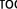
\includegraphics[width=0.4\textwidth]{label}
   \end{minipage}
\caption{ROLabel}
\label{fig:label}
\end{figure}

\begin{figure}[H]
      \begin{minipage}[t]{0.5\textwidth}
      \vspace{0pt}
     \begin{code}
     
	ROElement new 
		size: 100; 
		+ ROBorder.	\end{code}
   \end{minipage}
   \hfill
   \begin{minipage}[t]{0.4\textwidth}
      \vspace{0pt} \raggedright
       \centering
		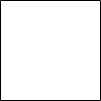
\includegraphics[width=0.25\textwidth]{border}
   \end{minipage}
\caption{ROBorder}
\label{fig:border}
\end{figure}  

\begin{figure}[H]
      \begin{minipage}[t]{0.5\textwidth}
      \vspace{0pt}
     \begin{code}
     
ROElement new 
	size: 200; 
	+ (ROBox new 
				color: Color green; 
				borderColor: Color red; 
				borderWidth: 4 ).	\end{code}
   \end{minipage}
   \hfill
   \begin{minipage}[t]{0.4\textwidth}
      \vspace{0pt} \raggedright
       \centering
		
\includegraphics[width=0.5\textwidth]{box}
   \end{minipage}
\caption{ROBox}
\label{fig:box}
\end{figure} 

\begin{figure}[H]
      \begin{minipage}[t]{0.5\textwidth}
      \vspace{0pt}
     \begin{code}
     
ROElement new 
	size: 100; 
	+ (ROCircle new 
				color: Color yellow; 
				borderColor: Color blue; 
				borderWidth: 2 ).	\end{code}
   \end{minipage}
   \hfill
   \begin{minipage}[t]{0.4\textwidth}
      \vspace{0pt} \raggedright
       \centering
		
\includegraphics[width=0.25\textwidth]{circle}     
   \end{minipage}
\caption{ROCircle}
\label{fig:circle}
\end{figure}



\paragraph{Composing Shapes.}
To create more complex looks we can compose shapes. To have an element shaped with more than one ROShape, we send the \ct{+} message several times with the desired shapes (\figref{composed}). This builds a chain of shapes associated to the element.
\sd{why do we need a cascade between shape? Is it key?}
\begin{figure}[H]
      \begin{minipage}[t]{0.5\textwidth}
      \vspace{0pt}
     \begin{code}
     
ROElement new 
	size: 180;  
	+ (ROLabel new text: 'composed shape');
	+ (ROBorder new color: Color red); 
	+ (ROCircle new color: Color yellow; 
					borderWidth: 0 ).	\end{code}
   \end{minipage}
   \hfill
   \begin{minipage}[t]{0.4\textwidth}
      \vspace{0pt} \raggedright
       \centering
		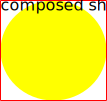
\includegraphics[width=0.4\textwidth]{composed}
   \end{minipage}
\caption{Composing shapes}
\label{fig:composed}
\end{figure} 

\subsubsection*{The Collection hierarchy example}
We now will add some shape to the classes in the \ct{Collection} hierarchy example. Each class representation will have a width according to the number of instance variables of the class and a height according to the number of its methods. Obtaining a polymetric representation of the class.

\begin{code}{}
view := ROView new.
classes := ROElement forCollection: Collection withAllSubclasses.
classes do: [:c | 
	c width: c model instVarNames size.
	c height: c model methods size.
	c + ROBorder. 
	c @ RODraggable ].
view addAll: classes.
ROHorizontalLineLayout new on: view elements.
view open.
\end{code}

\fig{H}{0.6}{hier2}{Adding some shape for each class}


%=====================
\section{Edges: linking elements} \seclabel{edges}

In Roassal it is possible to build links between elements to represent relationships between them. A link between elements is an instance of the class \ct{ROEdge}. An edge needs two elements: one to be the starting point and another to be the ending point. It is important to notice than an edge also needs to be shaped. The following code shows a very simple example of how to build an edge between two elements.
\sd{why there is no default for ROEdge shape and a EmptyShape?}
\sd{why do you need to say new in ROEdge?}

\begin{figure}[H]
 \begin{code}{}
view := ROView new.
startElement := (ROElement on: 1) size: 20; + ROBorder red.
endElement := (ROElement on: 2)  size: 20; + ROBorder red.
endElement translateBy: 50@50.

edge := ROEdge from: startElement to: endElement.
edge + ROLine new. "-> an edge needs to be shaped too"
view 
	add: startElement; 
	add: endElement; 
	add: edge. "-> and to be added to the visualization"
view inspect.
\end{code}   
\caption{Simple edge}
\label{fig:simpleEdge}
\end{figure} 

There are several ways to shape a ROEdge. Some examples are shown in \figref{line}, \figref{arrowEdge} and \figref{orthoEdge}.

\begin{figure}[H]
      \begin{minipage}[t]{0.5\textwidth}
      \vspace{0pt}
     \begin{code}{}
edge + ROLine new. \end{code}
   \end{minipage}
   \hfill
   \begin{minipage}[t]{0.4\textwidth}
      \vspace{0pt} \raggedright
       \centering
		\includegraphics[width=0.4\textwidth]{line}
   \end{minipage}
\caption{Simple edge}
\label{fig:line}
\end{figure} 

\begin{figure}[H]
      \begin{minipage}[t]{0.5\textwidth}
      \vspace{0pt}
     \begin{code}{}
edge + (ROLine new add: ROArrow new). \end{code}
   \end{minipage}
   \hfill
   \begin{minipage}[t]{0.4\textwidth}
      \vspace{0pt} \raggedright
       \centering
		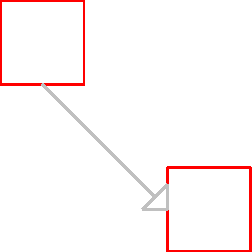
\includegraphics[width=0.4\textwidth]{arrowEdge}
   \end{minipage}
\caption{Arrowed edge}
\label{fig:arrowEdge}
\end{figure} 

\begin{figure}[H]
      \begin{minipage}[t]{0.5\textwidth}
      \vspace{0pt}
     \begin{code}{}
edge + (ROOrthoHorizontalLineShape new add: ROHorizontalArrow new)\end{code}
   \end{minipage}
   \hfill
   \begin{minipage}[t]{0.4\textwidth}
      \vspace{0pt} \raggedright
       \centering
		\includegraphics[width=0.4\textwidth]{orthoEdge}
   \end{minipage}
\caption{Orthogonal edge with horizontal oriented arrow}
\label{fig:orthoEdge}
\end{figure} 

\subsection*{The Collection hierarchy example}
Now we know how to make links between elements. With the following code we can create edges between each class to its superclass. To do so, we first need to create a collection of associations to build edges with them. Each association represents a starting point as the association key and an ending point as the association value. For this example each association goes from a \ct{ROElement} representing a class to a \ct{ROElement} that represents its superclass. After having the associations we create the instances of \ct{ROEdge} by using the \ct{linesFor:} selector.
\sd{the collect and select: sucks. why not simply using a do: and adding just what is needed.}

\begin{code}{}
view := ROView new.
classes := ROElement forCollection: Collection withAllSubclasses.
classes do: [:c | 
	c width: c model instVarNames size.
	c height: c model methods size.
	c + ROBorder. 
	c @ RODraggable ].
view addAll: classes.
associations := classes 
					collect: [:c | 	(c model superclass = Object)
										ifFalse: [ (view elementFromModel: c model superclass) -> c]]
					thenSelect: [:assoc | assoc isNil not ].
edges := ROEdge linesFor: associations.
view addAll: edges.
ROHorizontalLineLayout new on: view elements.
view open
\end{code}

\fig{H}{0.6}{hier3}{Adding links between each class and its superclass}

Now we have each class in the \ct{Collection} hierarchy with the shape we want and connected with each superclass. However we don't see a real hierarchy. This is because we need an appropriate layout to arrange all the elements of the view. Next section covers how to apply layouts to elements.


%=====================
\section{Layouts} \seclabel{layouts}
A layout defines how a collection of elements can be arranged automatically. Layouts inherits from the \ct{ROLayout} class. To apply a layout use the \ct{on:} message with a collection of \ct{ROElement}s as parameter, as shown in \figref{primerLayout}.


\begin{figure}[H]
\label{fig:primerLayout}
      \begin{minipage}[t]{0.5\textwidth}
      \vspace{0pt}
     \begin{code}{}
view := ROView new.
view 
	addAll: (ROElement spritesOn: (1 to: 4)).
ROGridLayout on: view elements.
view open.
  \end{code}
   \end{minipage}
   \hfill
   \begin{minipage}[t]{0.6\textwidth}
      \vspace{0pt} \raggedright
       \centering
		\includegraphics[width=0.3\textwidth]{ROGrid2} %layout1?
   \end{minipage}

\caption{ROGridLayout applied to a group of ROElements}
\end{figure} 

The message \ct{spriteOn:} creates a collection of ROElements, each with size equals to 50, shaped with a red border and draggable. Some of the layouts available in Roassal can be seen in \figref{roLayouts}. \sd{How do I find the other layout availbale}

\begin{figure} [H]
        \centering
		\subfigure[ROGridLayout]{
\includegraphics[width=0.15\textwidth]{ROGrid}} \hfill
		\subfigure[ROCircleLayout]{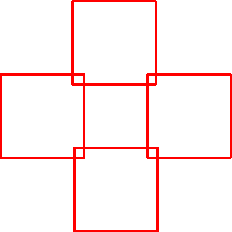
\includegraphics[width=0.15\textwidth]{ROCircle}}\hfill
		\subfigure[ROTreeLayout]{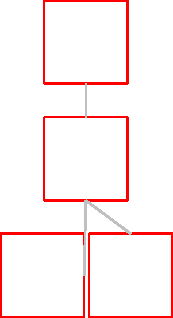
\includegraphics[width=0.11\textwidth]{ROTree}} \\ 
		\subfigure[ROMapTreeLayout]{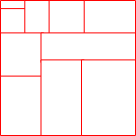
\includegraphics[width=0.2\textwidth]{ROMapTree}} \hfill
		\subfigure[ROVerticalLineLayout]{
\includegraphics[width=0.06\textwidth]{ROVertical}}\hfill
		\subfigure[ROHorizontalLineLayout]{
\includegraphics[width=0.25\textwidth]{ROHorizontal}}
        \caption{Some of the layouts available applied to a group of elements}\label{fig:roLayouts}
\end{figure}


\paragraph{Layouts in Nested Structures.}
When dealing with nested ROElements, layouts can \sd{are?} be relative to each element container.

\begin{figure}[H]
      \begin{minipage}[t]{0.61\textwidth}
      \vspace{0pt}
     \begin{code}{}
view := ROView new.
elements := (ROElement spritesOn: (1 to: 2)).
elements 
	do: [:el | el addAll: (ROElement spritesOn: (1 to: 3)). 
	           "arranging the children nodes"
			   ROGridLayout on: el elements.].			   
view addAll: elements.
ROHorizontalLineLayout on: view elements.
view open.
  \end{code}
   \end{minipage}
   \hfill
   \begin{minipage}[t]{0.6\textwidth}
      \vspace{0pt} \raggedright
       \centering
		
\includegraphics[width=0.6\textwidth]{nestedLayout}
   \end{minipage}
\label{fig:nestedLayout}
\caption{Nested elements with different layouts }
\end{figure} 

\subsection*{The Collection hierarchy example}
\sd{would be nice to have an example showing that you have different layout for certain nodes.}
As we need an hierarchy, the \ct{ROTreeLayout} will be useful to obtain the visualization we want.
\sd{why do we have @ RODraggable and + ROBorder}

\begin{figure}[H]
\begin{code}{}
view := ROView new.
classes := ROElement forCollection: Collection withAllSubclasses.

"Make each element reflect their model characteristics"
classes do: [:c | 
	c width: c model instVarNames size.
	c height: c model methods size.
	c + ROBorder. 
	c @ RODraggable ].
view addAll: classes.

"Add edges between each class and its superclass (or its subclasseS)"
associations := classes collect: [:c | 
	(c model superclass = Object)
		ifFalse: [ (view elementFromModel: c model superclass) -> c]
	 ] thenSelect: [:assoc | assoc isNil not ].
edges := ROEdge linesFor: associations.
view addAll: edges.

"Arrange all the elements as a hierarchy"
ROTreeLayout new on: view elements.
view open
\end{code}
\end{figure}

We did it! :) \vp{<-ok, maybe remove this} The resulting visualization can be seen in \figref{collectionHierarchy}.

\fig{H}{0.4}{collectionHierarchy}{Collection class hierarchy with width reflecting instance variable number and height number of methods.}

%=====================

\section{Events and Callbacks}

Roassal allows any visible component in a visualization, including itself, to react to events. There are two kinds of events defined in Roassal. In the first kind are those responding to external events, like mouse clicks, mouse move or key press. The second kind of events includes those triggered by internal manipulation of the ROView or its components, like when a view needs to be refreshed. All events inherits from the \ct{ROEvent} class.

To see how events work, we define a visualization to react to mouse clicks, translating an element to where the click was made. 
There are several event classes to deal with mouse events: \ct{ROMouseClick}, \ct{ROMouseMove}, \ct{ROMouseEnter} and \ct{ROMouseLeave}, among others; and to deal with key pressing, the \ct{ROKeyDown} class.
We will make the visualization to react to the left click of the mouse using the \ct{ROLeftMouseClick} event. The reaction will create an animation to translate the element to the event position.


\begin{code}{}
view := ROView new.
el := ROElement sprite.
view add: el.
view 
	on: ROMouseLeftClick 
	do: [ :event | 
	        ROLinearMove new	for: el to: event position].
view open. 
\end{code}

We use the \ct{on:do:} message to set a Roassal object to react to an event. The first parameter must be the class of the expected event and the second one a block which defines the action to be executed when the event is received.

\ct{ROLinearMove} is one of the Roassal interactions. As its name suggest, it creates an animation for an element to be translated in a linear move. More about interactions are explained in next section.

%
%\alex{How to define callbacks}
%\alex{What are the different events we can handle}


%=====================
\section{The interaction hierarchy} \seclabel{interactions}

A ROElement can respond to events by setting callbacks or interactions. We already presented how to set callbacks, so here we will show the interactions. 

The root class of all Roassal interactions is \ct{ROInteraction}. An interaction is set to an element by sending the \ct{@} message with an instance of \ct{ROInteraction} as parameter. There are diverse interactions that can be set to a Roassal element \sd{such what?}.
 \ct{RODraggable} allows an element to be dragged by the mouse and \ct{ROGrowable} makes an element to increase its size when clicked. Try the following code. Click the element to make it bigger and drag it to move it on the view.

\begin{code}{}
|view element|
view := ROView new.
element := ROElement new size: 10.
element 
	+ ROBox;
	@ RODraggable; 
	@ ROGrowable.
view add: element.
view open.
\end{code}


Some interactions are more complex like popups elements, displayed when the mouse is over an element. 

%There are interactions that makes elements to react to events, such as \ct{RODraggable}, that allows an element to be dragged by the mouse, or \ct{ROGrowable}, that makes an element to increase its size when clicked. Some of this interactions are more complex like popups elements, accesible by the subclasses of \ct{ROAbstractPopup}, which are displayed when the mouse is over an element. 

\subsection{Animations} Animations are also interactions in Roassal. Some animations allows elements to be translated, like \ct{ROLinearMove}. \ct{ROZoomInMove} and \ct{ROZoomOutMove} zoom in or out, respectively. All animations are subclasses of \ct{ROAnimation}.

From the availables interactions in Roassal, two examples are presented: one for \ct{ROAbstractPopup} and one for \ct{ROAnimation}.

\subsubsection*{ROAbstractPopup}

\ct{ROAbstractPopup} allows elements to react to mouse over events by displaying a popup. There are two kind of popups, (i) \ct{ROPopup}, which by default displays a box with the string representation of the element value \sd{is printString used?}; and (ii) \ct{ROPopupView} that displays a custom view.

To add a popup to an element just send the \ct{@} message with the \ct{ROPopup} class as argument. It is also possible to setup a custom text using the \ct{text:} message with a custom string.
\sd{I do not understand ROElement spriteOn: 'Roassal'.}

\begin{figure}[H]
      \begin{minipage}[t]{1\textwidth}
      \vspace{0pt}
     \begin{code}{}
view := ROView new.
el := ROElement spriteOn: 'Roassal'.
el @ ROPopup. "Or with custom text -> (ROPopup text: 'this is custom text')"
view add: el.
view open.
  \end{code}
   \end{minipage}
   \hfill
   \begin{minipage}[t]{1\textwidth}
	 \vspace{0pt} \raggedright
       \centering
		\includegraphics[width=0.7\textwidth]{popup}
   \end{minipage}
\label{fig:popup}
\caption{ROPopup}
\end{figure} 

\ct{ROPopupView} is slightly more complex as it needs the definition of the view to popup. This interaction can be created by sending the \ct{view:} message to the \ct{ROPopupView} class with the view to be displayed. The parameter can also be a block with one value to be evaluated with the element where the interaction belongs to. \sd{unclears}

The following example creates a view with five elements. Each one reacts when the mouse is over by displaying a popup. The popup is defined as a block which creates a view with the same amount of nodes as the element model where the mouse is. For example, and as \figref{popupView} shows, when passing the mouse over the node ``3'', a popup with \textit{three} gray boxes appears.
\sd{cool example!}
\begin{figure}[H]
      \begin{minipage}[t]{1\textwidth}
      \vspace{0pt}
     \begin{code}{}
view := ROView new.
elements := ROElement spritesOn: (1 to: 5).
"create the view to popup"
viewToPopup := [ :el | |v| 
	              	              v := ROView new.
	              	              "Add as much elements as the value represented"
	              	              v addAll: (ROElement forCollection: (1 to: el model)).
	              	              v elementsDo: [ :e | e size: 20; + ROBox ].
	              	              ROGridLayout on: v elements.
	              	              v ].
elements do: [ :e | e + ROLabel;  @ (ROPopupView view: viewToPopup)].
view addAll: elements.
ROHorizontalLineLayout on: view elements.
view open.
\end{code}
\end{minipage}\hfill\begin{minipage}[t]{1\textwidth}
	 \vspace{0pt} \raggedright
       \centering
		\includegraphics[width=0.7\textwidth]{popupView2}
   \end{minipage}
\label{fig:popupView}
\caption{\ct{ROPopupView} \sd{better title please}}
\end{figure} 


%first example
%view := ROView new.
%el := ROElement spriteOn: 'Roassal'.
%
%"create the view to popup"
%viewToPopup := ROView new.
%viewToPopup 
%	addAll: (ROElement forCollection: (1 to: 4 )).
%viewToPopup 
%	elementsDo: [:e | e size: 20. e + ROBox  ].
%ROGridLayout 
%	on: viewToPopup elements.
%	
%el := ROElement spriteOn: 'Roassal'.
%el @ (ROPopupView view: viewToPopup).
%view add: el.
%view open.


%
%\vp{not sure if present this one}
%\subsubsection*{ROMenuActivable}
%
%\begin{figure}[H]
%      \begin{minipage}[t]{1\textwidth}
%      \vspace{0pt}
%     \begin{code}{}
%view := ROView new.
%el := ROElement sprite.
%el @ (ROMenuActivable new item: 'inspect' action: #inspect).
%view add: el.
%view open.
%  \end{code}
%   \end{minipage}
%   \hfill
%   \begin{minipage}[t]{1\textwidth}
%	 \vspace{0pt} \raggedright
%       \centering
%		\includegraphics[width=0.7\textwidth]{menuActivable}
%   \end{minipage}
%\label{fig:menuActivable}
%\caption{ROMenuActivable applied to a ROElement}
%\end{figure} 

\subsubsection*{\ct{ROAnimation}}
Any animation is an instance of a subclass of the \ct{ROAnimation} class. Some examples are \ct{ROLinearMove}, \ct{ROZoomInMove} and \ct{ROZoomOutMove}.

Each animation has a number of cycles to complete, executing each one by sending the \ct{doStep} message.
A \ct{ROAnimation} also allows one to set a block to be executed after the animation is finished, using the \ct{after:} message. It is important to notice that any action to be done after the animation is finished must be set before the animation is triggered, otherwise it will not be executed. \sd{do you have a before: message.}

\figref{mouseClick} presents \ct{ROLinearMove}. The following code allows an element to be animated in a sin curve, using the \ct{ROFunctionMove}.

\begin{figure}[H]
\begin{code}{}
view := ROView new.

element := ROElement new.
element size: 10.
element + (ROCircle color: Color green).

view add: element.
element translateBy: 30@20.

ROFuncionMove new
	nbCycles: 360;
	blockY: [ :x | (x * 3.1415 / 180) sin * 80 + 50 ];
	on: element.
view open.
\end{code}
\end{figure}

%\alex{Present the hierarchy of the interaction}

%\alex{Give some examples with buttons and animations}


%=====================
\section{Understanding Camera} \seclabel{camera}

A view's camera represents the point of view from \sd{which} it is actually viewed. It has a position, where it is located on the visualization; an extent, which is what we are seeing; a real extent which represents the far extent and the window size of the visualization. A camera's directions is always perpendicular to the view. \sd{it would be good to have a diagram to show.}
\sd{what about a height method}

The extent of the view's camera affects the way a view is drawn in a canvas. When rendering a view, each point, rectangle or other shape that needs to be drawn will be plotted according to the camera extent. This is done by transforming each absolute position or size in \emph{virtual} points or rectangles relative to the camera's vision.

When \ct{translateBy:} or \ct{translateTo:} are called by a view, what actually happens is that its camera moves, no the visualization itself. And changing the altitude simulates the zooming facility of Roassal \sd{how can we change the altitude?}. By moving the camera down (\ie the view is zoomed in), it changes what will be shown: it defines a smaller rectangle that must be adapted to the real extent, and because of this making everything bigger.% the position and extent of the camera changes, defining smaller bounds and seeing everything bigger. 

This is used by the \ct{ROZoomMove}, which is used by \ct{ROZoomInMove} and \ct{ROZoomOutMove}. This is also used by the \ct{ROMiniMap} interaction.

The \ct{ROMiniMap} allows one to have a complete vision of a visualization for better navigation. It is composed of a smaller version of the visualization and a ``lupa'', which represents the current visible part of the view's window. To add this interaction, just send the \ct{@ROMiniMap} message to a view and press ``m'' to open it (\figref{miniMap}). \sd{how the communication between the MiniMap and the other view is done?}

\fig{H}{0.9}{miniMap}{\ct{ROMiniMap} applied to the Collection Hierarchy example}

The smaller version of the view is displayed by a \ct{ROMiniMapDisplayer}, subclass of \ct{ROViewDisplayer}. 
As their name suggest it, they are shapes that display a view on a ROElement. The difference between both is that \ct{ROMiniMapDisplayer} uses its own camera, which has a different extent to the view's camera. This allows \sd{one} to see the same view with different size. 

The lupa  size represents the visible part of the window and its position is related to the view's camera position. When the view is translated to a point, the lupa follows it by changing its position: the point representing the camera position is translated to a point on the \ct{ROMiniMapDisplayer} camera extent. And when the view is zoomed in or zoomed out the extent of the camera is changed, increasing o decreasing the lupa's size.

%\alex{MiniMap}
%\alex{Semantic zooming: Making objects appear when the camera goes down}

%=====================
\section{The Mondrian DSL}
\sd{Mondrian is an older visualization framework developed by D. Girba and M Meer and maintained by A. Bergel. It influenced the design of Roassal. It supports visualization scripting based on a dedicated DSL: the DSL is based on a stack model where elements on the top can be parametrized. Roassal is designed to be a flexible framework and it is not tight to a DSL. Now Roassal can be extended to support Mondrian-like DSL scripting. This is what we present in this Section.}


A \ct{ROMondrianViewBuilder} models the Mondrian DSL\footnote{\url{http://www.moosetechnology.org/tools/mondrian}}. It is mostly compatible with the original Mondrian language.% (cf., Mondrian paper and website).

%ROMondrianBuilder acts as a translation between the Mondrian DSL and the Roassal model.
A \ct{ROMondrianViewBuilder} internally contains an instance of a \ct{ROView}, called raw view. Its accessor is \ct{raw}. All scripting  using the \ct{ROMondrianViewBuilder} result in creating \ct{ROElement}s with the shapes and interactions set by the script, and added to the raw view. To start a visualization with the builder, you can use the following code:

\begin{code}{}
view := ROMondrianViewBuilder new.
view open.
\end{code}

A Mondrian builder can also be initialized with an instance of a ROView. However it is important to understand that this is not required, as the builder by default will create its own raw view.
When working with the builder, is it possible to use the Mondrian DSL, sending messages to an instance of the \ct{ROMondrianViewBuilder}, or directly with the raw view. %However the main benefit of the builder it to use the Mondrian scripting.

\begin{code}{}
rawView := ROView new.
view := ROMondrianViewBuilder view: rawView.
view open.
\end{code}

A small summary of the Mondrian DSL is offered here. To more detailed information, please refer to the dedicated Moose book chapter~\footnote{\url{http://themoosebook.org/book/internals/mondrian}}.

To add a node to the visualization, which be internally translated as a ROElement later on, use the selector \ct{node:} with the object you want to represent on the instance of the builder.

\begin{figure}[H]
      \begin{minipage}[t]{1\textwidth}
      \vspace{0pt}
\begin{code}{}
view := ROMondrianViewBuilder new.
view node: 1.
view open.
\end{code}
   \end{minipage}
   \hfill
   \begin{minipage}[t]{1\textwidth}
	 \vspace{0pt} \raggedright
       \centering
		\includegraphics[width=0.7\textwidth]{mondrian1}
   \end{minipage}
\label{fig:mondrian1}
\end{figure} 




To define shapes, use the \ct{shape} message followed by the desired shape with its characteristics, before the node or nodes definition. This will locally define the shape for the nodes.

\begin{figure}[H]
      \begin{minipage}[t]{1\textwidth}
      \vspace{0pt}
\begin{code}{}
view := ROMondrianViewBuilder new.
view shape rectangle 
	size: 10;
	color: Color red.
view node: 1.
view open.
\end{code}
   \end{minipage}
   \hfill
   \begin{minipage}[t]{1\textwidth}
	 \vspace{0pt} \raggedright
       \centering
		\includegraphics[width=0.7\textwidth]{mondrian2}
   \end{minipage}
\label{fig:mondrian2}
\end{figure} 


By using the \ct{nodes:} message with a collection of objects you can create several nodes.

\begin{figure}[H]
      \begin{minipage}[t]{1\textwidth}
      \vspace{0pt}
\begin{code}{}
view := ROMondrianViewBuilder new.
view shape rectangle 
	size: 10;
	color: Color red.
view nodes: (1 to: 5).
view open.
\end{code}
   \end{minipage}
   \hfill
   \begin{minipage}[t]{1\textwidth}
	 \vspace{0pt} \raggedright
       \centering
		\includegraphics[width=0.7\textwidth]{mondrian3}
   \end{minipage}
\label{fig:mondrian3}
\end{figure} 

If the node or nodes have nested nodes, use the \ct{node:forIt:} or \ct{nodes:forEach:} message to add them. The second parameter is a block which will add the nested nodes, as the following code shows:

\begin{figure}[H]
      \begin{minipage}[t]{1\textwidth}
      \vspace{0pt}
\begin{code}{}
view := ROMondrianViewBuilder new.
view shape rectangle 
	size: 10;
	color: Color red.
view 
	nodes: (1 to: 5) 	
	forEach:[:each |
		view shape rectangle 
			size: 5;
			color: Color yellow.
		view nodes: (1 to: 2).
	].
view open.
\end{code}
   \end{minipage}
   \hfill
   \begin{minipage}[t]{1\textwidth}
	 \vspace{0pt} \raggedright
       \centering
		\includegraphics[width=0.7\textwidth]{mondrian4}
   \end{minipage}
\label{fig:mondrian4}
\end{figure} 



%The shapes must be defined before the nodes definition.
%To define shapes, use the \#shape selector followed by the desired shape with its characteristics, before the node or nodes definition. This will locally define the shape for the nodes.

%\begin{code}{}
%view := ROMondrianViewBuilder new.
%view shape rectangle size: 20.
%view node: 1 forIt:[
%	view shape rectangle size: 20; color: Color red.
%	view nodes: (1 to: 3)
%].
%view open.
%\end{code}

It is possible to create edges by using the \ct{edgesFromAssociations:} message with a collection of associations between the model of the nodes.

\begin{figure}[H]
      \begin{minipage}[t]{1\textwidth}
      \vspace{0pt}
\begin{code}{}
view := ROMondrianViewBuilder new.
view shape rectangle 
	color: Color red.
view nodes: (1 to: 4).
view 
	edgesFromAssociations: (Array with: 1-> 2 with: 2 -> 3 with: 2 -> 4).
view open.
\end{code}
   \end{minipage}
   \hfill
   \begin{minipage}[t]{1\textwidth}
	 \vspace{0pt} \raggedright
       \centering
		\includegraphics[width=0.7\textwidth]{mondrian5}
   \end{minipage}
\label{fig:mondrian5}
\end{figure} 



Similar to the \ct{Collection} hierarchy example we need an appropriate layout. By default the builder applies a horizontal line layout and we need a tree layout. We use the \ct{treeLayout} to apply it.

\begin{figure}[H]
      \begin{minipage}[t]{1\textwidth}
      \vspace{0pt}
\begin{code}{}
view := ROMondrianViewBuilder new.
view shape rectangle 
	size: 10;
	color: Color red.
view nodes: (1 to: 4).
view edgesFromAssociations: (Array with: 1-> 2 with: 2 -> 3 with: 2 -> 4).
view treeLayout.
view open.
\end{code}
   \end{minipage}
   \hfill
   \begin{minipage}[t]{1\textwidth}
	 \vspace{0pt} \raggedright
       \centering
		\includegraphics[width=0.7\textwidth]{mondrian6}
   \end{minipage}
\label{fig:mondrian6}
\end{figure} 




\subsection*{The Collection Hierarchy example}

The Mondrian DSL allows a simpler scripting to the Collection hierarchy visualization than the one constructed through the chapter. By setting how each element and edge must be created, it is not necessary for us to create them by hand.
The following code can be replaced for the earlier version:

\begin{code}{}
view := ROMondrianViewBuilder new.
view shape rectangle
	width: [ :cls | cls instVarNames size ]; 
	height: [ :cls | cls methods size ].
view nodes: Collection withAllSubclasses.
view edgesFrom: #superclass.
view treeLayout.
view open.
\end{code}

%=====================
\section{Roassal Easel}


Pharo's World menu offers an item for launching the Easel. The easel is composed by two windows, the one on the left-hand side contains the visualization and the one in the right hand a workspace containing the script to be executed. By accepting (Cmd-S, Alt-S) in the editor, the changes will be displayed in the visualization window.

The easel offers lots of examples to see visualizations and learn how to make them, including a tutorial separated by steps. Examples are separated in two categories: \textbf{ROMondrianViewBuilder} and \textbf{ROExample}.

The first category includes examples done with the builder, using Mondrian DSL to make each script. The second one shows examples of how do directly interact with the \ct{ROView} class, making possible to reproduce them without the builder.

It also includes how to add buttons to zoom in and zoom out the visualization, export it to different formats and save it, among other actions. This buttons are not included by default in the Mondrian builder or the ROView, so the easel teach how to do it.
%=====================
\section{Beyond Pharo}

Roassal have been designed to be easily ported to other Smalltalk dialects. Currently it has been ported to VisualWorks, Amber and VA Smalltalk.

As \figref{structure} shows, Roassal consists in three main components:

\begin{itemize}
\item  The Roassal Core, a set of packages that contains all the main classes definition, like ROView, ROElement, ROShape and ROCamera. It also contains all the tests.
\item The Mondrian DSL, composed by the Roassal-Builder and Roassal-Builder-Tests packages.
\item The platform dependent packages, that is dedicated to each Smalltalk dialect Roassal is ported to.
\end{itemize} 

In top of this components, you application will be build.

In the platform dependent packages several classes must be implemented. The main ones are a native canvas class, where a view can be rendered, and a widget factory class, which can return an object to contain the canvas and receive and delegate all the external events.
The first must be subclass of ROAbstractCanvas and the second must be subclass of RONativeWidgetFactory.

The \ct{ROPlatform} class defines how the bridge between the core and the dependent packages must be implemented. This class defines instance variables, like \ct{canvasClass} and \ct{widgetFactory}, which store the correspondent class to use according to their name. Each platform dependent package must implement its own platform class, make it subclass of ROPlatform and reference all the implemented platform dependent classes.
Internally, every time one of this classes is needed, the core relies in the current instance of a ROPlatform to return the needed class.

\fig{H}{0.3}{structure}{Roassal structure}

%\alex{Describe the platform architecture}

%=====================

\section{Conclusion}

Roassal enables any graph of objects to be visualized. This chapter has reviewed the main features of Roassal:

\begin{itemize}
\item Create graphical elements
\item Shape them and make them look as desired
\item Make them react to events
\item Apply layouts to a view elements for them to be arranged automatically 
\item The builder to create a view using Mondrian DSL
\end{itemize}

\paragraph{Acknowledgment}
We are very grateful to Nicolas Rosselot Urrejola for his review of an early draft of the chapter.

%Mondrian is a perpetual evolving application. This chapter intents to cover the features frequently used. If there is a topic you wish to see discussed here, send an email to alexandre@bergel.eu.
%
%We hope you haved enjoyed it!
%
%=====================


%=============================================================
\ifx\wholebook\relax\else
   \bibliographystyle{jurabib}
   \nobibliography{scg}
   \end{document}
\fi
%=============================================================


%Dead text:

Node color \ja{nothing about edge color ? I think we can say that it is possible too} is an important information support, as the width and the height of a node. Color should be easy to pick to represent particular condition.

The keyword if:fillColor: enables one to assign a color for a particular condition. Consider we want to extend the previous example by coloring abstract classes in red.

\begin{code}{}
view shape rectangle
  width: [ :each | each instVarNames size * 3 ];
  height: [ :each | each methods size ];
  if: #isAbstractClass fillColor: Color red.
view nodes: Collection withAllSubclasses.

view edges: Collection withAllSubclasses from: #yourself toAll: #subclasses.

view treeLayout.
\end{code}


The message \ct{if:fillColor:} may be sent to a shape to conditionally set a color. \ja{what is the link with the source code below ?}

\begin{code}{}
view shape rectangle
  width: [ :each | each instVarNames size * 3];
  height: [ :each | each methods size ];
  if: #isAbstractClass fillColor: Color red.
view nodes: Collection withAllSubclasses.

view edgesFrom: #superclass.

view treeLayout.
\end{code}

All red nodes represent abstract class. Waving the moose above a node make a text tooltip appear revealing its name. 

\ja{it should not be here, we are in section 'adding colors'}
Extended possibilities exist to define interaction. We will review them in a future section. For now, if you are interested in opening a system browser directly from a node, you define this interaction: \ja{can you display only the line concerned ? it is difficult to read each time the same code with only one line changed}

\begin{code}{}
view interaction action: #browse.
view shape rectangle
  width: [ :each | each instVarNames size * 3];
  height: [ :each | each methods size ];
  if: #isAbstractClass fillColor: Color red.
view nodes: Collection withAllSubclasses.

view edgesFrom: #superclass.

view treeLayout.
\end{code}

You can easily \ja{I think there are too much 'easy' or 'easily' in the chapter} spot some red node that do not have subclasses. This indicates a design flow since an abstract must to have subclasses. It makes no sense for a class that is not supposed to be instantiated (since it is abstract) to not have a subclass.

The very same analyzes can be realized on your own classes.

\ja{is this code useful ? it seems to be the same as above}

\begin{code}{}
view interaction action: #browse.
view shape rectangle
  width: [ :each | each instVarNames size * 3];
  height: [ :each | each methods size ];
  if: #isAbstractClass fillColor: Color red.
view nodes: (PackageInfo named: 'Mondrian') classes.

view edgesFrom: #superclass.

view treeLayout.
\end{code}

A shape may contains more than one condition. Let's distinguish abstract classes from classes that define abstract methods.

\begin{code}{}
view shape rectangle
  width: [ :each | each instVarNames size * 3];
  height: [ :each | each methods size ];
  if: #isAbstractClass fillColor: Color lightRed;
  if: [:cls | cls methods anySatisfy: #isAbstract ] fillColor: Color red.

view nodes: Collection withAllSubclasses.

view edgesFrom: #superclass.

view treeLayout.
\end{code}

All red nodes are still abstract classes. Light red indicates classes that do not define abstract methods; strong red indicates classes that define at least one abstract method.

%-----------------------------------------------------------------

%%% Local Variables:
%%% coding: utf-8
%%% mode: latex
%%% TeX-master: t
%%% TeX-PDF-mode: t
%%% ispell-local-dictionary: "english"
%%% End:

% FINISHED



%=================================================================
\ifx\wholebook\relax\else
% --------------------------------------------
% Lulu:
	\documentclass[a4paper,10pt,twoside]{book}
	\usepackage[
		papersize={6.13in,9.21in},
		hmargin={.75in,.75in},
		vmargin={.75in,1in},
		ignoreheadfoot
	]{geometry}
	\input{../common.tex}
	\setboolean{lulu}{true}
% --------------------------------------------
% A4:
%	\documentclass[a4paper,11pt,twoside]{book}
%	\input{../common.tex}
%	\usepackage{a4wide}
% --------------------------------------------
    \graphicspath{{figures/} {../figures/}}
	\begin{document}
\fi
%=================================================================
%\renewcommand{\nnbb}[2]{} % Disable editorial comments
\sloppy
%=================================================================
\chapter{Scripting Visualizations with Mondrian}
\chalabel{mondrian}

\indent

Attaching a meaning to a large amount of data is challenging without adequate tools. Textual outputs are known to be limited in their expression and interactions. 

Mondrian is a Domain Specific Language to script visualizations. Its latest implementation runs on top of Roassal (see Chapter~\ref{cha:roassal}).  
It is made to visualize and interact with any arbitrary data, defined in terms of objects and their relationships. Mondrian is commonly employed in software assessment activities. Mondrian excels at visualizing software source code. 
This chapter introduces Mondrian's principles and describes its expressive commands to quickly make up your data. For more detailed information, please refer to the dedicated Moose book chapter~\footnote{\url{http://themoosebook.org/book/internals/mondrian}}.
After reading it, you will be able to create interactive and visual representations.

%=====================

\section{Installation and first visualization}

Mondrian is based on Roassal. Check the Roassal chapter for installation procedures. If you are using a Moose distribution of Pharo \footnote{\url{http://www.moosetechnology.org/}}, then you already have Roassal. 

\subsection{A First Visualization}
You can get a first visualization by entering and executing the following code in a workspace. By executing the following in a workspace, you should see the Collection class hierarchy.

\begin{code}{}
| view |
view := ROMondrianViewBuilder new.
view shape rectangle 
	width:  [ :cls | cls numberOfVariables * 5 ];  
	height: #numberOfMethods;
	linearFillColor: #numberOfLinesOfCode within:  Collection withAllSubclasses.
view interaction action: #browse.
view nodes: ROShape withAllSubclasses.
view edgesFrom: #superclass.
view treeLayout.
view open
\end{code}

The visualization should be read as follows:

\begin{itemize}
\item each class is graphically represented as a box
\item inheritance is indicated with edges between boxes. A superclass is above its subclasses
\item the \emph{width} of each class indicates the amount of instance variable 
\item the \emph{height} of a class indicates the amount of methods defined in the class. The taller the class is, the more methods it defines.
\item the class \emph{shading} indicates the amount of lines of code the class contains. The class colored in black contains the most lines of code. The white class contains the smallest quantity of lines of code.
\end{itemize}

We will detail and review all the mechanisms involved in the visualization later on.


\section{Starting with Mondrian}

A \ct{ROMondrianViewBuilder} models the Mondrian domain-specific language (DSL).
A \ct{ROMondrianViewBuilder} internally contains an instance of a \lct{ROView}, called raw view. Its accessor is \ct{raw}. All scripting  using the \ct{ROMondrianViewBuilder} result in creating \ct{ROElement}s with the shapes and interactions set by the script, and added to the raw view. To start a visualization with the builder, you can use the following code:

\begin{code}{}
view := ROMondrianViewBuilder new.
view open.
\end{code}

A Mondrian builder can also be initialized with an instance of a ROView. It, however, is important to understand that this is not required, as the builder by default will create its own raw view.
When working with the builder, it is possible to use the Mondrian DSL, sending messages to an instance of the \ct{ROMondrianViewBuilder}, or directly with the raw view. 

\begin{code}{}
rawView := ROView new.
view := ROMondrianViewBuilder view: rawView.
view open.
\end{code}

To add a node to the visualization, which is internally translated as a ROElement later on, use the selector \ct{node:} with the object you want to represent. By default, a small square is drawn for each element.

\begin{figure}[H]
      \begin{minipage}[t]{1\textwidth}
      \vspace{0pt}
\begin{code}{}
view := ROMondrianViewBuilder new.
view node: 1.
view open.
\end{code}
   \end{minipage}
   \hfill
   \begin{minipage}[t]{1\textwidth}
	 \vspace{0pt} \raggedright
       \centering
		\includegraphics[width=0.7\textwidth]{mondrian1}
   \end{minipage}
\label{fig:mondrian1}
\end{figure} 




To define shapes, use the \ct{shape} message followed by the desired shape with its characteristics, before the node or nodes definition. This will locally define the shape for the nodes.

\begin{figure}[H]
      \begin{minipage}[t]{1\textwidth}
      \vspace{0pt}
\begin{code}{}
view := ROMondrianViewBuilder new.
view shape rectangle 
	size: 10;
	color: Color red.
view node: 1.
view open.
\end{code}
   \end{minipage}
   \hfill
   \begin{minipage}[t]{1\textwidth}
	 \vspace{0pt} \raggedright
       \centering
		\includegraphics[width=0.7\textwidth]{mondrian2}
   \end{minipage}
\label{fig:mondrian2}
\end{figure} 


By using the \ct{nodes:} message with a collection of objects you can create several nodes.

\begin{figure}[H]
      \begin{minipage}[t]{1\textwidth}
      \vspace{0pt}
\begin{code}{}
view := ROMondrianViewBuilder new.
view shape rectangle 
	size: 10;
	color: Color red.
view nodes: (1 to: 5).
view open.
\end{code}
   \end{minipage}
   \hfill
   \begin{minipage}[t]{1\textwidth}
	 \vspace{0pt} \raggedright
       \centering
		\includegraphics[width=0.7\textwidth]{mondrian3}
   \end{minipage}
\label{fig:mondrian3}
\end{figure} 

If the node or nodes have nested nodes, use the \ct{node:forIt:} or \ct{nodes:forEach:} message to add them. The second parameter is a block which will add the nested nodes, as the following code shows:

\begin{figure}[H]
      \begin{minipage}[t]{1\textwidth}
      \vspace{0pt}
\begin{code}{}
view := ROMondrianViewBuilder new.
view shape rectangle 
	size: 10;
	color: Color red.
view 
	nodes: (1 to: 5) 	
	forEach: [ :each |
		view shape rectangle 
			size: 5;
			color: Color yellow.
		view nodes: (1 to: 2) ].
view open.
\end{code}
   \end{minipage}
   \hfill
   \begin{minipage}[t]{1\textwidth}
	 \vspace{0pt} \raggedright
       \centering
		\includegraphics[width=0.7\textwidth]{mondrian4}
   \end{minipage}
\label{fig:mondrian4}
\end{figure} 



%The shapes must be defined before the nodes definition.
%To define shapes, use the \#shape selector followed by the desired shape with its characteristics, before the node or nodes definition. This will locally define the shape for the nodes.

%\begin{code}{}
%view := ROMondrianViewBuilder new.
%view shape rectangle size: 20.
%view node: 1 forIt:[
%	view shape rectangle size: 20; color: Color red.
%	view nodes: (1 to: 3)
%].
%view open.
%\end{code}

It is possible to create edges by using the \ct{edgesFromAssociations:} message with a collection of associations between the model of the nodes.

\begin{figure}[H]
      \begin{minipage}[t]{1\textwidth}
      \vspace{0pt}
\begin{code}{}
view := ROMondrianViewBuilder new.
view shape rectangle 
	color: Color red.
view nodes: (1 to: 4).
view edgesFromAssociations: (Array with: 1-> 2 with: 2 -> 3 with: 2 -> 4).
view open.
\end{code}
   \end{minipage}
   \hfill
   \begin{minipage}[t]{1\textwidth}
	 \vspace{0pt} \raggedright
       \centering
		\includegraphics[width=0.7\textwidth]{mondrian5}
   \end{minipage}
\label{fig:mondrian5}
\end{figure} 



Similar to the \ct{Collection} hierarchy example, given at the beginning of the chapter, we need an appropriate layout. By default the builder applies a horizontal line layout and we need a tree layout. We use the \ct{treeLayout} to apply it.

\begin{figure}[H]
      \begin{minipage}[t]{1\textwidth}
      \vspace{0pt}
\begin{code}{}
view := ROMondrianViewBuilder new.
view shape rectangle 
	size: 10;
	color: Color red.
view nodes: (1 to: 4).
view edgesFromAssociations: (Array with: 1-> 2 with: 2 -> 3 with: 2 -> 4).
view treeLayout.
view open.
\end{code}
   \end{minipage}
   \hfill
   \begin{minipage}[t]{1\textwidth}
	 \vspace{0pt} \raggedright
       \centering
		\includegraphics[width=0.7\textwidth]{mondrian6}
   \end{minipage}
\label{fig:mondrian6}
\end{figure} 




\subsection*{The Collection Hierarchy example}

The Mondrian DSL allows a simpler scripting to the Collection hierarchy visualization than the one constructed through the chapter. By setting how each element and edge must be created, it is not necessary for us to create them by hand.

\begin{code}{}
view := ROMondrianViewBuilder new.
view shape rectangle
	width: [ :cls | cls instVarNames size ]; 
	height: [ :cls | cls methods size ].
view nodes: Collection withAllSubclasses.
view edgesFrom: #superclass.
view treeLayout.
view open.
\end{code}


There are essentially two ways to work with Mondrian, either using the easel or a view renderer. The easel is a tool in which users may interactively and incrementally build a visualization by means of a script.  The easel is particularly useful when prototyping.
\ct{MOViewRenderer} enables a visualization to be programmatically built, in a non-interactive fashion. You probably want to use this class when embedding your visualization in your application.

We will first use Mondrian in its easiest way, by using the easel. To open an easel, you can either use the World menu (it should contain the entry ``Mondrian Easel'') or execute the expression:

\begin{code}{}
ROEaselMorphic open.
\end{code}


In the easel you have just opened, you can see two panels: the one on top is the visualization panel, the second one is the script panel. In the script panel, enter the following code and press the \emph{generate} button:

\begin{code}{}
view nodes: (1 to: 20).
\end{code}
\begin{center}\includegraphics[scale=0.34]{picture1}\end{center}

You should see in the top pane 20 small boxes lined up in the top left corner. You have just rendered the numerical set between 1 and 20. Each box represents a number. The amount of interaction you can do is quite limited for now. You can only drag and drop a number and get a tooltip that indicates its value. We will soon see how to define interactions. For now, let us explore the basic drawing capabilities of Mondrian.

We can add edges between nodes that we already drawn. Add a second line:

\begin{code}{}
view nodes: (1 to: 20).
view edgesFrom: [ :v | v * 2 ].
\end{code}
\begin{center}\includegraphics[scale=0.4]{picture2}\end{center}

Each number is linked with its double. Not all the doubles are visible. For example, the double of 20 is 40, which is not part of the visualization. In that case, no edge is drawn. 

The message \ct{edgesFrom:} defines one edge per node, when possible. For each node that has been added in the visualization, an edge is defined between this node and a node lookup from the provided block.

Mondrian contains a number of layouts to order nodes. Here, we use the circle layout:

\begin{code}{}
view nodes: (1 to: 20).
view edgesFrom: [ :v | v * 2 ].
view circleLayout.
\end{code}

The visualization you obtain is:

\begin{center}\includegraphics[scale=0.4]{picture3}\end{center}

In the subsequent section we will visualize software code to illustrate the power of Mondrian. Visualizing source code is often employed to discover patterns, useful when assessing code quality.

%=====================

\section{Visualizing the Collection framework}

We will now visualize Pharo classes. For the remainder of this section, we will intensively use the reflective capability of Pharo to introspect the collection class hierarchy. This will serve as compelling examples. Let's visualize the hierarchy of classes contained in the Collection framework:

\begin{code}{}
view nodes: Collection withAllSubclasses.
view edgesFrom: #superclass.
view treeLayout.
\end{code}
\begin{center}\includegraphics[scale=0.4]{picture4}\end{center}


We have used a tree layout to visualize class hierarchies. This layout is particularly adequate since Smalltalk is single-inheritance oriented. Collection is the root class of the Pharo collection framework library. The message \ct{withAllSubclasses} returns the list of Collection and its subclasses.

Classes are ordered vertically along their inheritance link. A superclass is above its subclasses. 

%=====================

\section{Reshaping nodes}

Mondrian visualizes graphs of objects. Each object of the domain is associated to a graph element, a node or an edge. Graph elements are not aware of their graphical representation. Graphical aspect is given by a shape. 

So far, we have solely use the default shape to represent node and edges. The default shape of a node is a five-pixel wide square and the default shape of an edge is a thin, straight, and gray line.

A number of dimensions defines the appearance of a shape: the width and the height of a rectangle, the size of a line dash, border and inner colors, for example. We will reshape the nodes of our visualization to convey more information about the internal structure of the classes we are visualizing. Consider:

\begin{code}{}
view shape rectangle
	width: [ :each | each instVarNames size * 3 ];
	height: #numberOfMethods.
view nodes: Collection withAllSubclasses.
view edgesFrom: #superclass.
view treeLayout.
\end{code}

\figref{picture5} shows the result. Each class is represented as a box. The \ct{Collection} class (the root of the hierarchy) is the top most box. The width of a class conveys the amount of instance variables it has. We multiply it by 3 for more contrasting results. The height conveys the number of methods. We can immediately spot classes with many more methods than others: \ct{Collection}, \ct{SequentiableCollection}, \ct{String}, \ct{CompiledMethod}. Classes with more variables than others are: \ct{RunArray} and \ct{SparseLargeTable}.

\begin{figure}[htbp]
\centerline{\includegraphics[width=\linewidth]{picture5}}
\caption{The system complexity for the collection class hierarchy.}
\label{fig:picture5}
\end{figure}

%=====================

\section{Multiple edges}

The message \ct{edgesFrom:} is used to draw one edge at most per node. A variant of it is \ct{edges:from:toAll:}. It supports the definition of several edges starting from a given node. Consider the dependencies between classes. The script: 

\begin{code}{}
view shape rectangle
	size: [:cls | cls referencedClasses size ];
	withText.
view nodes: ArrayedCollection withAllSubclasses.
view shape arrowedLine.
view 
	edges: ArrayedCollection withAllSubclasses from: #yourself toAll: #referencedClasses.
view circleLayout.
\end{code}

The obtained visualization is given in \figref{classDependencies}.

\begin{figure}[htbp]
\centerline{\includegraphics[width=\linewidth]{classDependencies}}
\caption{Direct references between classes.}
\label{fig:classDependencies}
\end{figure}

\ct{String} and \ct{CompiledMethod} clearly shows up. These two classes contains many references to other classes.
We also see that \ct{text:} makes a shape contain a text.

Mondrian provides a set of utility methods to easily create elements.  Consider the expression:
\begin{code}{}
view edgesFrom: #superclass
\end{code}

\ct{edgesFrom:} is equivalent to \ct{edges:from:to:} :

\begin{code}{}
view edges: Collection withAllSubclasses from: #superclass to: #yourself.
\end{code}
itself equivalent to
\begin{code}{}
view 
  edges: Collection withAllSubclasses 
  from: [ :each | each superclass ] 
  to: [ :each | each yourself ].
\end{code}

%Multiple edges may be defined. In the previous section, edges where departed from the superclass to the running node. Alternatively, edges may depart from the running nodes to all subclasses. For that very purpose, we will use \ct{edges:from:toAll:}, a variant of \ct{edges:from:to:}.
%
%\begin{code}{}
%view shape rectangle
%  width: [ :each | each instVarNames size * 3];
%  height: [ :each | each methods size ].
%view nodes: Collection withAllSubclasses.
%view edges: Collection withAllSubclasses from: #yourself toAll: #subclasses.
%view treeLayout.
%\end{code}
%\begin{center}\includegraphics[scale=0.4]{picture6}\end{center}


%With \ct{edges:from:toAll:} and \ct{edgesFrom:}, two edges cannot start from a unique node.
%
%Time to time, you may need a finer grain for edge declaration \ja{can you explain what do you mean with finer grain ?}. The following is commonly employed as in:
%
%\begin{code}{}
%view nodes: (1 to: 5). 
%view shape arrowedLine. 
%view edges: { 1 -> 2 . 1 -> 5 . 4 -> 3 } from: #key to: #value. 
%view circleLayout
%\end{code}
%=====================

\section{Colored shapes}

A shape may be colored in various ways. Node shapes understand the message \ct{fillColor:}, \ct{textColor:}, \ct{borderColor:}. Line shapes understand \ct{color:}. Let's color the visualization of the collection hierarchy:

\begin{code}{}
view shape rectangle
	size: 10;
	borderColor: [ :cls | ('*Array*' match: cls name) 
										ifTrue: [ Color blue ] 
										ifFalse: [ Color black ] ];
	fillColor: [ :cls | cls hasAbstractMethods ifTrue: [ Color lightGray ] ifFalse: [ Color white] ].
view nodes: Collection withAllSubclasses.
view edgesFrom: #superclass.
view treeLayout.
\end{code}

The produced visualization is given in \figref{abstractClasses}. It easily help identify abstract classes that are not named as ``Array'' and the ones that are abstract without an abstract method.

\begin{figure}[htbp]
\centerline{\includegraphics[width=\linewidth]{arrayClasses}}
\caption{Abstract classes are in gray and classes with the word ``Abstract'' in their name are in blue.}
\label{fig:abstractClasses}
\end{figure}

Similar as with \ct{height:} and \ct{width:}, messages to define color either take a symbol, a block or a constant value as argument. The argument is evaluated against the domain object represented by the graphical element (a double dispatch sends the message \ct{moValue:} to the argument). 
The use of \ct{ifTrue:ifFalse:} is not really practicable. Utilities methods are provided for that purpose to easily pick a color from a particular condition. The definition of the shape can simply be:

\begin{code}{}
view shape rectangle
	size: 10;
	if: [ :cls | ('*Array*' match: cls name) ] borderColor: Color blue;
	if: [ :cls | cls hasAbstractMethods ] fillColor: Color lightGray;
...
\end{code}

The method \ct{hasAbstractMethods} is defined on Behavior and Metaclass in \pharo. By sending the \ct{hasAbstractMethods} to a class return a boolean value telling us whether the class is abstract or not. We recall that an abstract class in Smalltalk is a class that defines or inherits at least one  abstract method (i.e., which contains \ct{self subclassResponsibility}).


%=====================

\section{More on colors}

Colors are pretty useful to designate a property (\eg gray if the class is abstract). They may also be employed to represent a continuous distribution. For example, the color intensity may indicate the result of a metric. Consider the previous script in which the node color intensity conveys the number of lines of code:

\begin{code}{}
view interaction action: #browse.
view shape rectangle
	width: [ :each | each instVarNames size * 3 ];
	height: [ :each | each methods size ];
	linearFillColor: #numberOfLinesOfCode within: Collection withAllSubclasses.
view nodes: Collection withAllSubclasses.
view edgesFrom: #superclass.
view treeLayout.
\end{code}

\figref{systemComplexity} shows the resulting picture. The message \ct{linearFillColor:within:} takes as first argument a block function that return a numerical value. The second argument is a group of elements that is used to scale the intensity of each node. The block function is applied to each element of the group. The fading scales from white (0 line of code) to black (the maximum lines of code). The maximum intensity is given by the maximum \ct{#numberOfLinesOfCode} for all the subclasses of \ct{Collection}. 
Variants of \ct{linearFillColor:within:} are \ct{linearXXXFillColor:within:}, where \ct{XXX} is one among \ct{Blue}, \ct{Green}, \ct{Red}, \ct{Yellow}.

The visualization named 'System complexity' (from Polymetric Views---A Lightweight Visual Approach to Reverse Engineering' (Transactions on Software Engineering, 2003) shows for each class the number of methods, the number of instance variables and the number of lines of code. Differences in size between classes might suggest some maintenance activities. 

\begin{figure}[htbp]
\centerline{\includegraphics[width=6cm]{systemComplexity}}
\caption{The system complexity visualization: nodes are classes; height is the number of lines of methods; width the number of variables; color conveys about the number of lines of code.}
\label{fig:systemComplexity}
\end{figure}

A color may be assigned to an object identity using \ct{identityFillColorOf:}. The argument is either a block or a symbol, evaluated against the domain object. A color is associated with the result of the argument.

%=====================

\section{Popup view}

Let's jump back on the abstract class example. The following script indicates abstract classes and how many abstract methods they define:

\begin{code}{}
view shape rectangle
	size: [ :cls | (cls methods select:  #isAbstract ) size * 5 ] ;
	if: #hasAbstractMethods fillColor: Color lightRed;
	if: [:cls | cls methods anySatisfy: #isAbstract ] fillColor: Color red.
view nodes: Collection withAllSubclasses.
view edgesFrom: #superclass.
view treeLayout.
\end{code}

\begin{figure}[htbp]
\centerline{\includegraphics[width=0.6\linewidth]{abstractClasses2.png}}
\caption{Boxes are classes and links are inheritance relationships. The amount of abstract method is indicated by the size of the class. A red class defines abstract methods and a pink class solely inherits from an abstract class.}
\label{fig:abstractClasses2}
\end{figure}

\figref{abstractClasses2} indicates classes that are abstract either by inheritance or by defining abstract methods. Class size indicates the amount of abstract methods defined. 

The popup message can be enhanced to list abstract methods. Putting the mouse above a class does not only give its name, but also the list of abstract methods defined in the class. The following piece of code has to be added at the beginning:

\begin{code}{}
view interaction popupText: [ :aClass | 
  | stream |
  stream := WriteStream on: String new.
  (aClass methods select: #isAbstract thenCollect: #selector)
    do: [:sel | stream nextPutAll: sel; nextPut: $ ; cr].
  aClass name printString, ' => ', stream contents ].
...
\end{code}

So far, we have seen that an element has a shape to describe its graphical representation. It also contains an \emph{interaction} that contains event handlers. The message \ct{popupText:} takes a block as argument. This block is evaluated with the domain object as argument. The block has to return the popup text content. In our case, it is simply a list of the methods.

In addition to a textual content, Mondrian allows a view to be popped up. We will enhance the previous example to illustrate this point. When the mouse enters a node, a new view is defined and displayed next to the node. %The method \ct{popupView:} receives a two-arguments block as parameters. 

\begin{code}{}
view interaction popupView: [ :element :secondView | 
	secondView node: element forIt: [
	  secondView shape rectangle 
	    if: #isAbstract fillColor: Color red;
	    size: 10.  
	  secondView nodes: (element methods sortedAs: #isAbstract).
	  secondView gridLayout gapSize: 2 
	] ].

view shape rectangle
	size: [ :cls | (cls methods select:  #isAbstract ) size * 5 ] ;
	if: #hasAbstractMethods fillColor: Color lightRed;
	if: [:cls | cls methods anySatisfy: #isAbstract ] fillColor: Color red.
view nodes: Collection withAllSubclasses.
view edgesFrom: #superclass.
view treeLayout.
\end{code}

The argument of \ct{popupView:} is a two argument block. The first parameter of the block is the element represented by the node located below the mouse. The second argument is a new view that will be opened.

In the example, we used \ct{sortedAs:} to order the nodes representing methods. This method is defined on Collection and belongs to Mondrian. To see example usages of \ct{sortedAs:}, browse its corresponding unit test. %:
%\begin{code}{}
%ToolSet browse: MOViewRendererTest selector: #testSortedAs 
%\end{code}
%\ja{The previous line does not work in Moose 4.8. ToolSet is not defined}

This last example uses the message \ct{node:forIt:} in the popup view to define a subview.

%=====================

\section{Subviews}

A node is a view in itself. This allows for a graph to be embedded in any node. The embedded view is physically bounded by the encapsulating node. The embedding is realized via the keywords \ct{nodes:forEach:} and \ct{node:forIt:}. 

The following example approximates the dependencies between methods by linking methods that may call each other. A method \ct{m1} is connected to a method \ct{m2} if \ct{m1} contains a reference to the selector \ct{#m2}. This is a simple but effective way to see the dependencies between methods. Consider:

\begin{code}{}
view nodes: ROShape withAllSubclasses forEach: [:cls |
	view nodes: cls methods.
	view edges: cls methods from: #yourself toAll: [ :cm | cls methods select: [ :rcm |  cm messages anySatisfy: [:s | rcm selector == s ] ] ].
	view treeLayout
].
view interaction action: #browse.
view edgesFrom: #superclass.
view treeLayout.
\end{code}

A subview contains its own layout. Interactions and shapes defined in a subview are not accessible from a nesting node (\figref{abstractClasses3}). 

%view shape rectangle
%  if: #hasAbstractMethods fillColor: Color lightRed.
%view nodes: Collection withAllSubclasses forEach: [ :aClass | 
%  view shape rectangle 
%    if: #isAbstract fillColor: Color red.
%  view nodes: (aClass methods sortedAs: #isAbstract).
%  view gridLayout gapSize: 2. 
%].
%view edgesFrom: #superclass.
%view treeLayout.


\begin{figure}[htbp]
\centerline{\includegraphics[width=0.6\linewidth]{methodDependencies.png}}
\caption{Large boxes are classes. Inner boxes are methods. Edges show a possible invocation between the two.}
\label{fig:abstractClasses3}
\end{figure}



%Abstract classes are painted in light red and abstract method in intense red. 
%Each node may embed any arbitrary view. Consider this script to visualize class hierarchies for each package of the Collection framework.
%
%\begin{code}{}
%packages := PackageOrganizer default packageNames
%        select: [ :name | name beginsWith: 'Collections-' ] 
%        thenCollect:  [ :name | PackageInfo named: name ].
%        
%view nodes: packages forEach: [ :aPackage | 
%  view nodes: (aPackage classes reject: #isTrait).
%  view edgesFrom: #superclass.
%  view treeLayout
%].
%\end{code}
%
%We see an interesting issue here. A little more information is here shown. Not only we see the hierarchies defined in each packages, but we also see inter-package links. We can suppress relations between packages and indicate in blue classes \ja{we never integrated blue classes, what is it ?} for which their superclasses lives in a different package.
%
%\begin{code}{}
%packages := PackageOrganizer default packageNames
%        select: [ :name | name beginsWith: 'Collections-' ] 
%        thenCollect:  [ :name | PackageInfo named: name ].
%        
%view nodes: packages forEach: [ :aPackage | 
%  | classes |
%  classes := aPackage classes reject: #isTrait.
%  view shape rectangle 
%    if: [ :cls | (classes includes: cls superclass) not ] fillColor: Color blue.
%  view nodes: classes.
%  classes := classes copy select: [ :cls | classes includes: cls superclass ].
%  view edges: classes from: #superclass to: #yourself.
%  view treeLayout
%].
%\end{code}
%
%Package names can be included above each box \ja{only the concerned line :)}.
%
%\begin{code}{}
%packages := PackageOrganizer default packageNames
%        select: [ :name | name beginsWith: 'Collections-' ] 
%        thenCollect:  [ :name | PackageInfo named: name ].
%
%view shape rectangle withoutBorder.
%view nodes: packages forEach: [ :aPackage | 
%  view shape label text: #packageName.
%  view node: aPackage.
%  view node: aPackage forIt: [
%    | classes |
%    classes := aPackage classes reject: #isTrait.
%    view shape rectangle 
%      if: [ :cls | (classes includes: cls superclass) not ] fillColor: Color blue.
%    view nodes: classes.
%    classes := classes copy select: [ :cls | classes includes: cls superclass ].
%    view edges: classes from: #superclass to: #yourself.
%    view treeLayout
%  ].
%  view verticalLineLayout center
%].
%\end{code}
%=====================

\section{Forwarding events}

Methods of the visualization given in the previous section may be moved by a simple drag and drop. However, it may be wished that the methods have a fixed position, and only the classes can be drag-and-dropped. In that case, the message \ct{forward} has to be sent to the interaction. Consider:

\begin{code}{}
view nodes: ROShape withAllSubclasses forEach: [:cls |
	view interaction forward.
	view shape rectangle 
					size: #linesOfCode.
	view nodes: cls methods.
	view edges: cls methods from: #yourself toAll: [ :cm | cls methods select: [ :rcm |  cm messages anySatisfy: [:s | rcm selector == s ] ] ].
	view treeLayout
].
view interaction action: #browse.
view edgesFrom: #superclass.
view treeLayout.
\end{code}

Moving a method will move the class instead. It is often convenient to drag and drop more than one element. As most operating systems, Mondrian offers multiple selection using the Ctrl or Cmd key. This default behavior is available for every node. Multiple selection allows for a group of nodes to be moved.

%=====================

\section{Events}

Each mouse movement, click and keyboard keystroke corresponds to a particular event. Mondrian offers a rich hierarchy of events. The root of the hierarchy is MOEvent. To associate a particular action to an event, a handler has to be defined on the object interaction. In the following example, clicking on a class opens a code browser:

\begin{code}{}
view shape rectangle
  width: [ :each | each instVarNames size * 5 ];
  height: [ :each | each methods size ];
  if: #hasAbstractMethods fillColor: Color lightRed;
  if: [:cls | cls methods anySatisfy: #isAbstract ] fillColor: Color red.
  
view interaction on: ROMouseClick do: [ :event | event model browse ].

view nodes: Collection withAllSubclasses.
view edgesFrom: #superclass.
view treeLayout.
\end{code}

The block handler accepts one argument: the event generated. The object that triggered the event is obtained by sending \ct{modelElement} to the event object. 

%=====================

\section{Interaction}
Mondrian offers a number of contextual interaction mechanisms. The interaction object contains a number of keywords for that purpose. The message \ct{highlightWhenOver:} takes a block as argument. This block returns a list of the nodes to highlight when the mouse enters a node. Consider the example:

\begin{code}{}
view interaction 
  highlightWhenOver: [:v | {v - 1 . v + 1. v + 4 . v - 4}].
view shape rectangle 
  width: 40;
  height: 30;
  withText.
view nodes: (1 to: 16).
view gridLayout gapSize: 2.
\end{code}

Entering the node 5 highlights the nodes 4, 6, 1 and 9. This mechanism is quite efficient to not overload with connecting edges. Only the information is shown for the node of interest. 

A more compelling application of \ct{highlightWhenOver:} is with the following example. A hierarchy of class is displayed on the left hand side. On the right hand size a hierarchy of unit tests is displayed. Locating the mouse pointer above a unit test highlights the classes that are referenced by one of the unit test methods. Consider the (rather long) script:

\begin{code}{}
"System complexity of the collection classes"
view shape rectangle
  width: [ :each | each instVarNames size * 5 ];
  height: [ :each | each methods size ];
  linearFillColor: #numberOfLinesOfCode within: Collection withAllSubclasses.
view nodes: Collection withAllSubclasses.
view edgesFrom: #superclass.
view treeLayout.

"Unit tests of the package CollectionsTest"
view shape rectangle withoutBorder.
view node: 'compound' forIt: [
  view shape label.
  view node: 'Collection tests'.
  
  view node: 'Collection tests' forIt: [
    | testClasses |
    testClasses := (PackageInfo named: 'CollectionsTests') classes reject: #isTrait.
    view shape rectangle
      width: [ :cls | (cls methods inject: 0 into: [ :sumLiterals :mtd | sumLiterals + mtd allLiterals size]) / 100 ];
      height: [ :cls | cls numberOfLinesOfCode / 50 ].
    view interaction 
        highlightWhenOver: [ :cls | ((cls methods inject: #() 
                        into: [:sum :el | sum , el allLiterals ]) select: [:v | v isKindOf: Association ] thenCollect: #value) asSet ].
    view nodes: testClasses.
    view edgesFrom: #superclass.
    view treeLayout ].
  
  view verticalLineLayout alignLeft
].
\end{code}

\begin{figure}[htbp]
\centerline{\includegraphics[width=\linewidth]{testCoverage.png}}
\caption{Interactive system complexity.}
\label{fig:interactiveTestCoverage}
\end{figure}


The script contains two parts. The first part is the ubiquitous system complexity of the collection framework.  The second part renders the tests contained in the CollectionsTests. The width of a class is the number of literals contained in it. The height is the number of lines of code. Since the collection tests makes a great use of traits to reuse code, these metrics have to be scaled down. When the mouse is placed over a test unit, then all the classes of the collection framework referenced in this class are highlighted. 

%=====================

\section{Chapter summary}

Mondrian enables any graph of objects to be visualized. This chapter has reviewed the main features of Mondrian:
\begin{itemize}
\item The most common way to define nodes is with \ct{nodes:} and edges with \ct{edgesFrom:}, \ct{edges:from:to:} and \ct{edges:from:toAll:}.
\item A whole range of layout is offered. The most common layouts are accessible by sending \ct{circleLayout}, \ct{treeLayout}, \ct{gridLayout} to a view.
\item A shape defines the graphical aspect of an element. Height and width are commonly set with \ct{height:} and \ct{width:}, respectively. 
\item A shape is colored with \ct{borderColor:} and \ct{fillColor:}.
\item Information may be popped up with \ct{popupText:} and \ct{popupView:}.
\item A subview is defined with \ct{nodes:forEach:} and \ct{node:forIt:}.
\item Events of a sub-node is forwarded to its parent with \ct{forward} and \ct{forward:}.
\item Highlighting is available with \ct{highlightWhenOver:}, which takes a one-arg block that has to return the list of nodes to highlight.
\end{itemize}

This chapter was about the Mondrian domain specific language. 
Mondrian is an older visualization framework developed by Tudor Girba and Michael Meyer in 2005. Mondrian has been maintained from 2008 until 2009 by Alexandre Bergel. 
%Mondrian (the program) greatly influenced the design of Roassal. It supports visualization scripting based on a dedicated domain-specific language (DSL): the DSL is based on a stack model where elements on the top can be parametrized. Roassal is designed to be a flexible framework and it is not tight to a DSL. Roassal can be extended to support Mondrian-like DSL scripting. This is what this chapter is all about.


\paragraph{Acknowledgment.}
We are very grateful to Nicolas Rosselot Urrejola for his review of an early draft of the chapter.


%=============================================================
\ifx\wholebook\relax\else
   \bibliographystyle{jurabib}
   \nobibliography{scg}
   \end{document}
\fi
%=============================================================

% FINISHED

\part{Language}
% $Author$
% $Date$
% $Revision$

% HISTORY:
% 2008-05-14 - Alex started chapter
% 2008-06-11 - Alex ported text from Vassili Bykov
% 2008-08-22 - Stef added part 1
% 2008-11-26 - Alex completed translation from French article
% 2008-11-29 - Damien Pollet fixes
% 2008-12-13 - Oscar revised
% 2009-03-18 - Stef extended
% 2009-06-17 - Oscar migrated to Pharo
% 2009-07-16 - Oscar indexing
% 2009-07-16 - Lukas commenting
% 2009-08-12 - Oscar fixed Lukas' comments
% 2009-08-29 to 09-02 - Andrew brought code up to date with current Pharo, clarified
% 2009-09-07 - Alexandre revised
% 2009-10-21 - Hernan Wilkinson comments
% 2010-03-02 - posted as draft chapter for PBE2 on web site
% 2010-03-03 - Henrik Sperre Johansen spotted an error. Alexandre fixed it
% 2010-03-11 - Various corrections from Max Leske - fixed by Oscar
% 2011-09-11 - Migrated to PharoBox: svn checkout https://XXX@scm.gforge.inria.fr/svn/pharobooks/PharoByExampleTwo-Eng
% 2012-07-24 - Taking into account hernan comments for real.

% Todo for stef	Should add a note on 	on: fork:

%=================================================================
\ifx\wholebook\relax\else
% --------------------------------------------
% Lulu:
	\documentclass[a4paper,10pt,twoside]{book}
	\usepackage[
		papersize={6.13in,9.21in},
		hmargin={.75in,.75in},
		vmargin={.75in,1in},
		ignoreheadfoot
	]{geometry}
	\input{../common.tex}
	\pagestyle{headings}
	\setboolean{lulu}{true}
% --------------------------------------------
% A4:
%	\documentclass[a4paper,11pt,twoside]{book}
%	\input{../common.tex}
%	\usepackage{a4wide}
% --------------------------------------------
    \graphicspath{{figures/} {../figures/}}
	\begin{document}
	\renewcommand{\nnbb}[2]{} % Disable editorial comments
	\sloppy
\fi

%=================================================================
\chapter{Handling Exceptions}
\chalabel{exception}
%\chapterauthor{\authorsteph{}}
\chapterauthor{\authorclement}

All applications have to deal with exceptional situations.
Arithmetic errors may occur (such as division by zero), unexpected situations may arise (file not found), or resources may be exhausted (network down, disk full, \etc).
The old-fashioned solution is to have operations that fail return a special \emph{error code}; this means that client code must check the return value of each operation, and take special action to handle errors. This leads to brittle code. 

With the help of a series of examples, we shall explore all of these possibilities, and take a closer look into the internal mechanics of exceptions and exception handlers.

\section{Introduction}

Modern programming languages, including \st offer a dedicated exception-handling mechanism that greatly simplifies the way in which exceptional situations are signaled and handled.
Before the development of the \ind{ANSI \st{}} standard in 1996, several  exception handling mechanisms existed, mostly incompatible with each other. \pharo's exception handling follows the ANSI standard, with some embellishments; we present it in this chapter from a user perspective.

The basic idea behind exception handling is that 
client code does not clutter the main logic flow with checks for error codes, but specifies instead an \emph{exception handler} to ``catch'' exceptions.
When something goes wrong, instead of returning an error code, the method that detects the exceptional situation interrupts the main flow of execution by  \emph{signaling} an exception.
This does two things: it captures essential information about the context in which the exception occurred, and transfers control to the \ind{exception handler}, written by the client, which decides what to do about it.
The ``essential information about the context'' is saved in an \ct{Exception} object; 
various classes of \clsind{Exception} are specified to cover the varied exceptional situations that may arise.

\pharo's exception-handling mechanism is particularly expressive and flexible, covering a wide range of possibilities. Exception handlers can be used to \emph{ensure} that certain actions take place even if something goes wrong, or to take action only if something goes wrong.
Like everything in \st, exceptions are objects, and respond to a variety of messages.
When an exception is caught by a handler, there are many possible responses: the  handler can specify an alternative action to perform; it can ask the exception object to \emph{resume} the interrupted operation; it can \emph{retry} the operation; it can \emph{pass} the exception to another handler; or it can \emph{reraise} a completely different exception.


%=================================================================
\section{Ensuring execution}

The \mthind{BlockClosure}{ensure:} message can be sent to a block to make sure that, even if the block fails (\eg raises an exception) the argument block will still be executed:
\begin{code}{}
!\emph{anyBlock}! ensure: !\emph{ensuredBlock}!    "ensuredBlock will run even if anyBlock fails"
\end{code}

Consider the following example, which creates an image file from a screenshot taken by the user:

\mthindex{FileStream}{newFileNamed:}
\mthindex{GIFReadWriter}{nextPutImage:}
\needlines{4}
%\begin{code}{}
%| writer |
%[	writer := GIFReadWriter on: (FileStream newFileNamed: 'Pharo.gif').
%	writer nextPutImage: (Form fromUser)
%]	ensure: [ writer ifNotNil: [ writer close ] ]
%\end{code}

%\lr{The typical pattern is like this:}

\begin{code}{}
| writer |
writer := GIFReadWriter on: (FileStream newFileNamed: 'Pharo.gif').
[ writer nextPutImage: (Form fromUser) ]
	ensure: [ writer close ]
\end{code}

%\lr{This has the exact same semantics as the other implementation, but is much simpler and does not require the nil test. Lint also suggests this variation if you write the above one.}

\noindent
This code ensures that the \ct{writer} file handle will be closed, even if an error occurs in \ct{Form fromUser} or while writing to the file.

Here is how it works in more detail.
The \ct{nextPutImage:} method of the class \ct{GIFReadWriter} converts a form (\ie an instance of the class \ct{Form}, representing a bitmap image) into a GIF image. This method writes into a stream which has been opened on a file. The \ct{nextPutImage:} method does not close the stream it is writing to, therefore we should be sure to close the stream even if a problem arises while writing. This is achieved by sending the message \ct{ensure:} to the block that does the writing. In case \ct{nextPutImage:} fails, control will flow into the block passed to \ct{ensure:}.  If it does \emph{not} fail, the ensured block will still be executed.  So, in either case, we can be sure that \ct{writer} is closed.

Here is another use of \ct{ensure:}, in class \ct{Cursor}:

%\lr{That code is in \ct{Cursor} not in \ct{Sensor}.}

\needlines{7}
\begin{code}{}
Cursor>>>showWhile: aBlock 
	"While evaluating the argument, aBlock,
	make the receiver be the cursor shape."
	| oldcursor |
	oldcursor := Sensor currentCursor.
	self show.
	^aBlock ensure: [ oldcursor show ]
\end{code}

The argument \ct{[ oldcursor show ]} is evaluated whether or not  \ct{aBlock} signals an exception. Note that the result of \ct{ensure:} is the value of the receiver, not that of the argument.

\begin{code}{@TEST}
[ 1 ] ensure: [ 0 ] --> 1    "not 0"
\end{code}

%=================================================================
\section{Handling non-local returns}

The message \mthind{BlockClosure}{ifCurtailed:} is typically used for ``cleaning'' actions. It is similar to \ct{ensure:}, but instead of ensuring that its argument block is evaluated even if the receiver terminates abnormally, \ct{ifCurtailed:} does so \emph{only} if the receiver fails or returns.

In the following example, the receiver of \ct{ifCurtailed:} performs an early return, so the following statement is never reached.
In \st, this is referred to as a \emph{non-local return}.
Nevertheless the argument block will be executed.
\needlines{4}
\begin{code}{}
[^ 10] ifCurtailed: [Transcript show: 'We see this'].
Transcript show: 'But not this'.
\end{code}

In the following example, we can see clearly that the argument to \ct{ifCurtailed:} is evaluated only when the receiver terminates abnormally.
\clsindex{Error}
\begin{code}{}
[Error signal] ifCurtailed: [Transcript show: 'Abandoned'; cr].
Transcript show: 'Proceeded'; cr.
\end{code}

\dothis{Open a transcript and evaluate the code above in a workspace.
When the pre-debugger windows opens, first try selecting \button{Proceed} and then \button{Abandon}. Note that the argument to \ct{ifCurtailed:} is evaluated only when the receiver terminates abnormally. What happens when you select \button{Debug}?}

Here are some  examples of \lct{ifCurtailed:} usage: the text of the \ct{Transcript show:} describes the situation:

\begin{code}{}
[^ 10] ifCurtailed: [Transcript show: 'This is displayed'; cr] 

[10] ifCurtailed: [Transcript show: 'This is not displayed'; cr] 

[1 / 0] ifCurtailed: [Transcript show: 'This is displayed after selecting Abandon in the debugger'; cr]
\end{code}

Although in \pharo \ct{ifCurtailed:} and \ct{ensure:} are implemented using a a marker primitive (described at the end of the chapter), 
%\lr{That's not true, primitive 198 and 199 are no-ops and just act as a markers. Today the same could be done using method annotations, but that was not possible when the exceptions were implemented. The methods \ct{isHandlerContext} and \ct{isUnwindContext} just check for the presence of these marker primitives and are called by \ct{findNextHandlerContextStarting} and \ct{findNextUnwindContextUpTo:} to find the contexts. The two latter methods are primitives for efficiency reasons, but apart from that the complete exception handling is implemented at the Smalltalk level without primitive support.}\sd{exactly, but this is not wrong: ensure: is still a primitive, we talk about that at the end of the chapter}, 
in principle \ct{ifCurtailed:} could be implemented using \ct{ensure:} as follows:

\begin{code}{}
ifCurtailed: curtailBlock
	| result curtailed |
	curtailed := true.
	[	result := self value.
		curtailed := false ] ensure: [ curtailed ifTrue: [ curtailBlock value ] ].
	^ result
\end{code}

In a similar fashion, \ct{ensure:} could be implemented using \ct{ifCurtailed:} as follows:

\begin{code}{}
ensure: ensureBlock
	| result |
	result := self ifCurtailed: ensureBlock.
	"If we reach this point, then the receiver has not been curtailed,
	so ensureBlock still needs to be evaluated"
	ensureBlock value.
	^ result
\end{code}

Both \ct{ensure:} and \ct{ifCurtailed:} are very useful for making sure that important ``cleanup'' code is executed, but are not by themselves sufficient for handling all exceptional situations.
Now let's look at a more general mechanism for handling exceptions.

%=================================================================
\section{Exception handlers}

\index{Exception handling}
The general mechanism is provided by the message \mthind{BlockClosure}{on:do:}. It looks like this:
\begin{code}{}
!\emph{aBlock}! on: !\emph{exceptionClass}! do: !\emph{handlerAction}!
\end{code}
\noindent
\lct{\emph{aBlock}} is the code that detects an abnormal situation and signals an exception; called the \emph{protected block}.   
\lct{\emph{handlerAction}} is the block that is evaluated if an exception is signaled and called the \emph{exception handler}.
\ct{exceptionClass} defines the class of exceptions that \ct{handlerAction} will be asked to handle.


The message \ct{on:do:} returns the value of the receiver (the protected block) and when an error occurs it returns the value of the handlerAction block as illustrated by the following expressions:

\begin{code}{}
[1+2] on: ZeroDivide do: [:exception | 33] 
--> 3

[1/0] on: ZeroDivide do: [:exception | 33] 
--> 33

[1+2. 1+ 'kjhjkhjk'] on: ZeroDivide do: [:exception | 33] 
--> raise another Error 
\end{code}



%\ab{This is inappropriate, because in the ANSI standard the first argument to \ct{on:do:} is a selector, not a class.} - sd- it means that ANSI is old and wrong.  

%\ind{ANSI \st} defines this message as follows:
%\begin{quote}
%``The receiver is evaluated such that if during its evaluation an exception corresponding to selector is signaled then action will be evaluated. The result of evaluating the receiver is returned.''
%\end{quote}

The beauty of this mechanism lies in the fact that the protected block can be written in  a straightforward way, \emph{without regard to any possible errors}. A single exception handler is responsible for taking care of anything that may go wrong.

Consider the following example where we want to copy the contents of one file to another.
Although several file-related things could go wrong, with exception handling, we simply write a straight-line method, and define a single exception handler for the whole transaction: 
\clsindex{FileStream}
\clsindex{FileStreamException}
\needlines{7}
\begin{code}{}
| source destination fromStream toStream |
source := 'log.txt'.
destination := 'log-backup.txt'.
[ fromStream := FileStream oldFileNamed: (FileSystem workingDirectory / source).
	[ toStream := FileStream newFileNamed: (FileSystem workingDirectory / destination). 
		[ toStream nextPutAll: fromStream contents ]
			ensure: [ toStream close ] ]
		ensure: [ fromStream close ] ]
	on: FileStreamException
	do: [ :ex | UIManager default inform: 'Copy failed -- ', ex description ].
\end{code}

If any exception concerning \ct{FileStreams} is raised, the handler block (the block after \ct{do:}) is executed with the exception object as its argument.
Our handler code alerts the user that the copy has failed, and delegates to the exception object \ct{ex} the task of providing details about the error.
Note the two nested uses of \ct{ensure:} to make sure that the two file streams are closed, whether or not an exception occurs.

It is important to understand  that the block that is the receiver of the message \ct{on:do:} defines the scope of the exception handler. This handler will be used only if the receiver (\ie the protected block) has not completed. Once completed, the exception handler will not be used. Moreover, a handler is associated exclusively with the kind of exception specified as the first argument to \ct{on:do:}. 
Thus, in the previous example, only a \clsind{FileStreamException} (or a more specific variant thereof) can be handled.


\paragraph{A Buggy Solution.} Study the following code and see why it is wrong.

\begin{code}{}
| source destination fromStream toStream |
source := 'log.txt'.
destination := 'log-backup.txt'.
	[ fromStream := FileStream oldFileNamed: (FileSystem workingDirectory / source).
	toStream := FileStream newFileNamed: (FileSystem workingDirectory / destination). 
	toStream nextPutAll: fromStream contents ]
		on: FileStreamException
		do: [ :ex | UIManager default inform: 'Copy failed -- ', ex description ].
	fromStream ifNotNil: [fromStream close].
	toStream ifNotNil: [toStream close].
\end{code}

If any exception other than \ct{FileStreamException} happens, the files are not properly closed. 


%=================================================================
\section{Error codes --- don't  do this!}

Without exceptions, one (bad) way to handle a method that may fail to produce an expected result is to introduce explicit error codes as possible return values. In fact, in languages like C, code is littered with checks for such error codes, which often obscure the main application logic.
Error codes are also fragile in the face of evolution: if new error codes are added, then all clients must be adapted to take the new codes into account. By using exceptions instead of error codes, the programmer is freed from the task of explicitly checking each return value, and the program logic stays uncluttered.
Moreover, because exceptions are classes, as new exceptional situations are discovered, they can be subclassed; old clients will still work, although they may provide less-specific exception handling than newer clients.

If \st did not provide exception-handling support, then the tiny example we saw in the previous section would be written something like this, using error codes:

\begin{code}
| source destination fromStream toStream contents result success failure |
"Pseudo-code -- luckily Smalltalk does not work like this. Without the 
benefit of exception handling we must check error codes for each operation."
source := 'log.txt'.
destination := 'log-backup.txt'.
success := 1. "define two constants, our error codes"
failure := 0.
fromStream := FileStream oldFileNamed: (FileSystem workingDirectory / source).
fromStream ifNil: [
	UIManager default inform: 'Copy failed -- could not open', source.
	^ failure "terminate this block with error code" ].
toStream := FileStream newFileNamed: (FileSystem workingDirectory / destination).
toStream ifNil: [
	fromStream close.
	UIManager default inform: 'Copy failed -- could not open', destination.
	^ failure ].
contents := fromStream contents.
contents ifNil: [
	fromStream close.
	toStream close.
	UIManager default inform: 'Copy failed -- source file has no contents'.
	^ failure ].
result := toStream nextPutAll: contents.
result ifFalse: [
	fromStream close.
	toStream close.
	UIManager default inform: 'Copy failed -- could not write to ', destination.
	^ failure ].
fromStream close.
toStream close.
^ success.
\end{code}
\noindent
What a mess!
Without exception handling, we must explicitly check the result of each operation before proceeding to the next.
Not only must we check error codes at each point that something might go wrong, but we must also be prepared to cleanup any operations performed up to that point and abort the rest of the code.

%=================================================================
\section{Specifying which exceptions will be handled}


\begin{figure}[t]\centering
        \includegraphics[width=.5\linewidth]{SimpleHierarchy}
        \caption{A small part of the \pharo exception hierarchy.\figlabel{hierarchy}}
\end{figure}


In \st, exceptions are, of course, objects. 
In \pharo{}, an exception is an instance of an exception class which is part of a hierarchy of exception classes.
For example, 
because the exceptions \clsind{FileDoesNotExistException}, \clsind{FileExistsException} and \clsind{CannotDeleteFileException} are special kinds of \clsind{FileStreamException}, they are represented as subclasses of \ct{FileStreamException}, as shown in \figref{hierarchy}.
This notion of ``specialization'' lets us associate an exception handler with a more or less general exceptional situation.
Allowing us to write different expressions depending on the level of granularity we want:

\begin{code}{}
[ ... ] on: Error do: [ ... ]  or 
[ ... ] on: FileStreamException do: [ ... ] or 
[ ... ] on: FileDoesNotExistException do: [ ... ]
\end{code}


The class \ct{FileStreamException} adds information to class \ct{Exception} to characterize the specific abnormal situation it describes. Specifically, \ct{FileStreamException} defines the \ct{fileName} instance variable, which contains the name of the file that signaled the exception. The root of the exception class hierarchy is \ct{Exception}, which is a direct subclass of \ct{Object}.

%In some versions of \pharo, \ct{Exception} has 10 direct subclasses and 103 indirect subclasses!
%\begin{code}{} % NB: Fragile -- should not be a test
%Exception subclasses size     --> 10
%Exception subclasses 	        --> {Error . IllegalResumeAttempt . Notification . ProgressInitiationException . Abort . UnhandledError . TestFailure . Halt . MCNoChangesException . RefactoringWarning}
%Exception allSubclasses size --> 103
%\end{code}
%\ab{I removed this because I added a new subsection that discusses the hierarchy more completely.}

Two key messages are involved in exception handling: \ct{on:do:}, which, as we have already seen, is sent to blocks to set an exception handler, and \ct{signal}, which is sent to subclasses of \ct{Exception} to signal that an exception has occurred.

\subsection{Catching sets of exceptions}

So far, we have always used \ct{on:do:} to catch just a single class of exception. The handler will only be invoked if the exception signaled is a sub-instance of the specified exception class.
However, we can imagine situations where we might like to catch multiple classes of exceptions. This is easy to do. Just specify a list of classes separated by commas as shown in the following example.

\begin{code}{@TEST | result |}
result := [ Warning signal . 1/0 ]
	on: Warning, ZeroDivide
	do: [:ex | ex resume: 1 ].
result --> 1
\end{code}

If you are wondering how this works, have a look at the implementation of \ct{Exception class>>>,}

\begin{code}{}
Exception class>>>, anotherException
	"Create an exception set."
	^ExceptionSet new add: self; add: anotherException; yourself
\end{code}

The rest of the magic occurs in the class \clsind{ExceptionSet}, which has a surprisingly simple implementation.

\begin{code}{}
Object subclass: #ExceptionSet
	instanceVariableNames: 'exceptions'
	classVariableNames: ''
	poolDictionaries: ''
	category: 'Exceptions-Kernel'

ExceptionSet>>>initialize
	super initialize.
	exceptions := OrderedCollection new

ExceptionSet>>>, anException
	self add: anException.
	^self

ExceptionSet>>>add: anException
	exceptions add: anException

ExceptionSet>>>handles: anException
	exceptions do: [:ex | (ex handles: anException) ifTrue: [^true]].
	^false
\end{code}

The message \ct{handles:} is also defined on a single exception and returns whether the receiver handles the exception.





%=================================================================
\section{Signaling an exception}

To signal an exception\footnote{Synonyms are to ``raise'' or to ``throw'' an exception. Since the vital message is called \lct{signal}, we use that terminology exclusively in this chapter.}, you only need to create an instance of the exception class and send it the message \ct{signal}, or \ct{signal:} with a textual description. The class \ct{Exception class} provides a convenience method \ct{signal}, which creates and signals an exception. Here are two equivalent ways to signal a \clsind{ZeroDivide} exception:
\needlines{2}
\begin{code}{}
	ZeroDivide new signal.
	ZeroDivide signal.    "class-side convenience method does the same as above"
\end{code}

You may wonder why it is necessary to create an instance of an exception in order to signal it, rather than having the exception class itself take on this responsibility. Creating an instance is important because it encapsulates information about the context in which the exception was signaled. We can therefore have many exception instances, each describing the context of a different exception.

When an exception is signaled, the exception handling mechanism searches in the execution stack for an exception handler associated with the class of the signaled exception. When a handler is encountered (\ie the message \ct{on:do:} is on the stack),
the implementation checks that the \ct{exceptionClass} is a superclass of the signaled exception, and then executes the \ct{handlerAction} with the exception as its sole argument. We will see shortly some of the ways in which the handler can use the exception object.

When signaling an exception, it is possible to provide information specific to the situation just encountered, as illustrated in the code below. 
For example, if the file to be opened does not exist, the name of the non-existent file can be recorded in the exception object:

\mthindex{StandardFileStream class}{oldFileNamed:}
\begin{code}{}
StandardFileStream class>>>oldFileNamed: fileName
	"Open an existing file with the given name for reading and writing. If the name has no directory part, then default directory will be assumed. If the file does not exist, an exception will be signaled. If the file exists, its prior contents may be modified or replaced, but the file will not be truncated on close."
	| fullName |
	fullName := self fullName: fileName.
	^(self isAFileNamed: fullName)
		ifTrue: [self new open: fullName forWrite: true]
		ifFalse: ["File does not exist..."
			(FileDoesNotExistException new fileName: fullName) signal]
\end{code}

The exception handler may make use of this information to recover from the abnormal situation. The argument \ct{ex} in an exception handler \ct{[:ex | ...]} will be an instance of \ct{FileDoesNotExistException} or of one of its subclasses. Here the exception is queried for the filename of the missing file by sending it the message \ct{fileName}.

\begin{code}{}
| result |
result := [(StandardFileStream oldFileNamed: 'error42.log') contentsOfEntireFile]
	on: FileDoesNotExistException
	do: [:ex | ex fileName , ' not available'].
Transcript show: result; cr
\end{code}

Every exception has a default description that is used by the development tools to report exceptional situations in a clear and comprehensible manner. To make the description available, all exception objects respond to the message \ct{description}. Moreover, the default description can be changed by sending the message \lct{messageText:  \emph{aDescription}}, or by signaling the exception using \lct{signal: \emph{aDescription}}.

Another example of signaling occurs in the \ct{doesNotUnderstand:} mechanism, a pillar of the reflective capabilities of \st. Whenever an object is sent a message that it does not understand, the VM will (eventually) send it the message \ct{doesNotUnderstand:} with an argument representing the offending message. The default implementation of \ct{doesNotUnderstand:}, defined in class \ct{Object}, simply signals a \clsind{MessageNotUnderstood} exception, causing a debugger to be opened at that point in the execution.

The \ct{doesNotUnderstand:} method illustrates the way in which exception-specific information, such as the receiver and the message that is not understood, can be stored in the exception, and thus made available to the debugger.
\mthindex{Object}{doesNotUnderstand:}

\needlines{4}
\begin{code}{}
Object>>>doesNotUnderstand: aMessage 
	 "Handle the fact that there was an attempt to send the given message to the receiver but the receiver does not understand this message (typically sent from the machine when a message is sent to the receiver and no method is defined for that selector)."
	MessageNotUnderstood new 
		message: aMessage;
		receiver: self;
		signal.
	^ aMessage sentTo: self.
\end{code}

That completes our description of how exceptions are used.  The remainder of this chapter discusses how exceptions are implemented and adds some details that are relevant only if you define your own exceptions.

%=================================================================


%=================================================================
\section{Finding handlers}

\index{exception!handler}
\index{activation context}
We will now take a look at how exception handlers are found and fetched from the execution stack when an exception is signaled. 
However, before we do this, we need to understand how the control flow of a program is internally represented in the virtual machine.

At each point in the execution of a program, the execution stack of the program is represented as a list of activation contexts. Each activation context represents a method invocation and contains all the information needed for its execution, namely its receiver, its arguments, and its local variables. It also contains a reference to the context that triggered its creation, \ie the activation context associated with the method execution that sent the message that created this context. In \pharo, the class \ct{MethodContext} (whose superclass is \ct{ContextPart}) models this information.  The references between activation contexts link them into a chain: this chain of activation contexts \emph{is} \st's execution stack.

%Actually, there are two kinds of activation context in \pharo: \ct{methodContext}s and \ct{blockContext}s: the latter are used to represent the execution of blocks.  They have a common superclass \ct{ContextPart}.  We will ignore this detail for now.

Suppose that we attempt to open a \ct{FileStream} on a non-existent file from a \ct{doIt}.
A \ct{FileDoesNotExistException} will be signaled, and the execution stack will contain \ct{MethodContext}s for \ct{doIt}, \ct{oldFileNamed:}, and \ct{signal}, as shown in \figref{stack}.

\begin{figure}[bth]\centering
        \includegraphics[width=\linewidth]{Stack}
        \caption{A \pharo execution stack.\figlabel{stack}}
\end{figure}

Since everything is an object in \st, we would expect method contexts to be objects.
However, some \st implementations use the native \ind{C} execution stack of the \ind{virtual machine} to avoid creating objects all the time.
The current \pharo virtual machine does actually use full Smalltalk objects all the time;  for speed, it recycles old method context objects rather than creating a new one for each message-send.

\index{BlockClosure!on:do:}
When we send \lct{\emph{aBlock} on: \emph{ExceptionClass} do: \emph{actionHandler}}, we intend to associate an exception handler (\lct{\emph{actionHandler}}) with a given class of exceptions (\lct{\emph{ExceptionClass}}) for the activation context of the protected block \lct{\emph{aBlock}}.
This information is used to identify and execute \lct{\emph{actionHandler}} whenever an exception of an appropriate class is signaled; \lct{\emph{actionHandler}} can be found by traversing the stack starting from the top (the most recent message-send) and working downward to the context that sent the \ct{on:do:} message.

If there is no exception handler on the stack, the message \ct{defaultAction} will be sent either by \cmind{ContextPart}{handleSignal:} or by \cmind{UndefinedObject}{handleSignal:}. The latter is associated with the bottom of the stack, and is defined as follows:

\begin{code}{}
UndefinedObject>>>handleSignal: exception
	"When no more handler (on:do:) context is left in the sender chain, this gets called.  Return from signal with default action."
	^ exception resumeUnchecked: exception defaultAction
\end{code}

The message \ct{handleSignal:} is sent by \cmind{Exception}{signal}. 

When an exception $E$ is signaled, the system identifies and fetches the corresponding exception handler by searching down the stack as follows:

\begin{enumerate}

\item Look in the current activation context for a handler, and test if that handler \ct{canHandleSignal:} $E$.

\item If no handler is found and the stack is not empty, go down the stack and return to step 1.

\item If no handler is found and the stack is empty, then send \ct{defaultAction} to $E$. The default implementation in the \ct{Error} class leads to the opening of a debugger.

\item If the handler is found, send to it \ct{value:} $E$.

\end{enumerate}

\paragraph{Nested Exceptions.}
Exception handlers are outside of their own scope.  This means that if an exception is signaled from within an exception handler\,---\,what we call a nested exception\,---\,a \emph{separate} handler must be set to catch the nested exception.

Here is an example where one \ct{on:do:} message is the receiver of another one; the second will catch errors signaled by the handler of the first (remember that the result of \ct{on:do:} is either the protected block value or the handler action block value):
\begin{code}{@TEST | result |}
result := [[ Error signal: 'error 1' ]
	on: Exception
	do: [ Error signal: 'error 2' ]]
		on: Exception
		do: [:ex | ex description ].
result --> 'Error: error 2'
\end{code}

Without the second handler, the nested exception will not be caught, and the debugger will be invoked.

An alternative would be to specify the second handler within the first one:
\needlines{5}
\begin{code}{@TEST | result |}
result := [ Error signal: 'error 1' ]
	on: Exception
	do: [[ Error signal: 'error 2' ]
		on: Exception
		do: [:ex | ex description ]].
result --> 'Error: error 2'
\end{code}

This is subtle, but important point -  study it carefully. 
%=================================================================
\section{Handling exceptions}

\index{exception!handling}
When an exception is signaled, the handler has several choices about how to handle it.
In particular, it may:
\begin{itemize}
\item[(i)] \emph{abandon} the execution of the protected block by simply specifying an alternative result -- it is part of the protocol but not used since it is similar to return; 
\item[(ii)] \emph{return} an alternative result for the protected block by sending \lct{return: \emph{aValue}} to the exception object;
\item[(iii)] \emph{retry} the protected block, by sending \ct{retry}, or try a different block by sending \ct{retryUsing:};
\item[(iv)] \emph{resume} the protected block at the failure point by sending \ct{resume} or \ct{resume:};
\item[(v)] \emph{pass} the caught exception to the enclosing handler by sending \ct{pass}; or
\item[(vi)] \emph{resignal} a different exception by sending \ct{resignalAs:} to the exception.
% \lr{I would call this \emph{resignal}, because this is not the same as signaling a new exception using \ct{Exception signal} from within a handler block.}
\end{itemize}

We will briefly look at the first three possibilities, and then take a closer look at the remaining ones.

%-----------------------------------------------------------------
\subsection{Abandon the protected block}

The first possibility is to abandon the execution of the protected block, as follows:
\needlines{7}
\begin{code}{@TEST |answer|}
answer := [ |result|
	result := 6 * 7.
	Error signal.
	result 	"This part is never evaluated" ]	
	   on: Error
	   do: [ :ex | 3 + 4 ].
answer --> 7
\end{code}

The handler takes over from the point where the error is signaled, and any code following in the original block is not evaluated.

%-----------------------------------------------------------------
\subsection{Return a value with \ct{return:}}
A block returns the value of the last statement in the block, regardless of whether the block is protected or not. However, there are some situations where the result needs to be returned by the handler block. The message \lct{return: \emph{aValue}} sent to an exception has the effect of returning \lct{\emph{aValue}} as the value of the protected block:

\begin{code}{@TEST |result|}
result := [Error signal]
	on: Error
	do: [ :ex | ex return: 3 + 4 ].
result --> 7
\end{code}

The \ind{ANSI standard} is not clear regarding the difference between using \ct{do: [:ex | 100 ]} and \ct{do: [:ex | ex return: 100]} to return a value. We suggest that you use \mthind{Exception}{return:} since it is more intention-revealing, even if these two expressions are equivalent in \pharo.

A variant of \ct{return:} is the message \ct{return}, which returns \ct{nil}. 

Note that, in any case, control will \emph{not} return to the protected block, but will be passed on up to the enclosing context.

\begin{code}{@TEST}
6 * ([Error signal] on: Error do: [ :ex | ex return: 3 + 4 ]) --> 42
\end{code}

%-----------------------------------------------------------------
\subsection{Retry a computation with \ct{retry} and \ct{retryUsing:}}

\index{exception!retrying}
Sometimes we may want to change the circumstances that led to the exception and retry the protected block. This is done by sending \mthind{Exception}{retry} or \mthind{Exception}{retryUsing:} to the exception object. It is important to be sure that the conditions that caused the exception have been changed before retrying the protected block, or else an infinite  loop will result:
\begin{code}{}
[Error signal] on: Error do: [:ex | ex retry]    "will loop endlessly"
\end{code}

Here is another example.
The protected block is re-evaluated within a modified environment where \ct{theMeaningOfLife} is properly initialized:
\begin{code}{@TEST | result theMeaningOfLife |}
result := [ theMeaningOfLife * 7 ]    "error -- theMeaningOfLife is nil"
	on: Error
	do: [:ex | theMeaningOfLife := 6. ex retry ].
result --> 42
\end{code}

The message \ct{retryUsing: aNewBlock} enables the protected block to be replaced by \ct{aNewBlock}. This new block is executed and is protected with the same handler as the original block.

\begin{code}{@TEST | x result |}
x := 0.
result := [ x/x ]    "fails for x=0"
	on: Error
	do: [:ex |
		x := x + 1.
		ex retryUsing: [1/((x-1)*(x-2))]    "fails for x=1 and x=2"
	].
result --> (1/2)    "succeeds when x=3"
\end{code}

The following code loops endlessly:
\begin{code}{}
[1 / 0] on: ArithmeticError do: [:ex | ex retryUsing: [ 1 / 0 ]]
\end{code}
whereas this will signal an \ct{Error}: 
\begin{code}{}
[1 / 0] on: ArithmeticError do: [:ex | ex retryUsing: [ Error signal ]]
\end{code}

As another example, keep in mind the file handling code we saw earlier in which we printed a message to the Transcript when a file is not found. Instead, we could prompt for the file as follows:
\ja{this script does not work}
\begin{code}{}
[(StandardFileStream oldFileNamed: 'error42.log') contentsOfEntireFile]
	on: FileDoesNotExistException
	do: [:ex | ex retryUsing: [FileList modalFileSelector contentsOfEntireFile] ]
\end{code}

%=================================================================
\subsection{Resuming execution}

\index{exception!resuming execution}
A method that signals an exception that \ct{isResumable} can be resumed at the place immediately following the signal. An exception handler may therefore perform some action, and then resume the execution flow. This behavior is achieved by sending \mthind{Exception}{resume:} to the exception in the handler.
The argument is the value to be used in place of the expression that signaled the exception.
In the following example we signal and catch \ct{MyResumableTestError}, which is defined in the Tests-Exceptions category:

\begin{code}{}
result := [ | log |
	log := OrderedCollection new.
	log addLast: 1.
	log addLast: MyResumableTestError signal. 
	log addLast: 2.
	log addLast: MyResumableTestError signal.
	log addLast: 3.
	log ] 
		on: MyResumableTestError 
		do: [ :ex |  ex resume: 0 ].
result --> an OrderedCollection(1 0 2 0 3)
\end{code}
Here we can clearly see that the value of \ct{MyResumableTestError signal} is the value of the argument to the \ct{resume:} message.

The message \ct{resume} is equivalent to \ct{resume: nil}.

The usefulness of resuming an exception is illustrated by the following functionality which loads a package. When installing packages, warnings may be signaled and should not be considered fatal errors, so we should simply ignore the warning and continue installing. 

The class \ct{PackageInstaller} does not exist, though here is a sketch of a possible implementation.

\begin{code}{}
PackageInstaller>>>installQuietly: packageNameCollection 
	 ....
	 [ self install ] on: Warning do: [ :ex | ex resume ]. 
\end{code}



Another situation where resumption is useful is when you want to ask the user what to do.  For example, suppose that we were to define a class \ct{ResumableLoader} with the following method:
\begin{code}{}
ResumableLoader>>>readOptionsFrom: aStream 
	| option |
	[aStream atEnd]
		whileFalse: [option := self parseOption: aStream.
			"nil if invalid"
			option isNil
				ifTrue: [InvalidOption signal]
				ifFalse: [self addOption: option]].
\end{code}
\noindent
If an invalid option is encountered, we signal an \ct{InvalidOption} exception.
The context that sends \ct{readOptionsFrom:} can set up a suitable handler:

\begin{code}{}
ResumableLoader>>>readConfiguration
	| stream |
	stream := self optionStream.
	[self readOptionsFrom: stream]
		on: InvalidOption
		do: [:ex | (UIManager default confirm: 'Invalid option line. Continue loading?')
				ifTrue: [ex resume]
				ifFalse: [ex return]].
	stream close
\end{code}

Note that to be sure to close the stream, the \ct{stream close} should guarded by an \ct{ensure:} invocation.

\noindent
Depending on user input, the handler in \ct{readConfiguration} might \lct{return} \lct{nil}, or it might \ct{resume} the exception, causing the \ct{signal} message send in \ct{readOptionsFrom:} to return and the parsing of the options stream to continue.

Note that \ct{InvalidOption} must be resumable; it suffices to define it as a subclass of \ct{Exception}.

You can have a look at the senders of \ct{resume:} to see how it can be used.
%=================================================================
\subsection{Passing exceptions on}

To illustrate the remaining possibilities for handling exceptions such as passing an exception, we will look at how to implement a generalization of the \ct{perform:} method. If we send \lct{perform: \emph{aSymbol}} to an object, this will cause the message named \lct{\emph{aSymbol}} to be sent  to that object:
\begin{code}{@TEST}
5 perform: #factorial --> 120    "same as: 5 factorial"
\end{code}

Several variants of this method exist. For example:
\begin{code}{@TEST}
1 perform: #+ withArguments: #(2) --> 3    "same as: 1 + 2"
\end{code}
These \ct{perform:}-like methods are very useful for accessing an interface dynamically, since the messages to be sent can be determined at run-time. One message that is missing is one that sends a cascade of unary messages to a given receiver. A simple and naive implementation is:
\begin{code}{}
Object>>>performAll: selectorCollection
	selectorCollection do: [:each | self perform: each]    "aborts on first error"
\end{code}

This method could be used as follows:
\begin{code}{}
Morph new performAll: #( #activate #beTransparent #beUnsticky)
\end{code}

However, there is a complication. There might be a selector in the collection that the object does not understand (such as \ct{#activate}). We would like to ignore such selectors and continue sending the remaining messages. The following implementation seems to be reasonable:

\needlines{4}
\begin{code}{}
Object>>>performAll: selectorCollection 
	selectorCollection do: [:each |
		[self perform: each]
			on: MessageNotUnderstood
			do: [:ex | ex return]]    "also ignores internal errors"
\end{code}

On closer examination we notice another problem. This handler will not only catch and ignore messages not understood by the original receiver, but also any messages sent and not understood in methods for messages that \emph{are} understood! This will hide programming errors in those methods, which is not our intent.
To address this, we need our handler to analyze the exception to see if it was indeed caused by the attempt to perform the current selector.
Here is the correct implementation.
\begin{method}[objectPerformAll]{Object>>performAll:}
Object>>>performAll: selectorCollection 
	selectorCollection do: [:each | 
		[self perform: each] 
			on: MessageNotUnderstood 
			do: [:ex | (ex receiver == self and: [ex message selector == each]) 
				ifTrue: [ex return] 
				ifFalse: [ex pass]]]    "pass internal errors on"
\end{method}

This has the effect of passing on \clsind{MessageNotUnderstood} errors to the surrounding context when they are not part of the list of messages we are performing. The \ct{pass} message will pass the exception to the next applicable handler in the execution stack.

If there is no next handler on the stack, the \ct{defaultAction} message is sent to the exception instance. The \ct{pass} action does not modify the sender chain in any way\,---\,but the handler that controls it to may do so. Like the other messages discussed in this section, \ct{pass} is special\,---\,it never returns to the sender.

The goal of this section has been to demonstrate the power of exceptions.
It should be clear that while you can do almost anything with exceptions, the code
that results is not always easy to understand.   
There is often a simpler way to get the same effect without exceptions; see \mthref{simplerObjectPerfromAll} on page \pageref{mth:simplerObjectPerfromAll} for a better way to implement \ct{performAll:}.

%=================================================================
\subsection{Resending exceptions}

\index{exception!resending}
Suppose that in our \ct{performAll:} example we no longer want to ignore selectors not understood by the receiver, but instead we want to consider an occurrence of such a selector as an error. However, we want it to be signaled as an application-specific exception, let's say \ct{InvalidAction}, rather than the generic \ct{MessageNotUnderstood}. In other words, we want the ability to ``resignal'' a signaled exception as a different one.

It might seem that the solution would simply be to signal the new exception in the handler block. The handler block in our implementation of \ct{performAll:} would be:

\mthindex{Exception}{pass}
\begin{code}{}
[:ex | (ex receiver == self and: [ex message selector == each])
	ifTrue: [InvalidAction signal]    "signals from the wrong context"
	ifFalse: [ex pass]]
\end{code}

A closer look reveals a subtle problem with this solution, however. Our original intent was to replace the occurrence of \ct{MessageNotUnderstood} with \ct{InvalidAction}. This replacement should have the same effect as if \lct{InvalidAction} were signaled at the same place in the program as the original \ct{MessageNotUnderstood} exception. Our solution signals \ct{InvalidAction} in a different location. The difference in locations may well lead to a difference in the applicable handlers.

To solve this problem, resignaling an exception is a special action handled by the system. For this purpose, the system provides the message \lct{resignalAs:}. The correct implementation of a handler block in our \ct{performAll:} example would be:

\begin{code}{}
 [:ex |  (ex receiver == self and: [ex message selector == each])
	ifTrue: [ex resignalAs: InvalidAction]    "resignals from original context"
	ifFalse: [ex pass]]
\end{code}

%=================================================================
\section{Comparing \lct{outer} with \lct{pass}}
The ANSI protocol also specifies the \ct{outer} behavior. The method \mthind{Exception}{outer} is very similar to \ct{pass}. Sending \ct{outer} to an exception also evaluates the enclosing handler action. The only difference is that if the outer handler resumes the exception, then control will be returned to the point where \ct{outer} was sent, not the original point where the exception was signaled:

\begin{code}{@TEST | passResume |}
passResume := [[ Warning signal . 1 ]    "resume to here"
	on: Warning
	do: [ :ex | ex pass . 2 ]]
		on: Warning
		do: [ :ex | ex resume ].
passResume --> 1    "resumes to original signal point"
\end{code}

\needlines{6}
\begin{code}{@TEST | outerResume |}
outerResume := [[ Warning signal . 1 ]
	on: Warning
	do: [ :ex | ex outer . 2 ]]    "resume to here"
		on: Warning
		do: [ :ex | ex resume ].
outerResume --> 2    "resumes to where outer was sent"
\end{code}


\section{Exceptions and \ct{ensure:/ifCurtailed:} interaction}
\index{sec:ensure}

Now that we saw how exceptions work, we present the interplay between  exceptions and the \ct{ensure:} and \ct{ifCurtailed:} semantics. Exception handlers are executed then \ct{ensure:} or \ct{ifCurtailed:} blocks are executed.
\ct{ensure:} argument is always executed while \ct{ifCurtailed:} argument is only executed when its receiver execution led to an unwound stack. 


The following example shows such behavior.
It prints: \ct{should show first error} followed by \ct{then should show curtailed} and returns 4.
 
\begin{code}{}
[[ 1/0 ] 
    ifCurtailed: [ Transcript show: 'then should show curtailed'; cr. 6 ]] 
	on: Error do: [ :e | 
		Transcript show: 'should show first error'; cr. 
		e return: 4 ].
\end{code}	

First the \ct{[1/0]} raises a division by zero error. This error is handled by the exception handler. It prints the first message. Then it returns the value 4 and since the 
receiver raised an error, the argument of the \ct{ifCurtailed:} message is evaluated: it prints the second message. Note that \ct{ifCurtailed:} does not change the return value expressed by the error handler or the \ct{ifCurtailed:} argument.

The following expression shows that when the stack is not unwound the expression value is simply returned and none of the handlers are executed. 1 is returned.
\begin{code}{}	
[[ 1 ] 
		ifCurtailed: [ Transcript show: 'curtailed'; cr. 6 "does not display it" ]] 
	on: Error do: [ :e | 
		Transcript show: 'error'; cr.  "does not display it"
		e return: 4 ].
\end{code}
	
\ct{ifCurtailed:} is a watchdog that reacts to abnormal stack behavior.
For example, if we add a return statement in the receiver of the previous 
expression, the argument of the \ct{ifCurtailed:} message is raised.
Indeed the return statement is invalid since it is not defined in a method.

\begin{code}{}	
[[ ^ 1 ] 
		ifCurtailed: [ Transcript show: 'only shows curtailed'; cr. ]] 
	on: Error do: [ :e | 
		Transcript show: 'error 2'; cr. "does not display it" 
		e return: 4 ].
\end{code}	
	
The following example shows that \ct{ensure:} is executed systematically, even when no error is raised. Here the message \ct{should show ensure} is displayed and 1 is returned as a value.
\begin{code}{}
[[ 1 ] 
		ensure: [ Transcript show: 'should show ensure'; cr. 6 ]] 
	on: Error do: [ :e | 
		Transcript show: 'error'; cr. "does not display it"
		e return: 4 ].
\end{code}	
	
	
The following expression shows that when an error occurs the handler associated with the error is executed before the \ct{ensure:} argument. Here the expression prints 	\ct{should show error first}, then \ct{then should show ensure} and it returns 4. 

\begin{code}{}	
[[ 1/0 ] 
		ensure: [ Transcript show: 'then should show ensure'; cr. 6 ]] 
	on: Error do: [ :e | 
		Transcript show: 'should show error first'; cr. 
		e return: 4 ].
\end{code}

		
	
Finally the last expression shows that errors are executed one by one 
from the closest to the farthest from the error, then the \ct{ensure:} argument.
Here \ct{error1}, then \ct{error2}, and then \ct{then should show ensure} are displayed.
\begin{code}{}	
[[[ 1/0 ] ensure: [ Transcript show: 'then should show ensure'; cr. 6 ]] 
	on: Error do: [ :e|
				Transcript show: 'error 1'; cr.
				e pass ]] on: Error do: [ :e |
					Transcript show: 'error 2'; cr. e return: 4 ]. 

\end{code}











%=================================================================
%=================================================================
\section{Example: Deprecation}
\index{deprecation (pattern)}
\emph{Deprecation} offers a case study of a mechanism built using resumable exceptions.
Deprecation is a software re-engineering pattern that allows us to mark a method as being ``deprecated'', meaning that it may disappear in a future release and should not be used by new code.
In \pharo, a method can be marked as deprecated as follows:

\mthindex{Object}{deprecated:}
\begin{code}{}
Utilities class>>>convertCRtoLF: fileName
	"Convert the given file to LF line endings. Put the result in a file with the extention '.lf'"

	self deprecated: 'Use ''FileStream convertCRtoLF: fileName'' instead.' 
		on: '10 July 2009' in: #Pharo1.0 .
	FileStream convertCRtoLF: fileName
\end{code}

When the message \ct{convertCRtoLF:} is sent, if the setting \ct{raiseWarning} is \ct{true}, then a pop-up window is displayed with a notification and the programmer may resume the application execution; this is shown in \figref{deprecation} (Settings are explained in details in \charef{settings}).
Of course, since this method is deprecated you will not find it in current Pharo distributions. Look for another sender of \ct{deprecated:on:in:}.

\begin{figure}[ht]\centering
        \includegraphics[width=\linewidth]{Deprecation}
        \caption{Sending a deprecated message.\figlabel{deprecation}}
\end{figure}

Deprecation is implemented in \pharo in just a few steps.
First, we define \clsind{Deprecation} as a subclass of \clsind{Warning}.
It should have some instance variables to contain information about the deprecation: in 
\pharo{} these are \ct{methodReference}, \ct{explanationString}, \ct{deprecationDate} and \ct{versionString}; we therefore need to define an instance-side initialization method for these variables, and a class-side instance creation method that sends the corresponding message.

When we define a new exception class, we should consider overriding \ct{isResumable}, \ct{description}, and \ct{defaultAction}.
In this case the inherited implementations of the first two methods are fine:

\begin{itemize}
\item \ct{isResumable} is inherited from \clsind{Exception}, and answers \ct{true};
\item \ct{description} is inherited from \ct{Exception}, and answers an adequate textual description.
\end{itemize}

However, it is necessary to override the implementation of \lct{defaultAction}, because we want that to depend on some particular settings.  Here is \pharo's implementation:
\begin{code}{}
Deprecation>>>defaultAction
	Log ifNotNil: [:log| log add: self].
	self showWarning  ifTrue:
		[Transcript nextPutAll: self messageText; cr; flush].
	self raiseWarning ifTrue:
		[super defaultAction]
\end{code}

The first preference simply causes a warning message to be written on the \ct{Transcript}.  The second preference asks for an exception to be signaled, which is accomplished by \super-sending \ct{defaultAction}. 

We also need to implement some convenience methods in \ct{Object}, like this one:
\needlines{8}
\begin{code}{}
Object>>>deprecated: anExplanationString on: date in: version
	(Deprecation
		method: thisContext sender method
		explanation: anExplanationString
		on: date
		in: version) signal
\end{code}

\section{Example: Halt implementation}

As discussed in the Debugger chapter of \emph{Pharo By Example}, 
the usual way of setting a \ind{breakpoint} within a \st{} method is to insert the message-send \ct{self halt} into the code. The method \mthind{Object}{halt}, implemented in \ct{Object}, uses exceptions to open a debugger at the location of the breakpoint; it is defined as follows:

\needlines{6}
\begin{code}{}
Object>>>halt
	"This is the typical message to use for inserting breakpoints during 
	debugging. It behaves like halt:, but does not call on halt: in order to 
	avoid putting this message on the stack. Halt is especially useful when 
	the breakpoint message is an arbitrary one."
	Halt signal
\end{code}

\index{exception!resumable}
\clsind{Halt} is a direct subclass of \clsind{Exception}. A \ct{Halt} exception is \emph{resumable}, which means that it is possible to continue execution after a \ct{Halt} is signaled. 

\ct{Halt} overrides the \mthind{Halt}{defaultAction} method, which specifies the action to perform if the exception is not caught (\ie there is no exception handler for \ct{Halt} anywhere on the execution stack):

\begin{code}{}
Halt>>>defaultAction
	"No one has handled this error, but now give them a chance to decide
	how to debug it.  If no one handles this then open debugger
	(see UnhandedError-defaultAction)"
	UnhandledError signalForException: self
\end{code}

This code signals a new exception, \ct{UnhandledError}, that conveys the idea that no handler is present. The \ct{defaultAction} of \ct {UnhandledError} is to open a debugger:

\mthindex{UnhandledError}{defaultAction}
\begin{code}{}
UnhandledError>>>defaultAction
	"The current computation is terminated. The cause of the error should be logged or reported to the user. If the program is operating in an interactive debugging environment the computation should be suspended and the debugger activated."
	^ UIManager default unhandledErrorDefaultAction: self exception
\end{code}

\begin{code}{}
MorphicUIManager>>>unhandledErrorDefaultAction: anException
	^ Smalltalk tools debugError: anException.
\end{code}


\noindent
A few messages later, the debugger opens:

\mthindex{StandardToolSet}{debug:context:label:contents:fullView:}
\begin{code}{}
Process>>>debug: context title: title full: bool
	^ Smalltalk tools debugger
						openOn: self 
						context: context 
						label: title 
						contents: nil 
						fullView: bool.
\end{code}


%=========================================================
\section{Specific exceptions}

The class \ct{Exception} in \pharo{} has ten direct subclasses, as shown in \figref{wholeHierarchy}.
The first thing that we notice from this figure is that the Exception hierarchy is a bit of a mess; you can expect to see some of the details change as \pharo{} is improved.

\begin{figure}[ht]\centering
        \includegraphics[width=.95\linewidth]{ExceptionSubclasses}
        \caption{A part of \pharo exception hierarchy.\figlabel{wholeHierarchy}}
\end{figure}

The second thing that we notice is that there are two large sub-hierarchies: \ct{Error} and \ct{Notification}. 
Errors tell us that the program has fallen into some kind of abnormal situation. 
In contrast, Notifications tell us that an event has occurred, but without the assumption that it is abnormal. 
So, if a \ct{Notification} is not handled, the program will continue to execute. 
An important subclass of \ct{Notification} is \ct{Warning};  warnings are used to notify other parts of the system, or the user, of abnormal but non-lethal behavior.
%
%Graphical user interfaces make great use of notifications. In \pharo, \ct{ProgressNotification}, another subclass of \ct{Notification}, is used to move the progress bar forward when a long-running task is being executed. \ab{I wanted to put in a reference to the methods that do this, but couldn't find them.  Can someone else put this in, please?} 
%\ab{This appears not to be true, so I commented out the whole paragraph}

The property of being resumable is largely orthogonal to the location of an exception in the hierarchy.   In general, \ct{Error}s are not resumable, but 10 of its subclasses \emph{are} resumable.  For example, \ct{MessageNotUnderstood} is a subclass of \ct{Error}, but it is resumable.  \ct{TestFailure}s are not resumable, but, as you would expect, \ct{ResumableTestFailure}s are. 

Resumability is controlled by the private \ct{Exception} method \mthind{Exception}{isResumable}. 
For example:
\begin{code}{@TEST}
Exception new isResumable --> true
Error new isResumable --> false
Notification new isResumable --> true
Halt new isResumable --> true
MessageNotUnderstood new isResumable --> true
\end{code}

As it turns out, roughly 2/3 of all exceptions are resumable:
\begin{code}{}
Exception allSubclasses size --> 160
(Exception allSubclasses select: [:each | each new isResumable]) size --> 79
\end{code}
If you declare a new subclass of exceptions, you should look in its protocol for the \ct{isResumable} method, and override it as appropriate to the semantics of your exception.

In some situations, it will never make sense to resume an exception.
In such a case you should signal a non-resumable subclass\,---\,either an existing one or one of your own creation.
In other situations, it will always be OK to resume an exception, without the handler having to do anything.
In fact, this gives us another way of characterizing a notification:
a \ct{Notification} is a resumable \ct{Exception} that can be safely resumed without first modifying the state of the system.
More often, it will be safe to resume an exception only if the state of the system is first modified in some way.
So, if you signal a resumable exception, you should be very clear about what you expect an exception handler to do before it resumes the exception.

\paragraph{When defining a new exception.} It is  difficult  to decide when it is worth defining a new exception instead of reusing an existing one. Here are some heuristics: 
 you should evaluate whether 
\begin{itemize}
\item you can have an adequate solution to the exceptional situation, 
\item you need a specific default behavior when the exceptional situation is not handled, and  
\item if you need to store more information to handle the exception case. 
\end{itemize}

%=============================================
\section{When not to use exceptions}
Just because \pharo{} has exception handling, you should not conclude that it is always appropriate to use.  
As stated in the introduction to this chapter, we said that exception handling is for \emph{exceptional} situations.  
Therefore, the first rule for using exceptions is \emph{not} to use them for situations that \emph{can reasonably be expected to occur} in a normal execution. 

Of course, if you are writing a library, what is normal depends on the context in which your library is used.
To make this concrete, let's look at \ct{Dictionary} as an example:
\lct{\emph{aDictionary} at: \emph{aKey}} will signal an \ct{Error} if \lct{\emph{aKey}} is not present.
But, you should not write a handler for this error!
If the logic of your application is such that there is some possibility that the key will not be in the dictionary, then you should instead use \lct{at: \emph{aKey} ifAbsent: [\emph{remedial action}]}.
In fact, \ct{Dictionary>>>at:} is implemented using \ct{Dictionary>>>at:ifAbsent:}.
\lct{\emph{aCollection} detect: \emph{aPredicateBlock}} is similar: if there is any possibility that the predicate might not be satisfied, you should use \lct{\emph{aCollection} detect: \emph{aPredicateBlock} ifNone: [\emph{remedial action}]}. 

When you write methods that signal exceptions, consider whether you should also provide an alternative method that takes a remedial block as an additional argument, and evaluates it if the normal action cannot be completed.  
Although this technique can be used in any programming language that supports closures, because \st{} uses closures for \emph{all} its control structures, it is a particularly natural one to use in \st{}.

Another way of avoiding exception handling is to test the precondition of the exception before sending the message that may signal it.  For example, in \mthref{objectPerformAll}, we sent a message to an object using \ct{perform:}, and handled the \ct{MessageNotUnderstood} error that might ensue.  A much simpler alternative is to check to see if the message is understood before executing the \ct{perform:}

\needlines{5}
\begin{method}[simplerObjectPerfromAll]{Object>>performAll: revisited}
performAll: selectorCollection
	selectorCollection
		do: [:each | (self respondsTo: each)
				ifTrue: [self perform: each]]
\end{method}

The primary objection to \mthref{simplerObjectPerfromAll} is efficiency.  The implementation of \ct{respondsTo: s} has to lookup \ct{s} in the target's method dictionary  to find out if \ct{s} will be understood.  If the answer is yes, then \ct{perform:} will look it up again.  Moreover, the first lookup is implemented in \st, not in the virtual machine.  If this code is in a performance-critical loop, this might be an issue.  However, if the collection of messages comes from a user interaction, the speed of \ct{performAll:} will not be a problem.


%=========================================================
\section{Exceptions implementation}
Up to now, we have presented the use of exceptions without really explaining in depth how they are implemented. Note that since you do not need to know how exceptions are implemented to use them, you can simply skip this section on the first reading. Now if you are curious and really want to know how they are implemented, this section is for you. 

The mechanism is quite simple, making it worthwhile to know how it operates. On the contrary to most mainstream languages, exceptions are implemented in the language side without virtual machine support, using the reification of the runtime stack as a linked list of contexts (method or closure activation record). Let's have a look at how exceptions are implemented and use contexts to store their information.

\paragraph{Storing Handlers.}
First we need to understand how the exception class and its associated handler are stored and how this information is found at run-time. Let's look at the definition of the central method \mthind{BlockClosure}{on:do:} defined on the class \ct{BlockClosure}. 

\mthindex{BlockClosure}{on:do:}
\needlines{6}
\begin{code}{}
BlockClosure>>>on: exception do: handlerAction 
	"Evaluate the receiver in the scope of an exception handler." 
	| handlerActive | 
	<primitive: 199> 
	handlerActive := true. 
	^self value 
\end{code}

This code tells us two things: Firstly, this method is implemented as a primitive, which usually means that a primitive operation of the virtual machine is executed when this method is invoked. In the case of exception, the primitive pragma is not a primitive operation: the primitive index is used only to mark the method and it does not execute any code in the virtual machine (the primitive always fail). One could change this implementation and mark differently the method, for example by adding an extra bytecode at the end. It was designed as a primitive because there was already bits reserved for the primitive number and APIs to set and get it in compiled methods so the implementation was straight-forward.

Then, as the primitive is just a marker and not a real primitive operation, the fall back code below the pragma is always executed. In this code, we see that \ct{on:do:} simply sets the temporary variable \ct{handlerActive} to true, and then evaluates the receiver (which is of course, a block).  

This is surprisingly simple, but somewhat puzzling.  Where are the arguments of the \ct{on:do:} method stored?
To get the answer,  let's look at the definition of the class \ct{MethodContext}, whose instances represent the method and closure activation records. As described in Chapter~\ref{cha:blocks}, a context (also called activation record, a context is a reification of a stack frame with notable differences) represents a specific point of execution (it holds a program counter, points to the next instruction to execute, previous context, arguments and receiver): 

\begin{code}{}
ContextPart variableSubclass: #MethodContext
	instanceVariableNames: 'method closureOrNil receiver'
	classVariableNames: ''
	poolDictionaries: ''
	category: 'Kernel-Methods'
\end{code}

There is no instance variable here to store the exception class or the handler, nor is there any place in the superclass to store them. 
However, note that \ct{MethodContext} is defined as a \ct{variableSubclass}.
This means that in addition to the named instance variables, instances of this class have some indexed slots.  Every \ct{MethodContext} has indexed slots, that are used to store, among others, arguments and temporary variables of the method whose invocation it represents. 

In the case that interests us, the arguments of the \ct{on:do:} message are stored in the indexed variables of the stack execution instance. To verify this, evaluate the following piece of code:

%\begin{code}{}
%| exception handler | 
%[exception := thisContext sender at: 1. 
%handler := thisContext sender at: 2. 
%1 / 0] 
%   on: Error 
%   do: [:ex| 666 ]. 
%{ exception . handler } explore
%\end{code}

\begin{code}{}
| exception handler |
	[ thisContext  explore. 
	self halt.
	exception := thisContext  sender at: 1.
	handler := thisContext sender at: 2.
	1 / 0]
		on: Error
		do: [:ex | 666].
	^ {exception. handler} explore
\end{code}

In the protected block, we query the context that represents the protected block execution using \ct{thisContext sender}. This execution was triggered by the \ct{on:do:} message execution. The last line explores a 2-element array that contains the exception class and the exception handler. 

If you get some strange results using \ct{halt} and \ct{inspect} inside the protected block, note that as the method is being executed, the state of the context object changes, and when the method returns, the context is terminated, setting to nil several of its fields. Opening an explorer on \ct{thisContext} will show you that the context sender is effectively the execution of the method \ct{on:do:}. 

Note that you can also execute the following code:
\begin{code}{}
[thisContext sender explore] on: Error do: [:ex|].
\end{code}

You obtain an explorer and you can see that the exception class and the handler are stored in the first and second variable instance variables of the method context object (a method context represents an execution stack element).


\begin{figure}[ht]\centering
        \includegraphics[width=6cm]{exception}
        \caption{Explore a method context to find the exception class and the handler.\figlabel{exploration}}
\end{figure}

%The next sentence was incorrect, a stack frame does not hold arguments of the method it executes, its caller stack frame does, so I switched stack frame to context.
We see that \ct{on:do:} execution stores the exception class and its handler on the method context. Note that this is not specific to \ct{on:do:} but any message execution stores arguments on its corresponding context. 

\paragraph{Finding Handlers.}
Now that we know where the information is stored, let's have a look at how it is found at runtime. 

As discussed before, the primitive 199 (the one used by \ct{on:do:}) \emph{always} fails! As the primitive always fails, the \st{} body of \ct{on:do:} is always executed. However, the presence of the \ct{<primitive: 199>} is used as a marker. 

The source code of the primitive is found in \ct{Interpreter>>>primitiveMarkHandlerMethod} in the \pkgind{VMMaker} \sqsrc package: 

\begin{code}{}
primitiveMarkHandlerMethod
     "Primitive. Mark the method for exception handling. The primitive must fail after
     marking the context so that the regular code is run."
     
     self inline: false.
    ^self primitiveFail
\end{code}
\hyphenation{Method-Context}
Now we know that the context corresponding to the method \ct{on:do:} is marked and a context has a direct reference through an instance variable to the method it has activated. Therefore, we can know if the context is an exception handler by checking if the method it has activated holds primitive 199. That's what's the method \ct{isHandlerContext} is doing (code below).

\begin{code}{}
MethodContext>>>isHandlerContext 
	"is this context for method that is marked?" 
	^method primitive = 199 
\end{code}

Now, if an exception is signaled further down the stack (assuming the stack is growing down), the method \ct{signal} can search the stack to find the appropriate handler. This is what the following code is doing:

\mthindex{Exception}{signal}
\needlines{5}
\begin{code}{}
Exception>>>signal
	"Ask ContextHandlers in the sender chain to handle this signal.
	The default is to execute and return my defaultAction."

	signalContext := thisContext contextTag.
	^ thisContext nextHandlerContext handleSignal: self
\end{code}

\mthindex{Exception}{nextHandlerContext}
\begin{code}{}
ContextPart>>>nextHandlerContext

	^ self sender findNextHandlerContextStarting
\end{code}

The method \ct{findNextHandlerContextStarting} is implemented as a primitive (number 197); its body describes what it does. It walks up the linked list of context from the current context and looks for a context whose method is marked with the \ct{on:do:} primitive 199. If it finds such a context, it answers it.

In the introduction of the section, we said that the implementation of exceptions is done fully at language level. However, we have here primitive 197 which is implemented in the virtual machine. Please note that primitive 197 is just here for performance. In fact, the virtual machine heavily optimizes contexts, allocating an object to represent them only when it is needed (else contexts are present in the form of a machine stack). The primitive 197 is faster because it creates context objects only if the method is marked with the \ct{on:do:} primitive 199 whereas the fallback code requires all the context objects in-between the error signaling context and the error handling context to be created. As every primitive presents for performance, primitive 197 is optional: you can remove  \lct{<primitive: \emph{197}\,>} and your Pharo runtime will still work fine (exceptions would be slower however).

Primitive 197 enforces the use of primitive 199 to mark exception handler. Therefore, if one wants to edit the implementation of exceptions and use other marker than primitive numbers to mark exception handler contexts, one needs to remove this primitive and rely only on fallback code. 

\mthindex{MethodContext}{findNextHandlerContextStarting}
\begin{code}{}
ContextPart>>>findNextHandlerContextStarting 
	"Return the next handler marked context, returning nil if there 
	is none. Search starts with self and proceeds up to nil." 
	| ctx |	
	<primitive: 197> 
	ctx := self. 
	[  ctx isHandlerContext ifTrue: [^ctx]. 
	   (ctx := ctx sender) == nil ] whileFalse. 
	^nil 
\end{code}

Since the method context supplied by \ct{findNextHandlerContextStarting} contains all the exception-handling information, it can be examined to see if the exception class is suitable for handling the current exception.
If so, the associated handler can be executed; if not, the look-up can continue further. 
This is all implemented in the \ct{handleSignal:} method.

\begin{code}{}
ContextPart>>>handleSignal: exception
	"Sent to handler (on:do:) contexts only.  If my exception class (first arg) handles exception then execute my handle block (second arg), otherwise forward this message to the next handler context.  If none left, execute exception's defaultAction (see nil>>handleSignal:)."

	| value |
	((self exceptionClass handles: exception)
	and: [self exceptionHandlerIsActive]) 
		ifFalse: [ ^ self nextHandlerContext handleSignal: exception ].

	exception privHandlerContext: self contextTag.
	"disable self while executing handle block"
	self exceptionHandlerIsActive: false. 
	value := [ self exceptionHandlerBlock cull: exception ]
		ensure: [ self exceptionHandlerIsActive: true ].
	"return from self if not otherwise directed in handle block"
	self return: value.  
\end{code}

\begin{code}{}
ContextPart>>>exceptionClass
	"handlercontext only. access temporaries from BlockClosure>>#on:do:"
	^self tempAt: 1
\end{code}

\begin{code}{}
exceptionHandlerBlock
	"handlercontext only. access temporaries from BlockClosure>>#on:do:"
	^self tempAt: 2
\end{code}

\begin{code}{}
exceptionHandlerIsActive
	"handlercontext only. access temporaries from BlockClosure>>#on:do:"
	^self tempAt: 3
\end{code}

\begin{code}{}
exceptionHandlerIsActive: aBoolean
	"handlercontext only. access temporaries from BlockClosure>>#on:do:"
	self tempAt: 3 put: aBoolean
\end{code}

Notice how this method uses \ct{tempAt: 1} to access the exception class, and ask if it handles the exception.  What about  \ct{tempAt: 3}?  That is the temporary variable \ct{handlerActive} of the \ct{on:do:} method.   Checking that \ct{handlerActive} is \ct{true} and then setting it to \ct{false} ensures that a handler will not be asked to handle an exception that it signals itself. 
The \ct{return:} message sent as the final action of \ct{handleSignal} is responsible for \emph{unwinding} the stack, \ie removing all the context between the exception signaler context and its exception handler as well as executing unwind blocks (blocks created with \ct{ensure}).

%The full story is only slightly more complicated because there are actually two classes of objects that make up the stack, \ct{MethodContext}s, which we have already discussed, and \ct{BlockContext}s, which represent the execution of blocks.  \ct{ContextPart} is their common superclass.
% ====>>>> What a joke, there have been no BlockContext for over 5 years ... Who wrote that comment ? One of the interpreter VM maintainer ?

To summarize, the \ct{signal} method, with optional assistance from the virtual machine for performance, finds the context that correspond to an \ct{on:do:} message with an appropriate exception class.   Because the execution stack is made up of a linked list of Context objects that may be manipulated just like any other object, the stack can be shortened at any time. This is a superb example of flexibility of Pharo.

%=========================================================
\section{Ensure:'s implementation}
Now we propose to have a look at the implementation of the method \ct{ensure:}. 

First we need to understand how the unwind block is stored and how this information is found at run-time. Let's look at the definition of the central method \mthind{BlockClosure}{ensure:} defined on the class \ct{BlockClosure}. 

\begin{code}{}
ensure: aBlock
	"Evaluate a termination block after evaluating the receiver, regardless of
	 whether the receiver's evaluation completes.  N.B.  This method is *not*
	 implemented as a primitive.  Primitive 198 always fails.  The VM uses prim
	 198 in a context's method as the mark for an ensure:/ifCurtailed: activation."

	| complete returnValue |
	<primitive: 198>
	returnValue := self valueNoContextSwitch.
	complete ifNil: [
		complete := true.
		aBlock value ].
	^ returnValue
\end{code}

The \lct{<primitive: \emph{198}\,>} works the same way as the \lct{<primitive: \emph{199}\,>} we saw in the previous section. It always fails, however, its presence marks the method in way that can easily be detected from the context activating this method. Moreover, the unwind block is stored the same way as the exception class and its associated handler. More explicitly, it is stored in the context of \mthind{BlockClosure}{ensure:}
method execution, that can be accessed from the block through  \lct{thisContext sender tempAt: 1}.

In the case where the block does not fail and does not have a non-local return, the \mthind{BlockClosure}{ensure:} message implementation executes the block, stores the result in the \ct{returnValue} variable, executes the argument block and lastly returns the result of the block previously stored. 
The \ct{complete} variable is here to prevent  the argument block from being executed twice. 

\paragraph{Ensuring a failing block.}

The \mthind{BlockClosure}{ensure:} message will execute the argument block even if the block fails. In the following example, the \mthind{Bexp}{ensureWithOnDo} message  returns 2 and executes 1. In the subsequent section we will carefully look at where and what the block is actually returning and in which order  the blocks are executed. 

\begin{code}{}
Bexp>>ensureWithOnDo
	^[ [ Error signal ] ensure: [ 1 ]. 
	   ^3 ] on: Error do: [ 2 ]
\end{code}

Let's have a quick example before looking at the implementation. We define 4 blocks and 1 method that ensure a failing Block.
\sd{cl�ment pourquoi tu as besoin de d�finir des m�thodes?}
\begin{code}{}
Bexp>>mainBlock 
	^[ self traceCr: 'mainBlock start'. 
	 self failingBlock ensure: self ensureBlock.
	 self traceCr: 'mainBlock end' ]

Bexp>>failingBlock 
	^[ self traceCr: 'failingBlock start'. 
	 Error signal.
	 self traceCr: 'failingBlock end' ]

Bexp>>ensureBlock 
	^[ self traceCr: 'ensureBlock value'. 
	 #EnsureBlockValue ]

Bexp>>exceptionHandlerBlock 
	^[ self traceCr: 'exceptionHandlerBlock value'. 
	   #ExceptionHandlerBlockValue ] 

Bexp>>start 
	| res |
	self traceCr: 'start start'. 
	res := self mainBlock on: Error do: self exceptionHandlerBlock. 
	self traceCr: 'start end'. 
	self traceCr: 'The result is : ', res, '.'.
	^ res
\end{code}

Executing \ct{Bexp new start} prints the following (we added indentation to stress the calling flow).

\begin{code}{}
start start
	mainBlock start
		failingBlock start
			exceptionHandlerBlock value
			ensureBlock value
start  end
The result is: ExceptionHandlerBlockValue.
\end{code}

There are three important things to see. First, the failing block and the main block are not fully executed because of the \mthind{Error}{signal} message. Secondly, the exception block is executed before the ensure block. Lastly, the start method will return the result of the exception handler block.

To understand how this works, we have to look at the end of the exception implementation. We finish the previous explanation on the \ct{handleSignal} method.

\begin{code}{}
ContextPart>>>handleSignal: exception
	"Sent to handler (on:do:) contexts only.  If my exception class (first arg) handles exception then execute my handle block (second arg), otherwise forward this message to the next handler context.  If none left, execute exception's defaultAction (see nil>>handleSignal:)."

	| value |
	((self exceptionClass handles: exception)
	and: [self exceptionHandlerIsActive]) 
		ifFalse: [ ^ self nextHandlerContext handleSignal: exception ].

	exception privHandlerContext: self contextTag.
	"disable self while executing handle block"
	self exceptionHandlerIsActive: false. 
	value := [ self exceptionHandlerBlock cull: exception ]
		ensure: [ self exceptionHandlerIsActive: true ].
	"return from self if not otherwise directed in handle block"
	self return: value.  
\end{code}

In our example, Pharo will execute the failing block, then will look for the next handler context, marked with \lct{<primitive: \emph{199}\,>}. As a regular exception, Pharo finds the exception handler context, and runs the exceptionHandlerBlock.  The method \ct{handleSignal} finishes with the \ct{return:} method. Let's have a look into it.

\begin{code}{}
ContextPart>>return: value
	"Unwind thisContext to self and return value to self's sender.  Execute any unwind blocks while unwinding.  ASSUMES self is a sender of thisContext"

	sender ifNil: [self cannotReturn: value to: sender].
	sender resume: value
\end{code}

The \ct{return:} message will check if the context has a sender, and, if not, send a \ct{CannotReturn} Exception. Then the sender of this context will call the \ct{resume:} message.

\begin{code}{}
resume: value
	"Unwind thisContext to self and resume with value as result of last send.  Execute unwind blocks when unwinding.  ASSUMES self is a sender of thisContext"
	
	self resume: value through: (thisContext findNextUnwindContextUpTo: self)
\end{code}	

\begin{code}{}
ContextPart>>resume: value through: firstUnwindContext
	"Unwind thisContext to self and resume with value as result of last send.
	 Execute any unwind blocks while unwinding.
	 ASSUMES self is a sender of thisContext."

	| context unwindBlock |
	self isDead 
		ifTrue: [ self cannotReturn: value to: self ].
	context := firstUnwindContext.
	[ context isNil ] whileFalse: [	
		context unwindComplete ifNil:[
			context unwindComplete: true.
			unwindBlock := context unwindBlock.
			thisContext terminateTo: context.
			unwindBlock value].
		context := context findNextUnwindContextUpTo: self].
	thisContext terminateTo: self.
	^value
\end{code}

\begin{figure}[!ht]\centering
        \includegraphics[width=8.5cm]{EnsureImpl}
        \caption{Context stack\figlabel{EnsureImpl}}
\end{figure}

This is the method where the argument block of \mthind{BlockClosure}{ensure:} is executed. This method looks for all the unwind contexts between the context of the method \mthind{ContextPart}{resume:} and self, which is the sender of the \mthind{BlockClosure}{on:do:} context (in our case the context of \mthind{Bexp}{start}). When the method finds an unwound context, the unwound block is executed. Lastly, it  triggers the \ct{terminateTo:} message. 

\begin{code}{}
ContextPart>>terminateTo: previousContext
	"Terminate all the Contexts between me and previousContext, if previousContext is on my Context stack. Make previousContext my sender."

	| currentContext sendingContext |
	<primitive: 196>
	(self hasSender: previousContext) ifTrue: [
		currentContext := sender.
		[currentContext == previousContext] whileFalse: [
			sendingContext := currentContext sender.
			currentContext terminate.
			currentContext := sendingContext]].
	sender := previousContext
\end{code}

Basically, this method terminates all the contexts between \ct{thisContext} and \ct{self}, which is the sender of the \mthind{BlockClosure}{on:do:} context (in our case the context of \mthind{Bexp}{start}). Moreover, the sender of \ct{thisContext} will become \ct{self}, which is the sender of the \mthind{BlockClosure}{on:do:} context (in our case the context of \mthind{Bexp}{start}). It is implemented as a primitive for performance only, so the primitive is optional and the fallback code has the same behavior.

Let's summarize what happens with \figref{EnsureImpl} which represents the execution of the method  \mthind{Bexp}{ensureWithOnDo} defined previously.




\begin{figure}[ht]\centering
        \includegraphics[width=9cm]{EnsureImplLegend}
        \caption{Legend of the figure.\figlabel{EnsureImplLegend}}
\end{figure}

\paragraph{Ensuring a non local return.}


The method \mthind{ContextPart}{resume:through:} is also called when performing a non local return. In the case of non local return, the stack is unwound in a similar way than or exception. The virtual machine, while performing a non local return, send the message \ct{aboutToReturn:through:} to the active context. Therefore, if one has changed the implementation of exception in the language, 

%=================================================================
\section{Chapter summary}

In this chapter we saw how to use exceptions to signal and handle abnormal situations arising in our code.

\begin{itemize}
\item Do not use exceptions as a control-flow mechanism.  Reserve them for notifications and for \emph{abnormal} situations.  Consider providing methods that take blocks as arguments as an alternative to signaling exceptions.

\item Use \lct{\emph{protectedBlock} ensure: \emph{actionBlock}} to ensure that \lct{\emph{actionBlock}} will be performed even if \lct{\emph{protectedBlock}} terminates abnormally.

\item Use \lct{\emph{protectedBlock} ifCurtailed: \emph{actionBlock}} to ensure that \lct{\emph{actionBlock}} will be performed \emph{only} if \lct{\emph{protectedBlock}} terminates abnormally.

\item Exceptions are objects. Exception classes form a hierarchy with the class \ct{Exception} at the root of the hierarchy.

\item Use \lct{\emph{protectedBlock} on: \emph{ExceptionClass} do: \emph{handlerBlock}} to catch exceptions that are instances of \lct{\emph{ExceptionClass}} (or any of its subclasses). The \lct{\emph{handlerBlock}} should take an exception instance as its sole argument.

\item Exceptions are signaled by sending one of the messages \lct{signal} or \lct{signal:}. \ct{signal:} takes a descriptive string as its argument. The description of an exception can be obtained by sending it the message \ct{description}.

\item You can set a breakpoint in your code by inserting the message-send \ct{self halt}. This signals a resumable \ct{Halt} exception, which, by default, will open a debugger at the point where the breakpoint occurs.

\item When an exception is signaled, the runtime system will search up the execution stack, looking for a handler for that specific class of exception. If none is found, the \ct{defaultAction} for that exception will be performed (\ie in most cases the debugger will be opened).

\item An exception handler may terminate the protected block by sending \ct{return:} to the signaled exception; the value of the protected block will be the argument supplied to \ct{return:}. 

\item An exception handler may retry a protected block by sending \ct{retry} to the signaled exception. The handler remains in effect.

\item An exception handler may specify a new block to try by sending \ct{retryUsing:} to the signaled exception, with the new block as its argument. Here, too, the handler remains in effect.

\item Notifications are subclass of Exception with the property that they can be safely resumed without the handler having to take any specific action.

\end{itemize}

\paragraph{Acknowledgments.} We gratefully acknowledge Vassili Bykov for the raw material he provided. We also thank Paolo Bonzini for the \st implementations of \ct{ensure:} and \ct{ifCurtailed:}. We thank Hernan Wilkinson, Lukas Renggli, Christopher Oliver, Camillo Bruni, Hernan Wilkinson and  Carlos Ferro for their comments and suggestions.
\index{Bonzini, Paolo}
\index{GNU \st}

%=========================================================
\ifx\wholebook\relax\else
   \bibliographystyle{jurabib}
   \nobibliography{scg}
   \end{document}
\fi
%=========================================================


% FINISHED

% $Author: oscar $
% $Date: 2009-08-16 16:37:09 +0200 (Sun, 16 Aug 2009) $
% $Revision: 28477 $

% HISTORY:
% 2008-01-19 - Stef started
% 2008-12-26 - Jannik Laval added text
% 2011-20-05 - Jean baptiste Arnaud add some text (Lexical closure)
% 2011-07-01 - Jean baptiste Arnaud add some test (Storing a block)
% 2011-08-09 - Stef doing another pass
% 2011-09-11 - Migrated to PharoBox: svn checkout https://XXX@scm.gforge.inria.fr/svn/pharobooks/PharoByExampleTwo-Eng
% todo for stef explaining blockClosure environment representation + explaining the trick with the bytecodes
% 2012-01-27 - Integrated Ben Coman feedback

%=================================================================
\ifx\wholebook\relax\else
% --------------------------------------------
% Lulu:
	\documentclass[a4paper,10pt,twoside]{book}
	\usepackage[
		papersize={6.13in,9.21in},
		hmargin={.75in,.75in},
		vmargin={.75in,1in},
		ignoreheadfoot
	]{geometry}
	\input{../common.tex}
	\setboolean{lulu}{true}
% --------------------------------------------
% A4:
%	\documentclass[a4paper,11pt,twoside]{book}
%	\input{../common.tex}
%	\usepackage{a4wide}
% --------------------------------------------
    \graphicspath{{figures/} {../figures/}}
	\begin{document}
\fi
%=================================================================
%\renewmessage{\nnbb}[2]{} % Disable editorial comments
\sloppy
%=================================================================
\chapter{Block and Dynamic Behavior of Smalltalk-Runtime}\chalabel{blocks}
\chapterauthor{Jean-Baptiste Arnaud}



Blocks (lexical closures) are a powerful and essential feature of Smalltalk. Without them it
would be difficult to have such a small and compact syntax. The use of blocks in Smalltalk
is the key to get conditionals and loops not hardcoded in the language syntax but just 
simple messages having blocks as arguments. This is why we can say that 
blocks work extremely well with the message passing syntax of Smalltalk.

In addition blocks are  effective to improve the readability, reusability and efficiency of code. 
However the dynamic runtime semantics of Smalltalk are often not well documented. Blocks in the presence of return statements behave like an escaping mechanism and while this can lead to ugly code when used to its extreme, it is important to understand it. 

In this chapter we will discuss some basic block behavior such as the notion of a static environment defined at block compile-time. Then we will present some deeper issues. But let us first recall some basics.

We already presented blocks in Pharo by Example. This presentation was simple and showing simply how to define blocks and to use them. Here we just will focus on deeper aspects and their run time behavior. 

\section{Basics}
What is a block? Historically, it's a Lambda expression, or an anonymous function. A block is a piece of code whose execution is frozen and kicked in using  specific messages.  Blocks are defined by square brackets. 

If you execute and print the result of the following block you will not get 3 but a block. 
\begin{code}[Block definition]{Block Definition}
[ 1 + 2 ]
    --> [ 1 + 2 ]
\end{code}

 A block is evaluated by sending the \mthind{BlockClosure}{value} message to it. More precisely blocks can be executed using \ct{value} (when no argument is mandatory), \ct{value:} (when one argument), \ct{value:value:}, \ct{value:value:value:}  and \ct{valueWithArguments: anArray}...). These messages are the basic and historical API for block execution. They were presented in Pharo by Example. 
 

\begin{code}[Block definition]{Block Execution}
[ 1 + 2 ] value  
    --> 3
    
[ :x | x + 2 ] value: 5
    --> 7
\end{code}

\subsection{Some handy extensions}
Pharo includes some handy messages such as \ct{cull:} and friends to support the execution of blocks even in presence of more values than necessary. This allows us to write blocks more concisely when we are not necessarily interested in all the available arguments.
\ct{cull:} fills the same need as  \ct{valueWith[Possible/Enough]Args:}, but does not require creating an Array with the arguments, and will raise an error if the receiver has more arguments than provided rather than pass nil in the extraneous ones. 
Hence, from where the block is provided, they look almost the same, but where the block is executed, the code is usually cleaner.

Here are some examples of \mthind{BlockClosure}{cull:} and  valueWithPossibleArgs: usages.
\begin{code}{Cull: examples}
[ 1 + 2 ] cull: 5
	--> 3
[ :x | 1 + 2 + x ] cull: 5 
	--> 8
[ 1 + 2 ] cull: 5 cull: 6
	--> 3
[ :x | 1 + 2 + x ] cull: 5 
	--> 8
[ :x | 1 + 2 + x ] cull: 5 cull: 3	
	--> 8 
[ :x :y | 1 + y + x ] cull: 5 cull: 2 
	--> 8
[ :x :y | 1 + y + x ] cull: 5 
	~->raises an error mentioning that the block requires two arguments.
[ :x :y | 1 + y + x ] valueWithPossibleArgs: #(5) 
	~->leads to an error because nil is passed as arguments.	
\end{code}

The message \mthind{BlockClosure}{once} is another extension that caches the results until the receiver is uncached. A typical usage is the following one:

\begin{method}{Example for resources caching using once}
myResourceMethod
	^ [expression] once
\end{method}

Blocks are instances of class \ct{BlockClosure}. The table below lists some of the messages available on this class. 
 
\begin{tabular}{p{2.5cm}|p{8cm}}
\textsf{silentlyValue}&Execute the receiver but avoiding progress bar notifications to show up.\\
\textsf{once}&Answer and remember the receiver value, answering exactly the same object in any further sends
	 of once or value. The expression will be evaluated once and its result returned for any subsequent evaluations.\\
\end{tabular}

Some messages are useful to profile execution (more information on Chapter~\ref{cha:Profiler}: 

\begin{tabular}{p{2.5cm}|p{8cm}}
\textsf{bench}&Return how many times the receiver can get executed in 5 seconds. \\
\textsf{durationToRun}&Answer the duration (instance of Duration) taken to execute the receiver block.\\
\textsf{timeToRun}&Answer the number of milliseconds taken to execute this block.\\
\end{tabular}

Some messages are related to error handling (as explained in the Exception Chapter~\ref{cha:exception}).

\begin{tabular}{p{2.5cm}|p{8cm}}
\textsf{ensure: aBlock}&Execute a termination block after evaluating the receiver, regardless of whether the receiver's evaluation completes.  \\
\textsf{ifCurtailed: aBlock}& Evaluate the receiver with an abnormal termination action. Evaluate aBlock only if execution is unwound during execution of the receiver. If execution of the receiver finishes normally do not evaluate aBlock. \\
\textsf{on: exception do: aBlock}&Evaluate the receiver. If an exception \textsf{exception} is raised, executes the block \textsf{aBlock}.\\
\textsf{on: exception fork: aBlock}&Execute the receiver. In case of exception, fork a new process, which will handle the error. The original process will continue running as if receiver evaluation finished and answered nil,\ie  an expression like: \textsf{[ self error: 'some error'] on: Error fork: [:ex |  123 ]} will always answer nil to the original process, not 123. The context stack, starting from context which sent this message to the receiver and up to the top of the stack will be transferred to the forked process, with handlerAction on top. When the forked process will resume, it will enter the block \textsf{aBlock}).\\
\end{tabular}


Some messages are related to process scheduling. We list the most important ones. Since this Chapter is not about concurrent programming in Pharo we will not go deep into them.

\begin{tabular}{p{2.5cm}|p{8cm}}
\textsf{fork}&Create and schedule a Process running the code in the receiver.\\
\textsf{forkAt: aPriority}& Create and schedule a Process running the code in the receiver at the given priority. Answer the newly created process. \\
\textsf{newProcess}&Answer a Process running the code in the receiver. The process is not scheduled.\\
\end{tabular}


\section{Method Execution}
Before going into the details of block handling, we will have a look at the way methods are executed. Imagine that we have 
a simple method 

\begin{code}{}
BEXp>>first: arg
	| temp | 	
	temp := arg * 2.
	^ temp
\end{code}

We can easily imagine that when such method is invoked multiple times with different arguments, we need a way to keep 
the value of the argument \ct{arg} and the temporary variable \ct{temp}. In addition, the instruction or program counter (the index saying what is the next instruction) can hold different values depending on the execution state and location. Therefore, there is a need to represent such information. Literature calls it a context. A Smalltalk interpreter needs five information to represent its current execution state:
\begin{enumerate}
\item The CompiledMethod whose bytecodes are being executed.
\item The location of the next bytecode to be executed in that
CompiledMethod. This is the interpreter's instruction pointer.
\item The receiver and arguments of the message that invoked the
CompiledMethod.
\item Any temporary variables needed by the CompiledMethod.
\item A stack.
\end{enumerate}



In Pharo, the class \ct{MethodContext} represents such execution information. Instances of \ct{MethodContext} hold information about a specific execution point and we can obtain them using the pseudo-variable \ct{thisContext}.

Let us look at an example. Modify the method as follow and execute it using \ct{BEXp new first: 33}. 
You will get the inspector shown in Figure~\ref{oneContext}.

\begin{code}
BEXp>>first: arg
	| temp | 	
	temp := arg * 2.
	thisContext copy inspect.
	^ temp
\end{code}

Note that we copy the current context obtained using \ct{thisContext} because the Virtual Machine reuses contexts to avoid their creation when not necessary and it nilles out some values such as the temp value.

Let us have a look at some value of the current context:

\begin{figure}[!h]
\begin{center}\includegraphics[width=5cm]{oneContext}
\caption{A method context where we can access the value of the temporary variable \ct{temp} at that given point of execution.\label{oneContext}}
\end{center}
\end{figure}

\begin{itemize}
\item \ct{sender} points to the previous context that led to the creation of the current context. Here when you executed the expression, a context was created and this context is the sender of the current one. 
\item \ct{pc} holds the value of the last executed instruction. Here its value is 27. To see which instruction it is, double click on the method instance variable and select the all bytecodes field, you should obtain the situation depicted in Figure~\ref{ByteCodes}. 

\end{itemize}


\begin{figure}[!h]
\begin{center}\includegraphics[width=5cm]{ByteCodes}
\caption{The last instruction executed was the message send \ct{inspect}.\label{ByteCodes}}
\end{center}
\end{figure}







\begin{code}
BEXp>>first: arg

	| temp | 	
	temp := arg * 2.
	thisContext copy inspect.
	temp := arg * 3.
	thisContext inspect.
	self halt.
	^ temp
\end{code}

Why without the self halt in the inspector temp is nil? Context recycling?
Why can it see the difference between the first and the second thisContext?



Therefore, there is a need to represent the specific execution state of a compiled method: the argument, temporary variable, next instruction to execute. 







\begin{code}{}
BEXp>>first: arg

	| temp | 	
	temp := arg *2.
	thisContext inspect.
	self second: temp.

BEXp>>second: arg2
	
	self halt.
	^ arg2
\end{code}

In the inspector, you can access the temporary variable of method first: using the expression self tempNamedAt: 'arg'


\subsection{Contexts}

Contexts are objects representing a given execution state also called activation record, like a C stack represents execution of a C program. Contexts maintain the program counter and stack pointer, holding pointers to the sending context, the method for which this is appropriate, etc. MethodContext represents an executing method, it points back to the context from which it was activated, holds onto its receiver and compiled method. 

\begin{figure}
\begin{center}
\includegraphics[width=8cm]{MethodAndMethodContext}
\end{center}
\end{figure}

To send a message to a receiver, the VM has to:

\begin{enumerate}
\item find the class of the receiver using the receiver object's header.
\item lookup the method in the class methodDictionary.
\item if the method is not found, repeat this lookup in superclasses.
When no class in the superclass chain can understand the message, send the message doesNotUnderstand: to the receiver so that the error can be handled in a manner appropriate to that object.

\item extract the appropriate CompiledMethod from the MethodDictionary where the message was found and then 
\begin{enumerate}
\item check for a primitive associated with the method by reading the method header
\item if there is a primitive, execute it.
\item if it completes successfully, return the result object directly to the message sender.
\item otherwise, continue as if there was no primitive called.
\end{enumerate}
\item Create a new activation record. Set up the program counter, stack pointer,
home contexts, then copy the arguments and receiver from the message sending context's stack to the new stack.

\item Activate that new context and start executing the instructions in the new method.
\end{enumerate}


\subsection{Handling Temporary Variables}
\sd{to rewrite}
Temporary Variables.
 Temporary variables are created for a particular execution of a CompiledMethod and cease to exist when the execu- tion is complete. The CompiledMethod indicates to the interpreter how many temporary variables will be required. The arguments of the in- voking message and the values of the temporary variables are stored to- gether in the temporary frame. The arguments are stored first and the temporary variable values immediately after. They are accessed by the same type of bytecode (whose comments refer to a temporary frame lo- cation). Since merge: takes a single argument, its two temporary vari- ables use the second and third locations in the temporary frame. The compiler enforces the fact that the values of the argument names can- not be changed by never issuing a store bytecode referring to the part of the temporary frame inhabited by the arguments.


When a message is sent, all five parts of the in-terpreter's state may have to be changed in order to execute a different CompiledMethod in response to this new message. The interpreter's old statemust be remembered because the bytecodes after the send must be executed after the value of the message is returned.
The interpreter saves its state in objects called contexts. There will be many contexts in the system at any one time. The context that rep- resents the current state of the interpreter is called the active context. When a send bytecode in the active context's CompiledMethod requires a new CompiledMethod to be executed, the active context becomes sus- pended and a new context is created and made active. The suspended context retains the state associated with the original CompiledMethod until that context becomes active again. A context must remember the context that it suspended so that the suspended context can be resumed when a result is returned. The suspended context is called the new con- text's sender.


\section{Variables and Blocks}
In Smalltalk, private variables (such as self, instance variables, temporaries and arguments) are 
lexically scoped. These variables are bound (get a value associated to them) in the context in which the block that contains them is defined, rather than the context in which the block is executed.  We call the context (an activation record representing a smalltalk execution stack element) in which a block is defined, the \emph{block home context}.


Let's have fun and experiment a bit to understand. 
Define a class named \ct{BExp} (for BlockExperience) and the following methods:

\paragraph{Experience one.}\ 

\begin{code}{}
BExp>>testBlock: aBlock 
	| t | 
	t := nil. 
	aBlock value 
	
BExp>>testScope 
	| t | 
	t := 42. 
	self testBlock: [self traceCr: t printString] 
\end{code}

Execute \ct{BExp new testScope}. Executing the \ct{testScope} message will print 42 in the Transcript. The value of the temporary variable \ct{t} defined in method \ct{testScope} is the one used rather than the one of t defined inside \ct{testBlock:}.
The variable \ct{t} is not looked up in the context of the executing method \ct{testBlock:} but in the context of the method \ct{testScope} which defined the block.

\sd{would be nice to have a picture}

\paragraph{Experience two.}\ 
\begin{code}{}
BExp>>testBlock: aBlock
	| t | 
	t := nil. 
	aBlock value 
	
BExp>>testScope2 
	| t | 
	t := 42. 
	self testBlock: [t := 33. self traceCr: t printString] 	
\end{code}

Executing \ct{BExp new testScope2} prints 33. This experience shows that a block is not only an anonymous method but one with an execution context or environment. In this environment temporary variables are bound with the values they hold when the block 
is defined. 

If we redefine \ct{testScope2} as follows: 

\begin{code}{}
testScope2 
	|t|
	t := 42.
	self testBlock: [t := 33. self traceCr: t printString].
	self testBlock: [t := 66. self traceCr: t printString].
	self testBlock: [ self traceCr: t printString]
\end{code}

We will get 33, 66 and 66 printed.




\paragraph{For method arguments.}\
Naturally we can expect that method arguments as well as self and instance variables are bound 
in the context of defining method. Let's illustrate these points now. 

\begin{code}{}
BExp>>testScopeArgValue: aBlock
	| arg | 
	arg := 'zork'.
	aBlock value
	
BExp>>testScopeArg: arg
	"self new testScopeArg: 'foo'"
	
	self testScopeArgValue: [self traceCr: arg ; cr]
\end{code}

Now executing \ct{BExp new testScopeArg: 'foo'} prints 'foo' even if in the method \ct{testScopeArgValue:} the temporary arg is redefined.
 

\paragraph{self binding.}
For binding of self, we simply define a new class and a couple of methods. 
Add the instance variable x to the class \ct{BExp} and define the initialize method as follows:

\begin{code}{}
Object subclass: #BExp
	instanceVariableNames: 'x'
	classVariableNames: ''
	poolDictionaries: ''
	category: 'BlockExperiment'
\end{code}

\begin{code}{}
BExp>>initialize
	x := 123.
\end{code}	

Define another class named \ct{BExp2} (it can be a subclass of \ct{BExp} since inheritance is orthogonal to what we want to show).


\begin{code}{}
BExp2>>initialize
	super initialize.
	x := 69.

BExp2>>testScopeSelf: aBlock
	aBlock value
\end{code}

Then define the methods that will invoke  methods defined in \ct{BExp2}.
\begin{code}{}	
BExp>>testScopeSelf: aBlock
	"Here we ask another class to execute the block"
	BEXp2 new testScopeSelf: aBlock
	
BExp>>testScopeSelf
	"self new testScopeSelf"
	self testScopeSelf: [self traceCr: self printString ; traceCr: x]
\end{code}	

Now when we execute \ct{BExp new testScopeSelf}. You get \ct{a BExp123} printed, showing that a block captures self too, since an instance of BExp2 executed the block but the printed object was the original BExp instance. 

\paragraph{An example of sharing.}

Variables referred to by a block continue to be accessible and shared with other expressions. Let us  take some examples. Define the following method \ct{foo} which defines a temporary variable \ct{a}.

\begin{code}{}
BExp>>foo
	| a |
	[ a := 0 ] value.
	^ a
\end{code}

When we execute \ct{BExp new foo}, we get 0 and not nil. 
Here what you see is that the value is shared between the method body and the block. Inside the method body we can access the variable whose value was set by the block execution. 
Both the method  and block bodies access to the temporary variable \ct{a}.

Now imagine that we define the method \ct{foo} as follows:

\begin{code}{}
BExp>>foo
	| a |
	a := 0. 
	^ {[ a := 2] . [a]} 
\end{code}

The method \ct{foo} defines a temporary variable \ct{a}. It sets the value of \ct{a}
to zero and returns an array whose first element is a block setting the value to 2 and second element is a block just returning the value of the temporary variable. 

\begin{code}{}
| res | 
res := BExp new foo.
res second value.
     --> 0
res first value.
res second
     --> 2
\end{code}

You can also define the code as follows and open a transcript to see the results.

\begin{code}
| res |
res := BExp new foo.
res second value traceCr.
res first value.
res second value traceCr.
\end{code}

Let us step back and look at an important point. 
In the previous code snippet when the expressions \ct{res second value} and \ct{res first value} are executed, the method \ct{foo} has already finished its execution - as such it is not on the execution stack anymore.  Still the temporary variable \ct{a} can be accessed and set to new value. It means that the variables referred to by a block may live longer than the methods which created the block that refers to them. We say that the variables outlive their defining context. 

The block implementation needs to keep referenced variables in a structure that is not linked to the execution stack but lives in the heap. We will go in more details in a following section. 



\section{Returning from inside a block}
It is really not a good idea to have return statement in a block such as \ct{[^ 33]} that you pass or store into instance variables and we will explain why in this section. A block with explicit return statement is called a  non-local return block. 

\subsection{Basics on Return}
A return statement allows one to return a different value than the receiver of the message.

\begin{code}{}
BExp>>testExplicitReturn
	"self new testExplicitReturn"
	
	self traceCr: 'one'.
	0 isZero ifTrue: [ self traceCr: 'two'. ^ self].
	self traceCr: 'not printed'
\end{code}

Executing \ct{BExp new testExplicitReturn} will print one and two. But not \ct{not printed}.

In Smalltalk, \ct{^} should be the last statement of a block body. You should get a compile error if you type and compile the following expression. 

\begin{code}{}
[ self traceCr: 'two'.
  ^ self.  
  self traceCr: 'not printed' ]
  
    ~-> End of block expected ->
\end{code}


\subsection{Escape with Non Local Return}
A return expression behaves also like an escape mechanism since the execution flow will jump out to the current caller and not just one level up. For example, the following code will return 3 and 42 will never be reached. The expression \ct{[ ^3 ]} could be deeply nested, its execution jumps out all the levels and returns \emph{from} the method that defines it. This is why it is important to avoid to use this style and use Exception when such behavior is needed. Some old code in Pharo predates Exception introduction and returning blocks are passed around leading to complex flow and difficult to maintain code. 

\begin{code}{}
BExp>>foo
	
	#(1 2 3 4) do: [:each | 
					self traceCr: each printString. 
					each = 3 
						ifTrue: [^ 3]].						
	^ 42
\end{code}

Now to see that a return is really escaping the current execution. Let us build a slightly more complex call flow. 
We define four methods among which one creates and escaping block \ct{defineBlock} and one execute this block (\ct{arg2:}).


\begin{code}{}
Bexp>>executeBlock: aBlock
	| res |
	self traceCr: 'executeBlock start'.
	res := self executeBlock: aBlock value. 
	self traceCr: 'executeBlock loop so should never print that one'.
	^  res
\end{code}


\begin{code}{}
Bexp>>arg: aBlock
	| res |
	self traceCr: 'arg start'. 
	res := self executeBlock: aBlock.
	self traceCr: 'arg end'. 
	^ res 
\end{code}

\begin{code}{}
BExp>>defineBlock
	| res |
	self traceCr: 'defineBlock start'.
	res := self arg: [ self traceCr: 'block start'. 
                            1 isZero ifFalse: !\textbf{[}! ^ 33 !\textbf{]}!.
                            self traceCr: 'block end'. ].
	self traceCr: 'defineBlock end'.
	^ res
\end{code}


\begin{code}{}
BExp>>start
	| res |
	self traceCr: 'start start'.
	res := self defineBlock.
	self traceCr: 'start end'.
	^ res
\end{code}

Executing \ct{BExp new start}  prints:

\begin{code}{}
start start
defineBlock start
arg start
executeBlock start
block start
start end
\end{code}

What we see is that the calling method \ct{start} is fully executed. The method \ct{defineBlock} is not completely executed. Indeed its escaping block \ct{[^33]} is executed two calls away in \ct{executeBlock:}. The execution of the block returns to the method that created the home context of the block. Here when the block is executed in method \ct{executeBlock:}, the execution discards the pending computation and returns from the method that defines the block, here \ct{defineBlock}. This is why the rest of the computation in the block itself, the \ct{defineMethod} method as well as \ct{arg:} are discarded. 

As shown by Figure~\ref{nonLocalReturn}, \ct{[^3]} will return to the method that activated its home context \ct{unclear what does it mean activated}. \ct{[^33]} home context is the context that represents the execution of the method \ct{defineBlock}, therefore it will return its result to the method \ct{start}.

\begin{figure}[!h]
\begin{center}\includegraphics[width=9cm]{nonLocalReturn}
\caption{A block with non local return execution returns to the method that activated the block home context.\label{nonLocalReturn}}
\end{center}
\end{figure}


\paragraph{Couple more examples.}
The following examples shows that escaping blocks jumped to their home context but do not unwind the stack after this point. For example the previous example shows that the method \ct{start} was fully executed. 
\ct{valueWithExit} is defined on the class BlockClosure as follows.

\begin{code}{}
BlockClosure>>valueWithExit 
	  self value: [ ^nil ]
\end{code}

\begin{code}{}
BExp>>assert: aBoolean
	aBoolean ifFalse: [Error signal]

BExp>>testValueWithExitBreak
	| val |
	[ :break |
	    1 to: 10 do: [ :i |
			val := i.
			i = 4 ifTrue: [break value].
		] 
	] valueWithExit.
	self assert: val = 4.
\end{code}

The method \ct{testValueWithExitBreak} shows that the block \ct{break} is created and activated once and as effect it cancels the rest of the computation. 

The following method \ct{testValueWithExitContinue} shows that just the computation left from the block activation is skipped (here \ct{val := val + 1.	last := i}, when i = 4) and this is why the value of \ct{val} is 9 and not 10. 
In this example, a new block is created 


\begin{code}{}
BExp>>testValueWithExitContinue
	| val last |	
	val := 0. 
	1 to: 10 do: [ :i |
		[ :continue |
			i = 4 ifTrue: [continue value].
			val := val + 1.
			last := i
		] valueWithExit.
	].
	self assert: val = 9.
	self assert: last = 10.	
\end{code}

Pay attention here \ct{valueWithExit} is not equivalent to \ct{value: [^nil]} because it changes the home context of the block. 
In the first case the homeContext of the block is not the method \ct{testValueWithExitContinue} while in the second it is.
Put a self halt before the assert: to convince you. In one case, you will reach the halt while in the other not. 



\sd{up until here}


\subsection{Different blocks} 

\sd{should say something about that.}
\paragraph{Non-local return blocks.} \ct{[:x :y| x*x. ^ x + y]} returns the value to the method that activated its homeContext. As a block is always evaluated in its homeContext, it is possible to attempt to return from a method which has already returned using other return. This runtime error condition is trapped by the VM.

\begin{code}{}
Object>>returnBlock
	"self new returnBlock value -> error"

	^[^self]

Object new returnBlock
-> Exception
\end{code}	
	
	



\sd{restarted here}
Block temporary variables are local to the blocks. For example


\begin{code}{}
|b|
b := [ :p |
	| t |
	t ifNil: [ t := p ].
	t ].
{ b value: 1. b value: 2 }.
   -->  #(1 2)
\end{code}

You get \ct{#(1 2)} because \ct{t} is a block local variable. Its value is initialized during each block execution.

\sd{until here}



\section{Blocks and Contexts}

The Virtual Machine represents the state of execution as context objects, one per method or block currently executed (or activated). In Pharo method and block activations are represented by MethodContext.
Contexts are first-class activation record.

aContext contains a reference to the context from which it is invoked, the receiver arguments, temporaries in the Context

We call the home context, the activation record or context in which a block is defined.

Arguments, temporaries, instance variables are lexically scoped in Smalltalk. These variables are bound in the context in which the block is defined and not in the context in which the block is evaluated.




\section{Block Scope Optimization}







\section{Chapter conclusion}


We want to thank Ben Coman for his english corrections.

\section{To be treated}

\begin{code}{}
|b| 
b:= [:x| Transcript show: x. x].
b value: a. b value: b.
b:= [:x| Transcript show: x. ^x].
b value: a. b value: b.
\end{code}
 
Non local returning blocks cannot be executed several times!

\begin{code}{}
Test>>testScope
	   |t|
    	t := 15.
	   self testBlock: [Transcript show: "--",t printString, "--".
	   ^35 ].
    ^ 15

Test>>testBlock:aBlock
	   |t|
	   t := 50.
	   aBlock value.
	   self halt.
\end{code}

\begin{code}{}
Test new testBlock 	
print: *15* and not halt. 
return: 35
\end{code}


\begin{code}{}
|val|
val := [:exit |
		|goSoon|
		goSoon := Dialog confirm: 'Exit now?'.
		goSoon ifTrue: [exit value: 'Bye'].
		Transcript show: 'Not exiting'.
		'last value'] myValueWithExit.
Transcript show: val.
val
yes -> print Bye and return  Bye
no -> print Not Exiting 2 and return 2
\end{code}

\begin{code}{}
BlockClosure>>myValueWithExit
	      self value: [:arg| ^arg ].
      ^ '2'
BlockClosure>>myValueWithExit
 ^ self value: [:arg | ^ arg]        
\end{code}


\section{Lexical Closure}

\ja{english form must be verified}

Lexical closure is a concept introduced by SCHEME in 70s. Scheme uses lambda expression which is basically an anonymous function (such the block). But using anonymous function implies to connect it to the current execution context. \ja{please a verb}That why the lexical closure is important because it define when variables of block are bound to the execution context \ja{redo this sentence}. The variable is depending of the scope where it's \ja{no reduction in the text} define. Let's illustrate that :

\begin{code}{}
blockLocalTemp
	| collection |
		collection := OrderedCollection new.
		1 to: 3 do: [ :index || temp |
			temp := index. 
			collection add: [ temp ] ].
		^collection collect: [:each | each value].
\end{code}

Let's comment the code, we create a loop the store the arg value, in a temporary variable created in the loop (then local) and change it in the loop. We store a block containing the simply temp read access in a collection. And after the loop, we evaluate each block and return the collection of value.
If we evaluate this method that will return \#(1 2 3). What's happen? At each loop we create a variable existing locally and bind it to a block. Then at the end evaluate block, we evaluate each block with this contextual \emph{temp}. \ja{should be redone}

\begin{figure}[htbp]
	\centering
        \includegraphics[width=0.7\linewidth]{blockClosureLocalTemp}
	\caption{blockLocalTemp Execution}
	\label{fig:blockLocalTempExecution}
\end{figure}


\newpage
Now see another case : 
\begin{code}{}
blockOutsideTemp
		| collection temp |
		collection := OrderedCollection new.
		1 to: 3 do: [ :index | 
			temp := index. 
			collection add: [ temp ] ].
		^collection collect: [:each | each value].
\end{code}
Same case except the \emph{temp}, variable will be  declare in the upper scope. Then what will happen? Here the temp at each loop is the \textbf{same} shared variable bind. So when we collect the evaluation of the block at the end we will collect \#(3 3 3).
\begin{figure}[htbp]
	\centering
		\includegraphics[width=0.7\linewidth]{blockClosureOutsideTemp}
	\caption{blockOutsideTemp Execution}
	\label{fig:blockClosureOutsideTemp}
\end{figure}




When we look at the following Scheme expression and evaluate it you get 4. Indeed a binding is created 
which associates the variable index to the value 0. Then y a lambda expression is defined and it returns
 the variable index (its value). Then within this context another expression is evaluated which starts
with a begin statement: first the value of the variable index is set to 4. Second the lambda expression is 
evaluated. It returns then the value of the 

\begin{code}{}
(let* ((index 0)
       (y (lambda () index)))
  (begin
    (set! index 4)
    (y)))
\end{code}

\begin{code}{}
(let ((index 0))
  (let ((y (lambda () index)))
    (begin
      (set! index 4)
      (y))))
\end{code}

\begin{code}{}
((lambda (index)
   ((lambda () (begin 
                (set! index 4)
                index))))
 0)
\end{code}


What you see is that the lambda expression is sharing the binding (index 0) with expression \ct{(begin...)}
therefore when this binding is modify from the body of the begin expression, the lambda expression sees its impact
and this is why it returns 4 and not 0 because. 

%=========================================================
\ifx\wholebook\relax\else
   \bibliographystyle{jurabib}
   \nobibliography{scg}
   \end{document}
\fi

%=================================================================
\ifx\wholebook\relax\else\end{document}\fi
%=================================================================

%-----------------------------------------------------------------

%%% Local Variables:
%%% coding: utf-8
%%% mode: latex
%%% TeX-master: t
%%% TeX-PDF-mode: t
%%% ispell-local-dictionary: "english"
%%% End:


%| last |
%last := thisContext.
%thisContext runSimulated: [#(1 2 3) detect: [:e| e even]] contextAtEachStep: [:c| c ~~ last ifTrue: [Transcript print: c; cr; flush. last := c]]
%
%=>
%
%[] in UndefinedObject>>DoIt
%Array(Collection)>>detect:
%Array(Collection)>>detect:ifNone:
%Array(SequenceableCollection)>>do:
%[] in Array(Collection)>>detect:ifNone:
%[] in [] in UndefinedObject>>DoIt
%SmallInteger>>even
%[] in [] in UndefinedObject>>DoIt
%[] in Array(Collection)>>detect:ifNone:
%Array(SequenceableCollection)>>do:
%[] in Array(Collection)>>detect:ifNone:
%[] in [] in UndefinedObject>>DoIt
%SmallInteger>>even
%[] in [] in UndefinedObject>>DoIt
%[] in Array(Collection)>>detect:ifNone:
%Array(Collection)>>detect:
%[] in UndefinedObject>>DoIt
% 
%
%or...
%
%
%| last home indent |
%last := nil.
%home := thisContext.
%indent := 0.
%thisContext
%	runSimulated: [#(1 2 3) detect: [:e| e even]]
%	contextAtEachStep:
%		[:c| | ctxt |
%		c ~~ last ifTrue:
%			[last := c.
%			 indent := 0. ctxt := c sender.
%			 [ctxt ~~ home] whileTrue:
%				[ctxt := ctxt sender. indent := indent + 1].
%			Transcript crtab: indent; print: c; flush]]
%
%[] in UndefinedObject>>DoIt
%	Array(Collection)>>detect:
%		Array(Collection)>>detect:ifNone:
%			Array(SequenceableCollection)>>do:
%				[] in Array(Collection)>>detect:ifNone:
%					[] in [] in UndefinedObject>>DoIt
%						SmallInteger>>even
%					[] in [] in UndefinedObject>>DoIt
%				[] in Array(Collection)>>detect:ifNone:
%			Array(SequenceableCollection)>>do:
%				[] in Array(Collection)>>detect:ifNone:
%					[] in [] in UndefinedObject>>DoIt
%						SmallInteger>>even
%					[] in [] in UndefinedObject>>DoIt
%				[] in Array(Collection)>>detect:ifNone:
%	Array(Collection)>>detect:
%[] in UndefinedObject>>DoIt
%


%% 95 
% Part are missing.
%Need a conclusion

% $Author: ducasse $
% $Date: 2009-08-24 10:17:33 +0200 (Mon, 24 Aug 2009) $
% $Revision: 28563 $

% HISTORY:
% 2011-09-08: addressed mariano + nicolas paez comments
% 2011-09-11 - Migrated to PharoBox: svn checkout https://XXX@scm.gforge.inria.fr/svn/pharobooks/PharoByExampleTwo-Eng
% could change returns by answers 
% 2011-09-28 - Alexandre doing a pass


%=================================================================
\ifx\wholebook\relax\else
% --------------------------------------------
% Lulu:
	\documentclass[a4paper,10pt,twoside]{book}
	\usepackage[
		papersize={6.13in,9.21in},
		hmargin={.75in,.75in},
		vmargin={.75in,1in},
		ignoreheadfoot
	]{geometry}
	\input{../common.tex}
	\setboolean{lulu}{true}
% --------------------------------------------
% A4:
%	\documentclass[a4paper,11pt,twoside]{book}
%	\input{../common.tex}
%	\usepackage{a4wide}
% --------------------------------------------
    \graphicspath{{figures/} {../figures/}}
	\begin{document}
\fi
%=================================================================
%\renewmessage{\nnbb}[2]{} % Disable editorial comments
\sloppy
%=================================================================

\chapter{Exploring Little Numbers}

We manipulate numbers all the time and in this chapter we propose you a little journey into the way 
integers are mapped to their binary representations. We will open the box and take a language implementor perspective and happily explore how small integers are represented. 

We will start with some simple reminders on math that are the basics of our digital world. Then we will have a look at how integers and in particular small integers are encoded. This is a typical simple knowledge that people can forget over time and our goal is simply to refresh it. 

\section{Power of 2 and Numbers}
Let's start with some simple maths. In digital world, information is encoded as powers of 2. Nothing really new. In Smalltalk raising a number to a power is performed by sending the message \ct{raisedTo:} to a number. Here are some examples. Figure~\ref{power} shows the powers of 2. 

\begin{code}{Basics}
2 raisedTo: 0
	--> 1
2 raisedTo: 2
	--> 4
2 raisedTo: 8
	--> 256
\end{code}



\begin{figure}[h]
\begin{center}
\includegraphics[width=0.65\textwidth]{16bits-number}
\caption{Powers of 2 and their numerical equivalence.\label{power}}
\end{center}
\end{figure}

Using a sequence of power of 2 we can encode numbers.  For example, how can we encode the number 13? It cannot be higher than $2^{4}$ because $2^{4}$ = 16. So it should be $8 + 4 + 1$, $2^{3} + 2^{2} + 2^{0}$. Now when we order the powers of two as a sequence as shown in Figure~\ref{16bits-number13}, we see that 13 is encoded as 1101.  So we can encode a number with a sequence of powers of 2. An element of this sequence is called a bit. 13 is encoded with 4 bits, corresponding to  $1*2^{3} + 1*2^{2} + 0*2^{1}+ 1*2^{0}$. This sequence of bits represents a binary notation for numbers. The most significant bit is located on the left of  a bit sequence and the least on the right ($2^{0}$ is the rightmost bit).

\begin{figure}[h]
\begin{center}
\includegraphics[width=0.65\textwidth]{16bits-number13}
\caption{13 = $1*2^{3} + 1*2^{2} + 0*2^1 +1*2^{0}$.\label{16bits-number13}}
\end{center}
\end{figure}


\subsection*{Binary notation}
Smalltalk has a syntax for representing numbers in different bases. We write \ct{2r1101} where 2 indicates the base or radix, here 2, and the rest the number expressed in this base. Note that we could also write \ct{2r01101} or \ct{2r0001101} since this notation follows the convention that the least significant bit is the rightmost one. 

\begin{code}{@TEST}
2r1101
	--> 13
13 printStringBase: 2
	--> '1101'	
Integer readFrom: '1101' base: 2 	
	--> 13
\end{code}

Note that the last two messages \ct{printStringBase:} and \ct{readFrom:base:} do not handle well the internal encoding of negative numbers as we will see later. \ct{-2 printStringBase: 2} returns -10 but this is not the internal number representation (known as two's complement). These messages just print/read the number in a given base. 

The radix notation can be used to specify numbers in different bases. Obviously 15 written in decimal base (10r15) returns 15, while 15 in base 16 returns $16 + 5 = 21$ as illustrated by the following expressions. 

\begin{code}{@TEST}
10r15 
    -->15
16r15 
	--> 21
\end{code}



\section{Bit shifting is multiplying by 2 powers}
Since integers are represented as sequences of bits, if we shift all the bits from a given amount we obtain another integer. Shifting bit is equivalent to perform a multiplication/division by two. Figure~\ref{bitshiftmult} illustrates this point. Smalltalk offers three messages to shift bits: \ct{>> aPositiveInteger}, \ct{<< aPositiveInteger} and \ct{bitShift: anInteger}. \ct{>>} divides the receiver, while \ct{<<} multiply it by a power of two.

The following examples show how to use them.

\begin{code}{Using \ct{>>} and \ct{<<}}
2r000001000 
	--> 8
2r000001000 >> 1					"we divide by two"
	--> 4
(2r000001000 >> 1) printStringBase: 2 	
	--> '100'
2r000001000 << 1					"we multiply by two"
	--> 16
\end{code}

The message \ct{bitShift:} is equivalent to \ct{>>} and \ct{<<}, but it uses negative and positive integers to indicate the shift direction. A positive argument offers the same behavior than \ct{<<}, multiplying the receiver by a power of 2. A negative is similar to \ct{>>}. 

\begin{figure}[h]
\begin{center}
\includegraphics[width=0.65\textwidth]{16bits-numberMultiplication}
\caption{Multiplying and dividing by 2.\label{bitshiftmult}}
\end{center}
\end{figure}

\begin{code}{Using \ct{bitShift:}}
2r000001000 
	--> 8
2r000001000 bitShift: -1
	--> 4
2r000001000 bitShift: 1
	--> 16
\end{code}

Of course we can shift by more than one bit at a time. 

\begin{code}{Using \ct{>>} and \ct{<<}}
2r000001000 
	--> 8
2r000001000 >> 2					"we divide by four"
	--> 2
(2r000001000 >> 2) printStringBase: 2 
	--> '10'	
2r000001000 << 2					"we multiply by four"
	--> 32
\end{code}


The previous examples only show bit shifting numbers with one or two bits but there is no constraint at this level.
The complete sequence of bits can be shifted as shown with \ct{2r000001100} below and Figure~\ref{16bits-1280shifted8}.

\begin{code}{}
(2 raisedTo: 8) + (2 raisedTo: 10) 
	--> 1280
2r010100000000
	--> 1280
2r010100000000 >> 8
	--> 5
\end{code}

%\begin{figure}[h]
%\begin{center}
%\includegraphics[width=0.65\textwidth]{16bits-numberMultiplication2}
%\caption{Multiply by 2 or dividing by 2. We can move several bits in one direction.}
%\end{center}
%\end{figure}

%\begin{figure}[h]
%\begin{center}
%%\includegraphics[width=0.45\textwidth]{16bits-1shifted8}
%\caption{We move 8 times 1 to the left. So from $2^{0}$ we get $2^{8}$. \label{16bits-1shifted8}}
%\end{center}
%\end{figure}

\begin{figure}[h]
\begin{center}
\includegraphics[width=0.65\textwidth]{16bits-1280shifted8}
\caption{We move 8 times to the right. So from 1280 we get 5.\label{16bits-1280shifted8}}
\end{center}
\end{figure}

So far nothing really special. You should have learned that in any basic math lecture, but this is always good 
to walk on a hill before climbing a mountain.  

\section{Bit manipulation and access}

Pharo offers common boolean operations for bit manipulation. Hence you can send the messages \ct{bitAnd:}, \ct{bitOr:}, and \ct{bitXor:} to numbers. 
They will apply bit by bit the associated Boolean operation.


\begin{code}{bitAnd:}
2r000001101 bitAnd: 2r01
	--> 1 
2r000001100 bitAnd: 2r01
	--> 0 	
2r000001101 bitAnd: 2r1111
	--> 1101 
\end{code}

\ct{bitAnd:} can then be used to select part of a number. For example, \ct{bitAnd: 2r111} selects the three first bits. 


\begin{code}{bitAnd:}
2r000001101 bitAnd: 2r111
	--> 5
2r000001101 bitAnd: 2r0
	--> 0 	
2r0001001101 bitAnd: 2r1111
	--> 13			"1101"
2r000001101 bitAnd: 2r111000
	--> 8 			"1000"
2r000101101 bitAnd: 2r111000
   --> 40 			"101000"
\end{code}

Using \ct{bitAnd:} combined with a \ct{bitShift:} we can select part of a number.
Imagine that we encode three numbers on 10 bits: let's say one number encoded on 3 bits (a number between 0 and 7 --- noted as XXX in ZZZYYYYXXX), one number encoded on 4 bits (0 to 15 --- noted as YYYY in ZZZYYYYXXX), and finally the third one is encoded on 3 bits noted as ZZZ in ZZZYYYYXXX. The following expressions are handy to manipulate them. Accessing the second number cannot simply be done using only \ct{bitShift:} because we will still have the third number present. We get \ct{(2r1001111001 bitShift: -3)} returns 79, while we would like to get 15. The solution is either to use a \ct{bitAnd:} to clear the third number and to do a \ct{bitShift:} or to do a \ct{bitShift:} and to clear the third number. The \ct{bitAnd:} argument has to be adapted to select the right part of the encoding.

\begin{code}{bitAnd:}
(2r1001111001 bitShift: -3)
   --> 79
(2r1001111001 bitAnd: 2r0001111000)
   --> 120
(2r1001111001 bitAnd: 2r0001111000) bitShift: -3
   --> 15
(2r1001111001 bitShift: -3) bitAnd: 2r0001111   
   --> 15   
\end{code}

\paragraph*{Bit Access.}
Smalltalk lets you access bit information. The message \ct{bitAt:} returns the value of the bit at a given position. It follows the Smalltalk convention that collections' indexes start with one. 

\begin{code}{}
2r000001101 bitAt: 1
	--> 1 
	
2r000001101 bitAt: 2
	--> 0 
			
2r000001101 bitAt: 3
	--> 1
	
2r000001101 bitAt: 4
	--> 1
	 
2r000001101 bitAt: 5
	--> 0 	 
\end{code}

This is interesting to learn from the system itself. Here is the implementation of the method \ct{bitAt:} on the Integer class. 

\begin{code}{}
Integer>>bitAt: anInteger
	"Answer 1 if the bit at position anInteger is set to 1, 0 otherwise.
	self is considered an infinite sequence of bits, so anInteger can be any strictly positive integer.
	Bit at position 1 is the least significant bit.
	Negative numbers are in two-complements.
	
	This is a naive implementation that can be refined in subclass for speed"
	
	^(self bitShift: 1 - anInteger) bitAnd: 1
\end{code}

We shift to the right from an integer minus one (hence \ct{1 - anInteger}) and with a \ct{bitAnd:} we know whether there is a one or zero in the location. Imagine that we have \ct{2r000001101}, when we do \ct{2r000001101 bitAt: 5} we will shift it from 4 and doing a \ct{bitAnd: 1} with select that bits (\ie returns 1 if it was at 1 and zero otherwise, so its value).   Doing a \ct{bitAnd: 1} is equivalent to tell whether there is a 1 in the least significant bit.

Again, nothing really special but this was to refresh our memories. Now we will see how numbers are internally encoded in Pharo using two's complement. We will start by understanding the 10's complement and look at 2's complement. 

\section{Ten's complement of a number}

To fully understand 2's complement it is interesting to see how it works with decimal numbers. There is no obvious usage for 10's complement but here the point we want to show is that a complement is the replacement of addition with subtraction (\ie adding the complement of A to B is equivalent to subtracting A from B).


The 10's complement of a positive decimal integer $n$ is 10 to the power of ($k$), minus $n$, where $k$ is the number of digits in the decimal representation of $n$. $Complement_{10}(n) = 10^{k} - n$.
For example $Complement_{10}(8)= 10^1-8$, $Complement_{10}(1968)=10^{4}-1968=8032$



It can be calculated in the following way: 
\begin{enumerate}
\item replace each digit $d$ of the number by $9-d$ and  
\item add one to the resulting number.
\end{enumerate}


\paragraph{Examples.}
The 10's complement of 1968 is $9-1$, $9-9$, $9-6$, $9-8$ + 1 \ie $8031 + 1$ \ie 8032. 
Using the rule two we compute $9-1$, $9-9$, $9-6$, $10-8$ \ie 8032. So our 10's complement is 8032. Indeed $1968 + 8032 = 10000 = 10^{5}$. Therefore it correctly follows the definition above: 8032 is the result of $10000 - 1968$.

The 10's complement of 190680 is then $9-1$, $9-9$, $9-0$, $9-6$, $9-8$, $9-0$ + 1 \ie $809319 + 1$ \ie 809320. Let's verify: $190680 + 809320 = 1000000$.
 
To compute the 10's complement of a number, it is enough to perform \ct{9-d} for each digit and add one to the result.


Some books propose another equivalent way to compute the 10's complement: 
(1) All the zeros at the right-hand end of the number remain as zeros, 
(2) The rightmost non-zero digit $d$ of the number is replaced by $10 - d$, and
(3) Each other digit $d$ is replaced by $9 - d$. 

Computer scientists will probably prefer the first way since it is more regular and adding 1 is cheaper than making more tests.




\subsection{Subtraction at work}
The key point of complement techniques is to convert subtractions into additions. Let's check that.

\paragraph{Examples.}
Suppose we want to perform the subtraction $8 - 3 = 5$. We will transform such subtraction into an addition using the 10's complement. The 10's complement of 3 is $9 - 3 + 1 = 7$. We add 7 to 8 and get 15. 
We drop the carry we obtained when from the addition and we obtain 5. In fact, the idea is that $8-3=8-(10-7)=8+7-10=15-10=5$.

%(Note that when using binary representation as we will show later, the carry results in overflow because there will be not enough bits to represent it. Therefore implementors should use tricks to determine if the subtraction is correct - usually the trick is to perform a bitXor on the last two digits).

Now let's compute $98-60$. The 10's complement of 60 is $9-6$, $9-0$ \ie $39 + 1$ \ie 40. $98-60 = 98 + 40 - 100 = 138 - 100 = 38$. 
Therefore we could say that $98-60=98+40=(1)38$ and we drop the carry. 

Now to perform $-98+60$ we compute the 10's complement of 98, then the sum, then the 10's complement of the sum and negate. \ie$-98+60$ becomes $2+60=62$, $62$ 10's complement is 38 therefore $-98+60=-38$.




\paragraph{Another look at it.} 
Replacing a number by its 10's complement is based on $a-b=a-(10-c)$ where $10=b+c$.
Imagine that we want to perform the following expression $190680-109237$ which is equals to 81443.
The 10's complement takes advantage of the fact that 109237 is also $999999-890762$ or $1000000-890763$ where 890763 is the 10's complement of 109237.

\begin{code}{}
109237 = 999999 - 890762
109237 = 999999 - 890762 (+ 1 - 1)
109237 = 1000000 - 890762 - 1
\end{code}

Now the first subtraction is expressed as:
\begin{code}{}
190680 - 109237
= 190680 - (1000000 - 890762 - 1)
= 190680 - 1000000 + 890762 + 1
= 190680  + 890762 + 1 - 1000000
= 1081443 - 1000000
= 81443
\end{code}




\section{Negative numbers}
To know the value of a positive number it is simple: we just sum all the powers of 2 given by the binary representation as explained at the beginning of this Chapter. Now getting the value of a negative number is quite simple: we do the same except that we count the \emph{sign bit} as negative, all the other ones as positive. The sign bit is the most significant bit \ie the bit that represents the largest value (see Figure~\ref{negativeNumber}). For example, on 8 bit representation it will be the one associated with the weight $2^{7}$. 

\begin{figure}[h]
\begin{center}
\includegraphics[width=0.35\textwidth]{negativeNumber}
\caption{Negative numbers on 8 bits.\label{negativeNumber}}
\end{center}
\end{figure}

Let us illustrate that: 
$-2$  is represented on 8 a bit encoding as: 1111 1110.  To get the value out of the bit representation is simple we sum: $-2^7 + 2^6 + 2^5 + 2^4 + 2^3 + 2^2 + 2^1 + 0*2^0$, \ie $-128 + 64 + 32 + 16 + 8 + 4 + 2$ and we get $-2$. 

$-69$ is represented on 8 a bit encoding as: 1011 1011. To get the value out of the bit representation is simple we sum: $-2^7 + 0*2^6 + 2^5 + 2^4 + 2^3 + 0*2^2 + 2^1 + 2^0$, \ie $-128 + 32 + 16 + 8 + 2 + 1$ and we get $-69$. 

Following the same principle, check that the value of -1 is the one described in Figure~\ref{negativeNumber}.

Let us count a bit: on a 8 bit representation we can then encode 0 to 255 positive integers or -128 to 64 + 32 + 16 + 8 + 4 + 2 + 1 
127. In fact we can encode from $-1 * 2^{7}\ to\ 2^{7}-1$. More generally on $N$ bits we can encode $-1 * 2^{N-1}\ to\ 2^{N-1}-1$ integer values.




\section{Two's complement of a number}
Now we have all the pieces of the puzzle: we know how we can encode positive and negative numbers, we know how to use complement to turn subtraction into addition. Let us see how the two's complement is used to negate numbers and perform subtraction.

The two's complement is a common method to represent signed integers. The advantages are that addition and subtraction are implemented without having to  check the sign of the operands and two's complement has only one representation for zero (avoiding negative zero). Adding numbers of different sign encoded using two's complement does not  require any special processing: the sign of the result is determined automatically. The two's complement of a positive number represents the negative form of that number.

What the 10's complement shows us that it is computed by taking the difference of each digit with the largest number available in the base system, 9 in decimal base and adding one. Now in the case of binary, the largest number is one.
Due to the fact that $1 - 0 = 1$ and $1 - 1 = 0$, computing the \emph{two's complement of number is exactly the same as flipping 1's to 0's and vice versa and adding 1.}


Let's look at the number 2. 2 is encoded on 8 bits as 000000010 and $-2$ as 11111110 as shown in Figure~\ref{negativePositive}.
000000010 flipped is: 11111101 and we add one: so we get 11111110. The difference between  -2 (11111110) and 126 (01111110) is given by the most significant bit which conveys the integer sign.

\begin{figure}[h]
\begin{center}
\includegraphics[width=0.35\textwidth]{8bits-Table}
\caption{Overview of two's complement on 8 bits.\label{negativePositive}}
\end{center}
\end{figure}



Try the following expressions in Pharo and experiment with them. We compute the direct inversion (bitwise NOT) and add one. 
Remember a bitwise NOT is turning any 1s into 0s and conversely. You can use the bitString message to obtain the bit representation of a number. If you check the length of the printed results, you will notice that they are 31 bits long instead of 32. This is because in Pharo and most Smalltalk implementations, small integers are specially encoded and this encoding requires one bit.


\begin{code}{}
2 bitString 
			'0000000000000000000000000000010'
2 bitInvert bitString 
			'1111111111111111111111111111101'
(2 bitInvert + 1) bitString 
			'1111111111111111111111111111110'
-2 bitString 
			'1111111111111111111111111111110'		 
\end{code}


Note that the two's complement of a negative number is the corresponding positive value as shown by the following expressions: -2 two complement is 2. First we compute the direct inversion (bitwise NOT) and add one. 

\begin{code}{}
-2 bitString 
	--> '1111111111111111111111111111110'
	
-2 bitInvert bitString  
	--> '0000000000000000000000000000001'
	
(-2 bitInvert + 1) bitString   
	--> '0000000000000000000000000000010'

2 bitString 
 	--> '0000000000000000000000000000010'
\end{code}

As you see negating a number and computing the two's complement gives the same binary representation.
\begin{code}{}
(2r101 bitInvert + 1) bitString
	returns '1111111111111111111111111111011'	
2r101 negated bitString
	returns '1111111111111111111111111111011'	
\end{code}

There is one exception. On a given number of bits, let's say 8 bits as in Figure~\ref{negativePositive},
we compute the negative of a number but computing its two's complement (flipping all the bits and adding 1), except for the most negative number. On a 8 bits representation, the most negative number is -128 (1000 0000), inverting it is (0111 1111), and adding one results in itself (1000 0000). We cannot encode 128 on 8 bits signed convention. Here the carry is "eaten" by the sign bit. 

\paragraph{Subtracting.}
To subtract a number to another one, we just add the second number's two complement to the first one.

When we want to compute $110110 - 101$, we  compute the 2's complement of 101 and add it. 
We add 110110 and 111011, and get 110001. This is correct: $54 - 5 = 49$.


\begin{code}{}
110110 - 101
   110110
+ 111011
----------
   110001
\end{code}

Let us test this in Pharo.
\begin{code}{}
(2r110110 - 2r101) bitString	
	--> '0000000000000000000000000110001'
(2r110110 bitString) 	
	--> '0000000000000000000000000110110'
2r101 bitString
	--> '0000000000000000000000000000101'		
2r101 negated bitString
	--> '1111111111111111111111111111011'	
\end{code}
	
Posing the addition using only 8 bits we see the following:

\begin{code}{}
carry	1111111 
		 00110110
+		11111011	
	----------------------------------
		 00110001	
\end{code}

Note that the overflowing carry is dropped.



%\paragraph{In Pharo.}
%Let's try with Pharo to check a bit our understanding. 
% \chg{If your Smalltalk does not offer the \ct{bitString} method. You can define it as follow}{A possible implementation of the \ct{bitString} methods is}:
%\begin{code}{}
%SmallInteger>>bitString
%	"Returns the bit representation of the receiver."
%	^ String streamContents: [:s | 
%		30 to: 1 by: -1 do: [:i | s nextPut: ((self bitAt: i) + 48) asCharacter ] .
%		s contents ]
%\end{code}
%	
%In Pharo, you can experiment to confirm the fact that the two's complement is the negative version of a number.
% 

Now the case where the result is a negative number is also well handled. For example, if we want to compute $15-35$, we should get -20 and this is what we get. Let us have a look
15 is encoded as 0000 1111 and 35 as 0010 0011. Now the two's complement of 35 is 1101 1101.
	
\begin{code}{}
          0011111	 (carry)
	     0000 1111  
	     1101 1101 
-----------------
1111111101100
\end{code}

There for we get well -20. 





\section{SmallIntegers in Pharo}

Smalltalk small integers use a two's complement arithmetic on 31 bits.  A N-bit two's-complement numeral system can represent every integer in the range $-1 * 2^{N-1}\ to\ 2^{N-1}-1$. So for 31 bits Smalltalk systems small integers values are the range -1 073 741 824 to  1 073 741 823.  Remember in Smalltalk integers are special objects and this marking requires one bit, therefore on 32 bits we have 31 bits for small signed integers. Of course since we also have automatic coercion this is not really a concern for the end programmer. Here we take a language implementation perspective.
 Let's check that a bit (this is the occasion to say it). 



\paragraph{SmallInteger Maximum value encoding.}
Pharo's small integers are encoded on 31 bits (because their internal representation requires one bit) and the smallest (small integer) negative integer is \ct{SmallInteger maxVal negated - 1}. Here we see the exception of the most negative integer. 


\begin{code}{} 
"we negate the maximum number encoded on a small integer"
SmallInteger maxVal negated	 
	  	--> -1073741823
"we still obtain a small integer"		
SmallInteger maxVal negated class
		--> SmallInteger
"adding one to the maximum number encoded on a small integer gets a large positive integer"
(SmallInteger maxVal + 1) class
		--> LargePositiveInteger		
"But the smallest negative is one less than the negated largest positive small integer"		
(SmallInteger maxVal negated - 1) 
		--> -1073741824 
(SmallInteger maxVal negated - 1) class 
		--> SmallInteger 		 
\end{code}
 
\paragraph{Understanding some methods.} 

If you want to know the number of bits used to represent a
SmallInteger, just evaluate:

\begin{code}{}
SmallInteger maxVal highBit + 1
	returns 31
\end{code}

\ct{SmallInteger maxVal highBit} tells the highest bit which can be used to
represent a positive SmallInteger, and + 1 accounts for the sign bit
of the SmallInteger (0 for positive, 1 for negative).

Let us explore a bit. 

\begin{code}{}
2 raisedTo: 29 
	--> 536870912 

536870912 class
	--> SmallInteger

2 raisedTo: 30 
	--> 1073741824

1073741824 class
	--> LargePositiveInteger
	
(1073741824 - 1) class
	--> SmallInteger

-1073741824 class 
	--> SmallInteger

2 class maxVal 
	returns 1073741823

-1 * (2 raisedTo: (31-1)) 
	--> -1073741824
	
(2 raisedTo: 30) - 1
	--> 1073741823
	
(2 raisedTo: 30) - 1 = SmallInteger maxVal	
	--> true
\end{code}







\section{Hexadecimal}
We cannot finish this Chapter without talking about hexadecimal. In Smalltalk, the same syntax than for binary is used for hexadecimal. \ct{16rF} indicates that \ct{F} is encoded in 16 base. 

We can get the hexadecimal equivalent of a number using the message \ct{hex}. 
Using the message \ct{printStringHex} we get the number printed in hexadecimal without the radix notation. 

\begin{code}{}
15 hex
	returns '16rF'
	
15 printStringHex 
	returns 'F'

16rF printIt
	returns 15
\end{code}

The following snippet lists some equivalence between a number and its hexadecimal equivalent.
\begin{code}
(1 to: 15) collect: [:each | each -> each hex] 

{(1->'16r1'). (2->'16r2'). (3->'16r3'). (4->'16r4'). (5->'16r5'). (6->'16r6'). (7->'16r7'). (8->'16r8'). (9->'16r9'). (10->'16rA'). (11->'16rB'). (12->'16rC'). (13->'16rD'). (14->'16rE'). (15->'16rF')}
\end{code}

When doing bit manipulation it is often shorter to use an hexadecimal notation over a binary one. Even if for bitAnd: the binary notation may be more readable
\begin{code}{}
16rF printStringBase: 2
	returns '1111'
2r00101001101 bitAnd: 2r1111	
	returns 2r1101
2r00101001101 bitAnd: 16rF
	returns 2r1101
\end{code}


\section{Chapter summary}

Smalltalk uses two's complement encoding for its internal small integer representation and supports  bit manipulation of their internal representation. This is useful when we want to speed up algorithms using simple encoding. We have reviewed the following points:

\begin{itemize}
\item Numerical values use complement to encode their negative value.
\item Shifting a bit to the left multiple is equivalent to multiply it by 2, modulo the maximum value of its encoding size.
\item On the opposite, shifting a bit to the right divides it by 2.
\item Bits operations can be performed on any numerical values.
\item Complement are useful to turn an addition into a subtraction, thus simplifying the operation.
\item SmallInteger are coded on 31 bits on Pharo.
\end{itemize}

Note that Pharo supports large numbers whose limit in size is mainly the memory you have at your disposal. 
%=========================================================
\ifx\wholebook\relax\else
   \bibliographystyle{jurabib}
   \nobibliography{scg}
   \end{document}
\fi

%=================================================================
\ifx\wholebook\relax\else\end{document}\fi
%=================================================================

%-----------------------------------------------------------------

%%% Local Variables:
%%% coding: utf-8
%%% mode: latex
%%% TeX-master: t
%%% TeX-PDF-mode: t
%%% ispell-local-dictionary: "english"
%%% End:

% FINISHED

% $Author: ducasse $
% $Date: 2009-08-24 10:17:33 +0200 (Mon, 24 Aug 2009) $
% $Revision: 28563 $

% HISTORY:
% 2011-09-11 - Migrated to PharoBox: svn checkout https://XXX@scm.gforge.inria.fr/svn/pharobooks/PharoByExampleTwo-Eng
% 2011-09-17 - Stef integrated mariano feedback
% 2011-09-18 - Adding raw answers to our questions at the end of the file.


%=================================================================
\ifx\wholebook\relax\else
% --------------------------------------------
% Lulu:
	\documentclass[a4paper,10pt,twoside]{book}
	\usepackage[
		papersize={6.13in,9.21in},
		hmargin={.75in,.75in},
		vmargin={.75in,1in},
		ignoreheadfoot
	]{geometry}
	\input{../common.tex}
	\setboolean{lulu}{true}
% --------------------------------------------
% A4:
%	\documentclass[a4paper,11pt,twoside]{book}
%	\input{../common.tex}
%	\usepackage{a4wide}
% --------------------------------------------
    \graphicspath{{figures/} {../figures/}}
	\begin{document}
\fi
%=================================================================
%\renewmessage{\nnbb}[2]{} % Disable editorial comments
\sloppy
%=================================================================

\chapter{Fun with Floats}
\chapterauthor{\authornicolas{}}

Floats are inexact by nature and this can confuse programmers. This chapter introduces this problem and presents some practical solutions to it. The basic message is that Floats are what they are: inexact but fast numbers.

Note that most of the situations described in this chapters are consequences on how Floats are structured by the hardware and are not tied to Pharo. The very same problems in others programming languages.



\section{Never test equality on floats}
The first basic principle is to never compare float equality. 
Let's take a simple case: the addition of two floats may not be equal to the float representing their
sum. For example \ct{0.1 + 0.2} is not equal to \ct{0.3}.

\begin{code}{}
(0.1 + 0.2) = 0.3
	--> false
\end{code}

Hey, this is unexpected, you did not learn that in school, did you? This behavior is surprising indeed, but it's normal since floats are inexact numbers. What is important to understand is that the way floats are printed is also influencing our understanding. Some approaches print a simpler representation of reality than others. In early versions of Pharo printing \ct{0.1 + 0.2} were printing \ct{0.3}, now it prints \ct{0.30000000000000004}.
This change was guided by the idea that it is better not to lie to the user. Showing the inexactness of a float is better than hiding it because one day or another we can be deeply bitten by them. 

\begin{code}{}
(0.2 + 0.1) printString
	--> '0.30000000000000004' 

0.3 printString
	-->	'0.3'
\end{code}	

We can see that we are in presence of two different numbers by looking at the hexadecimal values. 

\begin{code}{}
(0.1 + 0.2) hex 
	--> '3FD3333333333334'
0.3 hex 
	--> '3FD3333333333333' 
\end{code}

	
The method \ct{storeString} also conveys that we are in presence of two different numbers.
		
\begin{code}{}
(0.1 + 0.2) storeString 
	--> 	'0.30000000000000004' 
0.3 storeString 
	-->	'0.3'
\end{code}	
		
\paragraph{About \ct{closeTo:}.} One way to know if two floats are probably close enough to look like the same number is to use the message \ct{closeTo:}

\begin{code}{}
(0.1 + 0.2) closeTo: 0.3
	--> true

0.3 closeTo: (0.1 + 0.2)
	--> true
\end{code}		

The method \ct{closeTo:} verify that the two compared numbers have less than 0.0001 of difference. Here is its source code.  

\begin{code}{}
closeTo: num
 	"are these two numbers close?"
	num isNumber ifFalse: [^[self = num] ifError: [false]].
	self = 0.0 ifTrue: [^num abs < 0.0001].
	num = 0 ifTrue: [^self abs < 0.0001].
	^self = num asFloat
		or: [(self - num) abs / (self abs max: num abs) < 0.0001]	
\end{code}

		
\paragraph{About Scaled Decimals.} There is a solution if you absolutely need exact floating point numbers: Scaled Decimals. They are exact numbers so they exhibit the behavior you expected.

\begin{code}{}
0.1s2 + 0.2s2 = 0.3s2
	--> true
\end{code}		

Now, if you execute the following line, you will see that the expressions are not equals.

\begin{code}{}	
(0.1 asScaledDecimal: 2) + (0.2 asScaledDecimal: 2) = (0.3 asScaledDecimal: 2) 
	--> false
\end{code}

What is different ? When you execute 0.1s2 for example, a fraction is created from scratch, hence 0.1s2 asFraction returns 1/10. The message \ct{asScaledDecimal:} has a different behavior.
\ct{(0.1 asScaledDecimal: 2)} represents exactly the same number as the float 0.1. \ct{(0.1 asScaledDecimal: 2) asFraction} returns the value \ct{0.1 asFraction}.
Since 0.1 + 0.2 = 0.3 returns false, you would of course expect the scaled decimal of this expression to return false.

\section{Dissecting a Float}
To understand what operation is involved in above addition, we must know how floats are internally represented in the computer: Pharo's Float format is a wide spread standard found on most computers - IEEE 754-1985 double precision on 64 bits
(See \url{http://en.wikipedia.org/wiki/IEEE_754-1985} for more details).
With this format, a Float is represented in base 2 by this formula: \[ sign \cdot mantissa \cdot 2^{exponent} \]
\begin{itemize}
\item The sign is represented with 1 bit.
\item The exponent is represented with 11 bits.
\item The mantissa is a fractional number in base two, with a leading 1 before decimal point, and with 52 binary digits after fraction point. In Pharo, the method to obtain the mantissa is \ct{Float>>significand}. We provide examples following in the chapter.
\end{itemize}

For example, a series of 52 bits:\\
\phantom{\ct{1.}}\ct{0110010000000000000000000000000000000000000000000000}\\
 means the mantissa is:\\
 \ct{1.0110010000000000000000000000000000000000000000000000}\\
 which also represents the following fractions:  \[ 1 + \frac{0}{2} +  \frac{1}{2^2} +  \frac{1}{2^3} +  \frac{0}{2^4} +  \frac{0}{2^5} +  \frac{1}{2^6} + \cdots  +  \frac{0}{2^{52}} \]
The mantissa value is thus between 1 (included) and 2 (excluded) for normal numbers.

\begin{code}{}
1 + ((1 to: 52) detectSum: [:i | (2 raisedTo: i) reciprocal]) asFloat 
	--> 1.9999999999999998
\end{code}




\paragraph{Building a Float.}
Let us construct such a mantissa:
\begin{code}{}
(#(0 2 3 6) detectSum: [:i | (2 raisedTo: i) reciprocal]) asFloat.
	--> 1.390625
\end{code}

Now let us multiply by $2^3$ to get a non null exponent:

\begin{code}{}
(#(0 2 3 6) detectSum: [:i | (2 raisedTo: i) reciprocal]) asFloat * (2 raisedTo: 3). 
	--> 11.125
\end{code}

Or using the method \ct{timesTwoPower:}

\begin{code}{}
(#(0 2 3 6) detectSum: [:i | (2 raisedTo: i) reciprocal]) asFloat timesTwoPower: 3.
	--> 11.125
\end{code}

In Pharo, you can retrieve these informations:
 \begin{code}{}
11.125 sign.
	--> 1
	
11.125 significand.
	--> 1.390625
	
11.125 exponent.
	--> 3
\end{code}

In Pharo, there is no message to directly handle the normalized mantissa. Instead it is possible to handle the mantissa as an Integer after a 52 bits shift to the left. There is one good reason for this: operating on Integer is easier because arithmetic is exact. The result includes the leading 1 and should thus be 53 bits long for a normal number (that's the float precision):


\begin{code}{}
11.125 significandAsInteger 
	--> 6262818231812096 
 
11.125 significandAsInteger printStringBase: 2.
	--> '10110010000000000000000000000000000000000000000000000'
	
'10110010000000000000000000000000000000000000000000000' size
	--> 53
	
11.125 significandAsInteger highBit.
	--> 53
	
Float precision.
	--> 53
\end{code}

You can also retrieve the \emph{exact} fraction corresponding to the internal representation of the Float:
 \begin{code}{}
 11.125 asTrueFraction.
	-->  (89/8)

(#(0 2 3 6) detectSum: [:i | (2 raisedTo: i) reciprocal]) * (2 raisedTo: 3).
	-->  (89/8)
\end{code}

Until there we've retrieved the exact input we've injected into the Float. Are Float operations exact after all? Hem, no, we only played with fractions having a power of 2 as denominator and a few bits in numerator. If one of these conditions is not met, we won't find any exact Float representation of our numbers. For example, it is not possible to represent 1/5 with a finite number of binary digits. Consequently, a decimal fraction like 0.1 cannot be represented exactly with above representation.
 \begin{code}{}
(1/5) asFloat = (1/5).
	--> false
	
(1/5) = 0.2
	--> false
\end{code}

Let us see in detail how we could get the fractional bits of \ct{1/5} \ie \mbox{\ct{2r1/2r101}}. For that, we must lay out the division:

\[
\begin{tabular}{r|l}
\multicolumn{1}{r|}{1\phantom{00000000}} & 101 \\  \cline{2-2}
10\phantom{0000000} & 0.00110011 \\ 
100\phantom{000000}  & \\
1000\phantom{00000}  & \\
-101\phantom{00000}  & \\
   11\phantom{00000}  & \\
   110\phantom{0000} & \\
  -101\phantom{0000} & \\
        1\phantom{0000} & \\
        10\phantom{000} & \\
        100\phantom{00} & \\
        1000\phantom{0} & \\
         -101\phantom{0} & \\
             11\phantom{0} & \\
             110 & \\
            -101 & \\
                  1 & \\
\end{tabular} 
 \]

What we see is that we get a cycle: every 4 Euclidean divisions, we get a quotient \ct{2r0011} and a remainder \ct{1}. That means that we need an infinite series of this bit pattern \ct{0011} to represent 1/5 in base 2. Let us see how Pharo dealt to convert (1/5) to a Float:

 \begin{code}{}
(1/5) asFloat significandAsInteger printStringBase: 2.
	--> '11001100110011001100110011001100110011001100110011010'
	
(1/5) asFloat exponent.
	--> -3
\end{code}

That's the bit pattern we expected, except the last bits \ct{001} have been rounded to upper \ct{010}. This is the default rounding mode of Float, round to nearest even. We now understand why \ct{0.2} is represented inexactly in machine. It's the same mantissa for \ct{0.1}, and its exponent is \ct{-4}.

\begin{code}{} 
0.2 significand
 	--> 1.6
	
0.1 significand 
	--> 1.6	
	
0.2 exponent
	--> -3
	
0.1 exponent
	--> -4
\end{code}


So, when we entered \ct{0.1} + \ct{0.2}, we didn't get exactly (1/10) + (1/5).
Instead of that we got:

 \begin{code}{}
0.1 asTrueFraction + 0.2 asTrueFraction.
	-->  (10808639105689191/36028797018963968)
\end{code}

But that's not all the story... Let us inspect the bit pattern of above fraction, and check the span of this bit pattern, that is the position of highest bit set to 1 (leftmost) and position of lowest bit set to 1 (rightmost):
 \begin{code}{}
10808639105689191 printStringBase: 2.
	-->  '100110011001100110011001100110011001100110011001100111'
	
10808639105689191 highBit.
	-->  54
	
10808639105689191 lowBit.
	-->  1

36028797018963968 printStringBase: 2.
	-->  '10000000000000000000000000000000000000000000000000000000'
\end{code}

The denominator is a power of 2 as we expect, but we need 54 bits of precision to store the numerator... Float only provides 53. There will be another rounding error to fit into Float representation:

\begin{code}{}
(0.1 asTrueFraction + 0.2 asTrueFraction) asFloat = (0.1 asTrueFraction + 0.2 asTrueFraction).
	--> false
	
(0.1 asTrueFraction + 0.2 asTrueFraction) asFloat significandAsInteger.
	--> '10011001100110011001100110011001100110011001100110100'
\end{code}

To summarize what happened, including conversions of decimal representation to Float representation:\\
\begin{tabular}{lll}
(1/10) asFloat & 0.1 & inexact (rounded to upper) \\
(1/5) asFloat & 0.2 & inexact (rounded to upper) \\
(0.1 + 0.2) asFloat & $\cdots$ & inexact (rounded to upper)  \\
\end{tabular}

3 inexact operations occurred, and, bad luck, the 3 rounding operations were all to upper, thus they did cumulate rather than annihilate.
On the other side, interpreting \ct{0.3} is causing a single rounding error (3/10) asFloat.
We now understand why we cannot expect \ct{0.1 + 0.2 = 0.3}.

As an exercise, you could show why \ct{1.3} *  \ct{1.3} $\neq$ \ct{1.69}.


\section{With floats, printing is inexact}

One of the biggest trap we learned with above example is that despite the fact that \ct{0.1} is printed \ct{'0.1'} as if it were exact, it's not.
The name \ct{absPrintExactlyOn:base:} used internally by \ct{printString} is a bit confusing, it does not print exactly,
but it prints the shortest decimal representation that will be rounded
to the same Float when read back (Pharo always converts the decimal representation to the nearest Float).

Another message exists to print exactly, you need to use \ct{printShowingDecimalPlaces:} instead.
As every finite Float is  represented internally as a Fraction with a
denominator being a power of 2, every finite Float has a decimal
representation with a finite number of decimals digits (just multiply
numerator and denominator with adequate power of 5, and you'll get the
digits). Here you go:

\begin{code}{}
0.1 asTrueFraction denominator highBit.
	-->  56
\end{code}

This means that the fraction denominator is $2^{55}$ and that you need 55 decimal digits after the decimal point to really print internal representation of \ct{0.1} exactly.
\begin{code}{}
0.1 printShowingDecimalPlaces: 55.
	--> '0.1000000000000000055511151231257827021181583404541015625'
\end{code}
And you can retrieve the digits with:
\begin{code}{}
0.1 asTrueFraction numerator * (5 raisedTo: 55).
	-->  1000000000000000055511151231257827021181583404541015625
\end{code}
You can just check our result with:
\begin{code}{}
1000000000000000055511151231257827021181583404541015625/(10 raisedTo: 55) =  0.1 asTrueFraction
	--> true
\end{code}
You see that printing the exact representation of what is implemented in machine would be possible but would be cumbersome. Try printing \ct{1.0e-100} exactly if not convinced.



\section{Float rounding is also inexact}
While float equality is known to be evil, you have to pay attention to other aspects of floats. Let us illustrate that point with the following example.

\begin{code}{Float truncation can be surprising}
2.8 truncateTo: 0.01
	--> 2.8000000000000003

2.8 roundTo: 0.01
	--> 2.8000000000000003
\end{code}

It is surprising but not false that \ct{2.8 truncateTo: 0.01} does not return \ct{2.8} but \ct{2.8000000000000003}. This is because \ct{truncateTo:} and \ct{roundTo:} perform several operations on floats: inexact operations on inexact numbers can lead to cumulative rounding errors as you saw above, and that's just what happens again.

Even if you perform the operations exactly and then round to nearest Float, the result is inexact because of the initial inexact representation of \ct{2.8}  and  \ct{0.01}. 
\begin{code}{}
(2.8 asTrueFraction roundTo: 0.01 asTrueFraction) asFloat
	--> 2.8000000000000003
\end{code}

Using \ct{0.01s2} rather than  \ct{0.01} let this example appear to work:
\begin{code}{}
2.80 truncateTo: 0.01s2
	-->  2.80s2
	
2.80 roundTo: 0.01s2
	-->  2.80s2
\end{code}

But it's just a case of luck, the fact that \ct{2.8} is inexact is enough to cause other surprises as illustrated below:
\begin{code}{}
2.8 truncateTo: 0.001s3.
	--> 2.799s3
	
2.8 < 2.800s3.
	--> true
\end{code}

Truncating in the Float world is absolutely unsafe. Though, using a ScaledDecimal for rounding is unlikely to cause such discrepancy, except when playing with last digits.



\section{Fun with inexact representations}
To add a nail to the coffin, let's play a bit more with inexact representations. Let us try to see the difference between different numbers: 

\begin{code}{}
{
((2.8 asTrueFraction roundTo: 0.01 asTrueFraction) - (2.8 predecessor)) abs -> -1.
((2.8 asTrueFraction roundTo: 0.01 asTrueFraction) - (2.8)) abs -> 0.
((2.8 asTrueFraction roundTo: 0.01 asTrueFraction) - (2.8 successor)) abs -> 1.
} detectMin: [:e | e key ]

--> 0.0->1
\end{code}

The following expression returns \ct{0.0->1}, which means that:
 \ct{(2.8 asTrueFraction roundTo: 0.01 asTrueFraction) asFloat = (2.8 successor)}

But remember that 

\begin{code}{}
(2.8 asTrueFraction roundTo: 0.01 asTrueFraction) ~= (2.8 successor)
\end{code}

It must be interpreted as the nearest Float to \ct{(2.8 asTrueFraction roundTo: 0.01 asTrueFraction)} is \ct{(2.8 successor)}.

If you want to know how far it is, then get an idea with:

\begin{code}{}
((2.8 asTrueFraction roundTo: 0.01 asTrueFraction) - (2.8 successor asTrueFraction)) asFloat
	--> -2.0816681711721685e-16
\end{code}




%%\section{About Scaled Decimal}
%%
%Why 
%(0.1 asScaledDecimal: 2) + (0.2 asScaledDecimal: 2) = (0.3 asScaledDecimal: 2)
%returns false 
%while
%0.1s2 + 0.2s2 = 0.3s2
%returns true
%There is a difference between these two:
%
%(1/10) asScaledDecimal: 2.
%(1/10) asFloat asScaledDecimal: 2.

%and 0.1s2 because the NumberParser knows you want a ScaledDecimal with the
%s2 specification, so it just doesn't use an intermediate Float, but
%directly convert (1/10) asScaledDecimal: 2.
%You can also try ScaledDecimal readFrom: '0.1', it avoids a an
%intermediate conversion to Float too.


%ScaledDecimals. they are Fractions and you can can look at their internal representation by using asFraction. 
%Numbers such as 0.1s2 are fractions built from scratch, hence \ct{0.1s2 asFraction} returns \ct{1/10} while (\ct{0.1 asScaledDecimal: 2) asFraction} returns the same thing as \ct{0.1 asFraction}.
%
%\ct{aFloat asFraction} is constructed in such a way that \ct{aFloat asFraction asFloat = aFloat}.
%for every aFloat. 
%
%At least with a probability of (100 - epsilon)\% with epsilon going to 0. while epsilon is not equal to 0 according to the author of asFraction (see the last comment at the end of Float>>asTrueFraction), obviously nobody has as yet found a counterexample, hence i would forget that.
%
%\ct{(0.1 asScaledDecimal: 2)} represents exactly the same number as the float \ct{0.1}.
%
%since \ct{0.1 + 0.2 = 0.3} returns false  you would of course expect your first example to return false and you would expect the error in the equality to be similar to the error in 0.1 + 0.2 = 0.3. although not necessarily equal. 
%If this last statement does not immediately make sense, you might want to think a second or two about the results of these things:
%\begin{code}{}
%((0.1 asFraction ) + (0.2 asFraction)) asFloat  = (0.1 +0.2) .
%((0.1 asFraction ) + (0.2 asFraction))   = (0.1 +0.2) asFraction .
%\end{code}
%
%
%%1) closeTo: good idea, i always found the threshold arbitrary.
%%
%%2) (0.1 asScaledDecimal:2 ) is exactly (0.1 asTrueFraction asScaledDecimal: 2)
%%So just evaluate (0.1 asFraction) + (0.2 asFraction) = (0.3 asFraction).
%%0.1 is a Float and is inexact because it result from this inexact
%%operation: 1/10.0.
%%
%%Even if by chance we would have  (0.1 asFraction) + (0.2 asFraction) =
%%(0.3 asFraction), then it would still be something different from
%%0.3s2, 0.3 = (3/10) -> false, 0.3s2 = (3/10) -> true.
%%
%%3) significand: yes, maybe we can write that (f significand
%%timesTwoPower: f exponent) = f is true for every finite Float (can't
%%remember if significand includes the sign, otherwise it would be f
%%sign * f significand timesTwoPower: f exponent)
%%
%%4) 1/10 and 1/5 : they will share the same significand (mantissa)
%%because (1/5) / 2.0 = (1/10.0), and = (1/5.0 timesTwoPower: -1).
%%Multiplying or dividing by a power of two just changes the exponent
%%and is an exact operation (unfortunately, 1/5 isn't).
%%
%%Hope that helps...
%%
%%cheers
%%
%%There is a difference between these two:
%%
%%(1/10) asScaledDecimal: 2.
%%(1/10) asFloat asScaledDecimal: 2.
%%
%%asFloat introduces a rounding error.
%%Though the result prints 0.1, it is different from (1/10), asFrank
%%said, just convert it back asTrueFraction, and you'll see.
%%asScaledDecimal: does not undo the rounding error, it just uses asTrueFraction.
%%If you want to undo the error, you may try (0.1 roundTo: 0.01s2).
%%
%%Nicolas
%%
%%
%%
%%Ah, because the NumberParser knows you want a ScaledDecimal with the
%%s2 specification, so it just doesn't use an intermediate Float, but
%%directly convert (1/10) asScaledDecimal: 2.
%%You can also try ScaledDecimal readFrom: '0.1', it avoids a an
%%intermediate conversion to Float too.
%%
%%
%%Oh, but they are:
%%
%%(1 to: 1000) detect: [:i |
%%	| s1 s2 |
%%	s1 := Number readFrom: '0.' , (String new: i withAll: $0) , '1'.
%%	s2 := Number readFrom: '0.' , (String new: i withAll: $0) , '2'.
%%	s1+s1~=s2]
%%->  308
%%
%%Thus 0.000000000000000000000000000000000000000000000000000000000000000000000000000000000000000000000000000000000000000000000000000000000000000000000000000000000000000000000000000000000000000000000000000000000000000000000000000000000000000000000000000000000000000000000000000000000000000000000000000000000000000000001
%%+ 0.000000000000000000000000000000000000000000000000000000000000000000000000000000000000000000000000000000000000000000000000000000000000000000000000000000000000000000000000000000000000000000000000000000000000000000000000000000000000000000000000000000000000000000000000000000000000000000000000000000000000000000001
%%~= 0.000000000000000000000000000000000000000000000000000000000000000000000000000000000000000000000000000000000000000000000000000000000000000000000000000000000000000000000000000000000000000000000000000000000000000000000000000000000000000000000000000000000000000000000000000000000000000000000000000000000000000000002
%%
%
%
%First, is FixedDecimal used in the Money package?  I didn't see is referenced there, so I'm curious where it came from.
%
%There is a definite different between ScaledDecimal and FixedDecimal.  ScaledDecimal  (unless it's been changed recently) keeps the full precision of the original number.  FixedDecimal (and Money, from my short perusal of it), do not - they make sure that the displayed value is exactly what the internal value is.  As an example, check out the following:
%
%x := ((1/3) asScaledDecimal: 2).
%x 		 		 				==> 0.33s2
%x = (1/3)							==> true
%((33/100) asScaledDecimal: 2)			==> 0.33s2
%x = ((33/100) asScaledDecimal: 2)		==> false (!)
%x + x								==> 0.67s2 (!)
%
%In general, the last 2 statements are NOT what you want when dealing with Money - if you have an amount, it is a definite amount, and not an approximate amount.  (With the possible exceptions of interim results - but for those, you probably need strict control over exactly how precise the interim results are - which isn't readily available in ScaleDecimal).  This is the main reason I built the FixedDecimal package on SqueakSource.  There, the above statements show:
%
%x := ((1/3) asFixedDecimal: 2).
%x 		 		 				==> 0.33
%x = (1/3)							==> true
%((33/100) asFixedDecimal: 2)			==> 0.33
%x = ((33/100) asFixedDecimal: 2)			==> true
%x + x								==> 0.66
%
%From my perspecive, ScaledDecimal is great when you want to keep as much precision as possible, but need to SHOW less precision.  It reminds me of science, where you have this measurement that is way more precise than you can really measure, so you 'scale' it back to a precision that is reliable.
%
%
%\section{Chapter Summary}
%Floats are inexact numbers. Pay attention when you manipulate them.
%We have reviewed the following points:
%
%\begin{itemize}
%\item Never compare float equality. For the comparison, use \ct{closeTo:} instead.
%\item The method  \ct{closeTo:} has a precision of 0.0001.
%\item A Float is composed by 1 bit of sign, 11 bits of exponent and 52bits of mantissa (which is a fractional number expressed in base two).
%\item A Float is represented in base 2 by: \[ sign \cdot mantissa \cdot 2^{exponent} \]
%\item The method \ct{significand} is used to know the mantissa.
%\end{itemize}


\section{Chapter summary}

Floats are approximation of a real number by being able to support a wide range of decimal values. This chapters has reviewed the following points

\begin{itemize}
\item Never use \ct{=} to compare floats (\eg \ct{(0.1 + 0.2) = 0.3} returns \ct{false})
\item Use \ct{closeTo:} instead (\eg \ct{(0.1 + 0.2) closeTo: 0.3} returns \ct{true})
\item A float number is represented in base as \emph{sign} \ct{x} \emph{mantissa} \ct{x} $2^{exponent}$ (\eg \emph{1.2345 = 12345} \ct{x} \emph{10}$^{-4}$)
\item \ct{truncateTo:} and \ct{roundTo:} do not always work when truncating or rounding up float (\eg \ct{2.8 roundTo: 0.01} returns \ct{2.800...003})
\end{itemize}


There are much more things to know about floats, and if you are advanced enough, it would be a good idea to check this link from the wikipedia page \href{http://www.validlab.com/goldberg/paper.pdf}{"What Every Computer Scientist Should Know About Floating-Point Arithmetic" (http://www.validlab.com/goldberg/paper.pdf)}.


%%=========================================================
\ifx\wholebook\relax\else
   \bibliographystyle{jurabib}
   \nobibliography{scg}
   \end{document}
\fi

%=================================================================
\ifx\wholebook\relax\else\end{document}\fi
%=================================================================

%-----------------------------------------------------------------

%%% Local Variables:
%%% coding: utf-8
%%% mode: latex
%%% TeX-master: t
%%% TeX-PDF-mode: t
%%% ispell-local-dictionary: "english"
%%% End: 
% 99
% add a list of important points in the conclusion

\part{Tools}
\input{Profiling/Profiling.tex}
%FINISHED

% $Author$
% $Date$
% $Revision$

% HISTORY:
% Chapter started by Damien C (2011-07-11)
% 2011-09-11 - Migrated to PharoBox: svn checkout https://XXX@scm.gforge.inria.fr/svn/pharobooks/PharoByExampleTwo-Eng
% could change returns by answers 


%=================================================================
\ifx%
\wholebook%
\relax%
\usetikzlibrary{chains,positioning,matrix,scopes,decorations.shapes,arrows,shapes}


% fuer Railroad-Diagramme
\tikzset{
  production/.style={
    % The shape:
    rectangle,
    % The size:
    minimum size=6mm,
    % The border:
    % very thin,
    % draw=red!50!black!50,         % 50% red and 50% black,
    %                               % and that mixed with 50% white
    % % The filling:
    % top color=white,              % a shading that is white at the top...
    % bottom color=red!50!black!20, % and something else at the bottom
    % Font
    font=\sffamily
  },
  nonterminal/.style={
    % The shape:
    rectangle,
    % The size:
    minimum size=6mm,
    % The border:
    very thick,
    draw=red!50!black!50,         % 50% red and 50% black,
                                  % and that mixed with 50% white
    % The filling:
    top color=white,              % a shading that is white at the top...
    bottom color=red!50!black!20, % and something else at the bottom
    % Font
    font=\ttfamily
  },
  terminal/.style={
    % The shape:
    rounded rectangle,
    minimum size=6mm,
    % The rest
    very thick,draw=black!50,
    top color=white,bottom color=black!20,
    font=\ttfamily},
  skip loop/.style={to path={-- ++(0,#1) -| (\tikztotarget)}}
}
{
  \tikzset{terminal/.append style={text height=1.5ex,text depth=.25ex}}
  \tikzset{nonterminal/.append style={text height=1.5ex,text depth=.25ex}}
}

\newcommand{\tikzgrammar}[1]{%
    \begin{tikzpicture}[point/.style={coordinate},>=stealth',thick,draw=black!50,%
      tip/.style={->,shorten >=0.007pt},every join/.style={},%
      hv path/.style={to path={-| (\tikztotarget)}},%
      vh path/.style={to path={|- (\tikztotarget)}},%
      text height=1.5ex,text depth=.25ex]%
      \matrix[ampersand replacement=\&,column sep=4mm, row sep=4mm]%
      #1
    \end{tikzpicture}%
}

\newcommand{\tikzgrammarfig}[2]{%
  \begin{figure}
    \centering
    \tikzgrammar{#2}
    \caption{Syntax diagram representation for the #1 parser defined in \scrref{#1}}
\label{fig:syntax-#1}
\end{figure}
}

\newcommand{\syntaxref}[1]{\figref{syntax-#1}}%
\else
% --------------------------------------------
% Lulu:
	\documentclass[a4paper,10pt,twoside]{book}
	\usepackage[
		papersize={6.13in,9.21in},
		hmargin={.75in,.75in},
		vmargin={.75in,1in},
		ignoreheadfoot
	]{geometry}
	\input{../common.tex}
	\setboolean{lulu}{true}
% --------------------------------------------
% A4:
%	\documentclass[a4paper,11pt,twoside]{book}
%	\input{../common.tex}
%	\usepackage{a4wide}
% --------------------------------------------
    \graphicspath{{figures/} {../figures/}}
    \usetikzlibrary{chains,positioning,matrix,scopes,decorations.shapes,arrows,shapes}


% fuer Railroad-Diagramme
\tikzset{
  production/.style={
    % The shape:
    rectangle,
    % The size:
    minimum size=6mm,
    % The border:
    % very thin,
    % draw=red!50!black!50,         % 50% red and 50% black,
    %                               % and that mixed with 50% white
    % % The filling:
    % top color=white,              % a shading that is white at the top...
    % bottom color=red!50!black!20, % and something else at the bottom
    % Font
    font=\sffamily
  },
  nonterminal/.style={
    % The shape:
    rectangle,
    % The size:
    minimum size=6mm,
    % The border:
    very thick,
    draw=red!50!black!50,         % 50% red and 50% black,
                                  % and that mixed with 50% white
    % The filling:
    top color=white,              % a shading that is white at the top...
    bottom color=red!50!black!20, % and something else at the bottom
    % Font
    font=\ttfamily
  },
  terminal/.style={
    % The shape:
    rounded rectangle,
    minimum size=6mm,
    % The rest
    very thick,draw=black!50,
    top color=white,bottom color=black!20,
    font=\ttfamily},
  skip loop/.style={to path={-- ++(0,#1) -| (\tikztotarget)}}
}
{
  \tikzset{terminal/.append style={text height=1.5ex,text depth=.25ex}}
  \tikzset{nonterminal/.append style={text height=1.5ex,text depth=.25ex}}
}

\newcommand{\tikzgrammar}[1]{%
    \begin{tikzpicture}[point/.style={coordinate},>=stealth',thick,draw=black!50,%
      tip/.style={->,shorten >=0.007pt},every join/.style={},%
      hv path/.style={to path={-| (\tikztotarget)}},%
      vh path/.style={to path={|- (\tikztotarget)}},%
      text height=1.5ex,text depth=.25ex]%
      \matrix[ampersand replacement=\&,column sep=4mm, row sep=4mm]%
      #1
    \end{tikzpicture}%
}

\newcommand{\tikzgrammarfig}[2]{%
  \begin{figure}
    \centering
    \tikzgrammar{#2}
    \caption{Syntax diagram representation for the #1 parser defined in \scrref{#1}}
\label{fig:syntax-#1}
\end{figure}
}

\newcommand{\syntaxref}[1]{\figref{syntax-#1}}
    \begin{document}
\fi
%=================================================================
%\renewcommand{\nnbb}[2]{} % Disable editorial comments
\sloppy
%=================================================================
\chapter{PetitParser}
\chalabel{petitparser}

\chapterauthor{\authorlukas{}}

\newcommand{\ppmthind}[1]{\clsmthind{PPParser}{#1}}

Building parsers to analyse data is a common tasks in software
development. In this chapter we present a powerful parser frameworks
named PetitParser. And contrary to its name, PetitParser is a really
powerful parsing framework combining several technologies (scannerless
parsers, parser combinators..). PetitParser is written by Lukas
Renggli as part of his work on the Helvetia system but it can be used
as a standalone tool.

Building parsers to analyse data is a common tasks in software
development. In this chapter we present a powerful parser frameworks
named PetitParser. And contrary to its name, PetitParser is a really
powerful parsing framework combining several technologies (scannerless
parsers, parser combinators..). PetitParser is written by Lukas
Renggli as part of his work on the Helvetia system but it can be used
as a standalone tool.

\section{Writing Parsers with PetitParser}

 PetitParser is a parsing framework different
to many other popular parser generators. For example, it is not table
based such as SmaCC or ANTLR. Instead it uses a unique combination of
four alternative parser methodologies: scannerless parsers, parser
combinators, parsing expression grammars and packrat parsers. As such
PetitParser is more powerful in what it can parse and it arguably fits
better the dynamic nature of Smalltalk. Let's have a quick look at
these four parser methodologies:

\begin{description}
\item[Scannerless Parsers] combine what is usually done by two
  independent tools (scanner and parser) into one. This makes writing
  a grammar much simpler and avoids common problems when grammars are
  composed.

\item[Parser Combinators] are building blocks for parsers modeled as a
  graph of composable objects; they are modular and maintainable, and
  can be changed, recomposed, transformed and reflected upon.

\item[Parsing Expression Grammars] (PEGs) provide ordered choice. Unlike in
  parser combinators, the ordered choice of PEGs always follows the
  first matching alternative and ignores other alternatives. Valid
  input always results in exactly one parse-tree, the result of a
  parse is never ambiguous.

\item[Packrat Parsers] give linear parse time guarantees and avoid
  common problems with left-recursion in PEGs.
\end{description}


\subsection{Loading PetitParser}

Enough theory, let's get started. PetitParser is developed in Pharo,
but is also available on other Smalltalk platforms. A ready made image
can be
downloaded.\footnote{\url{http://hudson.lukas-renggli.ch/job/PetitParser/lastSuccessfulBuild/artifact/petitparser}}
To load PetitParser into an existing image evaluate the following
Gofer expression:

\begin{script}{Installing PetitParser}
Gofer new
  renggli: 'petit';
  package: 'PetitParser';
  package: 'PetitTests';
  load.
\end{script}

There are other packages in the same repository that provide
additional features, for example PetitSmalltalk is a Smalltalk
grammar, PetitXml is an XML grammar, PetitJson is a JSON grammar,
PetitAnalyzer provides functionality to analyze and transform
grammars, and PetitGui is a Glamour IDE (see \charef{glamour}) for
writing complex grammars. We are not going to use any of these
packages for now.

More information on how to get PetitParser can be found on the website
of the
project.\footnote{\url{http://scg.unibe.ch/research/helvetia/petitparser}}

\subsection{Writing a Simple Grammar}

Writing grammars with PetitParser is as simple as writing Smalltalk
code. For example a grammar parsing identifiers that start with a
letter followed by zero or more letters or digits is defined as
follows:

\begin{script}[identifier]{Creating our first parser to parse identifiers}
identifier := #letter asParser , #word asParser star.  
\end{script}

\tikzgrammarfig{identifier}{
  {
    \node (identifier) [production] {identifier:}; \&
    \node (p1)     [point]       {};           \& 
    \node (letter) [terminal]    {letter};     \&
    \node (p3a)    [point]       {};           \& 
    \node (p3b)    [point]       {};           \& 
    \node (word)   [terminal] {word};       \&
    \node (p11a)    [point]       {};           \& 
    \node (p11b)   [point]       {};           \& 
    \node (p11c)    [point]       {};           \\
  };
  { [start chain]
    \chainin (p1);
    \chainin (letter) [join=by tip];
    \chainin (word)  [join=by tip];
    \chainin (p11c)     [join=by tip];
    \chainin (p11b)   [join,join=with p3a by {skip loop=-5mm,tip}];
    \chainin (p3b)    [join=with p11a by {skip loop=5mm,tip}];
  }
}

\syntaxref{identifier} presents a graphical representation, called a
syntax diagram, of the identifier parser. Such a syntax diagram
contains squared boxes that represent non terminals (parsers composed
of other parsers), round boxes that represent terminals (all other
kinds of parsers), arrows between these boxes, some entry points and
some exit points. The idea behind this representation is that if an
input can go from the entry point to the exit point by following the
arrows and being consumed by the boxes, this input is matched by the
represented parser.

If you inspect the object identifier you'll notice that it is an
instance of a \clsind{PPSequenceParser}. If you dive further into the
object you notice the following simple tree of different parser
objects:

\begin{script}{Composition of parsers used for the identifier parser}
PPSequenceParser (accepts a sequence of parsers)
    PPPredicateObjectParser (accepts a single letter)
    PPPossessiveRepeatingParser (accepts zero or more instances of another parser)
       PPPredicateObjectParser (accepts a single word character)  
\end{script}

The root parser is a sequence parser because the \#, operator (comma)
created a sequence of a letter and zero or more word character
parser. The first child of the root parser is a predicate object
parser created by the \ct{#letter asParser} expression. This parser is
capable of parsing a single letter as defined by the
\clsmthind{Character}{isLetter} method. %
The second child of the root parser is a repeating parser created by
the \ct{star} call. This parser uses its child parser (another
predicate object parser) as much as possible on the input (\ie{} it is
a \emph{greedy} parser). Its child parser is a predicate object parser
created by the \ct{#word asParser} expression. This parser is capable
of parsing a single digit or letter as defined by the
\clsmthind{Character}{isDigit} and \clsmthind{Character}{isLetter}
methods.

\subsection{Parsing Some Input}

To actually parse a string (or stream) we can use the method
\ppmthind{parse:}:

\begin{script}{Parsing some input strings with the identifier parser}
identifier parse: 'yeah'.          --> #($y #($e $a $h))
identifier parse: 'f123'.           --> #($f #($1 $2 $3))
\end{script}

While it seems odd to get these nested arrays with characters as a
return value, this is the default decomposition of the input into a
parse tree. We'll see in a while how that can be customized.

If we try to parse something invalid we get an instance of
\clsind{PPFailure} as an answer:

\begin{script}{Parsing invalid input results in a failure}
identifier parse: '123'.           --> letter expected at 0
\end{script}

This parsing results in a failure because the first character (\ct{1})
is not a letter. Instances of \clsind{PPFailure} are the only objects in
the system that answer with true when you send the message
\ct{#isPetitFailure}. Alternatively you can also use
\ppmthind{parse:onError:} to throw an exception in case of an error:

\begin{code}{}
identifier
   parse: '123'
   onError: [ :msg :pos | self error: msg ].  
\end{code}

If you are only interested if a given string (or stream) matches or
not you can use the following constructs:

\begin{script}{Checking that some inputs are identifiers}
identifier matches: 'foo'.        --> true
identifier matches: '123'.        --> false
identifier matches: 'foo()'.      --> true
\end{script}

The last result can be quite surprising:%
indeed, a parenthesis is neither a digit nor a letter as was specified
by the \ct{#word asParser} expression. In fact, the \ct{identifier}
parser matches ``aa'' and this is enough for the \ct{matches:} call to
return \ct{true}. The result would be similar with the use of
\ct{parse:} which would return \ct{#($f #($o $o))}. %$
If you want to be sure that the complete input is matched, use
\ppmthind{end}:

\begin{script}{Ensuring that the whole input is matched}
identifier end matches: 'foo()'.   --> false
\end{script}

The \ct{end} call creates a new parser that matches the end of input.
To be able to compose parsers easily, it is important that parsers do
not match the end of input by default. Because of this, you might be
interested to find all the places that a parser can match:

\begin{script}{Finding all matches in an input}
identifier matchesSkipIn: 'foo 123 bar12'.  
identifier matchesIn: 'foo 123 bar12'.  
identifier matchingSkipRangesIn: 'foo 123 bar12'.  
identifier matchingRangesIn: 'foo 123 bar12'.  
\end{script}

The \ppmthind{matchesSkipIn:} method returns a collection of arrays
containing what has been matched (\eg{} \ct{#($f #($o $o))} and
\ct{#($b #($a $r $1 $2))} in this case. This function avoids parsing
the same character twice. The method \ppmthind{matchesIn:} does a
similar job but returns a collection which also contains sub-parsed
elements: \eg{} evaluating \ct{identifier matchesIn: 'foo 123 bar12'}
returns a collection of 6 elements: \ct{#($f #($o $o))},%
\ct{#($o #($o))}, \ct{#($o #())}, \ct{#($b #($a $r $1 $2))},%
\ct{#($a #($r $1 $2))}, and \ct{#($r #($1 $2))}. Similarly, to find
all the matching ranges (index of first character and index of last
character) in the given input one can use either
\ppmthind{matchingSkipRangesIn:} or \ppmthind{matchingRangesIn:}:
\eg{} evaluating %
\ct{identifier matchingSkipRangesIn: 'foo 123 bar12'} returns a
collection with \ct{(1 to: 3)} and \ct{(9 to: 13)}.

\subsection{Different Kinds of Parsers}

PetitParser provide a large set of ready-made parser that you can
compose to consume and transform arbitrarily complex languages. The
terminal parsers are the most simple ones. We've already seen a few of
those, some more are defined in \tabref{terminal-parsers}.

\begin{table}
  \centering
  \begin{tabular}{ll}
    \textbf{Terminal Parsers} & \textbf{Description}                                \\
    \midrule
    \$a asParser              & Parses the character \$a.                           \\
    'abc' asParser            & Parses the string 'abc'.                            \\
    \#any asParser            & Parses any character.                               \\
    \#digit asParser          & Parses one digit (0..9).                            \\
    \#letter asParser         & Parses one letter (a..z and A..Z).                  \\
    \#word asParser           & Parses a digit or letter.                           \\
    \#blank asParser          & Parses a space or a tabulation.                     \\
    \#newline asParser        & Parses the carriage return or line feed characters. \\
  \end{tabular}
  \caption{PetitParser pre-defines a multitude of terminal parsers}
  \label{tab:terminal-parsers}
\end{table}

The class side of \clsind{PPPredicateObjectParser} provides a lot of other
factory methods that can be used to build more complex terminal
parsers. To use them, send the message \ct{asParser} to a symbol
containing the name of the factory method (such as \ct{#punctuation}
\ct{asParser}).

The next set of parsers are used to combine other parsers together and
is defined in \tabref{parser-combinators}.

\begin{table}
  \centering
  \begin{tabular}{lp{.6\textwidth}}
    \textbf{Parser Combinators} & \textbf{Description}                                                \\
    \midrule
    p1 , p2                     & Parses p1 followed by p2 (sequence).                                \\
    p1 / p2                     & Parses p1, if that doesn't work parses p2.                          \\
    p star                      & Parses zero or more p.                                              \\
    p plus                      & Parses one or more p.                                               \\
    p optional                  & Parses p if possible.                                               \\
    p and                       & Parses p but does not consume its input.                            \\
    p negate                    & Parses p and succeeds when p fails.                                 \\
    p not                       & Parses p and succeeds when p fails, but does not consume its input. \\
    p end                       & Parses p and succeeds only at the end of the input.                 \\
  \end{tabular}
  \caption{PetitParser pre-defines a multitude of parser combinators}
  \label{tab:parser-combinators}
\end{table}

So instead of using the \ct{#word} predicate we could have written
our identifier parser like this (see also \syntaxref{identifier2}):

\begin{script}[identifier2]{Another way of defining the identifier parser}
identifier2 := #letter asParser , (#letter asParser / #digit asParser) star.
\end{script}

\tikzgrammarfig{identifier2}{
  {
    \node (identifier2) [production] {identifier2:}; \&
    \node (p1)     [point]       {};           \& 
    \node (letter1) [terminal]    {letter};     \&
    \node (p2a)    [point]       {};           \& 
    \node (p2b)    [point]       {};           \& 
    \node (letter2)   [terminal] {letter};       \&
    \node (p3a)    [point]       {};           \& 
    \node (p3b)   [point]       {};           \& 
    \node (p3c)    [point]       {};           \\


    \& \& \& \& 
    \node (p10)   [point]       {};           \& 
    \node (digit)   [terminal] {digit};       \& 
    \node (p11)   [point]       {};           \& \\
  };
  { [start chain]
    \chainin (p1);
    \chainin (letter1) [join=by tip];
    \chainin (letter2)  [join=by tip];
    \chainin (p3c)     [join=by tip];
    \chainin (p2a)    [join=with p3b by {skip loop=5mm,tip}];
    \chainin (p10)    [join=with p2b];
    \chainin (digit)  [join=by tip];
    \chainin (p11)  [join];
    \chainin (p3a)    [join=with p11 by tip];
  }
}

To attach an action or transformation to a parser we can use one of
the methods defined in \tabref{action-parsers}.

\begin{table}
  \centering
  \begin{tabular}{ll}
    \textbf{Action Parsers} & 	\textbf{Description}                                                  \\
    \midrule
    p ==> aBlock            & Performs the transformation given in \lct{aBlock}.                          \\
    p flatten               & Creates a string from the result of p.                                      \\
    p token                 & Similar to \lct{flatten} but returns a \lct{PPToken} with more information. \\
    p trim                  & Trims whitespaces before and after p.                                       \\
  \end{tabular}
  \caption{PetitParser pre-defines a multitude of action parsers}
  \label{tab:action-parsers}
\end{table}

To return a string of the parsed identifier, we can modify our parser
like this:

\begin{script}{Using flatten so that the parsing result is a string}
identifier3 := (#letter asParser , (#letter asParser / #digit asParser) star) flatten.
\end{script}

These are the basic elements to build parsers. There are a few more
well documented and tested factory methods in the \ct{operators}
protocols of \clsind{PPParser}. If you want to know more about these
factory methods, browse these protocols.

\subsection{Writing a More Complicated Grammar}

Now we are able to write a more complicated grammar for evaluating
simple arithmetic expressions. Within a workspace we start with the
grammar for a number (actually an integer):

\begin{script}[number]{Parsing integers}
number :=  #digit asParser plus token trim ==> [ :token | token value asNumber ].
number parse: '123'             --> 123
\end{script}

\tikzgrammarfig{number}{
  {
    \node (number) [production] {number:}; \&
    \node (p1a)     [point]       {};           \& 
    \node (p1b)     [point]       {};           \& 
    \node (digit) [terminal]    {digit};     \&
    \node (p2a)    [point]       {};           \& 
    \node (p2b)    [point]       {};           \\
  };
  { [start chain]
    \chainin (p1a);
    \chainin (digit) [join=by tip];
    \chainin (p2b)     [join=by tip];
    \chainin (p1b)    [join=with p2a by {skip loop=5mm,tip}];
  }
}

The \ct{token} call allows to get a token in the action block instead
of an array. The \ct{trim} call allows the parser to accept spaces
before and after the number such as in \ct{' 123 '}. The action block
asks the parser to convert any parsed string (fetched from the token
using \clsmthind{PPToken}{value}) to a number using the
\clsmthind{String}{asNumber} method.

The next step is to define the productions for addition and
multiplication in order of precedence. Note that we instantiate the
productions as \clsind{PPDelegateParser} upfront, because they recursively
refer to each other. The method \ct{#setParser:} then resolves this
recursion. The following script defines three parsers for the
addition, multiplication and parenthesis (see \syntaxref{arithmetic}
for the related syntax diagram):

\begin{script}[arithmetic]{Parsing arithmetic expressions}
term := PPDelegateParser new.
prod := PPDelegateParser new.
prim := PPDelegateParser new.
 
term setParser: (prod , $+ asParser trim , term ==> [ :nodes | nodes first + nodes last ])
                     / prod.
prod setParser: (prim , $* asParser trim , prod ==> [ :nodes | nodes first * nodes last ])
                     / prim.
prim setParser: ($( asParser trim , term , $) asParser trim ==> [ :nodes | nodes second ])
                     / number.
\end{script}

The term parser is defined as being either (1) a prod followed by '+',
followed by another term or (2) a prod. In case (1), an action block
asks the parser to compute the arithmetic addition of the value of the
first node (a prod) and the last node (a term). The prod parser is
similar to the term parser. The prim parser is interesting in that it
accepts left and right parenthesis before and after a term and has an
action block that simply ignores them.

\begin{figure}
  \centering
\tikzgrammar{
  {
    \node (term) [production] {term:};           \&
    \node (p1a)     [point]       {};           \& 
    \node (p1b)     [point]       {};           \& 
    \node (p1c)     [point]       {};           \& 
    \node (prod1) [nonterminal]    {prod};      \&
    \node (p2)     [point]       {};            \& 
    \node (plus) [terminal]    {+};             \&
    \node (p3)    [point]       {};             \\

    \& 
    \& 
    \& 
    \node (p10)     [point]       {};           \& 
    \node (prod2) [nonterminal]    {prod};     \&
    \&
    \&
    \&
    \node (p11)    [point]       {};           \\
    \\
    \node (prod) [production] {prod:}; \&
    \node (p21a)     [point]       {};           \& 
    \node (p21b)     [point]       {};           \& 
    \node (p21c)     [point]       {};           \& 
    \node (prim1) [nonterminal]    {prim};     \&
    \node (p22)     [point]       {};           \& 
    \node (mult) [terminal]    {*};     \&
    \node (p23)    [point]       {};           \\

    \& 
    \& 
    \& 
    \node (p30)     [point]       {};           \& 
    \node (prim2) [nonterminal]    {prim};     \&
    \&
    \&
    \&
    \node (p31)    [point]       {};           \\
    \\
    \node (prim) [production] {prim:}; \&
    \node (p41a)     [point]       {};           \& 
    \node (p41b)     [point]       {};           \& 
    \node (lpar) [terminal]    {(};     \&
    \node (term4) [nonterminal]    {term};     \&
    \node (p43)    [point]       {};         \&
    \node (rpar) [terminal]    {)};     \&
    \node (p44a)     [point]       {};           \& 
    \node (p44b)     [point]       {};             \\
    \&
    \& 
    \node (p51)     [point]       {};           \& 
    \&
    \node (number5) [nonterminal]    {number};     \&
    \&
    \&
    \node (p52)     [point]       {};           \\
  };
    {[start chain]
    \chainin (p1a);
    \chainin (prod1) [join=by tip];
    \chainin (plus) [join=by tip];
    \chainin (p3)    [join];
    \chainin (p1b)    [join=with p3 by {skip loop=5mm,tip}];
    \chainin (p10)    [join=with p1c];
    \chainin (prod2)    [join=by tip];
    \chainin (p11)    [join=by tip];

    \chainin (p21a);
    \chainin (prim1) [join=by tip];
    \chainin (mult) [join=by tip];
    \chainin (p23)    [join];
    \chainin (p21b)    [join=with p23 by {skip loop=5mm,tip}];
    \chainin (p30)    [join=with p21c];
    \chainin (prim2)    [join=by tip];
    \chainin (p31)    [join=by tip];

    \chainin (p41a);
    \chainin (lpar) [join=by tip];
    \chainin (term4) [join=by tip];
    \chainin (rpar) [join=by tip];
    \chainin (p44b)    [join=by tip];
    \chainin (p51) [join=with p41b];
    \chainin (number5) [join=by tip];
    \chainin (p52) [join];
    \chainin (p44a) [join=by tip];
  }
}
  \caption{Syntax diagram representation for the term, prod, and prim parsers defined in \scrref{arithmetic}}
  \label{fig:syntax-arithmetic}
\end{figure}

To make sure that our parser consumes all input we wrap it with the
\ct{end} parser into the \ct{start} production:

\begin{code}{}
start := term end.
\end{code}

That's it, we can now test our parser:

\begin{script}{Trying our arithmetic expressions evaluator}
start parse: '1 + 2 * 3'.       --> 7
start parse: '(1 + 2) * 3'.     --> 9
\end{script}

\section{Composite Grammars with PetitParser}

In the previous section we saw the basic principles of PetitParser and
gave some introductory examples. In this section we are going to
present a way to define more complicated grammars. We continue where
we left off with the arithmetic expression grammar.

Writing parsers as a script as we did previously can be cumbersome,
especially when grammar productions are mutually recursive and refer
to each other in complicated ways. Furthermore a grammar specified in
a single script makes it unnecessary hard to reuse specific parts of
that grammar. Luckily there is \clsind{PPCompositeParser} to the rescue.

\section{Defining the Grammar}

As an example let's create a composite parser using the same
expression grammar we built in the last section:

\begin{script}{Creating a class to hold our arithmetic expression grammar}
PPCompositeParser subclass: #ExpressionGrammar
   instanceVariableNames: ''
   classVariableNames: ''
   poolDictionaries: ''
   category: 'PetitTutorial'
\end{script}

Again we start with the grammar for an integer number. Define the
method \clsmthind{ExpressionGrammar}{number} as follows:

\begin{script}{Implementing our first parser as a method}
ExpressionGrammar>>number
   ^ #digit asParser plus token trim ==> [ :token | token value asNumber ]
\end{script}

Every production in \ct{ExpressionGrammar} is specified as a method
that returns its parser. Next we define the productions \ct{term},
\ct{prod}, and \ct{prim}. Productions refer to each other by reading
the respective instance variable of the same name. This is important
to be able to create recursive grammars. The instance variables
themselves are typically not written to as PetitParser takes care to
initialize them for you automatically. We let Pharo automatically add
the necessary instance variables as we refer to them for the first
time.

\begin{script}{Defining more expression grammar parsers, this time with no associated action}
ExpressionGrammar>>term
   ^ add / prod

ExpressionGrammar>>add
   ^ prod , $+ asParser trim , term

ExpressionGrammar>>prod
   ^ mul / prim

ExpressionGrammar>>mul
   ^ prim , $* asParser trim , prod

ExpressionGrammar>>prim
   ^ parens / number

ExpressionGrammar>>parens
   ^ $( asParser trim , term , $) asParser trim
\end{script}

Contrary to our previous implementation we do not define the
production actions yet (what we previously did by using
\ppmthind{==>}); and we factor out the parts for addition (\ct{add}),
multiplication (\ct{mul}), and parenthesis (\ct{parens}) into separate
productions. This will give us better reusability later on. Usually,
production methods are categorized in a protocol named \ct{grammar}
(which can be refined into more specific protocol names when necessary
such as \ct{grammar-literals}).

Last but not least we define the starting point of the expression
grammar. This is done by overriding
\clsmthind{PPCompositeParser}{start} in the \ct{ExpressionGrammar}
class:

\begin{script}{Defining the starting point of our expression grammar parser}
ExpressionGrammar>>start
   ^ term end
\end{script}

Instantiating the \ct{ExpressionGrammar} gives us an expression parser
that returns a default abstract-syntax tree:

\begin{script}{Testing our parser on simple arithmetic expressions}
parser := ExpressionGrammar new.
parser parse: '1 + 2 * 3'.       --> #(1 $+ #(2 $* 3))
parser parse: '(1 + 2) * 3'.     --> #(#($( #(1 $+ 2) $)) $* 3)
\end{script}

\section{Defining the Evaluator}

Now that we have defined a grammar we can reuse this definition to
implement an evaluator. To do this we create a subclass of
\ct{ExpressionGrammar} called \ct{ExpressionEvaluator}.

\begin{script}{Separating the grammar from the evaluator by creating a subclass}
ExpressionGrammar subclass: #ExpressionEvaluator
   instanceVariableNames: ''
   classVariableNames: ''
   poolDictionaries: ''
   category: 'PetitTutorial'
\end{script}

We then redefine the implementation of \ct{add}, \ct{mul} and
\ct{parens} with our evaluation semantics. This is accomplished by
calling the super implementation and adapting the returned parser as follows:

\begin{script}{Refining the definition of some parsers to evaluate arithmetic expressions}
ExpressionEvaluator>>add
   ^ super add ==> [ :nodes | nodes first + nodes last ]

ExpressionEvaluator>>mul
   ^ super mul ==> [ :nodes | nodes first * nodes last ]

ExpressionEvaluator>>parens
   ^ super parens ==> [ :nodes | nodes second ]
\end{script}

The evaluator is now ready to be tested:

\begin{script}{Testing our evaluator on simple arithmetic expressions}
parser := ExpressionEvaluator new.
parser parse: '1 + 2 * 3'.       --> 7
parser parse: '(1 + 2) * 3'.     --> 9
\end{script}

Similarly a pretty printer can be defined by subclassing
\ct{ExpressionGrammar} as follows:

\begin{script}{Separating the grammar from the pretty printer by creating a subclass}
ExpressionGrammar subclass: #ExpressionPrinter
  instanceVariableNames: ''
  classVariableNames: ''
  poolDictionaries: ''
  category: 'PetitTutorial'

ExpressionPrinter>>add
  ^ super add ==> [:nodes | nodes first, ' + ', nodes third]

ExpressionPrinter>>mul
  ^ super mul ==> [:nodes | nodes first, ' * ', nodes third]

ExpressionPrinter>>number
  ^ super number ==> [:num | num printString]

ExpressionPrinter>>parens
  ^ super parens ==> [:node | '(', node second, ')']
\end{script}

This pretty printer can be tried out as follows:

\begin{script}{Testing our pretty printer on simple arithmetic expressions}
parser := ExpressionPrinter new.
parser parse: '1+2 *3'.          --> '1 + 2 * 3'
parser parse: '(1+ 2 )* 3'.      --> '(1 + 2) * 3'
\end{script}

\section{Testing a Grammar}

The PetitParser contains a framework dedicated to testing your
grammars. Testing a grammar is done by subclassing
\clsind{PPCompositeParserTest} as follows:

\begin{script}{Creating a class to hold the tests for our arithmetic expression grammar}
PPCompositeParserTest subclass: #ExpressionGrammarTest
  instanceVariableNames: ''
  classVariableNames: ''
  poolDictionaries: ''
  category: 'PetitTutorial'
\end{script}

It is then important that the test case class references the parser
class: this is done by overriding the
\clsmthind{PPCompositeParserTest}{parserClass} method in
\ct{ExpressionGrammarTest}:

\begin{script}{Linking our test case class to our parser}
ExpressionGrammarTest>>parserClass
  ^ ExpressionGrammar
\end{script}

Writing a test scenario can be done by implementing new methods in
\ct{ExpressionGrammarTest}:

\begin{script}{Implementing tests for our arithmetic expression grammar}
ExpressionGrammarTest>>testNumber
  self parse: '123 ' rule: #number.

ExpressionGrammarTest>>testAdd
  self parse: '123+77' rule: #add.
\end{script}

These tests ensure that the \ct{ExpressionGrammar} parser can parse
some expressions using a specified production rule. Testing the
evaluator and pretty printer is similarly easy:

\begin{script}{Testing the evaluator and pretty printer}
ExpressionGrammarTest subclass: #ExpressionEvaluatorTest
  instanceVariableNames: ''
  classVariableNames: ''
  poolDictionaries: ''
  category: 'PetitTutorial'

ExpressionEvaluatorTest>>parserClass
  ^ ExpressionEvaluator 

ExpressionEvaluatorTest>>testAdd
  super testAdd.
  self assert: result equals: 200

ExpressionEvaluatorTest>>testNumber
  super testNumber.
  self assert: result equals: 123

ExpressionGrammarTest subclass: #ExpressionPrinterTest
  instanceVariableNames: ''
  classVariableNames: ''
  poolDictionaries: ''
  category: 'PetitTutorial'

ExpressionPrinterTest>>parserClass
  ^ ExpressionPrinter 

ExpressionPrinterTest>>testAdd
  super testAdd.
  self assert: result equals: '123 + 77'

ExpressionPrinterTest>>testNumber
  super testNumber.
  self assert: result equals: '123'
\end{script}

\section{Debugging a Grammar}

PetitParser comes with tools to help debug a grammar. These tools are
mostly written by Tudor Girba using the Glamour framework (see
\charef{glamour}).

\section{Example Grammars}

In this section we illustrate PetitParser through the presentation of
various parsers.

\subsection{Parsing Java annotations}

% ask fabrizio

\subsection{Parsing Smalltalk}

\section{Chapter Conclusion}

This concludes our tutorial of PetitParser. Please note that this
tutorial is not meant to give an exhaustive overview of PetitParser,
but is merely intended to introduce the reader to the usage and to our
intent for our approach. For a more extensive view of PetitParser, its
concepts and implementation, the Moose
book\footnote{\url{http://www.themoosebook.org/book}} and Lukas
Renggli's PhD have a dedicated chapter dedicated.

%=============================================================
\ifx\wholebook\relax\else
% To avoid warning message about undefined labels (that should be
% defined by other chapters)
\label{cha:glamour}
\bibliographystyle{jurabib}
\nobibliography{scg}
\end{document}
\fi
%=============================================================




%-----------------------------------------------------------------

%%% Local Variables:
%%% coding: utf-8
%%% mode: latex
%%% TeX-master: t
%%% TeX-PDF-mode: t
%%% ispell-local-dictionary: "english"
%%% End:
% LocalWords:  subclassing PetitParser

%99
% Lakes of 2 figures
% add a list of important points in the conclusion





%=================================================================

% \printglossary
\bibliographystyle{jurabib}
\bibliography{scg}

\printindex

\end{document}
%=================================================================

% \printglossary
\bibliographystyle{jurabib}
\bibliography{scg}

\printindex

\end{document}

% \end{document} % NB: The actual end is further up
%=================================================================
%%% Local Variables:
%%% coding: utf-8
%%% mode: latex
%%% TeX-master: t
%%% TeX-PDF-mode: t
%%% ispell-local-dictionary: "english"
%%% End:
